\documentclass[10pt]{article}
\usepackage[margin=1in]{geometry}
\geometry{letterpaper}
\usepackage[utf8]{inputenc}
\usepackage[unicode]{hyperref}
\usepackage{amsmath,amsthm,amssymb,mathrsfs}
\usepackage{mathtools}
\usepackage{ifpdf}
  \ifpdf
    \setlength{\pdfpagewidth}{8.5in}
    \setlength{\pdfpageheight}{11in}
  \else
\fi

\usepackage{tikz}
\usepackage{tikz-cd}
\usetikzlibrary{decorations.markings}
\tikzset{
  open/.style = {decoration = {markings, mark = at position 0.5 with { \node[transform shape] {\tikz\draw[fill=white] (0,0) circle (.3ex);}; } }, postaction = {decorate} },
  closed/.style = {decoration = {markings, mark = at position 0.5 with { \node[transform shape, xscale = .8, yscale=.4] {\upshape{/}}; } }, postaction = {decorate} },
  imm/.style = {decoration = {markings, mark = at position 0.3 with { \node[transform shape, xscale = .8, yscale=.4] {\upshape{/}}; }, mark = at position 0.6 with { \node[transform shape] {\tikz\draw[fill=white] (0,0) circle (.3ex);}; } }, postaction = {decorate} }
}

\usepackage{braket}

\usepackage{csquotes}
\usepackage[american]{babel}
\usepackage[style=alphabetic,firstinits=true,backend=biber,texencoding=utf8,bibencoding=utf8]{biblatex}
\bibliography{../References}
\AtEveryBibitem{\clearfield{url}}
\AtEveryBibitem{\clearfield{doi}}
\AtEveryBibitem{\clearfield{issn}}
\AtEveryBibitem{\clearfield{isbn}}
\renewbibmacro{in:}{}
\DeclareFieldFormat{postnote}{#1}
\DeclareFieldFormat{multipostnote}{#1}

\renewcommand{\theenumi}{$(\alph{enumi})$}
\renewcommand{\labelenumi}{\theenumi}

\newcounter{enumecounter}
\newenvironment{enume}
{\begin{list}{$(\arabic{enumecounter})$}{\usecounter{enumecounter} \parsep=0em \itemsep=0em \leftmargin=2.75em \labelwidth=1.5em \topsep=0em}}
{\end{list}}
\newcounter{enumacounter}
\newenvironment{enuma}
{\begin{list}{$(\alph{enumacounter})$}{\usecounter{enumacounter} \parsep=0em \itemsep=0em \leftmargin=2.75em \labelwidth=1.5em \topsep=0em}}
{\end{list}}
\newcounter{enumicounter}
\newenvironment{enumi}
{\begin{list}{$(\roman{enumicounter})$}{\usecounter{enumicounter} \parsep=0em
\itemsep=0em \leftmargin=2.5em \labelwidth=1.75em \topsep=0em}}
{\end{list}}
\newcounter{enumdcounter}
\newenvironment{enumd}
{\begin{list}{$(\arabic{enumdcounter})$}{\usecounter{enumdcounter} \parsep=0em \itemsep=0em \leftmargin=1.75em \labelwidth=1.5em \topsep=0em}}
{\end{list}}
\newtheorem*{theorem}{Theorem}
\newtheorem*{universalproperty}{Universal Property}
\newtheorem{probaux}[subsubsection]{Exercise}
\newtheorem{lemma}[subsubsection]{Lemma}
\newtheorem{corollary}[subsubsection]{Corollary}
\newtheorem{proposition}{Proposition}
\newtheorem{property}{Property}[subsubsection]
\newtheorem*{lemma*}{Lemma}
\theoremstyle{definition}
\newtheorem*{definition}{Definition}
\newtheorem*{claim}{Claim}
\theoremstyle{remark}
\newtheorem*{remark}{Remark}

\renewcommand{\thesection}{\Roman{section}}

\usepackage{xparse}
\NewDocumentEnvironment{problem}{o}
 {\IfNoValueTF{#1}
   {\probaux\addcontentsline{toc}{subsubsection}{\protect Exercise \thesubsubsection}}
   {\probaux[#1]\addcontentsline{toc}{subsubsection}{\protect Exercise \thesubsubsection}}%
   \ignorespaces}
 {\endprobaux}

\usepackage{shorttoc}
\usepackage[toc]{multitoc}
\usepackage{tocloft}

\numberwithin{equation}{section}
\numberwithin{figure}{subsubsection}
\renewcommand{\theequation}{\arabic{section}.\arabic{equation}}

\newcommand*{\longhookrightarrow}{\ensuremath{\lhook\joinrel\relbar\joinrel\rightarrow}}
\DeclareMathOperator{\Ann}{Ann}
\DeclareMathOperator{\Ass}{Ass}
\DeclareMathOperator{\Supp}{Supp}
\DeclareMathOperator{\WeakAss}{\widetilde{Ass}}
\let\Im\relax
\DeclareMathOperator{\Im}{im}
\DeclareMathOperator{\Spec}{Spec}
\DeclareMathOperator{\SPEC}{\mathbf{Spec}}
\DeclareMathOperator{\Sp}{sp}
\DeclareMathOperator{\maxSpec}{maxSpec}
\DeclareMathOperator{\Hom}{Hom}
\DeclareMathOperator{\Soc}{Soc}
\DeclareMathOperator{\Ht}{ht}
\let\AA\relax
\DeclareMathOperator{\AA}{\mathbf{A}}
\DeclareMathOperator{\V}{\mathbf{V}}
\DeclareMathOperator{\Aut}{Aut}
\DeclareMathOperator{\Char}{char}
\DeclareMathOperator{\Frac}{Frac}
\DeclareMathOperator{\Proj}{Proj}
\DeclareMathOperator{\stimes}{\text{\footnotesize\textcircled{s}}}
\DeclareMathOperator{\End}{End}
\DeclareMathOperator{\Ker}{Ker}
\DeclareMathOperator{\Coker}{coker}
\DeclareMathOperator{\LCM}{LCM}
\DeclareMathOperator{\Div}{Div}
\DeclareMathOperator{\Pic}{Pic}
\DeclareMathOperator{\id}{id}
\DeclareMathOperator{\Cl}{Cl}
\DeclareMathOperator{\dv}{div}
\DeclareMathOperator{\Gr}{Gr}
\DeclareMathOperator{\pr}{pr}
\DeclareMathOperator{\trdeg}{trdeg}
\DeclareMathOperator{\rank}{rank}
\DeclareMathOperator{\cd}{cd}
\DeclareMathOperator{\codim}{codim}
\DeclareMathOperator{\sgn}{sgn}
\DeclareMathOperator{\GL}{GL}
\DeclareMathOperator{\trd}{tr.d.}
\newcommand{\GR}{\mathbf{G}\mathrm{r}}
\newcommand{\gR}{\mathrm{Gr}}
\newcommand{\EE}{\mathscr{E}}
\newcommand{\FF}{\mathscr{F}}
\newcommand{\GG}{\mathscr{G}}
\newcommand{\HH}{\mathscr{H}}
\newcommand{\II}{\mathscr{I}}
\newcommand{\LL}{\mathscr{L}}
\newcommand{\MM}{\mathscr{M}}
\newcommand{\OO}{\mathcal{O}}
\newcommand{\Ss}{\mathscr{S}}
\newcommand{\Af}{\mathfrak{A}}
\newcommand{\Aa}{\mathscr{A}}
\newcommand{\PP}{\mathbf{P}}
\newcommand{\red}{\mathrm{red}}
\newcommand{\Sh}{\mathsf{Sh}}
\newcommand{\Psh}{\mathsf{Psh}}
\newcommand{\LRS}{\mathsf{LRS}}
\newcommand{\Sch}{\mathsf{Sch}}
\newcommand{\Var}{\mathsf{Var}}
\newcommand{\Ring}{\mathsf{Ring}}
\DeclareMathOperator{\In}{in}
\DeclareMathOperator{\Ext}{Ext}
\DeclareMathOperator{\Spe}{Sp\acute{e}}
\DeclareMathOperator{\HHom}{\mathscr{H}\!\mathit{om}}
\newcommand{\isoto}{\overset{\sim}{\to}}
\newcommand{\isolongto}{\overset{\sim}{\longrightarrow}}
\newcommand{\Mod}{\mathsf{mod}\mathchar`-}
\newcommand{\MOD}{\mathsf{Mod}\mathchar`-}
\newcommand{\gr}{\mathsf{gr}\mathchar`-}
\newcommand{\qgr}{\mathsf{qgr}\mathchar`-}
\newcommand{\uqgr}{\underline{\mathsf{qgr}}\mathchar`-}
\newcommand{\qcoh}{\mathsf{qcoh}\mathchar`-}
\newcommand{\Alg}{\mathsf{Alg}\mathchar`-}
\newcommand{\coh}{\mathsf{coh}\mathchar`-}
\newcommand{\vect}{\mathsf{vect}\mathchar`-}
\newcommand{\imm}[1][imm]{\hspace{0.75ex}\raisebox{0.58ex}{%
\begin{tikzpicture}[commutative diagrams/every diagram]
\draw[commutative diagrams/.cd, every arrow, every label,hook,{#1}] (0,0ex) -- (2.25ex,0ex);
\end{tikzpicture}}\hspace{0.75ex}}
\newcommand{\dashto}[2]{\smash{\hspace{-0.7em}\begin{tikzcd}[column sep=small,ampersand replacement=\&] {#1} \rar[dashed] \& {#2} \end{tikzcd}\hspace{-0.7em}}}

\let\amsamp=&

\usepackage{todonotes}

\title{Selected Solutions to Hartshorne}
\author{Takumi Murayama}

\begin{document}
\maketitle
These solutions were written up mainly in the Fall semester of 2013--2014 at
Princeton University, and the 2014--2015 academic year at the University of
Michigan. This is not a \emph{complete} set of solutions; see the \hyperlink{det.1}{List of Solved Exercises} at the end. Please e-mail \href{mailto:takumim@umich.edu}{\nolinkurl{takumim@umich.edu}} with any corrections.
\pdfbookmark[1]{Contents}{toc}
\begingroup
\setlength{\cftsubsecnumwidth}{2.75em}
\shorttoc{Contents}{2}
\endgroup
\newpage
\section{Varieties}
\subsection{Affine Varieties}
\begin{problem}\mbox{}\label{exc:I.1.1}
  \begin{enuma}
    \item Let $Y$ be the plane curve $y = x^2$ (i.e., $Y$ is the zero set of
      the polynomial $f = y - x^2$).
      Show that $A(Y)$ is isomorphic to a polynomial ring in one variable over
      $k$.
    \item Let $Z$ be the plane curve $xy = 1$.
      Show that $A(Z)$ is not isomorphic to a polynomial ring in one variable
      over $k$.
    \item Let $f$ be any irreducible quadratic polynomial in $k[x,y]$, and let
      $W$ be the conic defined by $f$.
      Show that $A(W)$ is isomorphic to $A(Y)$ or $A(Z)$.
      Which one is it when?
  \end{enuma}
\end{problem}
\begin{proof}[Proof of $(a)$]

  Mapping $k[x,y] \to k[t]$ by $x \mapsto t,y \mapsto t^2$, we have a
  surjective map with kernel $(y - x^2)$, and so $k[x,y]/(y-x^2) \cong k[t]$.
  Thus, $(y-x^2)$ is a prime ideal since $k[t]$ is a domain, and in particular
  it is radical; thus $I(Y) = (y-x^2)$, and $A(Y) = k[x,y]/(y-x^2) \cong k[t]$.
\end{proof}
\begin{proof}[Proof of $(b)$]
  $k[x,y]/(xy-1) \cong k[s,s^{-1}]$ by the map $x \mapsto s,y \mapsto s^{-1}$,
  which is a domain, hence $(xy-1)$ is prime, and in particular it is radical.
  Thus, $I(Z) = (xy-1)$, and $A(Z) \cong k[s,s^{-1}]$.
  This is not isomorphic to a polynomial ring, for any homomorphism
  $\varphi\colon k[s,s^{-1}] \to k[t]$ must have $\varphi(r) \in k$ for any
  $r \in k$ or $r \in \{s,s^{-1}\}$ since they are units, and so
  $\varphi(k[s,s^{-1}]) \subset k$.
\end{proof}
\begin{claim}[$c$]
  Let $\Char k \ne 2$, and let
  $f = a_{11}x^2 + a_{12}xy + a_{22}y^2 + b_1x + b_2y + c$,
  where is irreducible. Consider the matrix
  \begin{equation*}
    M = \begin{pmatrix}
      a_{11} & \dfrac{a_{12}}{2}\\
      \dfrac{a_{12}}{2} & a_{22}
    \end{pmatrix}
  \end{equation*}
  Then, $A(W) \cong A(Y)$ if $\det M = 0$, and $A(W) \cong A(Z)$ if
  $\det M \ne 0$.
  \par If $\Char k =2$, then $A(W) \cong A(Y)$ if $a_{12} = 0$, and
  $A(W) \cong A(Z)$ if $a_{12} \ne 0$.
\end{claim}
\begin{proof}[Proof of $(c)$]
  By the structure theorem for symmetric bilinear forms
  \cite[Ch.~XV, Thm.~3.1]{Lan02}, we can assume after change of coordinates
  in $\AA^2$ that $a_{12} = 0$.
  Since (after possibly interchanging $x \leftrightarrow y$) $a_{11} \ne 0$,
  changing coordinates $x \mapsto x - b_1/2a_{11}$ cancels out the $x$ term in
  $f$.
  If $a_{22} \ne 0$, we can do the same process to $y$ to eliminate the $y$
  term; otherwise, we can eliminate the $c$ term by replacing
  $y \mapsto y - c/b_2$.
  Thus, up to change in coordinates $f$ has one of the following two forms:
  \begin{equation*}
    a_{11}x^2 + a_{22}y^2 + c, \qquad a_{11}x^2 + b_2y.
  \end{equation*}
  We note in the first case that $c \ne 0$ for otherwise $f$ would be
  reducible (recalling that $k$ is algebraically closed), and that this
  corresponds to the case when $\det M \ne 0$.
  We note in the second case that $a_{11} \ne 0$ for $f$ was assumed to be
  quadratic, and $b_2 \ne 0$ for otherwise $f$ would be reducible; this
  corresponds to the case when $\det M = 0$.
  \par It remains to show the isomorphisms in either case.
  Note that since none of our coefficients above are zero, we can re-normalize
  our variables to get $x^2 - y^2 - 1$ and $x^2 - y$ (recalling again that $k$
  is algebraically closed).
  In the latter case, we clearly have that $A(W) \cong A(Y)$, and so the former
  case remains.
  In the former case, substituting $x \mapsto (x+y)/2$ and $y \mapsto (x-y)/2$
  gives that $f$ is of the form $xy - 1$, and so we have that $A(W) \cong A(Z)$.
  \par Finally, we show the claim for when $\Char k = 2$. First consider the
  case $a_{12} \ne 0$. Let $\alpha$ such that
  $\alpha^2 + a_{12}\alpha + a_{22} = 0$, which exists since $k$ is
  algebraically closed.
  Then, changing coordinates $x \mapsto x - \alpha y$,
  \begin{equation*}
    a_{11}x^2 + a_{12}xy + a_{22}y^2 \mapsto a_{11}x^2 + \alpha y^2 + a_{12}xy + a_{12}\alpha y^2 + a_{22}y^2 = a_{11}x^2 + a_{12}xy,
  \end{equation*}
  and so we can assume $a_{22} = 0$.
  Then, replacing $y \mapsto y + (a_{11}/a_{12})x$, we get
  \begin{equation*}
    a_{11}x^2 + a_{12}xy \mapsto a_{11}x^2 + a_{12}xy + a_{11}x^2 = a_{12}xy,
  \end{equation*}
  and so we can moreover assume $a_{11} = 0$.
  Finally, replacing $x \mapsto x - (b_2/a_{12})$ and
  $y \mapsto y - (b_1/a_{12})$, which we note are $k$-algebra isomorphisms,
  we get $f \mapsto a_{12}xy + c$ for some $c$.
  If $c = 0$ then $f$ was originally the union of two lines up to affine
  transformation, hence we have $c \ne 0$.
  So, $A(W)$ is isomorphic to $k[x,y]/(xy - 1) \cong A(Z)$ after rescaling
  of $x,y$.
  \par Now consider when $a_{12} = 0$; then, one of $a_{11},a_{22} \ne 0$.
  Suppose both are nonzero; then, changing coordinates
  $x \mapsto x + \sqrt{a_{22}/a_{11}}y$, we have
  \begin{equation*}
    a_{11}x^2 + a_{22}y^2 \mapsto a_{11}x^2 + a_{22}y^2 + a_{22}y^2 = a_{11}x^2,
  \end{equation*}
  and so we can assume $a_{22} = 0$, i.e., $f = a_{11}x^2 + b_1x + b_2y + c$.
  If $b_2 = 0$, then $f$ is a reducible polynomial defining one or two lines,
  a contradiction, so $b_2 \ne 0$.
  Then, changing coordinates $y \mapsto y + (b_1/b_2)x$, we have
  \begin{equation*}
    b_1x + b_2y \mapsto b_1x + b_2y + b_1x = b_2y,
  \end{equation*}
  and so we can assume $b_1 = 0$.
  Changing coordinates again such that $x \mapsto x + \sqrt{c}$,
  \begin{equation*}
    a_{11}x^2 + b_2y + c \mapsto a_{11}x^2 + c + b_2y + c = a_{11}x^2 + b_2y,
  \end{equation*}
  so renormalizing gives $f$ in the form $y - x^2$.
  Finally, this implies that $A(Z) = k[x,y]/(y-x^2) \cong A(Y)$.
\end{proof}

\begin{problem}[The Twisted Cubic Curve]
  Let $Y \subseteq \AA^3$ be the set $Y = \{(t,t^2,t^3) \mid t \in k\}$.
  Show that $Y$ is an affine variety of dimension $1$.
  Find generators for the ideal $I(Y)$.
  Show that $A(Y)$ is isomorphic to a polynomial ring in one variable over $k$.
  We say that $Y$ is given by the \emph{parametric representation} $x =t$,
  $y = t^2$, $z = t^3$.
\end{problem}
\begin{proof}
  We first show $\mathfrak{a} = (y - x^2,z - x^3)$ is prime and in particular,
  radical in $k[x,y,z]$. Define the $k$-algebra homomorphism
  $k[x,y,z] \to k[t]$ by $x \mapsto t,y\mapsto t^2,z \mapsto t^3$; clearly the
  kernel of this map contains $\mathfrak{a}$, and so this induces a map
  $\varphi\colon k[x,y,z]/\mathfrak{a} \to k[t]$.
  We claim $\varphi$ is injective. For suppose $f +\mathfrak{a} \mapsto 0$.
  By replacing $z$ with $xy$ and $y$ with $x^2$ in the expression for a
  particular representative $f$, $f + \mathfrak{a}$ is equivalent to a
  polynomial purely in $x\bmod\mathfrak{a}$.
  But any polynomial in $x$ maps to $0$ through $\varphi$ if and only if it is
  zero, hence $\varphi$ is injective.
  Since it was defined as the quotient of a surjective map, $\varphi$ is also
  an isomorphism of $k$-algebras, and so $\mathfrak{a}$ is prime and also
  radical since $k[t]$ is a domain.
  \par Now we claim $I(Y) = \mathfrak{a}$.
  $\supset$ is trivial since if $f \in \mathfrak{a}$, then $f(t,t^2,t^3) = 0$
  for any $t \in k$ since the relations $y - x^2,z - x^3$ are all satisfied
  when $x=t,y=t^2,z=t^3$.
  $\subset$. We first show $Y \supset Z(\mathfrak{a})$.
  Suppose $(x,y,z)$ satisfy $y - x^2,z - x^3$.
  Then, $(x,y,z) = (x,x^2,x^3)$ by using the relations repeatedly, and so
  $(x,y,z) \in Y$.
  Now by Prop.~$1.2$, $Y \supset Z(\mathfrak{a})$ implies
  $I(Y) \subset I(Z(\mathfrak{a})) = \sqrt{\mathfrak{a}} = \mathfrak{a}$
  since $\mathfrak{a}$ is radical from above. 
  \par We check that $Y$ is closed; however,
  $\overline{Y} = Z(I(Y)) = Z(\mathfrak{a})$, and any point $(x,y,z)$
  satisfying $y - x^2,z - x^3$ can be written $(x,x^2,x^3)$ as above, hence
  $Y \supset Z(\mathfrak{a})$, and so $Y = \overline{Y}$ is closed.
  \par Finally, by the first paragraph,
  $A(Y) = k[x,y,z]/I(Y) = k[x,y,z]/\mathfrak{a} \cong k[t]$, and so since
  $I(Y) = \mathfrak{a}$ is prime by the above with $Z(\mathfrak{a}) = Y$ and
  $k[t]$ is of dimension $1$, $Y$ is an affine variety of dimension $1$ by
  Cor.~1.4 and Prop.~1.7.
\end{proof}

\begin{problem}
  Let $Y$ be the algebraic set in $\AA^3$ defined by the two polynomials
  $x^2 - yz$ and $xz - x$.
  Show that $Y$ is a union of three irreducible components.
  Describe them and find their prime ideals.
\end{problem}
\begin{proof}
  We first know $Y = Z(x^2-yz,x(z-1))$, and so we claim
  \begin{equation*}
    Y = Z(x^2-yz,x(z-1)) = Z(yz,x) \cup Z(x^2-y,z-1).
  \end{equation*}
  $\subset$. If $P = (x,y,z) \in Z(x^2-yz,x(z-1))$, then either $x=0$ or
  $z-1=0$.
  In the former case, this implies $yz =0$ as well, hence $P \in Z(yz,x)$.
  In the latter case, this implies $x^2-y$ as well, hence $P \in Z(x^2-y,z-1)$.
  $\supset$. If $P \in Z(yz,x)$, then clearly $x^2-yz$ and $x(z-1)$ are
  satisfied; similarly, if $P \in Z(x^2-y,z-1)$, then $x^2-yz$ and $z-1$ are
  clearly satisfied.
  \par We now claim that $Z(yz,x) = Z(y,x) \cup Z(z,x)$. $\subset$ is clear
  since $x=0$ and one of $y = 0$ or $z=0$ must hold, so any point
  $P \in Z(yz,x)$ is in either $Z(y,x)$ or $Z(z,x)$.
  $\supset$ is trivial.
  \par We therefore have
  \begin{equation*}
    Y = Z(x,y) \cup Z(x,z) \cup Z(x^2-y,z-1).
  \end{equation*}
  We claim each component is irreducible.
  It suffices to show by Cor.~1.4 that each of the defining ideals is prime.
  $(x,y)$ is prime since $k[x,y,z]/(x,y) \cong k[z]$; similarly, $(x,z)$ is
  prime since $k[x,y,z]/(x,z) \cong k[y]$.
  $x^2-y,z-1$ is also prime since
  $k[x,y,z]/(x^2-y,z-1) \cong k[x,y]/(x^2-y) \cong k[t]$ as in Exercise
  \ref{exc:I.1.1}$(a)$.
  \par We finally note that $Z(x,y)$ is the $z$-axis in $\AA^3$, $Z(x,z)$ is
  the $y$-axis in $\AA^3$, and $Z(x^2-y,z-1)$ is the parabola $x^2-y$ lying on
  the $z=1$ hyperplane.
\end{proof}

\begin{problem}
  If we identify $\AA^2$ with $\AA^1 \times \AA^1$ in the natural way, show
  that the Zariski topology on $\AA^2$ is not the product topology of the
  Zariski topologies on the two copies of $\AA^1$.
\end{problem}
\begin{proof}
  $Z(x-y) \subset \AA^2$ is closed. Now suppose $\AA^2$ had the product
  topology; then, by \cite[Exc.~17.13]{Mun00}, this would imply $\AA^1$ is
  Hausdorff, contradicting Ex.~1.1.1.
\end{proof}

\begin{problem}
  Show that a $k$-algebra $B$ is isomorphic to the affine coordinate ring of
  some algebraic set in $\AA^n$, for some $n$, if and only if $B$ is a
  finitely generated $k$-algebra with no nilpotent elements.
\end{problem}
\begin{proof}
  $\Leftarrow$. Suppose $B$ is a finitely generated $k$-algebra with no
  nilpotent elements.
  By definition of finitely-generated $k$-algebras,
  $B \cong k[x_1,\ldots,x_n]/I$ for some ideal
  $I \subset k[x_1,\ldots,x_n] \eqqcolon A$.
  Since $B$ has no nilpotent elements,
  $\sqrt{I} = \pi^{-1}(\mathfrak{N}_{A/I}) = I$ so
  $A(Z(I)) = A/I(Z(I)) = A/\sqrt{I} = A/I = B$ by Prop.~1.2.
  \par $\Rightarrow$. Suppose $B \cong A(X)$ for some algebraic set
  $X \subset \AA^n$.
  Then, $B \cong A/I(X)$, where $A$ is as before, hence $B$ is a finitely
  generated $k$-algebra.
  Now suppose $f + I(X) \in B$ were nilpotent, i.e., $(f + I(X))^r = 0$ for
  some $r$.
  Then, $f^r + I(X) = 0$, hence $f^r \in I(X)$ and so $f \in I(X)$ by
  Cor.~1.4 since $I(X)$ is radical, and so $f = 0$ in $B$.
  Thus, $B$ has no nilpotent elements.
\end{proof}

\begin{problem}\label{exc:I.1.6}
  Any nonempty open subset of an irreducible topological space is dense and
  irreducible.
  If $Y$ is a subset of a topological space $X$, which is irreducible in its
  induced topology, then the closure $\overline{Y}$ is also irreducible.
\end{problem}
\begin{remark}
  By definition, $X$ is irreducible if and only if in any decomposition
  $X = A \cup B$ for $A,B$ closed subsets of $X$, we have either $X = A$ or
  $X = B$.
\end{remark}
\begin{proof}
  Let $U \subset X$ be a nonempty open subset.
  Then, $X = (X \setminus U) \cup \overline{U}$, and since $X \setminus U$ is
  a proper subset of $X$, irreducibility of $X$ implies $X = \overline{U}$.
  \par Now let $U \subset X$ be an open subset of $X$, and let $A,B \subset X$
  be closed such that $U = (A \cap U) \cup (B \cap U) = (A \cup B) \cap U$.
  By the previous paragraph,
  $X = \overline{U} = \overline{(A \cup B) \cap U} = A \cup B$, hence by
  irreducibility of $X$, without loss of generality $A \supset U$, and so
  $U = U \cap A$, i.e., $U$ is irreducible.
  \par Finally, suppose $\overline{Y} = A \cup B$ for $A,B$ closed in
  $\overline{Y}$.
  Then, $Y = (Y \cap A) \cup (Y \cap B)$, and since $Y$ is irreducible, without
  loss of generality $Y = Y \cap A$.
  Then, $\overline{Y} = \overline{Y \cap A} = A$, hence $\overline{Y}$ is
  irreducible.
\end{proof}

\begin{problem}\label{exc:I.1.7}\mbox{}
  \begin{enuma}
    \item Show that the following conditions are equivalent for a topological
      space $X$: $(i)$ $X$ is noetherian; $(ii)$ every nonempty family of
      closed subsets has a minimal element; $(iii)$ $X$ satisfies the ascending
      chain condition for open subsets; $(iv)$ every nonempty family of open
      subsets has a maximal element.
    \item A noetherian topological space is \emph{quasi-compact,} i.e., every
      open cover has a finite subcover.
    \item Any subset of a noetherian topological space is noetherian in its
      induced topology.
    \item A noetherian space which is also Hausdorff must be a finite set with
      the discrete topology.
  \end{enuma}
\end{problem}
\begin{proof}[Proof of $(a)$]
  $(i) \Rightarrow (ii)$. If we had a nonempty family of closed subsets with
  no minimal element, then we could inductively construct a non-terminating
  strictly decreasing sequence of closed subsets of $X$, contradicting that
  $X$ is noetherian.
  \par $(ii) \Rightarrow (i)$. Any descending chain of closed subsets
  $Y_1 \supset Y_2 \supset \cdots$ has a minimal element $Y_r$, i.e.,
  $Y_r = Y_{r+1} = \cdots$, hence $X$ is noetherian.
  \par $(i) \Leftrightarrow (iii)$ and $(ii) \Leftrightarrow (iv)$ follow by
  taking complements.
\end{proof}
\begin{proof}[Proof of $(b)$]
  Let $\{X_i\}_{i \in I}$ be an open cover, and choose a well ordering on $I$.
  Then, consider the decreasing sequence of closed sets
  \begin{equation*}
    X \setminus X_1 \supseteq X \setminus (X_1 \cup X_2) \supseteq X \setminus (X_1 \cup X_2 \cup X_3) \supseteq \cdots.
  \end{equation*}
  Then, since $X$ is noetherian there exists a finite integer $r$ such that
  \begin{equation*}
    X \setminus (X_1 \cup \cdots \cup X_r) = \bigcap_{i \in I} X \setminus (X_1 \cup \cdots \cup X_i) = X \setminus \bigcup_{i \in I} X_i = \emptyset,
  \end{equation*}
  hence $X_1,\ldots,X_r$ is a finite subcover of $\{X_i\}_{i \in I}$.
\end{proof}
\begin{proof}[Proof of $(c)$]
  Let $A_1 \supset A_2 \supset \cdots$ be a descending chain of closed sets
  in $Y \subset X$; writing $A_i = Y \cap B_i$ for closed subsets
  $B_i \subset X$, we have that $B_1 \supset B_2 \supset \cdots$ stabilizes
  since $X$ is noetherian, so $A_1 \supset A_2 \supset \cdots$ does as well.
\end{proof}
\begin{proof}[Proof of $(d)$]
  Let $X$ be noetherian and Hausdorff.
  Hausdorff implies every finite point set is closed \cite[Thm.~17.8]{Mun00},
  hence it suffices to show $X$ is finite.
  So suppose $X$ is infinite; let $\Sigma$ be the family of infinite closed
  subsets, which is nonempty since $X \in \Sigma$.
  $\Sigma$ has a minimal element $Z$ by property $(ii)$ from $(a)$.
  Let $p,q \in Z$; since $X$ is Hausdorff there exist $U,V$ disjoint that
  contain $p,q$ respectively.
  We then have $X = (X \setminus U) \cup (X \setminus V)$, and so
  $Z = (Z \cap (X \setminus U) \cup Z\cap(X \setminus V))$.
  Then each of $Z \cap (X \setminus U)$ and $Z \cap (X \setminus V)$ are
  closed and strictly contained in $Z$, hence are finite by minimality of $Z$.
  This implies $Z$ is also finite, a contradiction.
\end{proof}

\begin{problem}\label{exc:I.1.8}
  Let $Y$ be an affine variety of dimension $r$ in $\AA^n$.
  Let $H$ be a hypersurface in $\AA^n$, and assume $Y \not\subseteq H$.
  Then every irreducible component of $Y \cap H$ has dimension $r-1$.
  (See $(7.1)$ for a generalization.)
\end{problem}
\begin{proof}
  Since by Cor.~$1.4$, the irreducible components of $Y \cap H$ correspond to
  the minimal primes in $A(Y \cap H)$, it suffices to find the coheight of each
  minimal prime in $A(Y \cap H)$ by Thm.~1.8A$(b)$.
  Note that $Y \cap H = Z(I(Y) + (f))$ by the proof of Prop.~1.1, and so
  $I(Y \cap H) = \sqrt{I(Y) + (f)}$ by Prop.~1.2.
  So to find the coheight of each minimal prime in $A(Y \cap H)$, it suffices by
  \cite[Prop.~1.1]{AM69} to find the coheight of each minimal prime containing
  $\sqrt{I(Y) + (f)}$ in $k[x_1,\ldots,x_n]$.
  By \cite[Prop.~1.14]{AM69}, these primes are the same as the minimal primes
  containing $I(Y) + (f)$ in $k[x_1,\ldots,x_n]$, and by \cite[Prop.~1.1]{AM69}
  again, these are the same as the minimal primes containing $f$ in $A(Y)$.
  By the Hauptidealsatz (Thm.~1.11A), the height of each minimal prime
  containing $f$ in $A(Y)$ is $1$, hence the coheight of these minimal primes is
  $r-1$.
  Thus, by our reductions above we see that the dimension of each irreducible
  component is $r-1$.
\end{proof}

\begin{problem}
  Let $\mathfrak{a} \subseteq A = k[x_1,\ldots,x_n]$ be an ideal which can be
  generated by $r$ elements.
  Then every irreducible component of $Z(\mathfrak{a})$ has dimension $\ge n-r$.
\end{problem}
\begin{proof}
  We induce on the number of generators $r$; let $\{f_1,\ldots,f_r\}$ be
  a set of generators.
  The $r=1$ case is Prop.~1.13.
  So suppose the claim holds for $\mathfrak{b} = (f_1,\ldots,f_{r-1})$; let $H = Z(f_r)$.
  Let $Y_i$ be the irreducible components of $Y \coloneqq Z(\mathfrak{b})$; each has
  dimension $\ge n-r+1$ by inductive hypothesis.
  Then, $Z(\mathfrak{a}) = Y \cap H = \bigcup_i Y_i \cap H$ as on p.~2.
  If $Y_i \subset H$, then $Y_i \cap H = Y_i$ is an irreducible component of
  $Z(\mathfrak{a})$ and has dimension $\ge n-r+1$.
  If $Y_i \not\subset H$, then by Exercise \ref{exc:I.1.8}, the dimension of each
  irreducible component of $Y_i \cap H$ is $\ge n-r$. 
  Since in either case the dimension of each irreducible component of
  $Z(\mathfrak{a})$ is $\ge n-r$, we are done.
\end{proof}

\begin{problem} \mbox{}
  \begin{enuma}
    \item If $Y$ is any subset of a topological space $X$ then $\dim Y \leq \dim X$. 
    \item If $X$ is a topological space which is covered by a family of open
      subsets $\{U_{i}\}$, then $\dim X = \sup \dim U_i$.
    \item Give an example of a topological space $X$ and a dense open subset $U$
      with $\dim U < \dim X$. 
    \item If Y is a closed subset of an irreducible finite-dimensional topological space $X$, and if $\dim Y = \dim X$, then $Y= X$. 
    \item Give an example of a noetherian topological space of infinite dimension.  
  \end{enuma}
\end{problem}
\begin{proof}[Proof of $(a)$]
  Let $\dim Y = n$ and $Y_0 \subsetneq Y_1 \subsetneq \cdots \subsetneq Y_n \subset
  Y$ be a chain of distinct irreducible closed subsets of $Y$. Take the closure of
  each $Y_i$. By Exercise \ref{exc:I.1.6}, each $\overline{Y_i}$ is irreducible.
  Hence, we see that 
  $\overline{Y_0} \subsetneq \overline{Y_1} \subsetneq \cdots \subsetneq
  \overline{Y_n}$ is an ascending chain of distinct irreducible closed subsets
  of $X$ ($\overline{Y_i} \neq \overline{Y_{i+1}}$ since if the two are equal,
  $Y_i = \overline{Y_i} \cap Y = \overline{Y_{i+1}} \cap Y = Y_{i+1}$,
  which is a contradiction).
  Hence $\dim X \geq n = \dim Y$. 
\end{proof}
\begin{proof}[Proof of $(b)$]
  $\dim X \ge \sup \dim U_i$ by $(a)$.
  For the opposite inequality, we induce on dimension $n = \dim X$.
  If $n = 0$, the claim is trivial.
  Suppose $0 < n < \infty$. Then, there exists an ascending chain
  \begin{equation*}
    X_0 \subsetneq X_1 \subsetneq\cdots \subsetneq X_{n-1} \subsetneq X_n
    \subset X.
  \end{equation*}
  By inductive hypothesis, since $U_i \cap X_{n-1}$ cover $X_{n-1}$, there
  exists an ascending chain
  \begin{equation*}
    W_0 \subsetneq W_1 \subsetneq \cdots \subsetneq W_{n-2} \subsetneq W_{n-1}
    = U_i \cap X_{n-1}
  \end{equation*}
  for some $i$. Now $X_n \setminus X_{n-1}$ and $U_i \cap X_n$ are both open and
  dense in $X_n$ by Exercise \ref{exc:I.1.6}, hence they have nonempty
  intersection.
  This implies $U_i \cap X_{n-1} \subsetneq U_i \cap X_n$, hence $U_i \cap X_n$
  has dimension $\ge \dim X_{n-1} + 1 = \dim X_n = \dim X$, and we are done.
  \par Now if $\dim X = \infty$, then for every $m$ there exists a closed
  irreducible subset $X_m$ of dimension $\ge m$. By the above, the open covers $U_i
  \cap X_m$ of $X_m$ satisfy $\dim X_m = \sup_i\dim (X_m \cap U_i)$, and so
  $\sup_m \dim X_m = \sup_{m,i}(U_i \cap X_m) = \infty$.
  %Let $\dim X = n$. 
  %From (a), $\dim U_i \le \dim X$. Hence, $\sup \dim U_i \le \dim X$.
  %Now, consider an ascending chain $X_0 \subsetneq X_1 \subsetneq \cdots
  %\subsetneq X_n$ of distinct irreducible closed subsets of $X$.
  %Choose an open set $U_i$ such that $X_0 \cap U_i \neq \emptyset$.
  %We can choose such $U_i$ because $\{U_i\}$ covers $X$. 
	%Then, $U_i \cap X_j \neq \emptyset$ because $X_j \supset X_0$.
  %Hence, $X_0 \cap U_i \subsetneq \cdots \subsetneq X_n \cap U_i$ is an
  %ascending chain of irreducible closed subsets (with respect to the subspace
  %topology) of $U_i$. Hence, $\sup \dim U_i \geq \dim X$.
\end{proof}
\begin{proof}[Proof of $(c)$]
	Let $X = {0,1}$, and $\tau = \{ \emptyset, X, \{0\}\}$ be the set of open sets of $X$.
  This is clearly a topology. 
	Now, $\overline{\{0\}} = X$ so $U = \{0\}$ is dense in $X$.
  Note that $\{0\},\{1\},\{1,2\}$ are all irreducible sets as they cannot be
  written as the union of two proper closed subsets with respect to the subspace
  topology.
	The dimension of $U$ is $0$ as the only irreducible closed subset (with respect
  to the subspace topology) of $U$ is $U$ itself. However, as $\{1\}$ is
  irreducible, we have an ascending chain of closed irreducible subsets of
  $X$ with length $1$, which is $\{1\} \subsetneq \{0,1\} = X$.  
\end{proof}
\begin{proof}[Proof of $(d)$]
	Let Y be a closed subset of an irreducible finite-dimensional topological space $X$ with $\dim Y = \dim X$. 
	Assume that $Y \subsetneq X$. Let $Y_0 \subsetneq \cdots \subsetneq Y_n
  \subset Y$ be the ascending chain of irreducible closed sets. Then, $Y_i$ is
  an irreducible closed subset of $X$ as Y is closed. Because $X$ is also irreducible we have $Y_0 \subsetneq \cdots \subsetneq Y_n \subsetneq X$, so $\dim X \geq n+1 > \dim Y$, which is a contradiction. Hence $X = Y$. 
\end{proof}
\begin{proof}[Proof of $(e)$]
  Let $X = \mathbf{N}$. Let $\mathscr{C} = \{ \emptyset, X, \{1\},
  \{1,2\}, \{1,2,3\},\ldots\}$ be closed in $X$; this defines a topology on $X$.
	Let $Y_0 \supset Y_1 \supset \cdots$ be any sequence of closed subsets.
  $X$ is noetherian because there exists an integer $r$ such that $Y_r = Y_{r+1}
  = \cdots$ by the fact that $\mathbf{N}$ is well-ordered. 
	\par Now, we show that the dimension of $X$ is infinite.
  We note that any closed set $\{1, \ldots,n\}$ is irreducible, so we have an
  infinite chain of closed irreducible subsets of $X$: $\{1\} \subsetneq \{1,2\}
  \subsetneq \cdots \subsetneq \{1,\ldots,n\} \subsetneq \cdots$. Hence $\dim X
  = \infty$.
\end{proof}

\begin{problem}
  Let $Y \subseteq \AA^3$ be the curve given parametrically by
  $x = t^3$, $y= t^4$, $z = t^5$.
  Show that $I(Y)$ is a prime ideal of height $2$ in $k[x,y,z]$ which cannot
  be generated by $2$ elements.
  We say $Y$ is \emph{not a local complete
  intersection}---cf.~\emph{(Ex.~$2.17$)}. 
\end{problem}
\begin{proof}
  Let $\varphi\colon k[x,y,z] \to k[t^3,t^4,t^5]$ be the map $x \mapsto t^3$, $y
  \mapsto t^4$, $z \mapsto t^5$.
  By definition of $I(Y)$, $\ker\varphi = I(Y)$, and since this map is
  surjective, we have $A(Y) \cong k[t^3,t^4,t^5]$.
  Since $A(Y)$ is a domain, $I(Y)$ is prime.
  By Prop.~1.7 and Thm.~1.8A$(a)$, $\dim Y = \dim A(Y) = \trdeg_k \Frac(A(Y))$,
  and since $\Frac(A(Y)) \cong \Frac(k[t^3,t^4,t^5]) \cong k(t)$,
  $\trdeg_k \Frac(A(Y)) = 1$.
  Thus, $\dim Y = 1$, hence $Y$ is a curve, and also $\Ht I(Y) = 2$ by
  Thm.~1.8A$(b)$.
  \par We claim that $I(Y)$ is generated by a minimum of three elements.
  Suppose $f \in \ker\varphi$.
  Consider $k[x,y,z]$ as a graded ring with weights $3,4,5$ on $x,y,z$; then
  $\varphi$ is a graded ring homomorphism, so its kernel is a homogeneous ideal
  \cite[Ch.~II, \S11.3, Prop.~3]{Bou74}.
  We want find $(\ker\varphi)_{d}$.
  We have
  \begin{equation*}
    f = \sum_{\substack{(a,b,c)\\3a+4b+5c=d}} k_{abc}x^ay^bz^c \in
    (\ker\varphi)_d \iff \sum_{\substack{(a,b,c)\\3a+4b+5c=d}} k_{abc} = 0
  \end{equation*}
  since the sum on the right gives the coefficient of the $t^d$ term in
  $\varphi(f)$.
  We list the solutions for $3a+4b+5c=d$ for certain values of $d$:
  {\allowdisplaybreaks\begin{alignat*}{10}
    d &= 0&:& \quad (a,b,c) = (0,0,0)\\
    d &= 1&:& \quad \text{\it impossible}\\
    d &= 2&:& \quad \text{\it impossible}\\
    d &= 3&:& \quad (a,b,c) = (1,0,0)\\
    d &= 4&:& \quad (a,b,c) = (0,1,0)\\
    d &= 5&:& \quad (a,b,c) = (0,0,1)\\
    d &= 6&:& \quad (a,b,c) = (2,0,0)\\
    d &= 7&:& \quad (a,b,c) = (1,1,0)\\
    d &= 8&:& \quad (a,b,c) \in \{(1,0,1),(0,2,0)\}\\
    d &= 9&:& \quad (a,b,c) \in \{(3,0,0),(0,1,1)\}\\
    d &= 10&:& \quad (a,b,c) \in \{(2,1,0),(0,0,2)\}
  \end{alignat*}}
  The cases $d=0,3,4,5,6,7$ imply that $(\ker \varphi)_d = 0$ for these values.
  The cases $d=8,9,10$ imply that
  \begin{align*}
    (\ker\varphi)_8 &= k\langle xz-y^2 \rangle, & (\ker\varphi)_9 &= k\langle
    x^3-yz \rangle, & (\ker\varphi)_{10} &= k\langle x^2y-z^2 \rangle,
  \end{align*}
  where $k\langle g \rangle$ denotes the span of $g$ as a $k$-vector subspace of
  $k[x,y,z]_d$.
  Now, all three of $xz-y^2,x^3-yz,x^2y - z^2$ must appear in a generating set for
  $\ker\varphi$, for there are no lower degree elements in $\ker\varphi$ that
  can generate them, and they cannot generate each other by looking at their
  degree.
  Thus, $I(Y) = \ker\varphi$ cannot be generated by $2$ elements, and $Y$ is not
  a local complete intersection.
\end{proof}

\begin{problem}
  Give an example of an irreducible polynomial $f \in \mathbf{R}[x,y]$,
  whose zero set $Z(f)$ in $\AA_{\mathbf{R}}^2$ is not irreducible
  \emph{(cf.~$1.4.2$)}.
\end{problem}
\begin{proof}
  Let $f(x,y) = y^2 + x^2(x-1)^2$. This is irreducible in $\mathbf{R}[x,y]$
  since as a polynomial in $y$ over $\mathbf{R}[x]$, it is the sum of two
  nonzero squares, hence has no roots in $\mathbf{R}[x]$. Now, $Z(f) =
  \{(0,0),(1,0)\}$, which is not irreducible since each point is closed.
\end{proof}

\subsection{Projective Varieties}
\begin{problem}\label{exc:I.2.1}
  Prove the ``homogeneous Nullstellensatz,'' which says if $\mathfrak{a}
  \subseteq S$ is a homogeneous ideal, and if $f \in S$ is a homogeneous
  polynomial with $\deg f > 0$, such that $f(P) = 0$ for all $P \in
  Z(\mathfrak{a})$ in $\PP^n$, then $f^q \in \mathfrak{a}$ for some $q >
  0$.
\end{problem}
\begin{proof}
  Consider $S = k[x_0,\ldots,x_n]$ as an affine polynomial ring, and let
  $CZ(\mathfrak{a})$ be the affine variety defined by $\mathfrak{a}$ in
  $\AA^{n+1}$.
  Then, $f(P) = 0$ for any $P \in CZ(\mathfrak{a})$, since any nonzero $P$ is a
  representative of some point in $Z(\mathfrak{a})$, and if $P=0$ then $f(P) =
  0$ by the fact that $f$ is homogeneous with $\deg f > 0$.
  By the affine Nullstellensatz (Thm.~1.3A), we have $f^q \in \mathfrak{a}$ for
  some $q > 0$.
\end{proof}

\begin{problem}\label{exc:I.2.2}
  For a homogeneous ideal $\mathfrak{a} \subseteq S$, show that the following
  conditions are equivalent:
  \begin{enumi}
    \item $Z(\mathfrak{a}) = \emptyset$ (the empty set);
    \item $\sqrt{\mathfrak{a}} =$ either $S$ or the ideal $S_+ =
      \bigoplus_{d > 0}S_d$;
    \item $\mathfrak{a} \supseteq S_d$ for some $d > 0$. 
  \end{enumi}
\end{problem}
\begin{proof}
  $(i) \Rightarrow (ii)$. If $Z(\mathfrak{a}) = \emptyset$, then
  $CZ(\mathfrak{a}) = \{0\}$ or $\emptyset$, where as in Exercise \ref{exc:I.2.1}
  $CZ(\mathfrak{a})$ is the affine variety in $\AA^{n+1}$ defined by
  $\mathfrak{a}$.
  If $CZ(\mathfrak{a}) = \{0\}$, then $x_i^r \in \mathfrak{a}$ by the affine
  Nullstellensatz (Thm.~1.3A) for each $0 \le i \le n$, hence $x_i \in
  \sqrt{\mathfrak{a}}$ for each $0 \le i \le n$, and so $\sqrt{\mathfrak{a}}
  \supset S_+$; this is moreover an equality since $S_0 = k$, and $\mathfrak{a}
  \cap k = \emptyset$ for otherwise $CZ(\mathfrak{a}) = \emptyset$.
  On the other hand, if $CZ(\mathfrak{a}) = \emptyset$, then since $\emptyset =
  Z(S)$ by the proof of Prop.~1.1, then $I(\emptyset) = I(CZ(\mathfrak{a})) =
  \sqrt{\mathfrak{a}} = S$ by Prop.~$1.2(d)$.
  \par $(ii) \Rightarrow (iii)$. If $\sqrt{\mathfrak{a}} = S$, then $1 \in
  \sqrt{\mathfrak{a}}$, which implies $1 = 1^n \in \mathfrak{a}$, and so $\mathfrak{a} \supset S_d$ for any $d$.
  On the other hand, if $\sqrt{\mathfrak{a}} = S_+$, then $x_i^r \in
  \mathfrak{a}$ for some $r$ for all $0 \le i \le n$. But every element in
  $S_{r(n+1)}$ has some $x_i^r$ appearing in each term by the pigeon-hole
  principle, and so $\mathfrak{a} \supset S_{r(n+1)}$.
  \par $(iii) \Rightarrow (i)$. $\mathfrak{a} \supset S_d$ implies all $x_i^d$
  must vanish on $Z(\mathfrak{a})$, which is impossible in $\PP^n$, hence
  $Z(\mathfrak{a}) = \emptyset$.
\end{proof}

\begin{problem}\mbox{}\label{exc:I.2.3}
  \begin{enuma}
    \item If $T_1 \subseteq T_2$ are subsets of $S^h$, then $Z(T_1) \supseteq
      Z(T_2)$.
    \item If $Y_1 \subseteq Y_2$ are subsets of $\PP^n$, then $I(Y_1) \supseteq
      I(Y_2)$.
    \item For any two subsets $Y_1,Y_2$ of $\PP^n$, $I(Y_1 \cup Y_2) = I(Y_1)
      \cap I(Y_2)$.
    \item If $\mathfrak{a} \subseteq S$ is a homogeneous ideal with
      $Z(\mathfrak{a}) \ne \emptyset$, then $I(Z(\mathfrak{a})) =
      \sqrt{\mathfrak{a}}$.
    \item For any subset $Y \subseteq \PP^n$, $Z(I(Y)) = \overline{Y}$.
  \end{enuma}
\end{problem}
\begin{proof}[Proof of $(a)$]
  $P \in Z(T_2)$ implies $f(P) = 0$ for all $f \in T_2$, and so in particular
  $f(P)= 0$ for all $f \in T_1$, hence $P \in Z(T_1)$.
\end{proof}
\begin{proof}[Proof of $(b)$]
  It suffices to show the homogeneous elements of $I(Y_2)$ are in $I(Y_1)$,
  since both ideals are assumed to be homogeneous. If
  $f$ is a generator of $I(Y_2)$, then $f(P) = 0$ for all $P \in Y_2$, and in
  particular $f(P) = 0$ for all $P \in Y_1$, hence $f \in I(Y_1)$.
\end{proof}
\begin{proof}[Proof of $(c)$]
  As in $(b)$, it suffices to show the homogeneous elements of $I(Y_1 \cup
  Y_2)$ are in $I(Y_1) \cap I(Y_2)$, and vice versa. But $f \in I(Y_1 \cup Y_2)$
  if and only if $f(P) = 0$ for all $P \in Y_1 \cup Y_2$, which holds if and
  only if $f(P) = 0$ for all $P \in Y_1$ and $P \in Y_2$. But this is equivalent
  to $f \in I(Y_1) \cap I(Y_2)$ by definition.
\end{proof}
\begin{proof}[Proof of $(d)$]
  $\sqrt{\mathfrak{a}} \subset I(Z(\mathfrak{a}))$, since any power of a
  homogeneous element $f \in \mathfrak{a}$
  vanishes at all points of $Z(\mathfrak{a})$ by definition.
  \par Conversely, suppose $f \in I(Z(\mathfrak{a}))$. Then, $f(P) = 0$ for all
  $P\in Z(\mathfrak{a})$, hence by the homogeneous Nullstellensatz (Exercise
  \ref{exc:I.2.1}), $f^q \in \mathfrak{a}$ for some $q>0$, i.e., $f \in
  \sqrt{\mathfrak{a}}$.
\end{proof}
\begin{proof}[Proof of $(e)$]
  Because $Z(I(Y))$ is closed, by the definition of the closure, $Z(I(Y))
  \supset Y$ implies $Z(I(Y)) \supset \overline{Y}$. Now let $W$ be any closed
  set containing $Y$. Then $W = Z(\mathfrak{a})$ for some homogeneous ideal
  $\mathfrak{a}$. Then from (b), (d) and the fact that an ideal is contained in
  its radical ideal, $\mathfrak{a} \subset \sqrt{\mathfrak{a}}=
  I(Z(\mathfrak{a})) \subset I(Y)$. Hence, $\mathfrak{a} \subset I(Y)$. So from
  $(a)$, we have $W = Z(\mathfrak{a}) \supset Z(I(Y))$. Hence, $Z(I(Y)) =
  \overline{Y}$.
\end{proof}

\begin{problem}\mbox{}\label{exc:I.2.4}
  \begin{enuma}
    \item There is a one-to-one inclusion-reversing correspondence between
      algebraic sets in $\PP^n$ and homogeneous radical ideals of $S$ not equal
      to $S_+$ given by $Y \mapsto I(Y)$ and $\mathfrak{a} \mapsto
      Z(\mathfrak{a})$.
    \item An algebraic set $Y \subseteq \PP^n$ is irreducible if and only if $I(Y)$ is a prime ideal. 
    \item Show that $\PP^n$ itself is irreducible. 
   \end{enuma}
\end{problem}
\begin{proof}[Proof of $(a)$]
  The correspondence is one-to-one by Exercise \ref{exc:I.2.3}$(d),(e)$, where we
  note that the correspondence is with homogeneous radical ideals of $S$ not
  equal to $S_+$ by Exercise \ref{exc:I.2.2}, and is inclusion-reversing by
  Exercise \ref{exc:I.2.3}$(a),(b)$.
\end{proof}
\begin{proof}[Proof of $(b)$]
  Suppose $Y$ is irreducible. Recall from p.~9 that to check primeness of
  $I(Y)$, it suffices to check that for any two homogeneous $f,g \in I(Y)$, $fg
  \in I(Y)$ implies either $f \in I(Y)$ or $g \in I(Y)$. So let $fg \in I(Y)$;
  then, $Y \subset Z(fg) = Z(f) \cup Z(g)$. Thus, $Y = (Y \cap Z(f)) \cup (Y \cap
  Z(g))$, which are both closed subsets of $Y$. Since $Y$ is irreducible, either
  $Y = Y \cap Z(f)$ or $Y = Y \cap Z(g)$, in which case $Y \subset Z(f)$ or
  $Y \subset Z(g)$, respectively. Thus either $f \in I(Y)$ or $g \in I(Y)$,
  respectively.
  \par Conversely, suppose $\mathfrak{p}$ is a homogeneous prime ideal, and
  suppose that $Z(\mathfrak{p}) = Y_1 \cup Y_2$. Then, $\mathfrak{p} = I(Y_1)
  \cap I(Y_2)$ by Exercise \ref{exc:I.2.3}$(c)$, so either $\mathfrak{p} = I(Y_1)$
  or $\mathfrak{p} = I(Y_2)$. Thus, $Z(\mathfrak{p}) = Y_1$ or $Y_2$,
  respectively, hence it is irreducible.
  %Let $Y= Z(T)$ where $T \subset k[x_0, \cdots, x_n]$ is a set of homogeneous
  %polynomials. Let $CY \subset \AA^{n+1}$ be the affine variety defined by $T$.
  %Then, since the projection map $\AA^{n+1} \to
  %(\AA^{n+1}-\{(0,\cdots,0)\})/k^{\times} = \PP^{n}$ is surjective and
  %continuous, $Y$ is irreducible if and only if $CY$ is irreducible. From
  %Cor.~$1.4$, $CY$ is irreducible if and only if $I(CY)$ is prime. But $I(CY)$
  %is prime if and only if $I(Y)$ is prime. Hence, $Y$ is irreducible if and only
  %if $I(Y)$ is prime. 
\end{proof}
\begin{proof}[Proof of $(c)$]
  $\PP^n = Z(0)$, and $(0) \subset k[x_0,\ldots,x_n]$ is a homogeneous prime
  ideal, hence $\PP^n$ is irreducible by $(b)$.
  %There are several ways to show $\PP^n$ is irreducible. One way you can do is to use that $U_0 \simeq \AA^n$ is irreducible, and $\PP^n = \overline{U_0}$ is irreducible as it is a closure of an irreducible subset (example 1.14). 
  %One another way is to see that $\PP^n = Z(\mathfrak{o})$, where $\mathfrak{o} = (0)$. As $(0)$ is a homogeneous prime ideal, $\PP^n$ is irreducible (from (b).  
\end{proof}

\begin{problem} \mbox{}
  \begin{enuma}
    \item $\PP^n$ is a noetherian topological space. 
    \item Every algebraic set in $\PP^n$ can be written uniquely as a finite
      union of irreducible algebraic sets, no one containing another. These are
      called its \emph{irreducible components}. 
  \end{enuma}
\end{problem}
\begin{proof}[Proof of $(a)$]
  Let $Y_1 \supset Y_2 \supset Y_3 \supset \cdots$ be a descending chain of
  closed subsets of $\PP^n$; then, $I(Y_1) \subset I(Y_2) \subset \cdots$ is an
  ascending chain of homogeneous radical ideals in $S = k[x_0, \cdots, x_n]$
  (from Exercise \ref{exc:I.2.4}$(a)$). Then, this chain of ideals eventually
  stabilizes since $S$ is a noetherian ring. For each $i$, $Y_i = Z(I(Y_i))$, and
  so the descending chain of $Y_i$ also eventually stabilizes.
\end{proof}
\begin{proof}[Proof of $(b)$]
  From $(a)$, $\PP^n$ is noetherian, so by Prop.~$1.5$, every algebraic set in
  $\PP^n$ can be written uniquely as a finite union of irreducible closed
  subsets of $\PP^n$, which are algebraic by definition, such that no one
  contains another.
\end{proof}

\begin{problem}\label{exc:I.2.6}
  If $Y$ is a projective variety with homogeneous coordinate ring $S(Y)$, show that $\dim S(Y) = \dim Y + 1$. 
\end{problem}
\begin{proof}
  Let $\varphi_i\colon U_i \to \AA^n$ be the homeomorphism of Prop.~$2.2$, and
  let $Y_i = \varphi(Y \cap U_i)$.
  Let $A(Y_i)$ is the affine coordinate ring of $Y_i$.
  We want to show that $A(Y_i)$ can be identified with the subring
  $(S(Y)_{x_i})_0$ of elements of degree $0$ of the localized ring $S(Y)_{x_i}$.
  If $x_i \in I(Y)$, then $S(Y)_{x_i} = A(Y_i) = 0$, hence the identification is
  trivial. Otherwise, any element $\frac{f}{x_i^e} \in (S(Y)_{x_i})_0$ can be
  expressed as
  \[
    f\left(\frac{x_0}{x_i}, \cdots, \frac{x_{i-1}}{x_i}, 1, \frac{x_{i+1}}{x_i},
    \cdots, \frac{x_n}{x_i}\right),
  \]
  which is $\alpha(f) \in A(Y_i)$, where $\alpha$ is the function defined in Prop
  $2.2$. Conversely, for $f \in A(Y_i)$ of degree $e$, consider the function
  $\beta\colon A(Y_i) \to (S(Y)_{x_i})_0$ where $f \mapsto x_i^{-e}f$. Then
  $\alpha \circ \beta$ and $\beta \circ \alpha$ are identity maps. Thus,
  $A(Y_i)$ can be identified with $(S(Y)_{x_i})_0$, and so $S(Y)_{x_i} =
  ((S(Y)_{x_i})_0)[x_i, x_i^{-1}] \cong A(Y_i)[x_i, x_i^{-1}]$.
  \par From Thm.~$1.8$A, the transcendence degree of $K(A(Y_i)[x_i, x_i^{-1}]) =
  K(A(Y_i))(x_i)$ is one plus the transcendence degree of $K(A(Y_i))$. From
  Prop.~$1.7$, the transcendence degree of $K(A(Y_i)) = \dim Y_i$. Hence,  
  \[\dim S(Y) = \dim S(Y)_{x_i} = \dim Y_i + 1 \le \dim Y+1,\]
  where $\dim Y_i \le \dim Y$ by Exercise $1.10(a)$. Conversely, $\dim Y + 1 \le
  \dim S(Y)$ since an ascending sequence of irreducible closed subsets of $Y$
  corresponds by Exercise \ref{exc:I.2.4} to an descending sequence of
  homogeneous prime ideals not equal to $S_+$, and such a sequence can be
  extended to one of length one higher by starting with $S_+$.
  \par Note we have shown that $\dim Y_i = \dim Y$ as long as $Y_i \ne
  \emptyset$.
\end{proof}

\begin{problem}\mbox{}\label{exc:I.2.7}
  \begin{enuma}
    \item $\dim \PP^n = n$.
    \item If $Y \subseteq \PP^n$ is a quasi-projective variety, then $\dim Y =
      \dim \overline{Y}$.
  \end{enuma}
\end{problem}
\begin{proof}[Proof of $(a)$]
  From Exercise \ref{exc:I.2.6},
  \begin{equation*}
    n + 1 = \dim k[x_0,\ldots,x_n] = \dim S(\PP^n) = \dim(\PP^n) +1,
  \end{equation*}
  hence $\dim \PP^n = n$.
\end{proof}
\begin{proof}[Proof of $(b)$]
  Let $Y_i \coloneqq Y \cap U_i$ be nonempty. Then, by our remark at the end of
  the proof of Exercise \ref{exc:I.2.6}, $\dim Y_i = \dim Y$. Similarly, $\dim
  \overline{Y} = \dim Z_i$, where $Z_i$ is the closure of $Y_i$ in $U_i$. Thus,
  it suffices to show $\dim Z_i = \dim Y_i$, but this is exactly Prop.~$1.10$.
\end{proof}

\begin{problem}\label{exc:I.2.8}
  A projective variety $Y \subseteq \PP^n$ has dimension $n-1$ if
  and only if it is the zero set of a single irreducible homogeneous polynomial
  $f$ of positive degree. $Y$ is called a \emph{hypersurface} in $\PP^n$. 
\end{problem}
\begin{proof}
  Let $f$ be an irreducible homogeneous polynomial of positive degree. Then,
  $Y \coloneqq Z(f)$ has coordinate ring $k[x_0,\ldots,x_n]/(f)$, where $(f)$ is
  prime since $f$ is irreducible. By the Hauptidealsatz (Thm.~$1.11$A), $(f)$ has
  height $1$, so by Thm.~$1.8$A$(b)$, $\dim S(Y) = n$, and $\dim Y = n-1$ by
  Exercise \ref{exc:I.2.6}.
  \par Conversely, suppose $Y$ has dimension $n-1$. Then,
  \[ \dim S(Y) = \dim k[x_0,\ldots,x_n]/I(Y) = n\]
  by Exercise \ref{exc:I.2.6}, where $I(Y)$ is
  prime since $Y$ is irreducible by Exercise \ref{exc:I.2.4}$(b)$. Now $I(Y)$ is a
  height one prime in $k[x_0,\ldots,x_n]$ by Thm.~$1.8$A$(b)$, hence is
  generated by a single nonconstant irreducible polynomial of positive degree
  by Prop.~$1.12$A; it can moreover be taken to be homogeneous since $I(Y)$ is a
  homogeneous ideal, hence is generated by homogeneous elements.
\end{proof}

\begin{problem}[Projective Closure of an Affine Variety]\label{exc:I.2.9}
  If $Y \subseteq \AA^n$ is an affine variety, we identify $\AA^n$ with an open
  set $U_0 \subset \PP^n$ by the homeomorphism $\varphi_0$. Then we can speak of
  $\overline{Y}$, the closure of $Y$ in $\PP^n$, which is called the
  \emph{projective closure} of $Y$. 
 \begin{enuma}
   \item Show that $I(\overline{Y})$ is the ideal generated by $\beta(I(Y))$,
     using the notation of the proof of $(2.2)$. 
   \item Let $Y \subset \AA^n$ be the twisted cubic of \emph{(Ex $1.2$)}. Its
     projective closure $\overline{Y} \subset \PP^n$ is called the \emph{twisted
     cubic curve} in $\PP^3$. Find generators for $I(Y)$ and $I(\overline{Y})$,
     and use this example to show that if $f_1, \ldots, f_r$ generate $I(Y)$,
     then $\beta(f_1), \ldots, \beta(f_r)$ do \emph{not} necessarily generate
     $I(\overline{Y})$. 
 \end{enuma}
\end{problem}
\begin{proof}[Proof of $(a)$]
  Let $J$ be the ideal generated by $\beta(I(Y))$. Since $\varphi_0^{-1}(Y) =
  Z(\beta(I(Y)) \cap U_0 \subset Z(\beta(I(Y)))$, we have
  $\overline{Y} \subset Z(\beta(I(Y)))$ by the
  definition of closure. Thus, $I(\overline{Y}) \supset I(Z(\beta(I(Y))))$
  by Exercise \ref{exc:I.2.3}$(b)$. Finally, $I(Z(\beta(I(Y)))) = I(Z(J)) = \sqrt{J}
  \supset J$ by Exercise \ref{exc:I.2.3}$(d)$, hence $I(\overline{Y}) \supset J$.
  \par Conversely, we have $\varphi_0^{-1}(Y) \subset \overline{Y}$, hence
  $I(\varphi_0^{-1}(Y)) \supset I(\overline{Y})$ by Exercise \ref{exc:I.2.3}$(b)$. But
  $J \supset I(\varphi_0^{-1}(Y))$ since any element $F \in
  I(\varphi_0^{-1}(Y))$ has $\alpha(F) \in I(Y)$, hence $F = \beta(\alpha(F))
  \in \beta(I(Y))$. Thus, $J \supset I(\overline{Y})$ and we conclude that $J =
  I(\overline{Y})$.
\end{proof}
\begin{proof}[Proof of $(b)$]
  From Exercise $1.2$, $I(Y) = (y-x^2, z-x^3)$.
  We claim $I(\overline{Y}) = (wy-x^2,xz-y^2,wz-xy) \subset k[w,x,y,z]$.
  $\supset$ is clear since
  \begin{alignat*}{4}
    wy &{}- x^2 &{}={}& \beta(y-x^2)\\
    xz &{}- y^2 &{}={}& \beta(xz-y^2) &{}={}& \beta(x(z-x^3)-(y+x^2)(y-x^2))\\
    wz &{}- xy  &{}={}& \beta(z-xy)   &{}={}& \beta((z-x^3) - x(y-x^2))
  \end{alignat*}
  and then since $I(\overline{Y}) \supset \beta(I(Y))$ by $(a)$.
  \par Conversely, we want to show $I(\overline{Y}) \subset
  (wy-x^2,xz-y^2,wz-xy)$. First, we have
  \begin{equation*}
    Z(wy-x^2,xz-y^2,wz-xy) \cap U_0 \subset \varphi_0^{-1}(Y),
  \end{equation*}
  for if $[w:x:y:z] \in Z(wy-x^2,xz-y^2,wz-xy) \cap U_0$, then we can let $w=1$,
  so $[1:x:y:z] \in Z(wy-x^2,xz-y^2,wz-xy)$ satisfies $y-x^2$, $xz - y^2$, and
  $z - xy$, hence also satisfies $z - x^3$ by combining the first and third
  relations, and therefore $[1:x:y:z] \in 
  \varphi_0^{-1}(Y)$. Taking closures, we then have $Z(wy-x^2,xz-y^2,wz-xy)
  \subset \overline{Y}$.
  \par To show $I(\overline{Y}) \subset
  (wy-x^2,xz-y^2,wz-xy)$, then, by Exercise \ref{exc:I.2.3}$(d)$ it suffices to
  show $(wy-x^2,xz-y^2,wz-xy)$ is radical. We can check this using Macaulay2
  \cite{M2}.
  \par Finally, we note that letting $f_1 = y-x^2,f_2 = z-x^3$, we have
  \[I(\overline{Y}) \setminus (\beta(f_1),\beta(f_2)) =
    I(\overline{Y}) \setminus (wy-x^2,w^2z-x^3) \ni wz-xy,\]
  since every homogeneous degree two polynomial in $I(\overline{Y})$ is a
  $k$-multiple of $wy-x^2$.
\end{proof}

\begin{problem}[The Cone Over a Projective Variety]\label{exc:I.2.10}
  Let $Y \subset \PP^n$ be a nonempty algebraic set, and let $\theta\colon
  \AA^{n+1} \setminus \{(0,\cdots,0\} \to \PP^n$ be the map which sends the
  point with affine coordinates $(a_0, \cdots, a_n)$ to the point with
  homogeneous coordinates $[a_0 :\cdots: a_n]$. We define the \emph{affine cone}
  over $Y$ to be $$C(Y) = \theta^{-1}(Y) \cup \{(0,\cdots, 0)\}.$$ 
  \begin{enuma}
    \item Show that $C(Y)$ is an algebraic set in $\AA^{n+1}$, whose ideal is equal to $I(Y)$, considered as an ordinary ideal in $k[x_0, \cdots, x_n]$. 
    \item $C(Y)$ is irreducible if and only if $Y$ is irreducible. 
    \item $\dim C(Y) = \dim Y +1$.
  \end{enuma}
  Sometimes we consider the projective closure $\overline{C(Y)}$ of $C(Y)$ in
  $\PP^{n+1}$. This is called the \emph{projective cone} over $Y$.
\end{problem}
\begin{proof}[Proof of $(a)$]
  $I(C(Y)) = I(\theta^{-1}(Y) \cup {(0, \cdots, 0)}) = I(Y)$ because if $f \in
  I(Y)$, $f(cy) =0$ for any constant $c \in k$. Hence, $f \in I(C(Y))$, because
  $C(Y)$ consists of all scalar multiples of elements of Y. Hence, $I(Y)
  \subseteq I(C(Y))$. Obviously, $I(Y) \supseteq I(C(Y))$ as we can embed $Y$
  into $C(Y)$, and then by applying Exercise \ref{exc:I.2.3}$(b)$. Hence,
  $C(Y) = Z(I(Y))$ is algebraic, and its ideal is equal to $I(Y)$, considered as
  an ordinary ideal in $k[x_0, \cdots, x_n]$.
\end{proof}
\begin{proof}[Proof of $(b)$]
  $C(Y)$ is irreducible if and only if $I(C(Y))$ is prime by Cor.~1.4. But by
  $(a)$, $I(C(Y)) = I(Y)$, hence $I(C(Y))$ is prime if and only if $Y$ is
  irreducible by Exercise \ref{exc:I.2.4}$(b)$.
\end{proof}
\begin{proof}[Proof of $(c)$]
  $\dim C(Y) = \dim A(Y)$ by Prop.~1.7. But $A(Y) = S(Y)$ by $(b)$, hence $\dim
  C(Y) = \dim A(Y) = \dim S(Y) = \dim Y + 1$ by Exercise \ref{exc:I.2.6}.
\end{proof}


\begin{problem}[Linear Varieties in $\PP^n$]\label{exc:I.2.11}
  A hypersurface defined by a linear polynomial is called a \emph{hyperplane}. 
  \begin{enuma}
    \item Show that the following two conditions are equivalent for a variety $Y \subset \PP^n$: 
      \begin{enumi}
        \item $I(Y)$ can be generated by linear polynomials
        \item $Y$ can be written as an intersection of hyperplanes. 
      \end{enumi}
      In this case we say that $Y$ is a \emph{linear variety} in $\PP^n$.
    \item If $Y$ is a linear variety of dimension $r$ in $\PP^n$, show that $I(Y)$ is minimally generated by $n-r$ linear polynomials 
    \item Let $Y,Z$ be linear varieties in $\PP^n$, with $\dim Y = r$, $\dim Z = s$. If $r+s-n \geq 0$, then $Y \cap Z \neq \emptyset$. Furthermore, if $Y \cap Z \neq \emptyset$, then $Y \cap Z$ is a linear variety of dimension $\geq r+s-n$ (Think of $\AA^{n+1}$ as a vector space over $k$, and work with its subspaces.)
  \end{enuma}
\end{problem}
\begin{proof}[Proof of $(a)$]
  $(i) \Rightarrow (ii)$. Assume that $I(Y) = (f_1, \ldots, f_m)$ where $f_i$
  are linear polynomials. Then, $Y = Z(I(Y)) = Z(f_1, \ldots, f_m) = Z(f_1) \cap
  \cdots \cap Z(f_m)$. Thus, $Y$ can be written as an intersection of hyperplanes. 
  \par $(ii) \Rightarrow (i)$. Let $Y = Z(f_1) \cap \cdots \cap Z(f_m)$, where
  $f_i$'s are linear polynomials. Then, $Y = Z(f_1) \cap \cdots \cap Z(f_m) =
  Z(f_1, \ldots, f_m)$, so $I(Y) = \sqrt{(f_1, \ldots, f_m)} = (f_1, \ldots, f_m)$
  by Exercise \ref{exc:I.2.3}$(d)$ because the $f_i$'s are linear. For, by
  Gaussian elimination we can assume $f_i = x_{j_i} - \ell_i$ for some linear
  polynomials $\ell_i$ not containing any $x_{j_i}$, hence
  $k[x_0,\ldots,x_n]/(f_1,\ldots,f_m)$ is isomorphic to $k[y_0,\ldots,y_{n-m}]$,
  which is reduced, hence $(f_1,\ldots,f_m)$ is radical.
\end{proof}
\begin{proof}[Proof of $(b)$]
  Let $f_1,\ldots,f_m$ be a set of minimal generators for $I(Y)$. Then, the $f_i$ are
  linearly independent, so by the same Gaussian elimination argument as in
  $(a)$, we have \[S(Y) = k[x_0,\ldots,x_n]/(f_1,\ldots,f_m) \cong
  k[y_0,\ldots,y_{n-m}].\] By Exercise \ref{exc:I.2.6}, $n - m + 1 = \dim S(Y) =
  \dim Y + 1 = r + 1$, hence $n-m = r$, and $m = n-r$.
\end{proof}
\begin{proof}[Proof of $(c)$]
  Let $Y,Z$ be linear varieties in $\PP^n$ with $\dim Y = r$ and $\dim Z = s$,
  where $r+s-n \ge 0$. By $(b)$, $I(Y)$ and $I(Z)$ are respectively generated by
  $f_1,\ldots,f_{n-r}$, and $g_1,\ldots,g_{n-s}$, for $f_i,g_j$ linear polynomials.
  Consider their affine cones $C(Y)$ and $C(Z)$ in
  $\AA^{n+1}$; $I(C(Y)),I(C(Z))$ are generated by the $f_i,g_j$ by
  Exercise \ref{exc:I.2.10}$(a)$. Then,
  \begin{equation*}
    \dim C(Y \cap Z) = \operatorname{corank} \begin{pmatrix}
      \rule[.5ex]{1em}{0.4pt} & f_1     & \rule[.5ex]{1em}{0.4pt}\\
      \rule[.5ex]{1em}{0.4pt} & \vdots  & \rule[.5ex]{1em}{0.4pt}\\
      \rule[.5ex]{1em}{0.4pt} & f_{n-r} & \rule[.5ex]{1em}{0.4pt}\\
      \rule[.5ex]{1em}{0.4pt} & g_1     & \rule[.5ex]{1em}{0.4pt}\\
      \rule[.5ex]{1em}{0.4pt} & \vdots  & \rule[.5ex]{1em}{0.4pt}\\
      \rule[.5ex]{1em}{0.4pt} & g_{n-s} & \rule[.5ex]{1em}{0.4pt}
    \end{pmatrix} \ge (n+1) - (2n - r - s) = 1 + (r + s - n)
  \end{equation*}
  by linear algebra, since $C(Y) \cap C(Z) = C(Y \cap Z)$ by looking at
  generators and using Exercise \ref{exc:I.2.10}$(a)$. By Exercise
  \ref{exc:I.2.10}$(c)$,
  we therefore have $\dim (Y \cap Z) \ge r + s - n \ge 0$ when $r + s - n \ge 0$,
  hence $Y \cap Z \ne \emptyset$; moreover, in this case, $Y \cap Z$ is a linear
  variety of dimension $\ge r + s - n$.
  %Let $Y,Z$ be linear varieties in $\PP^n$, with $\dim Y = r$, $\dim Z = s$
  %where $r+s-n \geq 0$. Since $\dim Y = r$, $\dim Z = s$, respectively, from $(b)$
  %we know that $I(Y)$ (resp.\ $I(Z)$) is minimally generated by $n-r$ (resp.\ $n-s$)
  %linear polynomials $f_1,\ldots,f_{n-r}$ (resp.\ $g_1, \ldots g_{n-s}$). Then,
  %$I(Y)+I(Z) = (f_1, \ldots, f_{n-r}, g_1, \ldots, g_{n-s}) = J$.
  %Since $r+s-n \ge 0$, $J$ is minimally generated by at most $2n-s-r \le n$ linear
  %polynomials. Since $Y \supset Z(J)$ and $Z \supset Z(J)$, we have $Y \cap Z
  %\supset Z(J)$, so it suffices to show $Z(J) \ne \emptyset$. By the
  %weak Nullstellensatz \cite[Exc.~5.17]{AM69}, $Z(J) \ne \emptyset$ if $\sqrt{J}
  %= J \ne (1)$. But this is true because $J$ is minimally generated by at most
  %$2n-s-r \leq n$ linear polynomials, and in order for $J = (1)$, we need at
  %least $n+1$ linearly independent linear polynomials. Hence, $Y \cap Z \neq
  %\emptyset$.
  %\par Now, assume that $Y \cap Z \neq \emptyset$. Then, from (a), $Y = \cap_i Z(f_i)$ and $Z = \cap_j Z(g_j)$ for for $f_i, g_j$ : linear polynomials. From (b), we can choose $f_i$, $g_j$ such that $i = 1, \cdots, n-r$, and $j = 1, \cdots n-s$. Then, $Y \cap Z = (\cap_i Z(f_i)) \cap (\cap_j Z(g_j))$, which is again an intersection of hyperplanes. Thus, $I(Y\cap Z)$ can be generated by $(r+s)$ linear polynomials $f_i, g_j$. That is, $Y \cap Z$ is a linear variety such that $I(Y\cap Z)$ is minimally generated by at most $2n-r-s$ linear polynomials, thus by $(b)$, $\dim Y\cap Z \geq  n- (2n-r-s) = r+s-n$. 
  %Note) This is a special case of the projective dimension ( page 48 theorem 1.7.2)
\end{proof}

\begin{problem}[The \emph{$d$-Uple} Embedding]\label{exc:I.2.12}
  For given $n, d>0$, let
  $M_0,\ldots, M_N$ be all the monomials of degree $d$ in the $n+1$ variables
  $x_0, \ldots x_n$, where $N = \binom{n+d}{n} -1.$ We define a mapping
  $\rho_d\colon \PP^n \to \PP^N$ by sending the point $P = (a_0, \ldots, a_n)$
  to the point $\rho_d(P) = (M_0(a), \ldots, M_N(a))$ obtained by substituting
  the $a_i$ in the monomials $M_j$. This is called the $d$-uple \emph{embedding}
  of $\PP^n$ in $\PP^N$. For example, if $n=1, d=2$, then $N= 2$, and the image
  $Y$ of the $2$-uple embedding of $\PP^1$ in $\PP^2$ is a conic. 
  \begin{enuma}
    \item Let $\theta\colon k[y_0, \ldots, y_N] \to k[x_0, \ldots, x_n]$ be the
      homorphism defined by sending $y_i$ to $M_i$, and let $\mathfrak{a}$ be
      the kernel of $\theta$. Then $\mathfrak{a}$ is homogeneous prime ideal, and
      so $Z(\mathfrak{a})$ is a projective variety in $\PP^N$. 
    \item Show that the image of $\rho_d$ is exactly $Z(\mathfrak{a})$.
    \item Now show that $\rho_d$ is a homeomorphism of $\PP^n$ onto the projective
      variety $Z(\mathfrak{a})$. 
    \item Show that the twisted cubic curve in $\PP^3$
      \hyperref[exc:I.2.9]{\emph{(Ex.\ $2.9$)}} is equal to the $3$-uple
      embedding of $\PP^1$ in $\PP^3$, for suitable choice of coordinates. 
  \end{enuma}
\end{problem}
\begin{proof}[Proof of $(a)$]
  Note that $\theta\colon y_i \mapsto M_i$, and the degrees of $M_i$'s are all
  $d$. As all $y_i$'s are mapped to polynomials of the same degree, $\theta$ is
  a graded ring homomorphism by letting $\deg y_i = d$, and so
  $\mathfrak{a}= \ker \theta$ is a homogeneous ideal by \cite[Ch.\ II, \S11.3,
  Prop.\ 3]{Bou74}. To show that $\mathfrak{a}$ is prime, we know $k[y_0,
  \ldots, y_N]/\mathfrak{a}$ is isomorphic to a subring of $k[x_0, \ldots, x_n]$,
  hence $k[y_0, \ldots, y_N]/\mathfrak{a}$ is a domain and $\mathfrak{a}$ is prime. 
\end{proof}
\begin{proof}[Proof of $(b)$]
  We will show that if $Z(T) \subset \PP^n$ is a closed set in $\PP^n$, then
  $\rho_d(Z(T)) = Z(\theta^{-1}(T))$. First let $P \in Z(T)$, and
  suppose $f \in \theta^{-1}(T)$. Then,
  \begin{equation*}
    f(\rho_d(P)) = f(M_0(a),\ldots,M_n(a)) = (\theta f)(P) = 0
  \end{equation*}
  since $\theta f \in T$. Thus, $\rho_d(Z(T)) \subset Z(\theta^{-1}(T))$.
  \par Conversely, suppose $[b_0:\cdots:b_N] \in Z(\theta^{-1}(T))$.
  %Let $\rho_d(P) \in \Im \rho_d$, and suppose $f \in \mathfrak{a} = \ker\theta$.
  %Then, $f(\rho_d(P)) = f(M_0(a), \ldots, M_N(a)) = (\theta f)(a) = 0$, and so
  %$\rho_d(P) \in Z(\mathfrak{a})$. Thus, $\Im \rho_d \subset Z(\mathfrak{a})$. 
  %\par Conversely, we claim $Z(\mathfrak{a}) \subset \Im \rho_d$. First suppose
  %that we can show $\Im \rho_d$ is closed. Then, it suffices to show
  %$\mathfrak{a} \supset I(\Im \rho_d)$. But any $f \in I(\Im \rho_d)$ has $f(Q)
  %= 0$ for all $Q = [a_0 : \cdots : a_N] \in \Im \rho_d$, and so
  %$f(M_0(a),\ldots,M_n(a)) = (\theta f)(a) = 0$, i.e., $f \in \ker\theta =
  %\mathfrak{a}$.
  %\par It remains to show $\Im\rho_d$ is in fact closed. We will actually show
  %that $\rho_d$ is a closed map $\PP^n \to \PP^N$. So suppose $Y \subset \PP^n$
  %is closed. We claim $\rho_d(Y) = Z(\theta^{-1}(I(Y)))$.
  Suppose $b_0 \ne 0$ and that $M_0 = x_0^d$ and suppose $M_i = x_i^{d-1}x_0$
  for $1 \le i \le n$; note that any other case follows analogously to
  this one after permutation of coordinates in $\PP^n$ and $\PP^N$.
  Note since $b_0 \ne 0$ that we can moreover assume $b_0 = 1$ since we are
  working with projective coordinates.
  Then, any other $M_\ell = x_0^{e^\ell_0}x_1^{e^\ell_1}\cdots
  x_n^{e^\ell_n}$ satisfies
  \begin{align*}
    M_\ell &= x_0^{e^\ell_0} \left(\frac{M_1}{x_0^{d-1}}\right)^{e^\ell_1}
    \left(\frac{M_{i_2}}{x_0^{d-1}}\right)^{e^\ell_2} \cdots
    \left(\frac{M_n}{x_0^{d-1}}\right)^{e^\ell_n}\\
    &= \frac{x_0^{e^\ell_0}}{x_0^{(d-e^\ell_0)(d-1)}}M_1^{e^\ell_1}M_2^{e^\ell_2}
    \cdots M_n^{e^\ell_n}\\
    &= \frac{M_0}{M_0^{d-e^\ell_0}} M_1^{e^\ell_1}M_2^{e^\ell_2}\cdots M_n^{e^\ell_n}
  \end{align*}
  hence
  \begin{equation*}
    M_0^{d-e^\ell_0}M_\ell - M_0M_1^{e^\ell_1}M_2^{e^\ell_2}\cdots
    M_n^{e^\ell_n} = 0,
  \end{equation*}
  and so
  \begin{equation}\label{eq:2.12b}
    y_0^{d-e^\ell_0}y_\ell - y_0y_1^{e^\ell_1}y_2^{e^\ell_2}\cdots
    y_n^{e^\ell_n} \in \ker\theta = \mathfrak{a} \subset \theta^{-1}(T).
  \end{equation}
  We therefore claim that $P = [1 : b_1 : \cdots : b_n] \mapsto [b_0:\cdots:b_N]$.
  For, the $\ell$th coordinate of $\rho_d(P)$ is given by
  \begin{equation*}
    \rho_d(P)_\ell = M_\ell(b) = M_1^{e^\ell_1}(b)M_2^{e^\ell_2}(b) \cdots
    M_n^{e^\ell_n}(b) = b_1^{e^\ell_1}b_2^{e^\ell_2} \cdots b_n^{e^\ell_n} =
    b_\ell,
  \end{equation*}
  using \eqref{eq:2.12b} and the fact that we assumed $b_0 = 1$. Thus, $[b_0 :
  \cdots : b_N] \in \Im\rho_d$; it remains to show $[b_0 : \cdots : b_N] \in
  \rho_d(Z(T))$, i.e., that $P = [1 : b_1 : \cdots : b_n] \in Z(T)$. So let
  $g \in T$; then, we know that if $\tilde{g} \in \theta^{-1}(g) \subset
  \theta^{-1}(T)$, then
  \begin{equation*}
    g(P) = (\theta\tilde{g})(P) = \tilde{g}(M_0(b),\ldots,M_N(b)) =
    \tilde{g}(\rho_d(P)) = 0,
  \end{equation*}
  since $\tilde{g} \in \theta^{-1}(T)$. Thus, $P = [1 : b_1 : \cdots : b_n] \in
  Z(\theta^{-1}(T))$, and so $Z(\theta^{-1}(T)) \subset \rho_d(Z(T))$ as
  claimed. Combined with the above, this shows $\rho_d(Z(T)) =
  Z(\theta^{-1}(T))$. In particular, letting $T = \{0\}$, then $\theta^{-1}(0) =
  \ker\theta = \mathfrak{a}$, and so $\Im \rho_d = Z(\mathfrak{a})$.
\end{proof}
\begin{proof}[Proof of $(c)$]
  From $(b)$ we know that $Z(\mathfrak{a}) = \Im \rho_d$.
  $\rho_d$ is injective since for $[b_0:\cdots:b_N] \in \Im\rho_d$,
  assuming $b_0 = 1$ and that $M_i = x_i^{d-1}x_0$ for $1 \le i \le n$, we saw in
  $(b)$ that the preimage $P = [b_0:\cdots:b_n]$ was uniquely determined by
  $[b_0:\cdots:b_N]$; any other case is analogous after change of coordinates.
  $\rho_d$ is closed as shown in $(b)$, and $\rho_d$ is continuous by Lem.~$3.6$
  since $\rho_d$ is a regular map. Thus, $\rho_d$ is a homeomorphism onto its
  image $Z(\mathfrak{a})$.
\end{proof}
\begin{proof}[Proof of $(d)$]
  From Exercise \ref{exc:I.2.9}, we know that the map $\PP^1 \to \PP^3$ defined as
  $[s:t] \mapsto [s^3: s^2t: st^2: t^3]$ sends $\PP^1$ to the twisted cubic.
  Choosing $M_0 = s^3, M_1 = s^2t, M_2 = st^2, M_3 = t^3$, we see that the twisted
  cubic curve in $\PP^3$ is equal to the $3$-uple embedding of $\PP^1$ in $\PP^3$. 
\end{proof}


\begin{problem}
  Let $Y$ be the image of the $2$-uple embedding of $\PP^2$ in $\PP^5$. This is the
  \emph{Veronese surface}. If $Z \subseteq Y$ is a closed curve (a \emph{curve} is 
  a variety of dimension $1$), show that there exists a hypersurface $V \subseteq
  \PP^5$ such that $V \cap Y = Z$. 
\end{problem}
\begin{proof}
  Let $\nu\colon \PP^2 \to \PP^5$ be the $2$-uple embedding of $\PP^2$ in
  $\PP^5$. Suppose $Z \subset Y$ is a closed curve; then, its inverse image
  $\nu^{-1}(Z)$ is a closed curve in $\PP^2$, hence by Exercise \ref{exc:I.2.8} is
  given as the zero set of a single irreducible homogeneous polynomial $f$ of
  positive degree, and so $\nu^{-1}(Z) = Z(f) = Z(f^2)$, where we note $f(P) =
  0$ if and only if $f^2(P) = 0$. Then, by our proof of Exercise
  \ref{exc:I.2.12}$(b)$,
  \begin{equation*}
    Z = \nu(\nu^{-1}(Z)) = \nu(Z(f^2)) = Z(\theta^{-1}(f^2)).
  \end{equation*}
  Since $f^2 \in k[x^2,y^2,z^2,xy,yz,zx]$, there exists $g \in
  k[x_0,\ldots,x_5]$,
  a homogeneous polynomial, such that $\theta(g) = f^2$.
  It therefore suffices to show $Z(\theta^{-1}(f^2)) = Z(g) \cap V$, for $Z(g)$
  is a hypersurface of $\PP^5$. But this is clear, for
  \begin{equation*}
    Z(\theta^{-1}(f^2)) = Z((g)+\mathfrak{a}) = Z(g) \cap Z(\mathfrak{a}) =
    Z(g) \cap V
  \end{equation*}
  since $Z(\mathfrak{a}) = V$ by Exercise \ref{exc:I.2.12}$(b)$.
\end{proof}

\begin{problem}[The Segre Embedding]\label{exc:I.2.14}
  Let $\psi\colon \PP^r \times \PP^s \to \PP^N$ be the map defined by sending
  the ordered pair $(a_0, \ldots, a_r) \times (b_0, \ldots, b_s)$ to $(\ldots,
  a_ib_j, \ldots)$ in lexicographic order, where $N = rs + r +s$. Note that
  $\psi$ is well-defined and injective. It is called the \emph{Segre embedding}.
  Show that the image of $\psi$ is a subvariety of $\PP^N$.
  %[Hint: Let the homogeneous coordinates of $\PP^N$ be $\{z_{ij}:i=0, \cdots, r, j = 0,\cdots, s\}$, and let $\mathfrak{a}$ be the kernel of the homomorphism $k[{z_{ij}}] \to k [x_1, \cdots, x_r, y_0, \cdots, y_s]$ which sends $z_{ij}$ to $x_iy_j$. Then show that $\Im \psi = Z(\mathfrak{a})$.]
\end{problem}
\begin{proof}
  $\psi$ is well-defined since a $k$-multiple of $[a_0:\cdots:a_r]$ maps to the
  same $k$-multiple of $[\cdots:a_ib_j:\cdots]$, and similarly for
  $[b_0:\cdots:b_s]$. Now suppose that $\psi(a,b) = \psi(c,d)$. Then,
  $[\cdots:a_ib_j:\cdots] = [\cdots:c_id_j:\cdots]$ so $a_ib_j = \lambda c_id_j$
  for each $i,j$ for some $\lambda \in k$. There exists $j_0$ such that
  $b_{j_0} \ne 0$, which implies $d_{j_0} \ne 0$ for we must have
  $a_ib_{j_0} = \lambda c_id_{j_0}$. Then, we see $a_i = (\lambda
  d_{j_0}/b_{j_0}) c_i$, hence $[a_0:\cdots:a_r] = [c_0:\cdots:c_r]$. Similarly,
  $[b_0:\cdots:b_s] = [d_0:\cdots:d_s]$, hence $\psi$ is injective.
  \par Now let $\theta$ be the homomorphism
  \begin{align*}
    \theta\colon k[\{z_{ij} : 0\le i \le r,\ 0 \le j \le s\}] &\to
    k[x_0, \ldots, x_r, y_0, \ldots, y_s]\\
    z_{ij} &\mapsto x_iy_j
  \end{align*}
  and let $\mathfrak{a} = \ker\theta$. Note that $\mathfrak{a}$ is prime since
  $k[x_0, \ldots, x_r, y_0, \ldots, y_s]$ is a domain.
  %Then, $z_{ij} z_{kl} \mapsto x_iy_jx_ky_l$,
  %and $z_{kj}z_{il} \mapsto x_ky_jx_iy_l$. Thus, $\mathfrak{a} \supset
  %(z_{ij}z_{kl} - z_{kj}z_{il}:0\leq i,j \leq r,\ 0 \leq k,l \leq s)$.
  We claim that $\Im \psi = Z(\mathfrak{a})$. Let $P = (\ldots, a_ib_j,\ldots)
  \in \Im \psi$, and let $f \in \mathfrak{a}$. Then, $f(P) = (\theta f)(a,b) =
  0$, and so $P \in Z(\mathfrak{a})$, i.e., $\Im \psi \subset Z(\mathfrak{a})$.
  \par Conversely, suppose $Q = [\cdots:c_{ij}:\cdots] \in Z(\mathfrak{a})$.
  Fix $i_i,j_0$ such that $c_{i_0j_0} \ne 0$. We claim letting
  $a_i = c_{ij_0}$ and $b_j = c_{i_0j}$, we have
  $\psi(a,b) = Q$. First, note that
  \begin{equation*}
    \theta(z_{ij} z_{kl} - z_{kj}z_{il}) = x_iy_jx_ky_l - x_ky_jx_iy_l = 0,
  \end{equation*}
  hence $z_{ij} z_{kl} - z_{kj}z_{il} \in \mathfrak{a}$. Thus, 
  $a_ib_j = c_{ij_0}c_{i_0j} = c_{ij}c_{i_0j_0}$
  since $c_{ij_0}c_{i_0j} = c_{ij}c_{i_0j_0}$, and so $[\cdots:a_ib_j:\cdots] =
  [\cdots : c_{ij} : \cdots]$.
  Finally, $Z(\mathfrak{a}) \subset \Im\psi$, and so 
  $\Im \psi = Z(\mathfrak{a})$. Moreover, this is a subvariety of $\PP^N$ since
  $\mathfrak{a}$ is prime, hence $Z(\mathfrak{a})$ is irreducible.
\end{proof}

\begin{problem}[The Quadric Surface in $\PP^3$]
  Consider the surface $Q$ (a \emph{surface} is variety of dimension $2$) in
  $\PP^3$ defined by the equation $xy-zw = 0$.
  \begin{enuma} 
    \item Show that $Q$ is equal to the Segre embedding of $\PP^1 \times \PP^1$ in
      $\PP^3$, for suitable choice of coordinates.
    \item Show that $Q$ contains two families of lines (a \emph{line} is a
      linear variety of dimension $1$) $\{L_t\}, \{M_t\}$, each parametrized by
      $t \in \PP^1$, with the properties that if $L_t \ne L_u$, then
      $L_t \cap L_u = \emptyset$; if $M_t \ne M_u$, $M_t \cap M_u = \emptyset$,
      and for all $t,u, L_t \cap M_u =$ one point. 
    \item Show that $Q$ contains other curves besides these lines, and deduce that
      the Zariski topology on $Q$ is not homeomorphic via $\psi$ to the product
      topology on $\PP^1 \times \PP^1$ (where each $\PP^1$ has its Zariski
      topology). 
  \end{enuma}
\end{problem}
\begin{proof}[Proof of $(a)$]
  Let $Q = Z(xy - zw) \subset \PP^3$, and give $\PP^3$ the coordinates $x,w,z,y$ in
  that order. Then, define the $k$-algebra homomorphism $\theta\colon k[x,w,z,y] \to
  k[s,t,u,v]$ to be that from Exercise \ref{exc:I.2.14},
  mapping $x \mapsto su,w \mapsto sv,z \mapsto tu,y \mapsto tv$. Then, the Segre
  embedding $\psi\colon\PP^1 \times \PP^1 \to \PP^3$ given by $[s : t] \times
  [u : v] \mapsto [su : sv : tu : tv]$ is such that $\Im\psi = Z(\ker\theta)$,
  and so we want to show $\ker\theta = (xy-zw)$. By definition
  of $\theta$, we have $\ker\theta \supset (xy-zw)$, and so it suffices to show
  the opposite inclusion. The proof of Exercise \ref{exc:I.2.14} shows that $Z(xy-zw)
  \subset Z(\ker\theta) = \Im\psi$ since every point in $\PP^3$ satisfying
  $xy-zw$ has preimage in $\PP^1 \times \PP^1$; by Exercise \ref{exc:I.2.3}$(d)$ we
  then have $(xy-zw) \subset \ker\theta \subset \sqrt{(xy-zw)}$ and so it
  suffices to show $(xy-zw)$ is radical. But this is clear since it is generated
  by an irreducible quadratic polynomial, hence is prime, and in particular
  radical.
\end{proof}
\begin{proof}[Proof of $(b)$]
  For $t = [a_0:a_1] \in \PP^1$, define $L_t,M_t$ to be
  \begin{alignat*}{3}
    L_t &={}& \psi(\{t\} \times \PP^1) &= \{[a_0u : a_0v : a_1u : a_1v] \mid [u:v]
    \in \PP^1\}\\
    M_t &={}& \psi(\PP^1 \times \{t\}) &= \{[a_0u : a_1u : a_0v : a_1v] \mid [u:v]
    \in \PP^1\}
  \end{alignat*}
  Recall from $(a)$ that $\PP^3$ has coordinates $x,w,z,y$.
  $L_t$ is a linear variety, since $L_t = Z(a_1x - a_0z,a_1w - a_0y)$ by the
  proof of Exercise \ref{exc:I.2.14}. $L_t$ is one-dimensional since
  $[u:v] \mapsto [a_0u : a_0v : a_1u : a_1v]$ and 
  $[a_0u : a_0v : a_1u : a_1v] \mapsto [a_0u :a_0v] = [u:v]$ give a
  bijection between $L_t$ and $\PP^1$, which is moreover a homeomorphism because
  both maps are regular. Thus, $L_t$ is a line for each $t$.
  Similarly, $M_t = Z(a_1x - a_0w,a_1z - a_0y)$ is a line for each $t$.
  Since $\psi$ is a homeomorphism onto its image $Q$, if $L_t \ne L_u$, then
  $L_t \cap L_u = \emptyset$ and similarly if $M_t \ne M_u$, then $M_t \cap M_u =
  \emptyset$. Moreover, for all $t,u$, we see $L_t \cap M_u$ consists of one point.
\end{proof}
\begin{proof}[Proof of $(c)$]
  By our proof of Exercise \ref{exc:I.2.9}$(b)$, $Q$ contains the twisted cubic,
  since it is given by $Z(x^2-yw,xz-y^2,xy-zw)$; this is not a line by Exercise
  \ref{exc:I.2.11}$(a)$. On the
  other hand, the closed subsets of $\PP^1$ are the empty set, finite sets of
  points, and all of $\PP^1$, and so the only closed subsets of $\PP^1 \times
  \PP^1$ in the product topology are the empty set, finite sets of points,
  finite sets of lines, and all of $\PP^1 \times \PP^1$. Thus, the Zariski
  topology on $Q$ is not homeomorphic via $\psi$ to the product topology on
  $\PP^1 \times \PP^1$.
  %Clearly, $Q$ contains other curves besides these lines: one example would be the curve contained in $Q$ defined by the equation $x = y$. This is closed in $Q$ but not in $\PP^1 \times \PP^1$. Thus, the Zariski topology on $Q$ is not homeomorphic via $\psi$ to the product topology on $\PP^1 \times \PP^1$.
\end{proof}

\begin{problem} \mbox{}
  \begin{enuma}
    \item The intersection of two varieties need not be a variety. For example,
      let $Q_1$ and $Q_2$ be the quadric surfaces in $\PP^3$ given by the
      equations $x^2-yw = 0$ and $xy - zw =0$, respectively. Show that $Q_1 \cap
      Q_2$ is the union of a twisted cubic curve and a line.
    \item Even if the intersection of two varieties is a variety, the ideal of the
      intersection may not be the sum of the ideals. For example, let $C$ be the
      conic in $\PP^2$ given by the equation $x^2-yz = 0$. Let $L$ be the line
      given by $y = 0$. Show that $C \cap L$ consists of one point $P$, but that
      $I(C) + I(L) \ne I(P)$. 
  \end{enuma}
\end{problem}
\begin{proof}[Proof of $(a)$]
  We claim $(x^2-yw,xy-zw) = (x,w) \cap (x^2-yw,xz-y^2,xy-zw)$. $\subset$ is
  clear since every generator $x^2-yw,xy-zw$ is contained in $(x,w)$ and
  $(x^2-yw,xz-y^2,xy-zw)$. Conversely, we know
  \begin{align*}
    &(x,w) \cap (x^2-yw,xz-y^2,xy-zw)\\
    &\qquad= (x,w) \cap (x^2 - yw) + (x,w) \cap (xz - y^2) + (x,w) \cap (xy-zw)\\
    &\qquad= (x^2-yw,xy-zw) + (x,w) \cap (xz - y^2)
  \end{align*}
  by the modular law \cite[p.~6]{AM69}, hence it suffices to show the last
  summand is in $(x^2-yw,xy-zw)$. Note the elements of $(x,w) \cap (xz - y^2)$
  are elements of the form $f(xz - y^2) \in (x,w)$ for $f \in
  k[x,w,z,y]$; since $(x,w)$ is prime ($k[x,w,z,y]/(x,w) \cong k[z,y]$ is a
  domain), this implies $f \in (x,w)$, and so $f
  (xz - y^2) = gx(xz - y^2) + hw(xz - y^2)$ for some $g,h \in k[x,w,z,y]$. But,
  \begin{equation*}
    x(xz-y^2) = z(x^2 - yw) + y(xy - zw), \quad
    w(xz - y^2) = w(x^2 - yw) - x(xy - zw)
  \end{equation*}
  are both in $(x^2-yw,xy-zw)$, so we are done. Finally, we have
  \begin{align*}
    Q_1 \cap Q_2 &= Z(x^2-yw,xy-zw)\\
    &= Z((x,w) \cap (x^2-yw,xz-y^2,xy-zw))\\
    &= Z(\sqrt{(x,w) \cap (x^2-yw,xz-y^2,xy-zw)})\\
    &= Z(\sqrt{(x,w) \cdot (x^2-yw,xz-y^2,xy-zw)})\\
    &= Z((x,w) \cdot (x^2-yw,xz-y^2,xy-zw))\\
    &= Z(x,w) \cup Z(x^2-yw,xz-y^2,xy-zw)
  \end{align*}
  since taking radicals for an ideal does not change the variety defined by its
  vanishing, $\sqrt{IJ} = \sqrt{I \cap J}$ by \cite[Exc.~1.13$iii$]{AM69}, and
  since $Z(I \cdot J) = Z(I) \cup Z(J)$ as in the proof of Prop.~1.1. $Z(x,w)$
  is a line and $Z(x^2-yw,xz-y^2,xy-zw)$ is the twisted cubic by 
  Exercise \ref{exc:I.2.11}$(a)$.
\end{proof}
\begin{proof}[Proof of $(b)$]
  $C \cap L = Z(x^2-yz,y) = Z(x^2,y) = Z(x,y) = \{P = [0:0:1]\}$ is one point,
  and $I(P) = \sqrt{(x,y)} = (x,y)$ since $(x,y)$ is prime hence radical.
  However, $I(C) = \sqrt{(x^2-yz)} = (x^2-yz)$ since $x^2-yz$ is irreducible
  hence the ideal it generates is prime and in particular radical, and $I(L) =
  y$, but $I(C) + I(L) = (x^2,y)$. 
  %If $x^2 - yz = 0, y =0$, then $x^2 =0 \iff x = 0$. Thus, $z = 1$ as $x,y,z$
  %cannot be all zero. Thus, $C \cap L$ consists of one point $P = [0:0:1]$
  %Thus, $I(P) = (x,y)$. $I(C) = x^2-yz$ (because $x^2-yz$ is irreducible),
  %$I(L) = y$. Thus, $I(C) + I(L) = (x^2, y)$. Obviously,
  $(x^2,y) \ne (x,y)$ since $x \in (x,y)\setminus(x^2,y)$. 
\end{proof}

\begin{problem}[Complete intersections]
  A variety $Y$ of dimension $r$ in $\PP^n$ is a \emph{(strict) complete
  intersection} if $I(Y)$ can be generated by $n-r$ elements. $Y$ is a
  \emph{set-theoretic complete intersection} if $Y$ can be written as the
  intersection of $n-r$ hypersurfaces.
  \begin{enuma}
    \item Let $Y$ be a variety in $\PP^n$, let $Y = Z(\mathfrak{a})$; and
      suppose that $\mathfrak{a}$ can be generated by $q$ elements. Then show
      that $\dim Y \ge n-q$. 
    \item Show that a strict complete intersection is a set-theoretic complete
      intersection.
    \item The converse of $(b)$ is false. For example let $Y$ be the twisted
      cubic curve in $\PP^3$ \hyperref[exc:I.2.9]{\emph{(Ex.\ 2.9)}}. Show that
      $I(Y)$ cannot be generated by two elements. On the other hand, find
      hypersurfaces $H_1,H_2$ of degrees $2,3$ respectively, such that
      $Y = H_1 \cap H_2$. 
    \item It is an unsolved problem whether every closed irreducible curve in
      $\PP^3$ is a set-theoretic intersection of two surfaces.
  \end{enuma}
\end{problem}
\begin{proof}[Proof of $(a)$]
  Let $Y = Z(\mathfrak{a})$ be a variety in $\PP^n$ where $\mathfrak{a}$ can be
  generated by $q$ elements. Then, its affine cone $CY$ has dimension $\ge n + 1 -
  q$ by Exercise $1.9$. By Exercise \ref{exc:I.2.10}$(c)$, we then have 
  $\dim Y \ge n - q$.
\end{proof}
\begin{proof}[Proof of $(b)$]
  Assume that an $r$-dimensional variety $Y \subset \PP^n$ is a strict complete
  intersection, so $I(Y) = (f_1, \ldots, f_{n-r})$.
  Then, $Y = Z(f_1) \cap \cdots \cap Z(f_{n-r})$ as in the proof of
  Prop.~1.1. Hence, $Y$ is a set-theoretic complete intersection. 
  %$x \in Y \iff f_i(x) = 0 $ for all $i = 1, \cdots, n-r \iff$ $x \in \cap Z(f_i)$.
\end{proof}
\begin{proof}[Proof of $(c)$]
  Let $Y = Z(x^2-yw,xz-y^2,xy-zw)$ be the twisted cubic curve in $\PP^3$. Then,
  $I(Y) = (xz-y^2, yw-z^2, xw-yz)$ since this ideal is radical by our proof of
  Exercise \ref{exc:I.2.9}$(b)$, and is moreover prime. However, $I(Y)$ cannot be
  generated by two elements, since considering $(I(Y))_2$ as a $k$-vector space,
  $xz-y^2, yw-z^2, xw-yz$ are linearly independent.
  %Then, $Y = Z(xz-y^2, yw-z^2, xw-yz)$, and $(xz-y^2, yw-z^2, xw-yz)$ is a radical ideal. $I(Y)=(xz-y^2, yw-z^2, xw-yz)$ cannot be generated by any of the two polynomials $f,g \in k[x,y,z,w]$: if so, $xw-yz \in (xz-y^2, yw-z^2)$ but it is easy to check that this is not true (exercise 1.11).
  \par However, let $H_1 = Z(x^2-yw)$ and $H_2 = Z(z(xy-zw)+y(xz-y^2))$. We
  claim that $H_1 \cap H_2 = Y$. It suffices to show
  $\sqrt{(x^2-yw,z(xy-zw)+y(xz-y^2))} = I(Y)$ by Exercise \ref{exc:I.2.4}$(a)$.
  Since $(x^2-yw,z(xy-zw)+y(xz-y^2)) \subset I(Y)$ trivially, it only remains to
  show $I(Y) \subset \sqrt{(x^2-yw,z(xy-zw)+y(xz-y^2))}$. But
  \begin{alignat*}{7}
    (xz-y^2)^2 &={}& x^2z^2 &-{}& 2xy^2z &{}+ y^4 &{}={}& z^2(x^2-yw) &{}-{}&
    y(z(xy-zw)&{}+{}&y(xz-y^2))\\
    (xy-zw)^2 &={}& x^2y^2 &-{}& 2xyzw &{}+ z^2w^2 &{}={}& y^2(x^2-yw) &{}-{}&
    w(z(xy-zw)&{}+{}&y(xz-y^2))
  \end{alignat*}
  and so $I(Y) \subset \sqrt{(x^2-yw,z(xy-zw)+y(xz-y^2))}$, so that
  $H_1 \cap H_2 = Y$. Thus, the converse of $(b)$ is false.
  %\par However, we can find hypersurfaces $H_1, H_2$ of degrees 2, 3 respectively, such that $Y = H_1 \cap H_2$. Let $H_1 = Z(z^2-yw)$ and $H_2 = Z(y^3-2xyz+x^2w)$. Then, $H_1 \cap H_2 = Z(\sqrt{(z^2-yw, y^3-2xyz+x^2w)})$. We can easily check (by Macaulay or easily by hand) that $\sqrt{(z^2-yw, y^3-2xyz+x^2w)} = (xz-y^2, yw-z^2, xw-yz)$. Hence, $H_1 \cap H_2 = Y$. Hence the converse of $(b)$ is false. 
\end{proof}

%\subsection{Morphisms}
%\begin{problem}\mbox{}
%  \begin{enuma}
%    \item Show that any conic in $\AA^2$ is isomorphic either to $\AA^1$ or
%      $\AA^1 - \{0\}$ \emph{(cf.\ Ex.~$1.1$)}.
%    \item Show that $\AA^1$ is \emph{not} isomorphic to any proper open subset
%      of itself. (This result is generalized by \emph{(Ex.~$6.7$)} below.)
%    \item Any conic in $\PP^2$ is isomorphic to $\PP^1$.
%    \item We will see later \emph{(Ex.\ $4.8$)} that any two curves are
%      homeomorphic. But show now that $\AA^2$ is not even homeomorphic to
%      $\PP^2$.
%    \item If an affine variety is isomorphic to a projective variety, then it
%      consists of only one point.
%  \end{enuma}
%\end{problem}
%\begin{proof}[Proof of $(a)$]
%  By Exercise $1.1$, any conic $W$ has $A(W) \cong k[t]$ or $k[s,s^{-1}]$. But
%  $k[t] = A(\AA^1)$ and $k[s,s^{-1}] = A(\AA^1 - \{0\})$, so we are done by
%  Cor.~3.7.
%\end{proof}
%\begin{proof}[Proof of $(b)$]
%  By Ex.\ $1.1.1$, the proper open subsets of $\AA^1$ are the empty set and the
%  complements of finite subsets. $\OO(\emptyset)$ has one element, the unique
%  function $\emptyset \to k$, which is vacuously regular, so $\OO(\emptyset)
%  \not\cong k[x]$, and $\emptyset \not\cong \AA^1$.
%  \par Now suppose $U \subset \AA^1 \setminus \{p\} \subsetneq \AA^1$. Then, any
%  function of the form $f/(x-p)$ for $f \in k[x]$ is regular on $U$, hence
%  $k[x,(x-p)^{-1}] \subset \OO(U)$. But then $\OO(U) \not\cong k[x]$, since any
%  $k$-algebra homomorphism $\OO(U) \to k[x]$ must have $(x-p) \mapsto a \in k
%  \subset k[x]$, but the image of $a$ in $\OO(U)$ must be $a$. Hence $\OO(U)
%  \not\cong k[x]$, and so $U \not\cong \AA^1$.
%\end{proof}
%\begin{proof}[Proof of $(c)$]
%  Denote our conic by $C = Z(f) \subset \PP^2$ for $f\in k[x,y,z]$ an
%  irreducible homogeneous degree $2$ polynomial. The dehomogenization
%  $\alpha(f)$ in the chart $z \ne 0$ is an irreducible quadratic polynomial in
%  $x,y$. By our analysis in Exercise $1.1$,
%  \begin{equation*}
%    \alpha(f) = \begin{cases}
%      x^2 - y\ \text{or}\ x^2 - y^2 - 1 & \text{if}\ \Char k \ne 2\\
%      x^2 - y\ \text{or}\ xy - 1 & \text{if}\ \Char k = 2
%    \end{cases}
%  \end{equation*}
%  after affine transformation in the chart $z \ne 0$; since any affine
%  transformation in $z \ne 0$ extends to a projective transformation of $\PP^2$,
%  we can therefore assume
%  \begin{equation*}
%    f = \begin{cases}
%      x^2 - yz\ \text{or}\ x^2 - y^2 - z^2 & \text{if}\ \Char k \ne 2\\
%      x^2 - yz\ \text{or}\ xy - z^2 & \text{if}\ \Char k = 2
%    \end{cases}
%  \end{equation*}
%  
%  Assume $\Char k \ne 2$. Then, by the structure theorem for symmetric
%  bilinear forms \cite[Ch.\ XV, Thm.\ 3.1]{Lan02}, and then by scaling, we can
%  assume $f$ is one of $x^2$, $x^2 + y^2$, or $x^2 + y^2 + z^2$. In the first
%  case, $Z(x^2) = Z(x) \cong \PP^1$ via the map $[0:y:z] \mapsto [y:z]$. In the
%  second case, $x^2 + y^2 = (x+iy)(x-iy)$, so $C$ is reducible, a contradiction.
%  Finally, if $f = x^2 + y^2 + z^2$, then 
%\end{proof}

\section{Schemes}
\subsection{Sheaves}
\begin{problem}
  Let $A$ be an abelian group, and define the \emph{constant presheaf} associated to $A$ on the topological space $X$ to be the presheaf $U \mapsto A$ for all $U \ne \emptyset$, with restriction maps the identity. Show that the constant sheaf $\mathscr{A}$ defined in the text is the sheaf associated to this presheaf.
\end{problem}
\begin{proof}
  Let $\mathcal{P}$ be the presheaf above. It suffices to show the constant sheaf $\mathscr{A}$ satisfies the universal property in Prop.-Def.~1.2. Define $\theta\colon\mathcal{P} \to \mathscr{A}$ where $\theta(U)\colon\mathcal{P}(U)\to\mathscr{A}(U)$ is defined by having $a \in \mathcal{P}(U) = A$ map to the constant function $x \mapsto a$ for all $x \in U$; standard restrictions give that $\theta$ is indeed a morphism. Now suppose we have a morphism $\varphi\colon\mathcal{P}\to\mathscr{G}$, where $\mathscr{G}$ is a sheaf. Let $f\colon U\to A$ in $\mathscr{A}(U)$. Letting $U_a = f^{-1}(a)$, $\{U_a\}_{a \in A}$ is a cover of $U$ by pairwise disjoint open sets. Then, letting $s_a = \varphi(U_a)(a) \in \mathscr{G}(U_a)$, by the sheaf property there exists $s \in \mathscr{G}(U)$ such that $s\vert_{U_a} = s_a$ for all $a$. Letting $\psi(U)\colon\mathscr{A}(U) \to \mathscr{G}(U)$ such that $f \mapsto s$, we see that $\mathscr{A}$ satisfies the universal property.
\end{proof}

\begin{problem}\mbox{}
  \begin{enuma}
    \item For any morphism of sheaves $\varphi\colon\mathscr{F}\to\mathscr{G}$, show that for each point $P$, $(\ker \varphi)_P = \ker(\varphi_P)$ and $(\Im\varphi)_P = \Im(\varphi_P)$.
    \item Show that $\varphi$ is injective (respectively, surjective) if and only if the induced maps on the stalks $\varphi_P$ is injective (respectively, surjective) for all $P$.
    \item Show that a sequence $\cdots\mathscr{F}^{i-1}\xrightarrow{\varphi^{i-1}} \mathscr{F}^i \xrightarrow{\varphi^i} \mathscr{F}^{i+1} \to \cdots$ of sheaves and morphisms is exact if and only if for each $P \in X$ the corresponding sequence of stalks is exact as a sequence of abelian groups.
  \end{enuma}
\end{problem}
\begin{proof}[Proof of $(a)$]
  Note first that by the definition of direct limit, we have the commutative diagram:
  \begin{equation}\label{stalkscd}
    \begin{tikzcd}
      \mathscr{F}(U) \rar{\varphi(U)}\dar & \mathscr{G}(U)\dar\\
      \mathscr{F}_P \rar{\varphi_P} & \mathscr{G}_P
    \end{tikzcd}
  \end{equation}
  where the vertical arrows are given by $s \mapsto \braket{U,s}$. Suppose $\braket{U,s} \in (\ker\varphi)_P$ for $s \in \ker\varphi(U)$ and $U$ a neighborhood of $P$. Then, $\varphi(U)(s) = 0$, which means $\varphi_P(\braket{U,s}) = \braket{U,0} = 0 \in \mathscr{G}_P$ by the commutativity of the diagram. Thus, $(\ker\varphi)_P \subseteq \ker(\varphi_P)$. Conversely, suppose $\braket{U,s} \in \ker(\varphi_P)$, i.e., $\braket{U,s} \mapsto \braket{V,0}$ for some neighborhood $V$ of $P$. Redefining $U$ to be the intersection $U \cap V$, we see that $s \in \mathscr{F}(U)$ maps to $0 \in \mathscr{G}(U)$ by the commutativity of the diagram, and so $\ker(\varphi_P) \subseteq (\ker\varphi)_P$, and equality follows.
  \par We work with the presheaf $\Im\varphi$ since the sheafification $(\Im \varphi)^+$ has the same stalks by Prop.-Def.~1.2. Now suppose $\braket{U,t} \in (\Im\varphi)_P$ for $t \in \Im\varphi(U)$ and $U$ a neighborhood of $P$. Then, there exists $s \in \mathscr{F}(U)$ such that $\varphi(U)(s) = t$, and so by the commutativity of the diagram $\varphi_P(\braket{U,s}) = \braket{U,t}$. Thus, $(\Im\varphi)_P \subseteq \Im(\varphi_P)$. Conversely, suppose $\braket{U,t} \in \Im(\varphi_P)$, i.e., $\braket{V,s} \mapsto \braket{U,t}$ for some neighborhood $V$ of $P$ and $s \in \mathscr{F}(V)$. Redefining $U$ to be the intersection $U \cap V$, we see that $s \in \mathscr{F}(U)$ maps to $t \in \mathscr{G}(U)$ by the commutativity of the diagram, and so $\Im(\varphi_P) \subseteq (\Im\varphi)_P$, and equality follows.
\end{proof}
\begin{proof}[Proof of $(b)$]
  $\varphi$ is injective (resp.~surjective), if and only if $\ker\varphi = 0$
  (resp.~$\Im\varphi = \mathscr{G}$), if and only if $(\ker\varphi)_P = 0$
  (resp.~$(\Im\varphi)_P = \mathscr{G}_P$) for all $P$ by Prop.~1.1
  where the isomorphism is given by $0 \hookrightarrow \ker\varphi$ (resp.\
  $\Im\varphi \to \mathscr{G}$), if and only if $\ker(\varphi_P) = 0$ (resp.~$\Im(\varphi_P) = \mathscr{G}_P$) by part $(a)$ for all $P$, if and only if $\varphi_P$ is injective (resp.~surjective) for all $P$.
\end{proof}
\begin{proof}[Proof of $(c)$]
  Such a sequence is exact, if and only if $\ker\varphi^i = \Im\varphi^{i-1}$
  for all $i$. Now if $\ker\varphi^i = \Im\varphi^{i-1}$, then
  $(\ker\varphi^i)_P = (\Im\varphi^{i-1})_P$ for all $i,P$ by Prop.~1.1 using
  the inclusion maps in both directions, hence by $(a)$, $\ker \varphi^i_P =
  \Im\varphi^{i-1}_P$ for all $i,P$, hence the sequence is exact on stalks.
  Conversely, suppose $\ker \varphi^i_P = \Im\varphi^{i-1}_P$ and so
  $(\ker\varphi^i)_P = (\Im\varphi^{i-1})_P$ for all $i,P$. Then,
  $\Im\varphi^{i-1} \subset \ker \varphi^{i}$ for suppose not. Then, there
  exists $s \in \Im\varphi^{i-1}(U)$ such that $\varphi^i(U)(s)_P = 0$ for all
  $P \in U$, but $\varphi^i(U)(s) \ne 0$, contradicting the sheaf
  condition $(3)$. Thus, by Prop.~1.1 since the inclusion $\Im\varphi^{i-1}
  \subset \ker \varphi^{i}$ induces equality on stalks, the sheaves themselves
  are equal, hence the sequence is exact.
\end{proof}

\begin{problem}\mbox{}
  \begin{enuma}
    \item Let $\varphi\colon\mathscr{F}\to\mathscr{G}$ be a morphism of sheaves on $X$. Show that $\varphi$ is surjective if and only if the following condition holds: for every open set $U \subseteq X$, and for every $s \in \mathscr{G}(U)$, there is a covering $\{U_i\}$ of $U$, and there are elements $t_i \in \mathscr{F}(U_i)$, such that $\varphi(t_i) = s\vert_{U_i}$ for all $i$.
    \item Give an example of a surjective morphism of sheaves $\varphi\colon\mathscr{F}\to\mathscr{G}$, and an open set $U$ such that $\varphi(U)\colon\mathscr{F}(U)\to\mathscr{G}(U)$ is not surjective.
  \end{enuma}
\end{problem}
\begin{proof}[Proof of $(a)$]
  Suppose the latter condition holds; by Exercise $1.2(b)$ it suffices to show $\varphi_P$ is surjective for all $P \in X$. Suppose $\braket{U,s} \in \mathscr{G}_P$, where $s \in \mathscr{G}(U)$. There is then a covering $\{U_i\}$ of $U$ and elements $t_i \in \mathscr{F}(U_i)$, such that $\varphi(U_i)(t_i) = s\vert_{U_i}$ for all $i$. We then note that the germs $\braket{U_i,t_i} \in \mathscr{F}_P$ are such that $\varphi_P(\braket{U_i,t_i}) = \braket{U_i,s\vert_{U_i}} = \braket{U,s}$ by the commutativity of \eqref{stalkscd}; thus, $\varphi_P$ is surjective.
  \par Conversely, suppose $\varphi$ is surjective; by Exercise $1.2(b)$ this is equivalent to $\varphi_P$ being surjective at every $P \in X$. So let $U \subseteq X$ be open and let $s \in \mathscr{G}(U)$. For every $P \in U$, since $\varphi_P$ is surjective, there exists some open set $U_P \ni P$ with $t_P \in \mathscr{F}(U_P)$ such that $\varphi(U_P)(t_P) = s\vert_{U_P}$. We are done since $\{U_P\}_{P \in U}$ is an open cover of $U$.
\end{proof}
\begin{proof}[Solution for $(b)$]
  Let $\OO_{\mathbf{C}}$ denote the sheaf consisting of holomorphic functions $U \mapsto \mathbf{C}$ for all $U \subset \mathbf{C}$ under addition, and let $\OO_{\mathbf{C}}^\times$ denote the sheaf consisting of holomorphic functions $U \mapsto \mathbf{C}^\times$ for all $U \subset \mathbf{C}$ under multiplication. These are sheaves since a function on $U$ is holomorphic if and only if it is holomorphic on each set of any open cover of $U$. Now let $\varphi\colon \OO_{\mathbf{C}} \to \OO_{\mathbf{C}}^\times$ be given by $f \mapsto e^f$ for $f \in \OO_{\mathbf{C}}(U)$. This is surjective by Exercise $1.2(b)$ since, after possibly restricting to a smaller neighborhood, every non-vanishing holomorphic function on $\mathbf{C}$ has a logarithm. However, if $U = \mathbf{C}$, $\varphi(U)$ is not surjective, since there does not exist a global logarithm on $\mathbf{C}$.
\end{proof}

\begin{problem}\mbox{}
  \begin{enuma}
    \item Let $\varphi\colon\mathscr{F} \to \mathscr{G}$ be a morphism of presheaves such that $\varphi(U)\colon\mathscr{F}(U) \to \mathscr{G}(U)$ is injective for each $U$. Show that the induced map $\varphi^+\colon\mathscr{F}^+\to\mathscr{G}^+$ of associated sheaves is injective.
    \item Use part $(a)$ to show that if $\varphi\colon\mathscr{F}\to\mathscr{G}$ is a morphism of sheaves, then $\Im\varphi$ can be naturally identified with a subsheaf of $\mathscr{G}$, as mentioned in the text.
  \end{enuma}
\end{problem}
\begin{proof}[Proof of $(a)$]
  Since for all $P$, $\mathscr{F}_P = \mathscr{F}^+_P$ by Prop.-Def.~1.2, by Exercise $1.2(b)$ it suffices to show $\varphi_P = \varphi^+_P$ is injective for all $P$. But this follows since if $\varphi_P$ were not injective, then $\varphi$ would not be injective either.
\end{proof}
\begin{proof}[Proof of $(b)$]
  We first see that $\Im\varphi(U) \hookrightarrow \mathscr{G}(U)$ is injective for all $U$, where $\Im\varphi$ here denotes the presheaf image, and so $(\Im\varphi)^+ \hookrightarrow \mathscr{G}$ is injective by part $(a)$.
\end{proof}

\begin{problem}
  Show that a morphism of sheaves is an isomorphism if and only if it is both injective and surjective.
\end{problem}
\begin{proof}
  By Prop.~1.1., a morphism $\varphi$ of sheaves is an isomorphism if and only if $\varphi_P$ is an isomorphism on every stalk. Now since isomorphisms of abelian groups are exactly the morphisms which are injective and surjective, $\varphi_P$ is an isomorphism for all $P$ if and only if $\varphi$ is injective and surjective by Exercise $1.2(b)$.
\end{proof}

\begin{problem}\mbox{}
  \begin{enuma}
  \item Let $\mathscr{F}'$ be a subsheaf of a sheaf $\mathscr{F}$. Show that the natural map of $\mathscr{F}$ to the quotient sheaf $\mathscr{F}/\mathscr{F}'$ is surjective, and has kernel $\mathscr{F}'$. Thus there is an exact sequence
    \begin{equation*}
      0 \to \mathscr{F}' \to \mathscr{F} \to \mathscr{F}/\mathscr{F}' \to 0.
    \end{equation*}
  \item Conversely, if $0 \to \mathscr{F}' \to \mathscr{F} \to \mathscr{F}'' \to 0$ is an exact sequence, show that $\mathscr{F}'$ is isomorphic to a subsheaf of $\mathscr{F}$, and that $\mathscr{F}''$ is isomorphic to the quotient of $\mathscr{F}$ by this subsheaf.
  \end{enuma}
\end{problem}
\begin{proof}[Proof of $(a)$]
  First, $\varphi\colon\mathscr{F} \to \mathscr{F}/\mathscr{F}'$ is defined by the natural map on sections $\varphi(U)\colon\mathscr{F}(U) \to \mathscr{F}(U)/\mathscr{F}'(U)$. The induced map $\varphi_P$ on stalks is the natural quotient map $\mathscr{F}_P \to \mathscr{F}_P/\mathscr{F}'_P$ by definition, and so $\varphi$ is surjective by Exercise $1.2(b)$. The kernel sheaf is given by $U \mapsto \ker(\varphi(U)) = \mathscr{F}'(U)$, and so $\varphi$ has kernel $\mathscr{F}'$. Since the exact sequence is then exact on stalks, it is exact by Exercise $1.2(c)$.
\end{proof}
\begin{proof}[Proof of $(b)$]
  Let $\varphi\colon\mathscr{F}' \to \mathscr{F}$ and $\psi\colon\mathscr{F} \to \mathscr{F}''$. By exactness, $\Im\varphi = \ker\psi$. By Exercise $1.4(b)$, we know $\Im\varphi$ is a subsheaf of $\mathscr{F}$ and $\mathscr{F}' \cong \Im\varphi$ since $\ker\varphi=0$. The second statement follows from $1.7(a)$.
\end{proof}

\begin{problem}
  Let $\varphi\colon\mathscr{F}\to\mathscr{G}$ be a morphism of sheaves
  \begin{enuma}
  \item Show that $\Im\varphi \cong \mathscr{F}/\ker\varphi$.
  \item Show that $\Coker\varphi \cong \mathscr{G}/\Im\varphi$.
  \end{enuma}
\end{problem}
\begin{proof}[Proof of $(a)$]
  By Prop.-Def.~1.2, it suffices to show the isomorphism for the presheaves $U
  \mapsto \Im \varphi(U)$ and $U \mapsto \mathscr{F}(U)/\ker\varphi(U)$. But
  this follows since the diagram below without the dashed arrows commutes by the
  definition of image, and then the dashed arrows are then induced uniquely by
  the universal property of the quotient (i.e., the first isomorphism theorem);
  the fact that each face except for the bottom commutes automatically by the
  definition of presheaf morphism for the top and two sides of the cube, and by
  the universal property of the quotient for the front and back sides of the
  cube, hence the bottom face commutes as well.
  \begin{equation*}
    \begin{tikzcd}[baseline={([yshift=1.25em]current bounding box.south)}]
      & \mathscr{F}(U) \arrow[yshift=2pt]{rr}{\varphi(U)}\arrow[bend left=25]{ddrr}
      \arrow{dl}[swap]{\rho_{UV}} \arrow{dd} & & \mathscr{G}(U)
      \arrow[crossing over]{dl}{\rho_{UV}}\\
      \mathscr{F}(V) \arrow[crossing over,yshift=2pt]{rr}[xshift=3ex]{\varphi(V)}\arrow{dd}
      & & \mathscr{G}(V)\\
      & \dfrac{\mathscr{F}(U)}{\ker\varphi(U)}\arrow[dashed]{rr}[xshift=2ex]{\simeq}
      \arrow{dl}[swap]{\rho_{UV}} & & \Im \varphi(U)\arrow[hookrightarrow]{uu}
      \arrow{dl}{\rho_{UV}}\\
      \dfrac{\mathscr{F}(V)}{\ker\varphi(V)}\arrow[dashed]{rr}{\simeq}
      & & \Im \varphi(V)\arrow[crossing over,hookrightarrow]{uu}
      \arrow[bend right=25,crossing over,leftarrow]{uull} 
    \end{tikzcd}\qedhere
  \end{equation*}
\end{proof}
\begin{proof}[Proof of $(b)$]
  We proceed as in the previous part. Consider the diagram below:
  \begin{equation*}
    \begin{tikzcd}[baseline={([yshift=1.25em]current bounding box.south)}]
      & \mathscr{F}(U) \arrow[yshift=2pt]{rr}{\varphi(U)}
      \arrow{dl}[swap]{\rho_{UV}} \arrow{dd} & & \mathscr{G}(U)
      \arrow[crossing over]{dl}{\rho_{UV}}
      \arrow[bend right=25]{ddll}\\
      \mathscr{F}(V) \arrow{dd}
      & & \mathscr{G}(V)\arrow[bend right=25,crossing over]{ddll}
      \arrow[crossing over,leftarrow,yshift=2pt]{ll}[xshift=3ex,swap]{\varphi(V)}\\
      & \Coker\varphi(U)\arrow[dashed]{rr}
      \arrow{dl}{\rho_{UV}} & & \dfrac{\mathscr{G}(U)}{\Im\varphi(U)}
      \arrow[leftarrow]{uu}
      \arrow{dl}{\rho_{UV}}\\
      \Coker\varphi(V)\arrow[dashed]{rr}
      & & \dfrac{\mathscr{G}(V)}{\Im\varphi(V)}
      \arrow[crossing over,leftarrow]{uu}
    \end{tikzcd}
  \end{equation*}
  The dashed arrows exist and are unique by the universal property of the
  cokernel, and make the whole diagram commute. This defines a morphism of
  presheaves $\Coker \varphi \to \mathscr{G}/\Im\varphi$, where we have
  presheaves for both the domain and the codomain. By post-composition with the
  canonical map $\mathscr{G}/\Im\varphi \to (\mathscr{G}/\Im\varphi)^+$ and then
  by the universal property of sheafification from Prop.-Def.~1.2, we then have
  a morphism $(\Coker \varphi)^+ \to (\mathscr{G}/\Im\varphi)^+$. Finally, this
  is an isomorphism by Prop.~1.1 since the map on stalks $P \in X$, combining the
  diagram above and Exercise $2(a)$, is just the canonical isomorphism $\Coker
  \varphi_P \simeq \mathscr{G}_P/\Im\varphi_P$.
\end{proof}

\begin{problem}
  For any open subset $U \subseteq X$, show that the functor $\Gamma(U,\cdot)$ from sheaves on $X$ to abelian groups is a left exact functor, i.e., if $0 \to \mathscr{F}' \to \mathscr{F} \to \mathscr{F}''$ is an exact sequence of sheaves, then $0 \to \Gamma(U,\mathscr{F}') \to \Gamma(U,\mathscr{F}) \to \Gamma(U,\mathscr{F}'')$ is an exact sequence of groups. The functor $\Gamma(U,\cdot)$ need not be exact; see (Ex.~1.21) below.
\end{problem}
\begin{proof}
  We note the sequence is automatically injective at $\Gamma(U,\FF')$ since a morphism of sheaves is injective if and only if it is injective on sections as on p.~64. It remains to show $\Im\varphi(U) = \ker\psi(U)$. We have the commutative diagram
  \begin{equation*}
    \begin{tikzcd}
      0 \rar & \Gamma(U,\mathscr{F}') \rar{\varphi(U)}\dar & \Gamma(U,\mathscr{F}) \rar{\psi(U)}\dar & \Gamma(U,\mathscr{F}'')\dar\\
      0 \rar & \mathscr{F}'_P \rar{\varphi_P} & \mathscr{F}_P \rar{\psi_P} & \mathscr{F}''_P
    \end{tikzcd}
  \end{equation*}
  We first show $\Im\varphi(U) \subseteq \ker\psi(U)$. Suppose $s \in
  \Gamma(U,\mathscr{F}')$. Then, $(\psi(U) \circ \varphi(U))(s)_P = (\psi_P
  \circ \varphi_P)(s_P) = 0$ for all $P \in U$ by the commutativity of the
  diagram above, and so by the sheaf property $(\psi(U)\circ\varphi(U))(s) = 0$,
  hence $\Im\varphi(U) \subseteq \ker\psi(U)$.
  \par Conversely, suppose $t \in \ker\psi(U)$; then, $\psi(U)(t) = 0$ and so $\psi(U)(t)_P = \psi_P(t_P) = 0$ for all $P \in U$. Since the bottom row is exact, there exists $s_P \in \mathscr{F}'_P$ such that $\varphi_P(s_P) = t_P$. We claim we can lift $s_P$ to some $s \in \mathscr{F}'(U)$. For each $P$, pick an open set $V_P \ni P$ and $r_P \in \mathscr{F}'(V_P)$ such that $s_P = \braket{V_P,r_P}$; then, for each $W \coloneqq V_P \cap V_Q$ we have $\varphi(W)(r_P\vert_W) = \varphi(W)(r_Q\vert_W) = t\vert_W$, and so by injectivity of $\varphi$ we have that $r_P\vert_W = r_Q\vert_W$; by the sheaf property we then have a section $s \in \mathscr{F}(U)$. Thus, since $\varphi(U)(s) = t$ for all $P$, we have $\ker\psi(U) \subseteq \Im\varphi(U)$.
\end{proof}

\begin{problem}
  \emph{Direct Sum}. Let $\mathscr{F}$ and $\mathscr{G}$ be sheaves on $X$. Show that the presheaf $U \mapsto \mathscr{F}(U) \oplus \mathscr{G}(U)$ is a sheaf. It is called the \emph{direct sum} of $\mathscr{F}$ and $\mathscr{G}$, and is denoted by $\mathscr{F} \oplus \mathscr{G}$. Show that it plays the role of direct sum and of direct product in the category of sheaves of abelian groups on $X$.
\end{problem}
\begin{proof}[Proof that $\mathscr{F} \oplus \mathscr{G}$ is a sheaf]
  Let $U$ be open and $\{V_i\}$ an open covering of $U$, with $s = (t,u) \in (\mathscr{F} \oplus \mathscr{G})(U) = \mathscr{F}(U) \oplus \mathscr{G}(U)$ such that $s\vert_{V_i} = 0$ for all $i$. Then, $(t,u)\vert_{V_i} = (t\vert_{V_i}, u\vert_{V_i}) = 0$. Since $\mathscr{F}$, $\mathscr{G}$ are sheaves, then we see $s = (t,u) = 0$.
  \par Now suppose we have elements $s_i \in \mathscr{F}(V_i)$ for each $i$, such that $s_i\vert_{V_i \cap V_j} = s_j\vert_{V_i \cap V_j}$ for each $i,j$. $s_i = (t_i,u_i)$ and $s_j = (t_j,s_j)$, and so we have $(t_i\vert_{V_i \cap V_j},u_i\vert_{V_i \cap V_j}) = (t_j\vert_{V_i \cap V_j},u_j\vert_{V_i \cap V_j})$. Since $\mathscr{F}$, $\mathscr{G}$ are sheaves, there exists $s = (t,u)$ such that $s\vert_{V_i} = (t\vert_{V_i},u\vert_{V_i})$ for all $i$.
\end{proof}
\begin{universalproperty}[Direct Sum]
  A \emph{direct sum} of $A,B \in \mathscr{C}$ a category, denoted $A \oplus B$, is an object of $\mathscr{C}$ with a pair of morphisms $\iota_A\colon A \to A \oplus B$ and $\iota_B\colon B \to A \oplus B$ such that for any pair of morphisms $f\colon A \to C$ and $g\colon B \to C$ there is a unique morphism $u \colon A \oplus B \to C$ making the following diagram commute:
  \begin{equation*}
    \begin{tikzcd}[row sep=large]
      A \rar{\iota_A}\arrow{dr}[swap]{f} & A \oplus B\dar[dashed]{u} & B\lar[swap]{\iota_B}\arrow{dl}{g}\\
      & C
    \end{tikzcd}
  \end{equation*}
\end{universalproperty}
\begin{proof}[Proof of universal property]
  Let $\mathscr{F} \oplus \mathscr{G}$ be the direct sum sheaf, with morphisms
  $\iota_\mathscr{F}$ and $\iota_\mathscr{G}$ defined by $\iota_{\mathscr{F}}(U)(s) = (s,0)$ and $\iota_{\mathscr{G}}(U)(t) = (0,t)$ respectively. Let $f\colon \mathscr{F} \to \mathscr{H}$ and $g\colon \mathscr{G} \to \mathscr{H}$ be a pair of morphisms of sheaves. Then, let $u\colon\mathscr{F}\oplus\mathscr{G} \to \mathscr{H}$ be defined by $u(U)(s,t) = f(U)(s) + g(U)(t)$; this clearly makes the diagram commute. Now if $u'\colon\mathscr{F}\oplus\mathscr{G} \to \mathscr{H}$ also makes the diagram commute, and since $u'(U)$ is a morphism of groups, we have
  \begin{align*}
    u'(U)(s,t) &= u'(U)(s,0) + u'(U)(0,t)\\
    &= (u' \circ \iota_\mathscr{F})(U)(s) + (u' \circ \iota_\mathscr{G})(U)(t)\\
    &= f(U)(s) + g(U)(t)\\
    &= u(U)(s,t),
  \end{align*}
  and so $u$ is unique.
\end{proof}
\begin{universalproperty}[Direct Product]
  A \emph{direct product} of $A,B \in \mathscr{C}$ a category, denoted $A \times B$, is an object of $\mathscr{C}$ with a pair of morphisms $\pi_A\colon A \to A \oplus B$ and $\pi_B\colon B \to A \oplus B$ such that for any pair of morphisms $f\colon C \to A$ and $g\colon C \to B$ there is a unique morphism $u \colon C \to A \times B$ making the following diagram commute:
  \begin{equation*}
    \begin{tikzcd}[row sep=large]
      & C\arrow{dl}[swap]{f}\arrow{dr}{g}\dar[dashed]{u}\\
      A & A \times B \lar{\pi_A} \rar[swap]{\pi_B} & B
    \end{tikzcd}
  \end{equation*}
\end{universalproperty}
\begin{proof}[Proof of universal property]
  Let $\mathscr{F} \oplus \mathscr{G}$ be the direct sum sheaf, with morphisms
  $\pi_\mathscr{F}$ and $\pi_\mathscr{G}$ defined by $\pi_{\mathscr{F}}(U)(s,t) = s$ and $\pi_{\mathscr{G}}(U)(s,t) = t$ respectively. Let $f\colon \mathscr{H} \to \mathscr{F} \oplus \mathscr{G}$ and $g\colon \mathscr{H} \to \mathscr{F} \oplus \mathscr{G}$ be a pair of morphisms of sheaves. Now let $u\colon\mathscr{H} \to \mathscr{F} \oplus \mathscr{G}$ be defined by $u(U)(x) = (f(U)(x),g(U)(x))$; this clearly makes the diagram commute. Now if $u'\colon \mathscr{H} \to \mathscr{F} \oplus \mathscr{G}$ also makes the diagram commute, it is uniquely determined by its value on each of $\mathscr{F},\mathscr{G}$, it must be equal to $u$.
\end{proof}

\begin{problem}
  \emph{Direct Limit}. Let $\{\mathscr{F}_i\}$ be a direct system of sheaves and morphisms on $X$. We define the \emph{direct limit} of the system $\{\mathscr{F}_i\}$, denoted $\varinjlim \mathscr{F}_i$, to be the sheaf associated to the presheaf $U \mapsto \varinjlim \mathscr{F}_i(U)$. Show that this is a direct limit in the category of sheaves on $X$, i.e., that it has the following universal property: given a sheaf $\mathscr{G}$, and a collection of morphisms $\mathscr{F}_i \to \mathscr{G}$, compatible with the maps of the direct system, then there is a unique map $\varinjlim \mathscr{F}_i \to \mathscr{G}$ such that for each $i$, the original map $\mathscr{F}_i \to \mathscr{G}$ is obtained by composing the maps $\mathscr{F}_i \to \varinjlim\mathscr{F}_i \to \mathscr{G}$.
\end{problem}
\begin{universalproperty}[Direct Limit]
  Let $\{X_i,f_{ij}\}$ be a direct system of objects and morphisms in a category $\mathscr{C}$. The \emph{direct limit} of the system $\{X_i,f_{ij}\}$ is an object of $\mathscr{C}$ denoted by $\varinjlim X_i$ with morphisms $\{\varphi_i \colon X_i \to \varinjlim X_i\}$ such that $\varphi_j \circ f_{ij} = \varphi_i$ for all $i \le j$. Moreover, if $Y \in \mathscr{C}$ is another object with morphisms $\{\psi_i\colon X_i \to Y\}$ such that $\psi_j \circ f_{ij} = \psi_i$ for all $i \le j$, then there is a unique morphism $u\colon \varinjlim X_i \to Y$ making the following diagram commute:
  \begin{equation*}
    \begin{tikzcd}
      X_i \arrow{rr}{f_{ij}}\arrow{dr}{\varphi_i}\arrow{ddr}[swap]{\psi_i} & & X_j\arrow{dl}[swap]{\varphi_j}\arrow{ddl}{\psi_j}\\
      & \varinjlim X_i\arrow[dashed]{d}[description,yshift=3pt]{u}\\
      & Y
    \end{tikzcd}
  \end{equation*}
\end{universalproperty}
\begin{proof}[Proof of universal property]
  Suppose $\mathscr{G}$ is a sheaf as in the statement of the problem. Consider for each inclusion of open sets $V \subset U$ the diagram
  \begin{equation*}
    \begin{tikzcd}[row sep=small]
      \mathscr{F}_i(U) \arrow{rr}{f_{ij}(U)}\arrow{ddr}{\varphi_i(U)}\arrow{ddd} & & \mathscr{F}_j(U)\arrow{ddl}[swap]{\varphi_j(U)}\arrow{ddr}{\varphi_j(U)} & & \mathscr{F}_i(U)\arrow{ll}[swap]{f_{ij}(U)}\arrow{ddl}[swap]{\varphi_i(U)}\arrow{ddd}\\
      \\
      & \varinjlim \mathscr{F}_i(U)\arrow[dashed]{ddd}[description,yshift=-10pt]{\rho_{UV}}\arrow[equal]{rr} & & \varinjlim \mathscr{F}_i(U)\arrow[dashed]{ddd}[description,yshift=-10pt]{u(U)}\\
      \mathscr{F}_i(V)\arrow{ddr}{\varphi_i(V)}\arrow{ddddr}[swap]{\psi_i(V)}\arrow{rr}[fill=white]{f_{ij}(V)} & & \mathscr{F}_j(V)\arrow{ddl}[swap]{\varphi_j(V)}\arrow{ddddl}{\psi_j(V)}\arrow[leftarrow,crossing over]{uuu}& & \mathscr{F}_i(V) \arrow{ll}[swap,fill=white]{f_{ij}(V)}\\
      \\
      & \varinjlim \mathscr{F}_i(V)\arrow[dashed]{dd}[description,yshift=3pt]{u(V)} & & \mathscr{G}(U)\arrow{dd}[description,yshift=3pt]{\rho^{\mathscr{G}}_{UV}}\arrow[leftarrow,crossing over]{uuuuul}[description]{\psi_j(U)}\arrow[leftarrow, crossing over]{uuuuur}[description]{\psi_i(U)}\\
      \\
      & \mathscr{G}(V) \arrow[equal]{rr} & & \mathscr{G}(V) \arrow[leftarrow]{uuuul}{\psi_j(V)}\arrow[leftarrow]{uuuur}[swap]{\psi_i(V)}
    \end{tikzcd}
  \end{equation*}
  where unmarked vertical maps are restrictions, and where our direct system is given by maps $f_{ij}\colon\mathscr{F}_i \to \mathscr{F}_j$, and where $\psi_i \colon \mathscr{F}_i \to \mathscr{G}$ is our collection of morphisms compatible with the maps of the direct system. Note that the diagram without the dashed arrows commutes since $f_{ij}$, $\psi_i$ are sheaf morphisms. Recall that $\varinjlim\mathscr{F}_i(U)$ satisfies the universal property for the direct limit of abelian groups \cite[III, Thm.~10.1]{Lan02}; hence we have maps $\varphi_i(U),\varphi_i(V)$ given by the construction for $\varinjlim\mathscr{F}_i(U)$ and $\varinjlim\mathscr{F}_i(V)$ as direct limits of abelian groups. $\rho_{UV}$ exists uniquely by the universal property for $\varinjlim\mathscr{F}_i(U)$, making $U \mapsto \varinjlim \mathscr{F}_i(U)$ into a presheaf with the restriction maps $\rho_{UV}$, and so $\varphi_i$ are presheaf maps $\mathscr{F}_i \to (U \mapsto \varinjlim\mathscr{F}_i(U))$. We moreover have a unique map $u(V)\colon\varinjlim\mathscr{F}_i(V) \to \mathscr{G}(V)$ by the universal property for $\varinjlim\mathscr{F}_i(V)$ on the left half; similarly, we have a unique map $u(U)$ on the right side. $u$ is a morphism of presheaves since we have $u(V) \circ \rho_{UV} = \rho_{UV}^\mathscr{G} \circ u(U)$ by the universal property of $\varinjlim \mathscr{F}_i(U)$ with the collection of morphisms $\psi_i(V) \circ \rho_{UV}^\mathscr{F}$. The $\varphi_i$ can be turned into sheaf maps $\mathscr{F}_i \to \varinjlim\mathscr{F}_i$ by composition with the map $\theta$ from Prop.-Def.~1.2, and $u$ induces a unique morphism $u^+\colon\varinjlim \mathscr{F}_i \to \mathscr{G}$ such that $\psi = u \circ \varphi_i = u^+ \circ \theta \circ \varphi_i$, by uniqueness of $\theta,u^+$. Thus, $u^+$ satisfies the desired universal property.
\end{proof}

\begin{problem}
  Let $\{\mathscr{F}_i\}$ be a direct system of sheaves on a noetherian topological space $X$. In this case show that the presheaf $U \mapsto \varinjlim \mathscr{F}_i(U)$ is already a sheaf. In particular, $\Gamma(X,\varinjlim \mathscr{F}_i) = \varinjlim\Gamma(X,\mathscr{F}_i)$.
\end{problem}
\begin{proof}
  Let $U$ be open with open cover $\{V_\alpha\}$, and let $s \in \varinjlim\mathscr{F}_i(U)$ such that $s\vert_{V_\alpha} = 0$ for all $\alpha$. Since $X$ is noetherian, there is a finite subcover $\{V_j\}_{1\le j \le n}$ of $U$. Pick a representative $s' \in \mathscr{F}_{i_0}(U)$ of $s$; then, $s'\vert_{V_j}$ maps to zero in the direct limit for all $j$. Moreover, for each $1 \le j \le n$, we can pick a $i_j > i_0$ such that $s'\vert_{V_j}$ maps to zero in $\mathscr{F}_{i_j}(V_j)$. Since $n$ is finite, there exists a maximum $N$ of all the $i_j$, $1 \le j \le n$; let $s''$ be the image of $s'$ in $\mathscr{F}_N(U)$; since we have a direct system, $s''$ maps to $s$ in the direct limit. By construction, $s''\vert_{V_j} = 0$ for all $j$, and so $s'' = 0$ in $\mathscr{F}_N(U)$ since $\mathscr{F}_N$ is a sheaf. This implies $s = 0$ since $s''$ maps to zero in the direct limit, and the morphisms in our direct system are group homomorphisms.
  \par Now suppose $s_\alpha \in \varinjlim\mathscr{F}_i(V_\alpha)$ for all $\alpha$, such that $s_\alpha\vert_{V_\alpha \cap V_\beta} = s_\beta\vert_{V_\alpha \cap V_\beta}$ for all $\alpha,\beta$. Since $X$ is noetherian, there is a finite subcover $\{V_j\}_{1\le j \le n}$ of $U$ with local sections $s_j$ satisfying $s_j\vert_{V_j \cap V_k} = s_k\vert_{V_j\cap V_k}$ for all $i,j$. Each $s_j$ has a representative $s'_j \in \mathscr{F}_{i_j}(V_j)$ for some $i_j$, and as before, there exists a maximum $N$ of the $i_j$ such that $s''_j \in \mathscr{F}_N(V_j)$ satisfy the gluing criterion for sections; thus, there exists $s'' \in \mathscr{F}_N(U)$ such that $s'' \vert_{V_j} = s_j$ for all $j$. Taking the image $\tilde{s}$ of $s''$ in the direct limit, we have $\tilde{s}\vert_{V_\alpha} = s_\alpha$ for all $\alpha$, since this is true by construction on all $j$, and this is true in general since $\{V_j \cap V_\alpha\}_{1\le j \le n}$ cover $V_\alpha$.
  \par Now $U \mapsto \varinjlim \mathscr{F}_i(U)$ is a sheaf, so $\Gamma(X,\varinjlim \mathscr{F}_i) = \varinjlim\mathscr{F}_i(X) = \varinjlim\Gamma(X,\mathscr{F}_i)$.
\end{proof}

\begin{problem}
  \emph{Inverse Limit}. Let $\{\mathscr{F}_i\}$ be an inverse system of sheaves on $X$. Show that the presheaf $U \mapsto \varprojlim \mathscr{F}_i(U)$ is a sheaf. It is called the \emph{inverse limit} of the system $\{\mathscr{F}_i\}$, and is denoted by $\varprojlim \mathscr{F}_i$. Show that it has the universal property of an inverse limit in the category of sheaves.
\end{problem}
\begin{universalproperty}[Inverse Limit]
  Let $\{X_i,f_{ij}\}$ be a inverse system of objects and morphisms in a category $\mathscr{C}$. The \emph{inverse limit} of the system $\{X_i,f_{ij}\}$ is an object of $\mathscr{C}$ denoted by $\varprojlim X_i$ with morphisms $\{\pi_i \colon \varprojlim X_i \to X_i\}$ such that $f_{ij} \circ \pi_j = \pi_i$ for all $i \le j$. Moreover, if $Y \in \mathscr{C}$ is another object with morphisms $\{\psi_i\colon Y \to X_i\}$ such that $f_{ij} \circ \psi_j = \psi_i$ for all $i \le j$, then there is a unique morphism $u\colon Y \to \varprojlim X_i$ making the following diagram commute:
  \begin{equation*}
    \begin{tikzcd}
      {}& Y\arrow[dashed]{d}[description,yshift=3pt]{u}\arrow{ddl}[swap]{\psi_j}\arrow{ddr}{\psi_i}\\
      & \varprojlim X_i\arrow{dl}{\pi_j}\arrow{dr}[swap]{\pi_i}\\
      X_j \arrow{rr}[swap]{f_{ij}} & & X_i
    \end{tikzcd}
  \end{equation*}
\end{universalproperty}
\begin{proof}[Proof of universal property]
  Suppose $\mathscr{G}$ is such an object $Y$ in the category of sheaves. Consider for each inclusion of open sets $V \subset U$ the diagram
  \begin{equation*}
    \begin{tikzcd}[row sep=small]
      {}& \mathscr{G}(U) \arrow[equal]{rr}\arrow[dashed]{dd}[description,yshift=3pt]{u(U)}\arrow{ddddl}[swap]{\psi_j(U)}\arrow{ddddr}{\psi_i(U)} & & \mathscr{G}(U)\arrow{dd}[description,yshift=3pt]{\rho_{UV}^\mathscr{G}}\arrow{ddddl}[swap]{\psi_i(U)}\arrow{ddddr}{\psi_j(U)}\\
      \\
      & \varprojlim \mathscr{F}_i(U)\arrow{ddl}{\pi_j(U)}\arrow{ddr}[swap]{\pi_i(U)}\arrow[dashed]{ddd}[description,yshift=10pt]{\rho_{UV}} & & \mathscr{G}(V)\arrow[dashed]{ddd}[description,yshift=10pt]{u(V)}\\
      \\
      \mathscr{F}_j(U) \arrow{rr}[swap,fill=white]{f_{ij}(U)}\arrow{ddd} & & \mathscr{F}_i(U) & & \mathscr{F}_i(U)\arrow{ll}[fill=white]{f_{ij}(U)}\arrow{ddd}\\
      & \varprojlim \mathscr{F}_i(V) \arrow[equal]{rr}\arrow{ddl}{\pi_j(V)}\arrow{ddr}[swap]{\pi_i(V)} & & \varprojlim \mathscr{F}_j(V)\arrow{ddl}{\pi_i(V)}\arrow{ddr}[swap]{\pi_j(V)}\\
      \\
      \mathscr{F}_j(V) \arrow{rr}[swap]{f_{ij}(V)} & & \mathscr{F}_i(V)\arrow[leftarrow,crossing over]{uuu}\arrow[leftarrow,crossing over]{uuuuur}[description]{\psi_i(V)} & & \mathscr{F}_j(V)\arrow{ll}{f_{ij}(V)}\arrow[leftarrow,crossing over]{uuuuul}[description]{\psi_j(V)}
    \end{tikzcd}
  \end{equation*}
  where unmarked vertical maps are restrictions, and where our inverse system is given by maps $f_{ij}\colon \mathscr{F}_j \to \mathscr{F}_i$, and where $\psi_i\colon \mathscr{F}_i \to \mathscr{G}$ is our collection of morphisms compatible with the maps of the inverse system. Note that the diagram without the dashed arrows commutes since $f_{ij}$, $\psi_i$ are sheaf morphisms. Recall that $\varprojlim\mathscr{F}_i(U)$ satisfies the universal property for the inverse limit of abelian groups \cite[III, Thm.~10.2]{Lan02}; hence we have maps $\pi_i(U),\pi_i(V)$ given by the construction for $\varprojlim\mathscr{F}_i(U)$ and $\varprojlim\mathscr{F}_i(V)$ as inverse limits of abelian groups. $\rho_{UV}$ exists uniquely by the universal property for $\varprojlim\mathscr{F}_i(V)$, making $\varprojlim \mathscr{F}_i(U)$ into a presheaf with the restriction maps $\rho_{UV}$, and so $\pi_i$ are presheaf maps $\mathscr{F}_i \to \varprojlim \mathscr{F}_i(U)$. We moreover have a unique map $u(U)\colon \mathscr{G}(U) \to \varprojlim \mathscr{F}_i(U)$ by the universal property for $\varprojlim\mathscr{F}_i(U)$ on the left half; similarly, we have a unique map $u(V)$ on the right side. $u$ is a morphism of presheaves since we have $\rho_{UV} \circ u(U) = u(V) \circ \rho_{UV}^\mathscr{G}$ by the universal property of $\varprojlim\mathscr{F}_i(U)$ with the collection of morphisms $\rho_{UV}^\mathscr{F} \circ \psi(U)$. $u$ satisfies the desired universal property.
\end{proof}
\begin{proof}[Proof of sheaf property]
  Let $U$ be open with open cover $\{V_\alpha\}$, and let $s \in \varprojlim\mathscr{F}_i(U)$ such that $s\vert_{V_\alpha} = 0$ for all $\alpha$. Then, $\pi_i(U)(s)\vert_{V_\alpha} = 0$ for all $i,\alpha$, and so $\pi_i(U)(s) = 0$ for all $i$ by the sheaf property, hence $s = 0$.
  \par Now suppose $s_\alpha \in \varprojlim\mathscr{F}_i(V_\alpha)$ are such that $s_\alpha\vert_{V_\alpha \cap V_\beta} = s_\beta\vert_{V_\alpha \cap V_\beta}$. For any $i$, $\pi_i(U)(s_\alpha)\vert_{V_\alpha\cap V_\beta} = \pi_i(U)(s_\beta)\vert_{V_\alpha \cap V_\beta}$, and so by the sheaf property there exists $s_i \in \mathscr{F}_i(U)$ such that $s_i\vert_{V_\alpha} = \pi_i(U)(s_\alpha)$ for all $\alpha$, for all $i$. We claim that the direct product $s = (s_i)$ is in $\varprojlim\mathscr{F}_i(U)$; note that since $s$ satisfies the gluing condition, we will be done. It suffices to show that for all $\alpha$, $s_i\vert_{V_\alpha} = f_{ij}(s_j)\vert_{V_\alpha}$ for all $i \le j$ since the $\mathscr{F}_i$ are sheaves. But this is true since $s_i\vert_{V_\alpha} = \pi_i(V_\alpha)(s_\alpha)$, and since $\pi_i(V_\alpha)(s_\alpha) = f_{ij}(\pi_j(V_\alpha)(s_\alpha))$, by the fact that $s_\alpha \in \varprojlim\mathscr{F}_i(V_\alpha)$.
\end{proof}

\begin{problem}
  \emph{Espace \'Etal\'e of a Presheaf}. Given a presheaf $\mathscr{F}$ on $X$, we define a topological space $\Spe(\mathscr{F})$, called the \emph{espace \'etal\'e} of $\mathscr{F}$, as follows. As a set, $\Spe(\mathscr{F}) = \bigcup_{P\in X} \mathscr{F}_P$. We define a projection map $\pi\colon\Spe(\mathscr{F}) \to X$ by sending $s \in \mathscr{F}_P$ to $P$. For each open set $U \subseteq X$ and each section $s \in \mathscr{F}(U)$, we obtain a map $\overline{s}\colon U \to \Spe(\mathscr{F})$ by sending $P \mapsto s_P$, its germ at $P$. This map has the property that $\pi \circ \overline{s} = \id_U$, in other words, it is a ``section'' of $\pi$ over $U$. We now make $\Spe(\mathscr{F})$ into a topological space by giving it the strongest topology such that all the maps $\overline{s}\colon U \to \Spe(\mathscr{F})$ for all $U$, and all $s \in \mathscr{F}(U)$, are continuous. Now show that the sheaf $\mathscr{F}^+$ associated to $\mathscr{F}$ can be described as follows: for any open set $U \subseteq X$, $\mathscr{F}^+(U)$ is the set of \emph{continuous} sections of $\Spe(\mathscr{F})$ over $U$. In particular, the original presheaf $\mathscr{F}$ was a sheaf if and only if for each $U$, $\mathscr{F}(U)$ is equal to the set of all continuous sections of $\Spe(\mathscr{F})$ over $U$.
\end{problem}
\begin{proof}
  We first show that any section $s \in \mathscr{F}^+(U)$ is a continuous section. Recall that any such $s$ is a function $U \to \Spe(\mathscr{F})$ such that for each $P \in U$, $s(P) \in \mathscr{F}_P$, which ensures $s$ is a section, so it remains to show continuity. Let $W \subseteq \Spe(\mathscr{F})$ be open, and consider the preimage $s^{-1}(W)$. If $s^{-1}(W) = \emptyset$, we will be done, so suppose not. Then, there exists $P \in s^{-1}(W) \subseteq U$, and so there exists $V \subseteq U$ such that there is $t \in \mathscr{F}(V)$ such that for all $Q \in V$, the germ $t_Q$ of $t$ at $Q$ is equal to $s(Q)$. But then, $s\vert_V^{-1}(W) = t^{-1}(W)$ is open by definition of $\Spe(\mathscr{F})$, for $t$ is continuous; thus, $P \in t^{-1}(W) \subseteq s^{-1}(W)$. Since we can cover $s^{-1}(W)$ with such $t^{-1}(W)$ for each $P$, $s^{-1}(W)$ is a union of open sets, hence open, and so $s$ is continuous.
  \par Now suppose $\overline{s}\colon U \to \Spe(\mathscr{F})$ is a continuous section associated with $s \in \mathscr{F}(U)$; we want to show $\overline{s} \in \mathscr{F}^+(U)$. Let $P \in U$; we have $\overline{s}(P) = s_P \in \mathscr{F}_P$ by definition, and so property $(1)$ in Prop.-Def.~1.2 is satisfied. Now consider property $(2)$. We first show that $\overline{s}$ is an open map, i.e., $\overline{s}(V) \subset \Spe(\mathscr{F})$ is open for all $V$ open in $U$. By assumption on the topology on $\Spe(\mathscr{F})$, to show $W \subset \Spe(\mathscr{F})$ is open, it suffices to show that $\overline{t}^{-1}(W)$ is open for all $t \in \mathscr{F}(U)$. Fix $s \in \mathscr{F}(U)$ and let $t \in \mathscr{F}(U)$ be arbitrary; we want to show $\overline{t}^{-1}(\overline{s}(V))$ is open. Note that for $P \in \overline{t}^{-1}(\overline{s}(V))$, we have that $t(P) = s(P)$, and so there exists an open neighborhood $W \ni P$ in $V$ such that $t\vert_W = s\vert_W$; thus, $W \subset \overline{t}^{-1}(\overline{s}(V))$. Since for every $P \in \overline{t}^{-1}(\overline{s}(V))$ there exists such a set $W$, these $W$ form an open cover of $\overline{t}^{-1}(\overline{s}(V))$, and so $\overline{t}^{-1}(\overline{s}(V))$ is open. Finally, we would like to show property $(2)$ in Prop.-Def.~1.2. Let $P \in U$; then, $\overline{s}(P) = s_P = \braket{t,W}$, where $W$ is an open neighborhood of $P$ and $t \in \mathscr{F}(W)$. Then, $W' \coloneqq \overline{s}^{-1}(\overline{t}(W))$ is open in $U$ by the above, and $W'$ is an open neighborhood of $P$ such that for all $Q \in W'$, the germ $t_Q = \overline{s}(Q) = s_Q$.
\end{proof}

\begin{problem}
  \emph{Support}. Let $\mathscr{F}$ be a sheaf on $X$, and let $s \in \mathscr{F}(U)$ be a section over an open set $U$. The \emph{support} of $s$, denoted $\Supp s$, is defined to be $\{P \in U \mid s_P \ne 0\}$, where $s_P$ denotes the germ of $s$ in the stalk $\mathscr{F}_P$. Show that $\Supp s$ is a closed subset of $U$. We define the \emph{support} of $\mathscr{F}$, $\Supp \mathscr{F}$, to be $\{P \in X \mid \mathscr{F}_P \ne 0\}$. It need not be a closed subset.
\end{problem}
\begin{proof}
  Let $s \in \mathscr{F}(U)$. It suffices to show that the complement of $\Supp s$, $\{P \in U \mid s_P = 0\}$, is open. But this is true since if $s_P = 0$, then there exists an open neighborhood $V \ni P$ such that $s\vert_P = 0$; since these $V$ then form an open cover of $\{P \in U \mid s_P = 0\}$, we know that it is open.
  \par Now consider $\Supp\mathscr{F}$. Let $U \subset X$ be open with $j\colon
  U \hookrightarrow X$ its inclusion. Let $\mathscr{G}$ be a sheaf on $U$ with
  full support. Then, the sheaf $\mathscr{F} \coloneqq j_!(\mathscr{G})$ from
  Exercise $1.19(b)$ is a sheaf such that $\Supp\mathscr{F} = U$, which is open.
\end{proof}

\begin{problem}
  \emph{Sheaf $\HHom$}. Let $\mathscr{F}$, $\mathscr{G}$ be sheaves of abelian groups on $X$. For any open set $U \subseteq X$, show that the set $\Hom(\mathscr{F}\vert_U,\mathscr{G}\vert_U)$ of morphisms of the restricted shaves has a natural structure of abelian group. Show that the presheaf $U \mapsto \Hom(\mathscr{F}\vert_U,\mathscr{G}\vert_U)$ is a sheaf. It is called the \emph{sheaf of local morphisms} of $\mathscr{F}$ into $\mathscr{G}$, ``sheaf hom'' for short, and is denoted $\HHom(\mathscr{F},\mathscr{G})$.
\end{problem}
\begin{proof}
  Let $\varphi,\psi \in \Hom(\mathscr{F}\vert_U,\mathscr{G}\vert_U)$; having $(\varphi + \psi)(V)(s) = \varphi(V)(s) + \psi(V)(s)$ gives the structure of an abelian group for $s \in \mathscr{F}(V)$, $V$ open in $U$, for $\mathscr{G}(V)$ is an abelian group for all $V$. To show that $U \mapsto \Hom(\mathscr{F}\vert_U,\mathscr{G}\vert_U)$ is a sheaf, suppose $\{V_i\}$ is an open cover of $U$ and $s \in \Hom(\mathscr{F}\vert_U,\mathscr{G}\vert_U)$ is such that $s\vert_{V_i} = s(V_i) = 0$ for all $i$. Let $f \in \mathscr{F}(V)$ be arbitrary for some $V \subset U$. Then, $s(V_i \cap V)(f\vert_{V_i \cap V}) = 0$, and so since $\mathscr{G}$ is a sheaf, $s(V)(f) = 0$. Thus, $s = 0$. Now suppose that we have elements $s_i \in \Hom(\mathscr{F}\vert_{V_i},\mathscr{G}\vert_{V_i})$ such that for each $i,j$, $s_i\vert_{V_i \cap V_j} = s_j\vert_{V_i \cap V_j}$. If $f \in \mathscr{F}(V)$, then $s_i(V \cap V_i \cap V_j)(f\vert_{V \cap V_i \cap V_j}) = s_j(V \cap V_i \cap V_j)(f\vert_{V \cap V_i \cap V_j}) \in \mathscr{G}(V \cap V_i \cap V_j)$ gives that there exists a well-defined image $s(V)(f) \in \mathscr{G}(V)$ since $\mathscr{G}$ is a sheaf.
\end{proof}

\begin{problem}
  \emph{Flasque Shaves}. A sheaf $\mathscr{F}$ on a topological space $X$ is \emph{flasque} if for every inclusion $V \subseteq U$ of open sets, the restriction map $\mathscr{F}(U) \to \mathscr{F}(V)$ is surjective.
  \begin{enuma}
    \item Show that a constant sheaf on an irreducible topological space is flasque. See $(\mathrm{I},\S1)$ for irreducible topological spaces.
    \item If $0 \to \mathscr{F}' \to \mathscr{F} \to \mathscr{F}'' \to 0$ is an exact sequence of sheaves, and if $\mathscr{F}'$ is flasque, then for any open set $U$, the sequence $0 \to \mathscr{F}'(U) \to \mathscr{F}(U) \to \mathscr{F}''(U) \to 0$ of abelian groups is also exact.
    \item If $0 \to \mathscr{F}' \to \mathscr{F} \to \mathscr{F}'' \to 0$ is an exact sequence of sheaves, and if $\mathscr{F}'$ and $\mathscr{F}$ are flasque, then $\mathscr{F}''$ is flasque.
    \item If $f\colon X \to Y$ is a continuous map, and if $\mathscr{F}$ is a flasque sheaf on $X$, then $f_*\mathscr{F}$ is a flasque sheaf on $Y$.
    \item Let $\mathscr{F}$ be any sheaf on $X$. We define a new sheaf $\mathscr{G}$, called the sheaf of \emph{discontinous sections} of $\mathscr{F}$ as follows. For each open set $U \subseteq X$, $\mathscr{G}(U)$ is the set of maps $s\colon U \to \bigcup_{P \in U} \mathscr{F}_P$ such that for each $P \in U$, $s(P) \in \mathscr{F}_P$. Show that $\mathscr{G}$ is a flasque sheaf, and that there is a natural injective morphism of $\mathscr{F}$ to $\mathscr{G}$.
  \end{enuma}
\end{problem}
\begin{remark}
  We denote $0 \to \mathscr{F}' \overset{\varphi}{\to} \mathscr{F} \overset{\psi}{\to} \mathscr{F}'' \to 0$.
\end{remark}
\begin{proof}[Proof of $(a)$]
  If $X$ irreducible, then the restriction maps $\rho_{UV}$ for $V \ne
  \emptyset$ are just the identity map by Exercise $1.1(a)$, which are surjective. If $V = \emptyset$, then $\rho_{UV}$ is the zero map, which is also surjective.
\end{proof}
\begin{proof}[Proof of $(b)$]
  By Exercise $1.8$, it suffices to show that $\psi(U)$ is surjective for all
  open subsets $U \subset X$. So suppose $s \in \mathscr{F}''(U)$. By Exercise $1.3(a)$, there is a covering $\{U_\alpha\}$ of $U$ and elements $t_\alpha \in \mathscr{F}(U_\alpha)$ such that $\psi(U_\alpha)(t_\alpha) = s\vert_{U_\alpha}$ for all $\alpha \in A$. By the well-ordering theorem \cite[p.~253]{Sho01}, $A$ has a well-ordering. Write $V_\alpha \coloneqq \bigcup_{\beta \le \alpha} U_\alpha$. We proceed by transfinite induction \cite[p.~247]{Sho01} to show that there exists $u_\alpha \in \mathscr{F}(V_\alpha)$ such that $\psi(V_\alpha)(u_\alpha) = s\vert_{V_\alpha}$ for all $\alpha \in A$, and $u_\alpha\vert_{V_\beta} = u_\beta$ for all $\beta < \alpha$. The base case $\alpha = 0$ is clear since then $u_0 = t_0 \in \mathscr{F}(V_0)$ is such that $\psi(V_0)(u_0) = s\vert_{V_0}$.
  \par Now consider arbitrary $\alpha$. By exactness, for all $\beta < \alpha$, $(u_\beta - t_\alpha)\vert_{V_\beta\cap U_\alpha}$ is in the image of $\mathscr{F}'(V_\beta \cap U_\alpha)$, and so since $\mathscr{F}'$ is flasque, there is $v_\beta \in \mathscr{F}'(V_\beta \cup U_\alpha)$ such that $\varphi(V_\beta \cup U_\alpha)(v_\beta) = u_\beta - t_\alpha$ on $V_\beta \cap U_\alpha$ for all $\beta < \alpha$. Thus, $u_\beta = t_\alpha + \varphi(V_\beta \cup U_\alpha)(v_\beta)$ on $V_\beta \cap U_\alpha$ for all $\beta < \alpha$. Moreover, $u_\beta = u_{\beta'}\vert_{V_{\beta}}$ on $V_\beta$ for any $\beta < \beta' < \alpha$ by inductive hypothesis; thus, by the sheaf property there exists $u_\alpha \in \mathscr{F}(V_\alpha)$ such that $u_\alpha\vert_{V_\beta} = u_\beta$ for all $\beta < \alpha$. Finally, $\psi(V_\alpha)(u_\alpha) = s\vert_{V_\alpha}$ by the sheaf property since this equality holds on $V_\beta$ for all $\beta < \alpha$ by inductive hypothesis, and holds on $U_\alpha$ by construction.
  \par Now we can glue these $u_\alpha \in \mathscr{F}(V_\alpha)$ together to get $u \in \mathscr{F}(U)$ by the sheaf property since $u_\alpha\vert_{V_\beta} = u_\beta$ for all $\beta < \alpha$ by construction. $\psi(U)(u) = s$ since this equality holds on every $V_\alpha$.
\end{proof}
\begin{proof}[Proof of $(c)$]
  If $U \subset V$, then we have the commutative diagram
  \begin{equation*}
    \begin{tikzcd}
      0 \rar & \mathscr{F}'(U) \rar\dar & \mathscr{F}(U) \rar\dar & \mathscr{F}''(U) \rar\dar & 0\\
      0 \rar & \mathscr{F}'(V) \rar & \mathscr{F}(V) \rar & \mathscr{F}''(V) \rar & 0
    \end{tikzcd}
  \end{equation*}
  The two left vertical maps are surjective, and so the map on the right is also since its cokernel is zero by the snake lemma \cite[Prop.~2.10]{AM69}.
\end{proof}
\begin{proof}[Proof of $(d)$]
  Let $s \in f_*(\mathscr{F})(V)$ for $V \subset U \subset X$. Then, $s \in \mathscr{F}(f^{-1}(V))$, and since $\mathscr{F}$ is flasque, there exists $t \in \mathscr{F}(f^{-1}(U))$ such that $t\vert_U = s$. But then, $t \in f_*(\mathscr{F})(U)$, so we are done.
\end{proof}
\begin{proof}[Proof of $(e)$]
  Let $V \subset U \subset X$ be open, and suppose $s\colon V \to \bigcup_{P \in V} \mathscr{F}_P$ is such that for all $P \in V$, $s(P) \in \mathscr{F}_P$, i.e., $s \in \mathscr{G}(V)$. We claim we can define $\tilde{s} \in \mathscr{G}(U)$ such that
  \begin{equation*}
    \tilde{s}(P) = \begin{cases}
      s(P) \in \mathscr{F}_P & \text{if}~P \in V,\\
      0 \in \mathscr{F}_P & \text{otherwise}.
    \end{cases}
  \end{equation*}
  Then we have $\tilde{s}\vert_V = s$, and so $\mathscr{G}$ is flasque. We see that since $\mathscr{F} \cong \mathscr{F}^+$ its sheafification by Prop.-Def.~1.2, and $\mathscr{F}^+(U) \hookrightarrow \mathscr{G}(U)$ by construction, we have an injective morphism $\mathscr{F} \hookrightarrow \mathscr{G}$.
\end{proof}

\begin{problem}
  \emph{Skyscraper Sheaves}. Let $X$ be a topological space, let $P$ be a point, and let $A$ be an abelian group. Define a sheaf $i_P(A)$ on $X$ as follows: $i_P(A)(U) = A$ if $P \in U$, $0$ otherwise. Verify that the stalk of $i_P(A)$ is $A$ at every point $Q \in \{P\}^-$, and $0$ elsewhere, where $\{P\}^-$ denotes the closure of the set consisting of the point $P$. Hence the name ``skyscraper sheaf.'' Show that this sheaf could also be described as $i_*(A)$, where $A$ denotes the constant sheaf $A$ on the closed subspace $\{P\}^-$, and $i\colon\{P\}^- \to X$ is the inclusion.
\end{problem}
\begin{proof}
  Let $Q \in \overline{\{P\}}$, and let $U \ni Q$ be a neighborhood. We claim $P \in U$, for, suppose not. Then, $U^c$ is a closed set not containing $Q$ but containing $P$, contradicting that $\overline{\{P\}}$ is the smallest closed set containing $P$. Thus, $(i_P(A))_Q = A$, for $i_P(A)(U) = A$ for all $U \ni Q$. Now if $Q \notin \overline{\{P\}}$, then a small enough neighborhood $U$ of $Q$ does not contain $P$, and so $i_P(A)(U) = 0$, and $(i_P(A))_Q$ will be $0$.
  \par Now consider $i_*(A)$. $i_*(A) = A(i^{-1}(U))$, and so if $U \ni P$ we have $A(i^{-1}(U)) = A$; otherwise, $A(i^{-1}(U)) = A(\emptyset) = 0$, as is the case for $i_P(A)$.
\end{proof}

\begin{problem}
  \emph{Adjoint Property of $f^{-1}$}. Let $f\colon X \to Y$ be a continuous map of topological spaces. Show that for any sheaf $\mathscr{F}$ on $X$ there is a natural map $f^{-1}f_*\mathscr{F} \to \mathscr{F}$, and for any sheaf $\mathscr{G}$ on $Y$ there is a natural map $\mathscr{G} \to f_*f^{-1}\mathscr{G}$. Use these maps to show that there is a natural bijection of sets, for any sheaves $\mathscr{F}$ on $X$ and $\mathscr{G}$ on $Y$,
  \begin{equation*}
    \Hom_X(f^{-1}\mathscr{G},\mathscr{F}) = \Hom_Y(\mathscr{G},f_*\mathscr{F}).
  \end{equation*}
  Hence we say that $f^{-1}$ is the \emph{left adjoint} of $f_*$, and that $f_*$ is a \emph{right adjoint} of $f^{-1}$.
\end{problem}
\begin{remark}
  It suffices to show that, if $f^{-1}_\mathcal{P}\mathscr{G}$ denotes the presheaf $U \mapsto \varinjlim_{V \supset f(U)} \mathscr{G}(U)$, we have natural bijections
  \begin{equation}\label{adjointeqs}
    \begin{tikzcd}[column sep=scriptsize]
      \Hom_X(f^{-1}_\mathcal{P}\mathscr{G},\mathscr{F}) \arrow[yshift=2pt]{r}{H_2} & \arrow[yshift=-2pt]{l}{H_1} \Hom_Y(\mathscr{G},f_*\mathscr{F})
    \end{tikzcd}
  \end{equation}
  for any presheaves $\mathscr{F}$ on $X$ and $\mathscr{G}$ on $Y$. For, in the special case when $\mathscr{F}$ is in fact a sheaf, we have the desired natural bijection by composition with the bijection $\Hom_{\mathsf{Psh}}(\mathcal{P},\mathscr{F}) \cong \Hom_{\mathsf{Sh}}(\mathcal{P}^+,\mathscr{F})$ for presheaves $\mathcal{P}$ and sheaves $\mathscr{F}$ in Prop.-Def.~1.2.
  \par We describe how $f^{-1}_\mathcal{P}$ acts on maps. If $\mathscr{F} \overset{\varphi}{\to} \mathscr{G} \overset{\psi}{\to} \mathscr{H}$ are maps of presheaves on $Y$, then we have the commutative diagram
  \begin{equation*}
    \begin{tikzcd}[row sep=tiny]
      \mathscr{F}(V) \arrow{rr} \arrow{dd}[swap]{\varphi(V)}\arrow{dr} & & \mathscr{F}(V') \arrow{dd}{\varphi(V')}\arrow{dl}\\
      & f_\mathcal{P}^{-1}\mathscr{F}(U)\arrow[dashed]{dd}[yshift=10pt]{f_\mathcal{P}^{-1}\varphi(U)}\\
      \mathscr{G}(V)\arrow{dd}[swap]{\psi(V)}\arrow{dr} \arrow[crossing over]{rr} & & \mathscr{G}(V')\arrow{dd}{\psi(V')}\arrow{dl}\\
      & f_\mathcal{P}^{-1} \mathscr{G}(U) \arrow[dashed]{dd}[yshift=10pt]{f_\mathcal{P}^{-1}\psi(U)}\\
      \mathscr{H}(V)\arrow[crossing over]{rr}\arrow{dr} & & \mathscr{H}(V')\arrow{dl}\\
      & f_\mathcal{P}^{-1} \mathscr{H}(U)
    \end{tikzcd}
  \end{equation*}
  where the horizontal morphisms are the restriction morphisms $\rho_{VV'}$ running over $V \supset V' \supset f(U)$, and where $f_\mathcal{P}^{-1}\varphi(U)$, $f_\mathcal{P}^{-1}\psi(U)$ are induced by the universal property for the direct limit of abelian groups \cite[III, Thm.~10.1]{Lan02}. Note by the universal property applied to $\psi \circ \varphi$, we then get that $f_\mathcal{P}^{-1}(\psi \circ \varphi)(U) = f_\mathcal{P}^{-1}(\psi)(U) \circ f_\mathcal{P}^{-1}(\varphi)(U)$.
  \par Now if $\mathscr{F} \overset{\varphi}{\to} \mathscr{G} \overset{\psi}{\to} \mathscr{H}$ are maps of presheaves on $X$, then defining $f_*\varphi(V) \coloneqq \varphi(f^{-1}(V))$ respects composition since $f_*(\varphi \circ \psi)(V) = (\varphi \circ \psi)(f^{-1}(V)) = \varphi(f^{-1}(V)) \circ \psi(f^{-1}(V)) = f_*\varphi(V) \circ f_*\psi(V)$.
\end{remark}
\begin{proof}
  First, noting
  \begin{equation*}
    f_\mathcal{P}^{-1}f_*\mathscr{F}(U) = \varinjlim_{V \supset f(U)} f_*\mathscr{F}(V) = \varinjlim_{V \supset f(U)} \mathscr{F}(f^{-1}(V)),
  \end{equation*}
  we can define $h_1\colon f^{-1}_\mathcal{P}f_*\mathscr{F} \to \mathscr{F}$ as the dashed map in the left side of the diagram below, where $V,V'$ range over all open subsets of $X$ such that $V \supset V' \supset f(U)$; note that this implies $f^{-1}(V) \supset f^{-1}(V') \supset f^{-1}(f(U)) \supset U$. The naturality of $h_1$ (the red square) follows since if we have a map $\xi\colon \mathscr{F} \to \mathscr{F}'$, the map $f_\mathcal{P}^{-1}f_*\mathscr{F}(U) \to \mathscr{F}'(U)$ is unique by the universal property for $f_\mathcal{P}^{-1}f_*\mathscr{F}(U)$ applied to $\rho_{f^{-1}(V)U} \circ f_*\xi(V)$ and $\rho_{f^{-1}(V')U} \circ f_*\xi(V')$.
  \begin{equation*}
    \begin{tikzcd}[column sep=2.4ex]
      f_*\mathscr{F}(V) \arrow[bend left=20]{rrrrrr}{f_*\xi(V)}\arrow{rr}{\rho_{VV'}}\arrow{dr}{\pi_V}\arrow[bend right]{ddr}[swap]{\rho_{f^{-1}(V)U}} & & f_*\mathscr{F}(V')\arrow{rr}{f_*\xi(V')}\arrow{dl}[swap]{\pi_{V'}}\arrow[bend left]{ddl}{\rho_{f^{-1}(V')U}} & & f_*\mathscr{F}'(V')\arrow{dr}{\pi'_{V'}}\arrow[bend right]{ddr}[swap]{\rho_{f^{-1}(V')U}} & & f_*\mathscr{F}'(V)\arrow{ll}[swap]{\rho_{VV'}}\arrow{dl}[swap]{\pi'_V}\arrow[bend left]{ddl}{\rho_{f^{-1}(V)U}}\\
      & f^{-1}_\mathcal{P}f_*\mathscr{F}(U)\arrow[red,crossing over]{rrrr}{f_\mathcal{P}^{-1}f_*\xi(U)}\dar[red,dashed]{h_1} & & & & f^{-1}_\mathcal{P}f_*\mathscr{F}'(U)\dar[red,dashed,swap]{h_1}\\
      & \mathscr{F}(U) \arrow[red,crossing over]{rrrr}{\xi(U)} & & & & \mathscr{F}'(U)
    \end{tikzcd}
  \end{equation*}
  Now noting that
  \begin{equation}\label{dirlimh2}
    f_*f^{-1}_\mathcal{P}\mathscr{G}(U) = f^{-1}_\mathcal{P}\mathscr{G}(f^{-1}(U)) = \varinjlim_{V \supset f(f^{-1}(U))} \mathscr{G}(V),
  \end{equation}
  we can define $h_2\colon\mathscr{G} \to f_*f^{-1}_\mathcal{P}\mathscr{G}$ as the vertical maps in the left side of the diagram below, where $V,V'$ range over all open subsets of $Y$ such that $U \supset V \supset V' \supset f(f^{-1}(U))$. The naturality of $h_2$ (the red square) follows since if we have a map $\eta\colon \mathscr{G} \to \mathscr{G}'$, the map $f_*f_\mathcal{P}^{-1}\mathscr{G}(U) \to f_*f_\mathcal{P}^{-1}\mathscr{G}'(U)$ is the unique map induced by the universal property for $f_*f_\mathcal{P}^{-1}\mathscr{G}(U)$, that is, the universal property for the direct limit in \eqref{dirlimh2}, applied to $\pi'_V \circ \eta(V)$ and $\pi'_{V'} \circ \eta(V')$, and observing that $h_2 = \pi_U,\pi'_U$.
  \begin{equation*}
    \begin{tikzcd}[column sep=scriptsize]
      {} & \mathscr{G}(U) \arrow[red]{rrr}{\eta(U)}\arrow[red]{ddd}{h_2}\arrow{dl}[swap]{\rho_{UV}}\arrow[bend left]{ddr}{\rho_{UV'}} & & & \mathscr{G}'(U)\arrow[red]{ddd}[swap]{h_2}\arrow{dr}{\rho_{UV}}\arrow[bend right]{ddl}[swap]{\rho_{UV'}}\\
      \mathscr{G}(V) \arrow[crossing over]{rrrrr}{\eta(V)} \arrow[crossing over,bend right=15]{drr}[swap]{\rho_{VV'}}\arrow[bend right]{ddr}[swap]{\pi_V} & & & & & \mathscr{G'}(V)\arrow[crossing over,bend left=15]{dll}{\rho_{VV'}}\arrow[bend left]{ddl}{\pi'_V}\\
      & & \mathscr{G}(V')\arrow{dl}{\pi_{V'}}\arrow{r}{\eta(V')} & \mathscr{G}'(V')\arrow{dr}[swap]{\pi'_{V'}}\\
      & f_*f_\mathcal{P}^{-1}\mathscr{G}(U) \arrow[red]{rrr}{f_*f_\mathcal{P}^{-1}\eta(U)} & & & f_*f_\mathcal{P}^{-1}\mathscr{G}'(U)
    \end{tikzcd}
  \end{equation*}
  \par Now we want to define the maps $H_1,H_2$ from \eqref{adjointeqs}. If
  $\psi \in \Hom_Y(\mathscr{G},f_*\mathscr{F})$, then we have that $f_\mathcal{P}^{-1}\psi
  \in \Hom_X(f_\mathcal{P}^{-1}\mathscr{G},f_\mathcal{P}^{-1}f_*\mathscr{F})$,
  and so $H_1(\psi) \coloneqq h_1 \circ f_\mathcal{P}^{-1}\psi \in
  \Hom_X(f^{-1}_\mathcal{P}\mathscr{G},\mathscr{F})$. Likewise, if we have a
  morphism $\varphi \in \Hom_X(f^{-1}_\mathcal{P}\mathscr{G},\mathscr{F})$, then $f_*\varphi \in \Hom_Y(f_*f^{-1}_\mathcal{P}\mathscr{G},f_*\mathscr{F})$, and so $H_2(\varphi) \coloneqq f_*\varphi \circ h_2 \in \Hom_Y(\mathscr{G},f_*\mathscr{F})$.
  \par We now show they are inverse to each other. $H_1 \circ H_2 = \id$ since for all $V \supset V' \supset f(U)$, we have the diagram
  \begin{equation*}
    \begin{tikzcd}[row sep=small]
      \mathscr{G}(V) \arrow{rr} \arrow{dd}[swap]{(f_*\varphi \circ h_2)(V)}\arrow{dr}[swap]{\pi_V} & & \mathscr{G}(V') \arrow{dd}{(f_*\varphi \circ h_2)(V')}\arrow{dl}{\pi_{V'}}\\
      & f_\mathcal{P}^{-1}\mathscr{G}(U)\arrow[dashed]{dd}[yshift=15pt]{f_\mathcal{P}^{-1}(f_*\varphi \circ h_2)(U)}\\
      f_*\mathscr{F}(V)\arrow{dddr}[swap]{\rho_{f^{-1}(V)U}}\arrow{dr} \arrow[crossing over]{rr} & & f_*\mathscr{F}(V')\arrow{dl}\arrow{dddl}{\rho_{f^{-1}(V)U}}\\
      & f_\mathcal{P}^{-1}f_* \mathscr{F}(U) \arrow{dd}{h_1}\\\\
      & \mathscr{F}(U)
    \end{tikzcd}
  \end{equation*}
  and applying the universal property of $f_\mathcal{P}^{-1}\mathscr{G}(U)$ to the morphisms $\varphi(U) \circ \pi_V$ and $\varphi(U) \circ \pi_{V'}$ gives us $\varphi(U) = h_1(U) \circ f_\mathcal{P}^{-1}(f_*\varphi\circ h_2)(U) = (H_1 \circ H_2)(\varphi)(U)$ by unicity. $H_2 \circ H_1 = \id$ since \eqref{dirlimh2} combined with
  \begin{align*}
    \varinjlim_{V \supset f(f^{-1}(U))} f_*\mathscr{F}(V) &= \varinjlim_{V \supset f(f^{-1}(U))} \mathscr{F}(f^{-1}(V))\\
    &= \varinjlim_{f^{-1}(V) \supset f^{-1}(f(f^{-1}(U)))} \mathscr{F}(f^{-1}(V))\\
    &= \varinjlim_{f^{-1}(V) \supset f^{-1}(U)} \mathscr{F}(f^{-1}(V))\\
    &= f_*\mathscr{F}(U)
  \end{align*}
  gives that for all $U \supset V \supset V' \supset f(f^{-1}(U))$, we have the diagram
  \begin{equation*}
    \begin{tikzcd}[row sep=small]
      {} & \mathscr{G}(U)\arrow{ddl}\arrow{ddr}\arrow{ddd}[near start,yshift=-3pt]{h_2}\\
      \\
      \mathscr{G}(V) \arrow{dr}\arrow{dd}[swap]{\psi(V)}\arrow[crossing over]{rr} & & \mathscr{G}(V')\arrow{dl}\arrow{dd}{\psi(V')}\\
      & f_*f_\mathcal{P}^{-1}\mathscr{G}(U)\arrow[dashed]{ddd}[near start,yshift=5pt]{f_*(h_1 \circ f_\mathcal{P}^{-1}\psi)(U)}\\
      f_*\mathscr{F}(V) \arrow[crossing over]{rr}\arrow{ddr} & & f_*\mathscr{F}(V')\arrow{ddl}\\
      \\
      & f_*\mathscr{F}(U)
    \end{tikzcd}
  \end{equation*}
  and so in particular letting $U = V$, we have $\psi(U) = (f_*(h_1 \circ f_\mathcal{P}^{-1}\psi) \circ h_2)(U) = (H_2 \circ H_1)(\psi)(U)$.
  \par Now, naturality in $\mathscr{F}$ follows since if $\xi\colon\mathscr{F} \to \mathscr{F}'$, the diagram
  \begin{equation*}
    \begin{tikzcd}[column sep=16ex]
      \Hom_Y(\mathscr{G},f_*\mathscr{F}) \rar{\Hom_Y(\mathscr{G},f_*\xi)}\dar[swap]{f_\mathcal{P}^{-1}} & \Hom_Y(\mathscr{G},f_*\mathscr{F}')\dar{f_\mathcal{P}^{-1}}\\
      \Hom_X(f_\mathcal{P}^{-1}\mathscr{G},f_\mathcal{P}^{-1}f_*\mathscr{F}) \rar{\Hom_X(f_\mathcal{P}^{-1}\mathscr{G},f_\mathcal{P}^{-1}f_*\xi)} \dar[swap]{\Hom_X(f_\mathcal{P}^{-1}\mathscr{G},h_1)} & \Hom_X(f_\mathcal{P}^{-1}\mathscr{G},f_\mathcal{P}^{-1}f_*\mathscr{F}')\dar{\Hom_X(f_\mathcal{P}^{-1}\mathscr{G},h_1)}\\
      \Hom_X(f_\mathcal{P}^{-1}\mathscr{G},\mathscr{F}) \rar{\Hom_X(f_\mathcal{P}^{-1}\mathscr{G},\xi)} & \Hom_X(f_\mathcal{P}^{-1}\mathscr{G},\mathscr{F}')
    \end{tikzcd}
  \end{equation*}
  commutes by functoriality of $f_\mathcal{P}^{-1}$ in the top square and naturality of $h_1$ in the bottom square, and then since the composition of the vertical maps gives $H_1$. Finally, naturality in $\mathscr{G}$ follows since if $\eta\colon\mathscr{G} \to \mathscr{G}'$, the diagram
  \begin{equation*}
    \begin{tikzcd}[column sep=16ex]
      \Hom_X(f^{-1}_\mathcal{P}\mathscr{G},\mathscr{F})\dar[swap]{f_*} & \Hom_X(f^{-1}_\mathcal{P}\mathscr{G}',\mathscr{F}) \arrow{l}[swap]{\Hom_X(f_\mathcal{P}^{-1}\eta,\mathscr{F})}\dar{f_*}\\
      \Hom_Y(f_*f^{-1}_\mathcal{P}\mathscr{G},f_*\mathscr{F})\dar[swap]{\Hom_Y(h_2,f_*\mathscr{F})} & \Hom_Y(f_*f^{-1}_\mathcal{P}\mathscr{G}',f_*\mathscr{F}) \arrow{l}[swap]{\Hom_Y(f_*f_\mathcal{P}^{-1}\eta,f_*\mathscr{F})}\dar{\Hom_Y(h_2,f_*\mathscr{F})}\\
      \Hom_Y(\mathscr{G},f_*\mathscr{F}) & \Hom_Y(\mathscr{G}',f_*\mathscr{F}) \arrow{l}[swap]{\Hom_Y(\eta,f_*\mathscr{F})}
    \end{tikzcd}
  \end{equation*}
  commutes by functoriality of $f_*$ in the top square and naturality of $h_2$ in the bottom square, and then since the composition of the vertical maps gives $H_2$.
\end{proof}

\begin{problem}
  \emph{Extending a Sheaf by Zero}. Let $X$ be a topological space, let $Z$ be a closed subset, let $i\colon Z \to X$ be the inclusion, let $U = X - Z$ be the complementary open subset, and let $j\colon U \to X$ be its inclusion.
  \begin{enuma}
  \item Let $\mathscr{F}$ be a sheaf on $Z$. Show that the stalk $(i_*\mathscr{F})_P$ of the direct image sheaf on $X$ is $\mathscr{F}_P$ if $P \in Z$, $0$ if $P \notin Z$. Hence we call $i_*\mathscr{F}$ the sheaf obtained by extending $\mathscr{F}$ by zero outside $Z$. By abuse of notation we will sometimes write $\mathscr{F}$ instead of $i_*\mathscr{F}$, and say ``consider $\mathscr{F}$ as a sheaf on $X$,'' when we mean ``consider $i_*\mathscr{F}$.''
  \item Now let $\mathscr{F}$ be a sheaf on $U$. Let $j_!(\mathscr{F})$ be the sheaf on $X$ associated to the presheaf $V \mapsto \mathscr{F}(V)$ if $V \subseteq U$, $V \mapsto 0$ otherwise. Show that the stalk $(j_!(\mathscr{F}))_P$ is equal to $\mathscr{F}_P$ if $P \in U$, $0$ if $P \notin U$, and show that $j_!\mathscr{F}$ is the only sheaf on $X$ which has this property, and whose restriction to $U$ is $\mathscr{F}$. We call $j_!\mathscr{F}$ the sheaf obtained by \emph{extending $\mathscr{F}$ by zero} outside $U$.
  \item Now let $\mathscr{F}$ be a sheaf on $X$. Show that there is an exact sequence of sheaves on $X$,
    \begin{equation}\label{suppexact}
      0 \to j_!(\mathscr{F}\vert_U) \to \mathscr{F} \to i_*(\mathscr{F}\vert_Z) \to 0.
    \end{equation}
  \end{enuma}
\end{problem}
\begin{proof}[Proof of $(a)$]
  We see that
  \begin{equation*}
    (i_*\mathscr{F})_P = \varinjlim_{V \ni P} i_*\mathscr{F}(V) = \varinjlim_{V \ni P} \mathscr{F}(i^{-1}(V)),
  \end{equation*}
  and so if $P \notin Z$, any germ is equivalent to one defined on a neighborhood $V \cap U \ni P$. We have that $i^{-1}(V \cap U) = \emptyset$, and so $(i_*\mathscr{F})_P = 0$. On the other hand, if $P \in Z$, a neighborhood $V \ni P$ is such that $i^{-1}(V) = V \cap Z$, and so $(i_*\mathscr{F})_P = \mathscr{F}_P$.
\end{proof}
\begin{proof}[Proof of $(b)$]
  We recall that a presheaf and its sheafification have the same stalks by Prop.-Def.~1.2; thus, it suffices to consider the presheaf $j_!^\mathcal{P}(\mathscr{F}) \coloneqq V \mapsto \mathscr{F}(V)$ if $V \subset U$, $V \mapsto 0$ otherwise. We see that
  \begin{equation*}
    (j_!^\mathcal{P}(\mathscr{F}))_P = \varinjlim_{V \ni P} j_!^\mathcal{P}(\mathscr{F})(V).
  \end{equation*}
  If $P \in U$, then any germ is equivalent to one defined on $V \cap U$, giving that $\varinjlim_{V \ni P} j_!^\mathcal{P}(\mathscr{F})(V) = \mathscr{F}_P$. If $P \notin U$, then any open set containing $P$ is not contained in $U$, and so $j_!^\mathcal{P}(\mathscr{F})(V) = 0$, i.e., $\mathscr{F}_P = 0$.
  \par Now suppose $\mathscr{G}$ is such that $\mathscr{G}_P = \mathscr{F}_P$ for $P \in U$ and zero otherwise, and such that $\mathscr{G}\vert_U = \mathscr{F}$. Then, we have a morphism $\mathscr{G}(V) \to j_!^\mathcal{P}(\mathscr{F})(V) \to j_!(\mathscr{F})(V)$ where the first map is the identity if $V \subset U$ and $0$ otherwise, and the second map is the sheafification map $\theta$ from Prop.-Def.~1.2. This clearly respects restrictions, hence is a morphism of sheaves. But at each stalk $P$, we have an isomorphism by assumption, hence $\mathscr{G} \cong j_!(\mathscr{F})$ by Prop.~1.1.
\end{proof}
\begin{proof}[Proof of $(c)$]
  Define a morphism $j_!(\mathscr{F}\vert_U)(V) \to \mathscr{F}(V)$ by the
  identity if $V \subset U$ and the zero map otherwise; this clearly respects
  restriction hence is a morphism of sheaves. Likewise, since
  $\mathscr{F}\vert_Z = i^{-1}\mathscr{F}$ by definition, let $\mathscr{F} \to
  i_*(\mathscr{F}\vert_Z)$ be the morphism obtained from the identity on
  $\mathscr{F}\vert_Z$ through the bijection $H_2$ from Exercise $1.18$. Then, the resulting sequence \eqref{suppexact} restricts to
  \begin{equation*}
    0 \to 0 \to \mathscr{F}_P \isoto \mathscr{F}_P \to 0
  \end{equation*}
  on stalks $P \in Z$ and restricts to
  \begin{equation*}
    0 \to \mathscr{F}_P \isoto \mathscr{F}_P \to 0 \to 0
  \end{equation*}
  on stalks $P \in U$ by $(a),(b)$, and so \eqref{suppexact} is exact by
  Exercise $1.2(c)$.
\end{proof}

\begin{problem}
  \emph{Subsheaf with Supports}. Let $Z$ be a closed subset of $X$, and let $\mathscr{F}$ be a sheaf on $X$. We define $\Gamma_Z(X,\mathscr{F})$ to be the subgroup of $\Gamma(X,\mathscr{F})$ consisting of all sections whose support \emph{(Ex.~1.14)} is contained in $Z$.
  \begin{enuma}
  \item Show that the presheaf $V \mapsto \Gamma_{Z\cap V}(V,\mathscr{F}\vert_V)$ is a sheaf. It is called the subsheaf of $\mathscr{F}$ with supports in $Z$, and is denoted by $\mathscr{H}_Z^0(\mathscr{F})$.
  \item Let $U = X - Z$, and let $j\colon U \to X$ be the inclusion. Show there is an exact sequence of sheaves on $X$
    \begin{equation}\label{subsheafwsuppseq}
      0 \to \mathscr{H}_Z^0(\mathscr{F}) \to \mathscr{F} \to j_*(\mathscr{F}\vert_U).
    \end{equation}
    Furthermore, if $\mathscr{F}$ is flasque, the map $\mathscr{F} \to j_*(\mathscr{F}\vert_U)$ is surjective.
  \end{enuma}
\end{problem}
\begin{proof}[Proof of $(a)$]
  This is a presheaf since a section with support in $Z$ will still have support in $Z$ after restricting to a smaller open set. Now we have that $\Gamma_{Z\cap V}(V,\mathscr{F}\vert_V)$ is a subgroup of $\Gamma(V,\mathscr{F}\vert_V) = \mathscr{F}(V)$ by definition. Thus, the sheaf property $(3)$ on p.~61 for $\mathscr{F}$ implies $(3)$ holds for $\Gamma_{Z\cap V}(V,\mathscr{F}\vert_V)$. For sheaf property $(4)$, suppose $\{V_i\}$ is an open cover of $V$ and we have $s_i \in \Gamma_{Z \cap V_i}(V_i,\mathscr{F}\vert_{V_i})$ that are pairwise compatible. By the same argument as above, there exists $s \in \mathscr{F}(V)$ that is locally equal to the $s_i$. It suffices to show $\Supp s \subset Z \cap V$: if $P \in V \setminus Z$, then $P \in V_i$ for some $i$, and so $s_P = (s\vert_{V_i})_P = (s_i)_P = 0$.
\end{proof}
\begin{proof}[Proof of $(b)$]
  Define the map $\mathscr{H}_Z^0(\mathscr{F}) \hookrightarrow \mathscr{F}$ as in $(a)$; it is injective since it is injective for all $V \subset X$ since each $\Gamma_{Z \cap V}(V,\mathscr{F}\vert_V)$ is a subgroup of $\Gamma(V,\mathscr{F}\vert_V)$. The map $\mathscr{F}(V) \to j_*(\mathscr{F}\vert_U)(V) = \mathscr{F}(U \cap V)$ is the restriction map, which respects restrictions hence gives a map $\mathscr{F} \to j_*(\mathscr{F}\vert_U)$. This gives us a sequence \eqref{subsheafwsuppseq}; it suffices to show exactness at $\mathscr{F}$.
  \par Consider the sequence \eqref{subsheafwsuppseq} on $V$:
  \begin{equation}\label{subsheafwsuppseqsections}
    0 \longrightarrow \Gamma_{Z\cap V}(V,\mathscr{F}\vert_V) \longrightarrow \mathscr{F}(V) \overset{\psi(V)}{\longrightarrow} \mathscr{F}(U \cap V).
  \end{equation}
  We claim that
  \begin{equation*}
    \psi(V)(s) = 0 \iff s\vert_{U \cap V} = 0 \iff \Supp s \cap (U \cap V) = \emptyset \iff \Supp s \subset Z \cap V,
  \end{equation*}
  where the only nontrivial equivalence is the middle one. $\Rightarrow$ is clear, and $\Leftarrow$ follows since if $s_P = 0$ for all $P \in U \cap V$, then we can pick open neighborhoods $W_P \ni P$ contained in $U \cap V$ such that $s\vert_{W_P} = 0$; however, these $W_P$ cover $U \cap V$, hence $s\vert_{U \cap V} = 0$ by the sheaf property. Thus, the sequence \eqref{subsheafwsuppseqsections} is exact, and so $\mathscr{H}_Z^0(\mathscr{F})(V) = \ker\psi(V)$ for all $V \subset X$. Since $\mathscr{H}_Z^0(\mathscr{F})$ is a sheaf by $(a)$ and $V \mapsto \ker\psi(V)$ is always a sheaf, we then have the equality $\mathscr{H}_Z^0(\mathscr{F}) = \ker\psi$, i.e., \eqref{subsheafwsuppseq} is exact, where we identify $\mathscr{H}_Z^0(\mathscr{F})$ with its image in $\mathscr{F}$.
  \par If $\mathscr{F}$ is flasque, then $\psi(V)$ is surjective for all $V$,
  hence $\psi$ is surjective by Exercise $1.3(a)$ where we use the trival cover of $V$ by $V$ itself.
\end{proof}

\begin{problem}
  \emph{Some Examples of Sheaves on Varieties}. Let $X$ be a variety over an algebraically closed field $k$, as in Ch.~I. Let $\OO_X$ be the sheaf of regular functions on $X$ $(1.0.1)$.
  \begin{enuma}
  \item Let $Y$ be a closed subset of $X$. For each open set $U \subseteq X$, let $\mathscr{I}_Y(U)$ be the ideal in the ring $\OO_X(U)$ consisting of those regular functions which vanish at all points of $Y \cap U$. Show that the presheaf $U \mapsto \mathscr{I}_Y(U)$ is a sheaf. It is called the \emph{sheaf of ideals} $\mathscr{I}_Y$ of $Y$, and it is a subsheaf of the sheaf of rings $\OO_X$.
  \item If $Y$ is a subvariety, then the quotient sheaf $\OO_X/\mathscr{I}_Y$ is isomorphic to $i_*(\OO_Y)$, where $i\colon Y \to X$ is the inclusion, and $\OO_Y$ is the sheaf of regular functions on $Y$.
  \item Now let $X = \mathbf{P}^1$, and let $Y$ be the union of two distinct points $P,Q\in X$. Then there is an exact sequence of sheaves on $X$, where $\mathscr{F} = i_*\OO_P \oplus i_*\OO_Q$,
    \begin{equation}\label{21cseq}
      0 \to \mathscr{I}_Y \to \OO_X \to \mathscr{F} \to 0.
    \end{equation}
    Show however that the induced map on global sections $\Gamma(X,\OO_X) \to \Gamma(X,\mathscr{F})$ is not surjective. This shows that the global section functor $\Gamma(X,\cdot)$ is not exact (cf.~\emph{(Ex.~1.8)} which shows that it is left exact).
  \item Again let $X = \mathbf{P}^1$, and let $\OO$ be the sheaf of regular functions. Let $\mathscr{K}$ be the constant sheaf on $X$ associated to the function field $K$ of $X$. Show that there is a natural injection $\OO \to \mathscr{K}$. Show that the quotient sheaf $\mathscr{K}/\OO$ is isomorphic to the direct sum of sheaves $\sum_{P \in X} i_P(I_P)$, where $I_P$ is the group $K/\OO_P$, and $i_P(I_P)$ denotes the skyscraper sheaf \emph{(Ex.~1.17)} given by $I_P$ at the point $P$.
  \item Finally show that in the case of $(d)$ the sequence
    \begin{equation*}
      0 \to \Gamma(X,\OO) \to \Gamma(X,\mathscr{K}) \to \Gamma(X,\mathscr{K}/\OO) \to 0
    \end{equation*}
    is exact.
  \end{enuma}
\end{problem}
\begin{proof}[Proof of $(a)$]
  Note $U \mapsto \mathscr{I}_Y(U)$ is a presheaf since the restriction maps for
  $\OO_X(U)$ restrict to $\mathscr{I}_Y(U)$: if a regular function on $U$
  vanishes on $Y$, then its restriction to $V \subseteq U$ also vanishes on
  $Y$. Now since $\mathscr{I}_Y(U) \subset \OO_X(U)$, we have that
  $\mathscr{I}_Y$ satisfies the sheaf property $(3)$ from p.~61. Then, if we
  have an open set $U = \bigcup V_i$ and we have a compatible family of regular
  functions $s_i \in
  \OO_X(V_i)$ that vanish on $Y \cap V_i$ for all $i$, then they glue together
  to a regular function $s \in \OO_X(U)$, that moreover vanishes on $Y \cap U$ since
  regular functions are defined locally. Thus, $\mathscr{I}_Y$ is a sheaf, and is a subsheaf of $\OO_X$.
\end{proof}
\begin{proof}[Proof of $(b)$]
  Let $i\colon Y \to X$ be the inclusion. We have the sheaf morphism $\psi\colon \OO_X \to i_*\OO_Y$ given by restriction, i.e., if $s \in \OO_X(U)$, then $\psi(s) \coloneqq s\vert_{U \cap Y}$ is a regular function on $i^{-1}(U) = U \cap Y$. The kernel of this morphism consists of exactly those regular functions that vanish on all points of $Y \cap U$, giving us the sequence
  \begin{equation*}
    0 \to \mathscr{I}_Y \to \OO_X \overset{\psi}{\to} i_*\OO_Y \to 0
  \end{equation*}
  which is exact at $\mathscr{I}_Y$ by $(a)$ and at $\OO_X$ by the above. By
  Exercise $1.7(b)$, it then suffices to show that $\psi$ is surjective; by
  Exercise $1.2(b)$, it suffices to show $\psi_P$ is surjective for all $P$. For $P \notin Y$, $(i_*\OO_Y)_P = 0$ and so $\psi_P$ is trivially surjective. For $P \in Y$, then $s \in (i_*\OO_Y)_P = \OO_{Y,P}$ is given by $\braket{Y \cap U,g/h}$ for some $g,h \in k[x_0,\ldots,x_n]$ since $Y$ is quasi-projective. The same equations $g,h$ define a regular function on $X \setminus Z(h)$, where $Z(h) \subset \mathbf{P}^n$. The germ $\braket{X \setminus Z(h),g/h}$ then has image $\braket{Y \setminus Z(h),g/h}$ in $\OO_{Y,P}$; $\braket{Y \setminus Z(h),g/h} = \braket{Y \cap U,g/h}$ since $Y \cap U \subset Y \setminus Z(h)$.
\end{proof}
\begin{proof}[Proof of $(c)$]
  The sequence \eqref{21cseq} is given by the inclusion $\mathscr{I}_Y \to
  \OO_X$ from $(a)$, and the map $\OO_X \to \mathscr{F}$ given by the
  restriction $s \mapsto (s\vert_P,s\vert_Q)$ for $s \in \OO_X(U)$, where
  $s\vert_P = 0$ if $P \notin U$. To show \eqref{21cseq} is exact, since by
  $(a)$ we know \eqref{21cseq} is already exact at $\mathscr{I}_Y$, it suffices
  to show exactness at $\OO_X$ and $\mathscr{F}$. By Exericse $1.2(c)$ it
  suffices to show exactness on stalks. For $R \ne P,Q$, $\mathscr{F}_R = 0$,
  and $\mathscr{I}_{Y,R} = \OO_{X,R}$, and so we have exactness away from $P,Q$.
  At $P$, the sequence is exact by $(b)$ since $\mathscr{I}_{Y,P} =
  \mathscr{I}_{\{P\},P}$, and $\mathscr{F}_P = (i_*\OO_P)_P = \OO_P$ by Exercise $1.17$, and similarly for $Q$. Thus, \eqref{21cseq} is exact.
  \par On the other hand, the induced sequence on global sections is not exact, for $\Gamma(X,\OO_X)$ consists of constant functions, and so there is no global section mapping to $(a,b) \in \Gamma(X,\mathscr{F})$ for $a \ne b$.
\end{proof}
\begin{proof}[Proof of $(d)$]
  $X$ is connected, so the constant sheaf $\mathscr{K}$ on $X$ is defined as $U
  \mapsto K$ if $U \ne \emptyset$ and $0$ if $U = \emptyset$.
  Thus, it suffices to show that $\OO(U)$ injects into $K$ for all $U$ by p.~64. Define a map $\OO(U) \to K$ by $s \mapsto \braket{U,s}$; this is injective by I, Rem.~1.1.1, since if $\braket{U,s} = \braket{V,t}$, then $s=t$ on $U \cap V$, and so the set $V(s-t)$ is dense and closed in $\mathbf{P}^1$, hence equal to $\mathbf{P}^1$. 
  \par To show the second claim, we first consider a map $\mathscr{K} \to
  \sum_{P \in X} i_P(I_P)$: if $\braket{V,s} \in \mathscr{K}(U)$, then $\braket{V,s} 
  \mapsto \sum_{P \in U} \overline{\braket{V,s}}$, where the bar represents the
  fact that we are considering the equivalence classes in $K/\OO_P$ of
  $\braket{V,s}$. We then claim we have the short exact sequence
  \begin{equation*}
    0 \to \OO \to \mathscr{K} \to \sum_{P \in X} i_P(I_P) \to 0;
  \end{equation*}
  it suffices to show it is exact on stalks $Q$. But on every stalk $Q$, our map
  gives the sequence which is exact by definition of our maps
  \begin{equation*}
    0 \to \OO_Q \to K \to K/\OO_Q \to 0,
  \end{equation*}
  since $\mathscr{K}_Q = K$, and since by Exercise $1.17$,
  \begin{equation*}
    \left( \sum_{P \in X} i_P(I_P) \right)_Q = \varinjlim_{V \ni Q} \sum_{P \in X} i_P(I_P) = \left(i_Q(I_Q)\right)_Q = I_Q = K/\OO_Q.\qedhere
  \end{equation*}
\end{proof}
\begin{proof}[Proof of $(e)$]
  Since $\Gamma(X,\cdot)$ is left exact by Exercise $1.8$, it suffices to show
  $\Gamma(X,\mathscr{K}) \to \Gamma(X,\mathscr{K}/\mathscr{O})$ is surjective.
  By $(d)$, we have that $\mathscr{K}/\mathscr{O} \cong \sum_{P \in X}
  i_P(I_P)$, and so $\Gamma(X,\mathscr{K}/\mathscr{O}) = \sum_{P \in X}
  K/\OO_P$; we have to show $K \to \sum_{P \in X} K/\OO_P$ is surjective. So let
  $f = \sum \overline{\braket{V_P,s_P}} \in \sum_{P \in X} K/\OO_P$.
  If we can show that for all $P$, we can find $\braket{V'_P,s'_P} \in
  K$ such that $V'_P \ni Q$ for all $Q \ne P$,
  and such that $\braket{V_P,s_P} - \braket{V'_P,s'_P}$ is in the image of
  $\OO_P$ in $K$, i.e., there exists some $\tilde{s}_P$ that is regular around $P$
  on an open set intersecting $V_P \cap V'_P$ such that $\tilde{s}_P\rvert_{V_P \cap
  V'_P} = s_P - s'_P$, then we would be done, for then
  $\sum_{P \in X} \braket{V'_P,s'_P} \mapsto f$.
  \par We will be using the identification $K \simeq k[x,y]_{((0))} \simeq
  k(x)$ obtaining after dehomogenizing both the numerator and the denominator.
  After suitable change of coordinates, we can assume $P = 0$ and
  $V_P \ni \infty$; we can therefore consider a representative of $s_P$
  \begin{equation*}
    s_P(x) = x^{-\nu} \frac{\alpha(x)}{\beta(x)}, \quad \alpha(x),\beta(x) \in k[x]~\text{with nonzero constant term}.
  \end{equation*}
  If $\nu \le 0$, letting $s'_P = 0$ works, so suppose $\nu > 0$. Letting $\alpha(x) = \sum \alpha_i x^i$ and $\beta(x) = \sum \beta_i x^i$, we claim that having
  \begin{equation*}
    s'_P = x^{-\nu}\sum_{i=0}^\nu c_ix^i, \qquad 
    c_0 = \frac{\alpha_0}{\beta_0},~c_i = \beta_0^{-1}\left(\alpha_i - \sum_{j=0}^{i-1} c_j\beta_{i-j}\right)
  \end{equation*}
  works. We see $s'_P$ is regular on $V'_P \coloneqq X \setminus \{P\}$, and so
  it remains to show there exists some $\tilde{s}$ regular on $U \ni P$ such
  that $\tilde{s}_P\rvert_{V_P \cap V'_P} = s_P - s'_P$. So,
  \begin{equation}\label{sspugh}
    s_P - s'_P = \frac{\alpha(x) - \beta(x)\sum_{i=0}^\nu c_ix^i}{x^\nu\beta(x)}.
  \end{equation}
  We claim that the $i$th coefficient in the numerator is zero for $i < \nu$. We proceed by induction. For $i=0$, this is clear by construction. Now for arbitrary $i$, we see the coordinate is given by
  \begin{equation*}
    \alpha_i - \sum_{j=0}^i c_j\beta_{i-j} = \alpha_i - \sum_{j=0}^{i-1} c_j\beta_{i-j} - c_i\beta_0 = c_i\beta_0 - c_i\beta_0 = 0.
  \end{equation*}
  Thus, letting $\tilde{s}_P$ be the result of taking the right side of
  \eqref{sspugh} and canceling out $x^\nu$ from both the numerator and the
  denominator, $\tilde{s}_P$ is regular away from the zeros of $\beta(x)$, which
  we note none of which are $P$, and that this domain of definition in fact
  intersects $V_P \cap V'_P$, in which case the function defined by
  $\eqref{sspugh}$ is actually the same as $\tilde{s}_P$, proving our claim.
\end{proof}

\begin{problem}
  \emph{Glueing Sheaves}. Let $X$ be a topological space, let $\mathfrak{U} = \{U_i\}$ be an open cover of $X$, and suppose we are given for each $i$ a sheaf $\mathscr{F}_i$ on $U_i$, and for each $i,j$ an isomorphism $\varphi_{ij}\colon \mathscr{F}_i\vert_{U_i \cap U_j} \isoto \mathscr{F}_j\vert_{U_i \cap U_j}$ such that $(1)$ for each $i$, $\varphi_{ii} = \id$, and $(2)$ for each $i,j,k$, $\varphi_{ik} = \varphi_{jk} \circ \varphi_{ij}$ on $U_i \cap U_j \cap U_k$. Then there exists a unique sheaf $\mathscr{F}$ on $X$, together with isomorphisms $\psi_i \colon \mathscr{F}\vert_{U_i} \isoto \mathscr{F}_i$ such that for each $i,j$, $\psi_j = \varphi_{ij} \circ \psi_i$ on $U_i \cap U_j$. We say loosely that $\mathscr{F}$ is obtained by \emph{glueing} the sheaves $\mathscr{F}_i$ via the isomorphisms $\varphi_{ij}$.
\end{problem}
\begin{proof}
  Construct an inverse system of sheaves as follows:
  \begin{enume}
    \item For each vertex $(i,i)$, put $\iota_*\mathscr{F}_i$, where $\iota$ is
      the inclusion $U_i \subseteq X$;
    \item For each vertex $(i,j)$, put $\iota_*(\mathscr{F}_i\rvert_{U_i \cap
      U_j})$, and add an arrow $(i,i) \to (i,j)$ which is induced by the
      restriction map $\mathscr{F}_i \to \mathscr{F}_i\rvert_{U_i \cap U_j}$;
    \item For each pair $(i,j),(j,i)$, add an arrow $(i,j) \to (j,i)$ induced
      by $\varphi_{ij} \colon \mathscr{F}_i\rvert_{U_i \cap
      U_j} \to \mathscr{F}_j\rvert_{U_i \cap U_j}$, which is an isomorphism.
  \end{enume}
  The condition $(1)$ and $(2)$ ensures this is an inverse system. Then, by the
  universal property of the inverse limit found above, the inverse limit
  $\varprojlim$ of this inverse system satisfies the requirements of the sheaf
  obtained by glueing.
\end{proof}

\subsection{Schemes}
\begin{problem}
  Let $A$ be a ring, let $X = \Spec A$, let $f \in A$ and let $D(f) \subseteq X$ be the open complement of $V((f))$. Show that the locally ringed space $(D(f),\OO_X\vert_{D(f)})$ is isomorphic to $\Spec A_f$.
\end{problem}
\begin{proof}
  Since $\OO(D(f)) = A_f$ by Prop.~$2.2(b)$, the identity morphism $\varphi\colon A_f \to A_f$ gives rise to a morphism of locally ringed spaces $\varphi^*\colon\Spec A_f \to (D(f),\OO_X\vert_{D(f)})$. We claim this is an isomorphism. First, we have a homeomorphism since the points in $D(f)$ are precisely the prime ideals not containing $(f)$, which are exactly the points in $\Sp A_f$; the identity map $\varphi^*\colon\Sp A_f \to D(f)$ then gives a homeomorphism since $\varphi^{*-1}V(\mathfrak{a}),\varphi^*V(\mathfrak{b})$ are closed for $\mathfrak{a},\mathfrak{b} \subseteq A_f$. Next, we claim we have an isomorphism of sheaves; it suffices to show $\varphi^*_\mathfrak{p}$ gives an isomorphism on stalks. But then, a stalk $(\OO_X\vert_{D(f)})_\mathfrak{p} \cong A_{\mathfrak{p}}$ by Prop.~$2.2(a)$, and a stalk $(\OO_{A_f})_\mathfrak{p} = (A_f)_\mathfrak{p} = A_\mathfrak{p}$ since $f \notin \mathfrak{p}$.
\end{proof}

\begin{problem}
  Let $(X,\OO_X)$ be a scheme, and let $U \subseteq X$ be any open subset. Show that $(U,\OO_X\vert_U)$ is a scheme. We call this the \emph{induced scheme structure} on the open set $U$, and we refer to $(U,\OO_X\vert_U)$ as an \emph{open subscheme of $X$}.
\end{problem}
\begin{proof}
  Let $P \in X$; since $X$ is a scheme there exists a neighborhood $V \ni P$
  such that $(V,\OO_X\vert_V)$ is a scheme; then, $(V,\OO_X\vert_V) = \Spec A$
  for some $A$. Let $f \in A$ such that $P \in D(f) \subseteq V \cap U$; this is
  possible since the $D(f)$ form a base for our topology. Since by Exercise $2.1$ we then have $\Spec A_f \cong (D(f),\OO_X\vert_{D(f)})$, this is an affine neighborhood of $P$ and so we are done.
\end{proof}

\begin{problem}
  \emph{Reduced Schemes}. A scheme $(X,\OO_X)$ is \emph{reduced} if for every open set $U \subseteq X$, the ring $\OO_X(U)$ has no nilpotent elements.
  \begin{enuma}
    \item Show that $(X,\OO_X)$ is reduced if and only if for every $P \in X$, the local ring $\OO_{X,P}$ has no nilpotent elements.
    \item Let $(X,\OO_X)$ be a scheme. Let $(\OO_X)_\red$ be the sheaf associated to the presheaf $U \mapsto \OO_X(U)_\red$, where for any ring $A$, we denote by $A_\red$ the quotient of $A$ by its ideal of nilpotent elements. Show that $(X,(\OO_X)_\red)$ is a scheme. We call it the \emph{reduced scheme} associated to $X$, and denote it by $X_\red$. Show that there is a morphism of schemes $X_\red \to X$, which is a homeomorphism on the underlying topological spaces.
    \item Let $f\colon X \to Y$ be a morphism of schemes, and assume that $X$ is reduced. Show that there is a unique morphism $g\colon X \to Y_\red$ such that $f$ is obtained by composing $g$ with the natural map $Y_\red \to Y$.
  \end{enuma}
\end{problem}
\begin{proof}[Proof of $(a)$]
  Suppose $(X,\OO_X)$ is reduced, and so the nilradical $\mathfrak{N}(\OO_X(U)) = 0$. Letting $P \in U$ for some affine neighborhood, we then have $\mathfrak{N}(\OO_{X,P}) = \mathfrak{N}(\OO_X(U)_P) = \mathfrak{N}(\OO_X(U))_P = 0$ by \cite[Cor.~3.12]{AM69}.
  \par Now suppose $\mathfrak{N}(\OO_{X,P}) = 0$ for all $P$, and $s \in \mathfrak{N}(\OO_X(U))$. Then, $s^n = 0$ for some integer $n$, and taking its image in every stalk at $P \in U$, we have $s_P = 0$ for all $P$. Since each $s_P$ is represented by zero in a neighborhood $U_P \ni P$, which cover $U$, we then see that $s = 0 \in \OO_X(U)$ by the sheaf property.
\end{proof}
\begin{proof}[Proof of $(b)$]
  Denote $\mathscr{N}$ to be the subsheaf of $\OO_X$ consisting of sections that
  are locally nilpotent. Note that $(\OO_X)_\red = \OO_X/\mathscr{N}$ by
  definition.
  \par To show $(X,(\OO_X)_\red)$ is a scheme, we first note that the map
  $A \to A_\red$ induces a homeomorphism $(f,f^\#)\colon\Spec A_\red \to \Spec A$
  \cite[Exc.\ 1.21]{AM69} that is a morphism of locally ringed spaces by
  Prop.~$2.3(b)$.
  \par We then claim that if $U \cong \Spec A$ is an open affine in $(X,\OO_X)$,
  then the same open set $U$ with the new ringed space structure given by
  $(\OO_X)_\red$ is isomorphic to $\Spec A_\red$. By the previous paragraph,
  we have a morphism of locally ringed spaces
  \begin{equation*}
    \begin{tikzcd}
      (\Spec A_\red,\OO_{\Spec A_\red}) \rar{(f,f^\#)} &
      (\Spec A,\OO_{\Spec A}) \rar{\sim} & (U,\OO_X\rvert_U),
    \end{tikzcd}
  \end{equation*}
  which is a homeomorphism on underlying topological spaces. Denote the
  composition by $(g,g^\#)$. We claim $(g,g^\#)$ induces an isomorphism
  $(U,(\OO_{X})_\red\rvert_U) \to (\Spec A_\red,\OO_{\Spec A_\red})$ of locally
  ringed spaces; since $g$ is already a homeomorphism, it suffices to show
  $\OO_{\Spec A_\red} \to (\OO_{X})_\red\rvert_U)$ is an isomorphism, where we
  note we do not to take the direct image of the codomain since our underlying
  topological spaces are homeomorphic. It even suffices to show
  that the induced map on sheaves $g^\#\colon\OO_X\rvert_U \to \OO_{\Spec A_\red}$ is
  surjective and has kernel $\mathscr{N}$ by Exercise II.$1.7(a)$ and the first
  paragraph. Surjectivity
  follows since the induced map on stalks is $g^\#_P\colon A_P \to (A_\red)_P =
  A_P/\mathfrak{N}(A)_P = A_P/\mathfrak{N}(A_P)$ using Prop.\ 2.2 and 
  \cite[Cor.\ 3.12]{AM69}, and this map is surjective for all stalks $P \in U$.
  \par We finally show $\ker g^\# \cong \mathscr{N}\rvert_U$. Since
  $\mathscr{N}\rvert_U \subset \ker g^\#$ by construction of $\mathscr{N}$ in
  the first paragraph and the fact that the image of any nilpotent section must
  be zero in a reduced ring, it suffices to show that the inclusion map
  $\mathscr{N}\rvert_U \hookrightarrow \ker g^\#$ is an isomorphism;
  it suffices to check isomorphisms on distinguished open sets since this would
  induce an isomorphism on stalks, hence an isomorphism globally by Prop.~1.1.
  For every distinguished open set $D(f) \subset U$, we have $\ker g^\#(D(f)) = \mathfrak{N}(A)_f = \mathfrak{N}(A_f)$ by definition of the map $g^\#$ in Prop.~$2.3(b)$ and \cite[Cor.~3.12]{AM69}, and so $\ker g^\#(D(f)) = \mathscr{N}(D(f))$ for all $D(f)$, hence $\ker g^\# = \mathscr{N}$.
  \par Thus, $X_\red = (X,(\OO_X)_\red)$ is a scheme. The morphism
  $(h,h^\#)\colon X_\red \to X$ is given by the identity homeomorphism on
  topological spaces (we have a homeomorphism since we have homeomorphisms on
  all affine opens by the above), and by the quotient map $\OO_X \to
  (\OO_X)_\red$, where again there is no pushforward $h_*$ since we are on the same
  topological space.
\end{proof}
\begin{proof}[Proof of $(c)$]
  We claim we have the following commutative diagram:
  \begin{equation*}
    \begin{tikzcd}[column sep=small]
      Y & & \arrow[left]{ll}[swap]{f} X\arrow[dashed]{dl}{g}\\
      & Y_\red\arrow{ul}
    \end{tikzcd}
  \end{equation*}
  As topological spaces, we see we can make the diagram commute where $Y_\red
  \to Y$ is just the identity $\Sp(Y_\red) = \Sp(Y)$ on topological spaces from
  $(b)$. Now we claim that the we can have the corresponding commutative
  diagram on sheaves
  \begin{equation*}
    \begin{tikzcd}[column sep=small]
      \OO_Y(U) \arrow{rr}{f^\#(U)}\arrow{dr}\arrow{dd}[swap]{\rho_{UV}} & &
      f_*\OO_X(U) \arrow{dd}{\rho_{UV}}\\
      & \OO_{Y_\red}(U)\arrow[dashed]{ur}[swap]{g^\#(U)}\\
      \OO_Y(V) \arrow{rr}[near start]{f^\#(V)}\arrow{dr} & & f_*\OO_X(V)\\
      & \OO_{Y_\red}(V)\arrow[dashed]{ur}[swap]{g^\#(V)}
      \arrow[leftarrow,crossing over]{uu}[near start,description]{\rho_{UV}}
    \end{tikzcd}
  \end{equation*}
  For each $U,V$, the maps $g^\#$ are induced by the universal property of the
  quotient in the top and bottom faces of the prism since nilpotents in $\OO_Y(U)$
  and $\OO_Y(V)$ must map to zero in $f_*\OO_X(U)$ and $f_*\OO_X(V)$, respectively.
  Moreover, the fact that the composition $\OO_Y(U) \to f_*\OO_X(V)$ from the
  top left corner to the bottom right corner must also factor through
  $\OO_{Y_\red}(U)$ uniquely means that the compositions $\OO_{Y_\red}(U) \to
  f_*\OO_X(V)$ must both be equal, i.e., that the right face of the prism must
  commute, and so $g^\#$ is a morphism of sheaves. Finally, this sheaf morphism
  is local since taking the direct limit of the diagram above, the map on stalks
  is the map $\OO_{Y_\red,f(x)} \to \OO_{X,x}$, and prime ideals in
  $\OO_{Y_\red,f(x)}$ are in one-to-one correspondence with primes in
  $\OO_{Y,f(x)}$ by \cite[Prop.~1.1]{AM69}, hence the inverse image of the
  maximal ideal $\mathfrak{m}_x$ is exactly the maximal ideal in
  $\OO_{Y_\red,f(x)}$ corresponding to the maximal ideal in $\OO_{Y,f(x)}$.
\end{proof}

\begin{problem}
  Let $A$ be a ring and let $(X,\OO_X)$ be a scheme. Given a morphism $f\colon X \to \Spec A$, we have an associated map on sheaves $f^\#\colon\OO_{\Spec A} \to f_*\OO_X$. Taking global sections we obtain a homomorphism $A \to \Gamma(X,\OO_X)$. Thus there is a natural map
  \begin{equation*}
    \alpha\colon\Hom_{\Sch}(X,\Spec A) \to \Hom_\Ring(A,\Gamma(X,\OO_X)).
  \end{equation*}
  Show that $\alpha$ is bijective (cf.~$(\mathrm{I},3.5)$ for an analogous statement about varieties).
\end{problem}
\begin{remark}
  We prove this statement letting $X$ be any locally ringed space.
\end{remark}
\begin{proof}
  Recall that a morphism in $\Hom_{\mathsf{LRS}}(X,\Spec A)$ is a pair $(f,f^\#)$ of two maps such that $f$ is a continuous map $X \to \Spec A$ and $f^\#$ is a sheaf morphism $\OO_{\Spec A} \to f_* \OO_X$ where $f_*$ denotes precomposition by $f^{-1}$. We thus define the map
  \begin{align*}
    \alpha\colon \Hom_{\mathsf{LRS}}(X,\Spec A) &\longrightarrow \Hom_\Ring(A,\Gamma(X,\mathcal{O}_X))\\
    (f,f^\#) &\longmapsto f^\#(\Spec A)
  \end{align*}
  We claim this map is natural. Suppose we have a map of spectra $(g,g^\#)\colon \Spec A \to \Spec B$; then, we have
  \begin{equation*}
    \begin{tikzcd}[column sep=25ex]
      \Hom_\mathsf{LRS}(X,\Spec A) \rar{\Hom_\LRS(X,(g,g^\#))}\dar[swap]{\alpha} & \Hom_\mathsf{LRS}(X,\Spec B)\dar{\alpha}\\
      \Hom_\Ring(A,\Gamma(X,\OO_X)) \rar{\Hom_\Ring(g^\#(\Spec B),\Gamma(X,\OO_X))} & \Hom_\Ring(B,\Gamma(X,\OO_X))
    \end{tikzcd}
  \end{equation*}
  Applying $\alpha$ first for $(f,f^\#) \in \Hom_\mathsf{LRS}(X,\Spec A)$ gives $(f,f^\#) \mapsto f^\#(\Spec A) \circ g^\#(\Spec B)$; going the other way gives
  \begin{equation*}
    (f,f^\#) \mapsto (g \circ f,g_*f^\# \circ g^\#) \mapsto (g_*f^\# \circ g^\#)(\Spec B) = f^\#(\Spec A) \circ g^\#(\Spec B).
  \end{equation*}
  Now suppose we have a map of locally ringed spaces $(h,h^\#) \colon X \to Y$; then, we have
  \begin{equation*}
    \begin{tikzcd}[column sep=16ex]
      \Hom_\mathsf{LRS}(X,\Spec A) \dar[swap]{\alpha} & \arrow{l}[swap]{\Hom_\mathsf{LRS}((h,h^\#),\Spec A)} \Hom_\mathsf{LRS}(Y,\Spec A)\dar{\alpha}\\
      \Hom_\Ring(A,\Gamma(X,\OO_X)) & \arrow{l}[swap]{\Hom_\Ring(A,h^\#(Y))} \Hom_\Ring(A,\Gamma(Y,\OO_Y))
    \end{tikzcd}
  \end{equation*}
  Applying $\alpha$ first for $(f,f^\#) \in \Hom_\LRS(X,\Spec A)$ gives $(f,f^\#) \mapsto h^\#(Y) \circ f^\#(\Spec A)$; going the other way gives
  \begin{equation*}
    (f,f^\#) \mapsto (f \circ h,f_*h^\# \circ f^\#) \mapsto (f_*h^\# \circ f^\#)(\Spec A) = h^\#(Y) \circ f^\#(\Spec A).
  \end{equation*}
  \par It remains to show that $\alpha$ is bijective; we will construct an inverse map
  \begin{equation*}
    \rho \colon \Hom_\Ring(A,\Gamma(X,\OO_X)) \to \Hom_\LRS(X,\Spec A). 
  \end{equation*}
  Suppose $\varphi\colon A \to \Gamma(X,\OO_X)$ is given. Define
  \begin{equation*}
    f\colon X \to \Spec A, \quad x \longmapsto \{s \in A \mid \varphi(s)_x \in \mathfrak{m}_x\},
  \end{equation*}
  where $\mathfrak{m}_x$ is the maximal ideal of the stalk $\OO_{X,x}$, and
  $\varphi(s)_x$ is the image of $\varphi(s)$ in the stalk $\OO_{X,x}$. We claim
  this map is continuous; it suffices to show the preimages of $D(r)$ are open
  for $r \in A$ since they form a basis. Now, $D(r) = \{y \in \Spec A \mid r
  \notin y\} = \{y \in \Spec A \mid r_y \notin \mathfrak{m}_y\}$, and so
  $f^{-1}(D(r)) = \{x \in X \mid \varphi(r)_x \notin \mathfrak{m}_x\}$. But this is open since if $\varphi(r)_x \notin \mathfrak{m}_x$, then it is a unit \cite[Cor.~1.5]{AM69} hence has an inverse $\varphi(r)^{-1}$ in some open subset $V \subset f^{-1}(D(r))$ containing $x$.
  \par Now, for any $r \in A$ we want to define $f^\#(D(r))$ as the dashed arrow below:
  \begin{equation}\label{eq4b}
    \begin{tikzcd}[row sep=scriptsize]
      A_r \rar[dashed] & \OO_X(f^{-1}(D(r)))\\
      A \uar \rar{\varphi} & \OO_X(X) \uar
    \end{tikzcd}
  \end{equation}
  By the universal property for localization \cite[Prop.~3.1]{AM69}, it suffices
  to show that $\varphi(r)$ is invertible in $\mathcal{O}_X(f^{-1}(D(r)))$. If
  $\varphi(r)$ is invertible in $\OO_X(f^{-1}(D(r)))$, then it is contained in
  some maximal ideal $\mathfrak{m}$ by, and so localizing at this point $x =
  \mathfrak{m}$ gives that $\varphi(r)_x \in \mathfrak{m}_x$, contradicting that
  $f^{-1}(D(r)) = \{x \in X \mid \varphi(r)_x \notin \mathfrak{m}_x\}$.
  \par We now claim this gives a morphism of sheaves; it suffices to show this definition agrees for intersections of distinguished open sets. Let
  \begin{equation*}
    \begin{tikzcd}[column sep=large,row sep=scriptsize]
      A_f \rar{f^\#(D(f))}\dar & \OO_X(f^{-1}(D(f)))\dar\\
      A_{f,g} \rar{f^\#(D(f,g))} & \OO_X(f^{-1}(D(f,g)))\\
      A_g \rar{f^\#(D(g))}\uar & \OO_X(f^{-1}(D(g)))\uar
    \end{tikzcd}
  \end{equation*}
  where the left maps are the standard localization maps and the right arrows
  are given by the restriction maps on the sheaf. This diagram commutes by the
  universal property for localization since the localized maps $f^\#(D(f,g))$
  will then be unique, therefore equal regardless of whether it is induced from
  $f^\#(D(f))$ or $f^\#(D(g))$. $f^\#_x \colon \OO_{\Spec A,f(x)} \to \OO_{X,x}$ is a local homomorphism of local rings since $s_{f(x)} \in \mathfrak{m}_{f(x)} \iff \varphi(s)_x \in \mathfrak{m}_x$ by definition of our map $f$, and so $f_x^{\#-1}(\mathfrak{m}_x) = \mathfrak{m}_{f(x)}$.
  \par Finally, we need to show that $\alpha$, $\rho$ are inverse to each other.
  $\alpha \circ \rho = \id$ is clear by letting $r=0$ in \eqref{eq4b}. Since this implies in particular that $\alpha$ is surjective, it remains to show $\alpha$ is injective, i.e., for each map $\varphi\colon A \to \Gamma(X,\OO_X)$ there is only one map $X \to \Spec A$ that maps to it. Let $(f,f^\#)$ be one such map of locally ringed spaces. We first show that the map $f$ of topological spaces is unique and equal to that defined above. We have the diagram
  \begin{equation*}
    \begin{tikzcd}[row sep=scriptsize]
      A_{f(x)} \rar{f^\#_x} & \OO_{X,x}\\
      A \uar \rar{\varphi} & \OO_X(X) \uar
    \end{tikzcd}
  \end{equation*}
  and by the fact that the top horizontal map is local, we have
  $f^{\#-1}_x(\mathfrak{m}_x) = \mathfrak{m}_{f(x)}$, hence $f(x) = \{s \in A
    \mid \varphi(s)_x \in \mathfrak{m}_x\}$ as claimed by the commutativity of the diagram. The uniqueness of $f^\#$ follows since given $f$, our construction in \eqref{eq4b} was unique by the universal property for localization.
\end{proof}

\begin{problem}
  Describe $\Spec\mathbf{Z}$, and show that it is a final object for the category of schemes, i.e., each scheme $X$ admits a unique morphism $\Spec\mathbf{Z}$.
\end{problem}
\begin{proof}
  $\Spec\mathbf{Z}$ is described by the following diagram:
  \vspace{1em}
  \begin{center}
    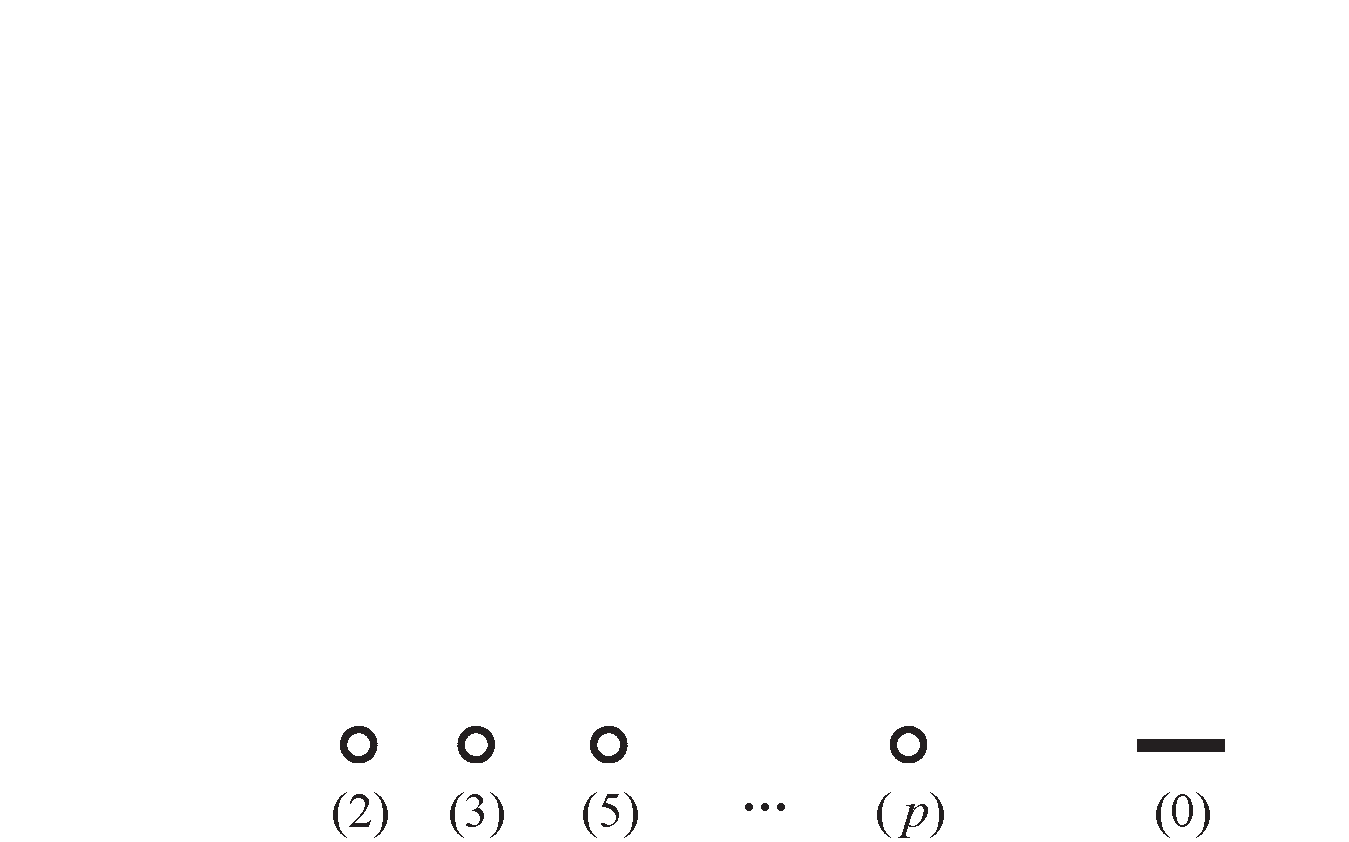
\includegraphics[width=4.25in]{SpecZ.pdf}
  \end{center}
  where the circles are closed points and zero has closure $\Spec\mathbf{Z}$.
  Now take $A = \mathbf{Z}$; then, by Exercise $2.4$ we have that $\Hom_\Sch(X,\Spec\mathbf{Z}) \cong \Hom_\Ring(\mathbf{Z},\Gamma(X,\OO_X))$; however, since $\mathbf{Z}$ is the initial object in $\Ring$ \cite[Prop.~11.3.10]{Art11}, the latter set has one element and so there is a unique morphism $X\to\Spec\mathbf{Z}$, i.e., $\Spec\mathbf{Z}$ is the final object in $\Sch$.
\end{proof}

\begin{problem}
  Describe the spectrum of the zero ring, and show that it is an initial object for the category of schemes. (According to our conventions, all ring homomorphisms must take $1$ to $1$. Since $0=1$ is the zero ring, we see that each ring $R$ admits a unique homomorphism to the zero ring, but that there is no homomorphism from the zero ring to $R$ unless $0 = 1$ in $R$.)
\end{problem}
\begin{proof}
  The spectrum of the zero ring is the empty set with the trivial sheaf $\OO_{\Spec 0}(\emptyset) = 0$. Any scheme $(X,\OO_X)$ thus has a unique morphism defined by the morphism $\emptyset \to X$ on topological spaces and the morphism $\OO_X(U) \to 0$ on sections.
\end{proof}

\begin{problem}
  Let $X$ be a scheme. For any $x \in X$, let $\OO_x$ be the local ring at $x$, and $\mathfrak{m}_x$ its maximal ideal. We define the \emph{residue field} of $x$ on $X$ to be the field $k(x) = \OO_x/\mathfrak{m}_x$. Now let $K$ be any field. Show that to give a morphism of $\Spec K$ to $X$ it is equivalent to give a point $x \in X$ and an inclusion map $k(x) \to K$.
\end{problem}
\begin{proof}
  Suppose a point $x \in X$ and an inclusion map $\iota \colon k(x) \to K$ are
  given. Let $f\colon \Spec K \to X$ be the continuous map such that
  $f(\mathfrak{0}) = x$, where $\mathfrak{0}$ is the unique point
  corresponding to the $0$ ideal in $K$. It remains to give a (local) map of
  sheaves $f^\#\colon \OO_X \to f_*\OO_{\Spec K}$. We note that
  \begin{equation*}
    f_*\OO_{\Spec K}(U) = \OO_{\Spec K}(f^{-1}(U)) = \left\{
    \begin{alignedat}{3}
      \OO_{\Spec K}(\emptyset) &= 0 & \text{if}\ x \notin U\\
      \OO_{\Spec K}(\{\mathfrak{0}\}) &= K & \text{if}\ x \in U
    \end{alignedat}
    \right.
  \end{equation*}
  Thus, $f^\#(U)$ must be the zero map if $x \notin U$, and if $x \in U$, we can
  define it as the composition
  \begin{equation}\label{eq:fhash}
    \begin{tikzcd}[row sep=tiny,column sep=large]
      \OO_X(U)\arrow{dd}[swap]{\rho_{UV}}\arrow{dr}
      \arrow[bend left=15]{drrr}{f^\#(U)}\\
      & \OO_{X,x} \rar{\mathrm{residue}} & k(x) \rar[hook]{\iota} & K\\
      \OO_X(V)\arrow{ur}\arrow[bend right=15]{urrr}[swap]{f^\#(V)}
    \end{tikzcd}
  \end{equation}
  where the map respects restriction $\rho_{UV}$ by the commutativity of the
  diagram above, using the fact that $\OO_{X,x}$ is the direct limit of the
  system on the left.
  \par Now suppose we are given a morphism $(f,f^\#)\colon\Spec K \to X$ of
  schemes; then, since $\Spec K = \{\mathfrak{0}\}$, the corresponding map on
  topological spaces is uniquely determined by the image of $(0)$ in $X$; call this
  $x$. Then, for all open sets $x \in V \subset U$, we get the diagram
  \eqref{eq:fhash} above, where the map $\OO_{X,x} \to K$ factors through $k(x)$
  by the universal property of the quotient since the map $\OO_{X,x} \to K$ is
  local, hence the inverse image of $\mathfrak{0}$ in $\OO_{X,x}$ is
  $\mathfrak{m}_x$ and factors through $k(x)$ uniquely by the universal property
  of the quotient, giving the map $\iota$ above which is an injection since it
  is a ring homomorphism of fields.
  \par Now since the constructions in both directions were induced canonically by
  universal properties, the two directions are mutually inverse, hence giving a
  morphism $\Spec K \to X$ is equivalent to giving a point $x \in X$ and a map
  $k(x) \hookrightarrow K$.
\end{proof}

\begin{problem}
  Let $X$ be a scheme. For any point $x \in X$, we define the \emph{Zariski tangent space} $T_x$ to $X$ at $x$ to be the dual of the $k(x)$-vector space $\mathfrak{m}_x/\mathfrak{m}_x^2$. Now assume that $X$ is a scheme over a field $k$, and let $k[\varepsilon]/\varepsilon^2$ be the \emph{ring of dual numbers} over $k$. Show that to give a $k$-morphism of $\Spec k[\varepsilon]/\varepsilon^2$ to $X$ is equivalent to giving a point $x \in X$, \emph{rational over $k$} (i.e., such that $k(x) = k$), and an element of $T_x$.
\end{problem}
\begin{proof}
  Suppose a rational point $x \in X$ and an element $\eta \in T_x =
  \Hom_k(\mathfrak{m}_x/\mathfrak{m}_x^2,k)$ are given. On topological spaces, we
  define the map $\varphi\colon \Spec k[\varepsilon]/\varepsilon^2 \to X$ to be the
  map sending the unique maximal ideal $(\varepsilon)$ in $\Spec
  k[\varepsilon]/\varepsilon^2$ to $x \in X$. Now $\OO_{X,x}$ as a $k$-vector space
  has a subspace $\mathfrak{m}_x$ such that the quotient by this subspace is
  $\OO_{X,x}/\mathfrak{m}_x = k(x) = k$ by assumption, hence we have an isomorphism
  $\OO_{X,x} \cong k \oplus \mathfrak{m}_x$ of $k$-vector spaces. We can therefore
  define the map
  \begin{equation*}
    \begin{tikzcd}[row sep=0,column sep=small]
      \mathllap{\psi\colon} \OO_{X,x} \rar{\sim} & k \oplus \mathfrak{m}_x \rar &
      \dfrac{k[\varepsilon]}{\varepsilon^2}\\
      & (a,b) \rar[mapsto] & a + \eta(\overline{b})\varepsilon
    \end{tikzcd}
  \end{equation*}
  where $\overline{b}$ denotes reduction mod $\mathfrak{m}_x^2$.
  We claim this defines a $k$-algebra homomorphism. The fact that $\psi$
  respects additivity and multiplication by scalars in $k$ follows by the fact that
  $\psi$ is a map of vector spaces by construction, and so it suffices to show it
  respects multiplication. By the identification above, write two elements of
  $\OO_{X,x}$ as $a_1 + b_1$ and $a_2 + b_2$ where $a_i \in k$ and $b_i \in
  \mathfrak{m}_x$. Then,
  \begin{equation*}
    \psi((a_1 + b_1)(a_2 + b_2) = \psi(a_1a_2 + a_1b_2 + a_2b_1 + a_2b_2) =
    a_1a_2 + a_1\eta(\overline{b_2})\varepsilon + a_2\eta(\overline{b_1})\varepsilon
  \end{equation*}
  since $\eta(\overline{a_2b_2}) = 0$ by the fact that $a_2b_2 \equiv 0 \bmod
  \mathfrak{m}_x^2$. But then
  \begin{equation*}
    \psi(a_1+b_1)\psi(a_2+b_2) = (a_1 + \eta(\overline{b_1})\varepsilon)(a_2 +
    \eta(\overline{b_2})\varepsilon) = a_1a_2 + a_1\eta(\overline{b_2})\varepsilon +
    a_2\eta(\overline{b_1})\varepsilon
  \end{equation*}
  since $\varepsilon^2 = 0$, which are equal; thus, $\psi$ respects
  multiplication as well, and is a $k$-algebra homomorphism.
  \par Now we want to construct $f^\#$. We note that
  \begin{equation*}
    f_*\OO_{\Spec k[\varepsilon]/\varepsilon^2}(U) =
    \OO_{\Spec k[\varepsilon]/\varepsilon^2}(f^{-1}(U)) = \left\{
    \begin{alignedat}{3}
      \OO_{\Spec k[\varepsilon]/\varepsilon^2}(\emptyset) &= 0 & \text{if}\ x \notin U\\
      \OO_{\Spec k[\varepsilon]/\varepsilon^2}(\{\mathfrak{0}\}) &= k[\varepsilon]/\varepsilon^2 & \text{if}\ x \in U
    \end{alignedat}
    \right.
  \end{equation*}
  hence the map $f^\#(U)$ must be the zero map if $x \notin U$, and for $x \in
  U$, we can define $f^\#(U)$ to be the composition
  \begin{equation*}
    \begin{tikzcd}[row sep=tiny]
      \OO_X(U)\arrow{dd}[swap]{\rho_{UV}}\arrow{dr}
      \arrow[bend left=15]{drrr}{f^\#(U)}\\
      & \OO_{X,x} \rar{\sim} & k \oplus \mathfrak{m}_x
      \arrow[hook]{r}[yshift=-1pt]{\psi} & K\\
      \OO_X(V)\arrow{ur}\arrow[bend right=15]{urrr}[swap]{f^\#(V)}
    \end{tikzcd}
  \end{equation*}
  where the map respects restriction $\rho_{UV}$ by the commutativity of the
  diagram above, using the fact that $\OO_{X,x}$ is the direct limit of the
  system on the left. Finally, the map $(f,f^\#)$ is a morphism over $\Spec k$
  since the map $f$ on topological spaces are trivially over $\Spec k$ since
  $\Spec k$ is just a point, and the map $f^\#$ is also over $\OO_{\Spec k}$
  since the maps $f^\#(U)$ constructed above are $k$-algebra homomorphisms.
  \par Now suppose we are given a morphism $(f,f^\#)\colon \Spec
  k[\varepsilon]/\varepsilon^2 \to X$ over $\Spec k$. Let $x =
  f((\varepsilon))$. Since $f$ is a $\Spec k$-morphism, we have the commutative
  diagrams
  \begin{equation*}
    \begin{tikzcd}[column sep=tiny]
      \Spec \frac{k[\varepsilon]}{\varepsilon^2} \arrow{rr}{(f,f^\#)}\arrow{dr} & & X\arrow{dl}\\
      & \Spec k
    \end{tikzcd} \overset{\text{stalks}}{\implies} 
    \begin{tikzcd}[column sep=tiny]
      \frac{k[\varepsilon]}{\varepsilon^2}
      \arrow[leftarrow]{rr}{f^\#_{(\varepsilon)}}\arrow[leftarrow]{dr} & &
      \OO_{X,x}\arrow[leftarrow]{dl}\\
      & k
    \end{tikzcd} \overset{\text{residues}}{\implies} \begin{tikzcd}[column sep=tiny]
      k \arrow[leftarrow]{rr}{f^\#_{(\varepsilon)}}\arrow[leftarrow]{dr} & & k(x)\arrow[leftarrow]{dl}\\
      & k
    \end{tikzcd}
  \end{equation*}
  Since our morphisms on stalks are local, we see that the maps on the right are
  all injections, hence $k(x) = k$ and $x$ is rational over $k$. Now note in the
  middle diagram that $f^\#_{(\varepsilon)}(\mathfrak{m}_x) \subset
  (\varepsilon) \subset k[\varepsilon]/\varepsilon^2$, but $(\varepsilon^2) =
  0$ implies that $f\#_{(\varepsilon)}(\mathfrak{m}_x^2) \subset
  (\varepsilon^2) = 0$. Thus, we get a map $\overline{f^\#_{(\varepsilon)}} \in \Hom(\mathfrak{m}_x/\mathfrak{m}_x^2,k) = T_x$ by the universal property of the quotient, since $(\varepsilon) \cong k$ as vector spaces.
  \par Now we note that the two directions are mutually inverse. If we start
  with a rational point $x \in X$ and an element $\eta \in T_x$, then we get the same
  point $x \in X$ by going through both directions, and also get $\eta$ back
  since $\eta$ acted on the subspace $\mathfrak{m}_x$ of $\OO_{X,x}$, and we
  constructed $\overline{f^\#_{(\varepsilon)}}$ by the restricted action on
  $\mathfrak{m}_x \subset \OO_{X,x}$. In the other direction, given a morphism
  of schemes $(f,f^\#)\colon \Spec k[\varepsilon]/\varepsilon^2 \to X$ and going
  through both directions, we get the same map back since as topological spaces
  the constructions composed together give the same unique image $x \in X$ as
  before, and on sheaves we have the same maps since they are the same map on
  stalks, and then by the sheaf property $(3)$.
\end{proof}

\begin{problem}
  If $X$ is a topological space, and $Z$ is an irreducible closed subset of $X$, a \emph{generic point} for $Z$ is a point $\zeta$ such that $Z = \{\zeta\}^-$. If $X$ is a scheme, show that every (nonempty) irreducible closed subset has a unique generic point.
\end{problem}
\begin{proof}
  Let $o(Z)$ denote the intersection of all non-empty open subsets of $Z$; $o(Z) \ne \emptyset$ since otherwise, there exist two disjoint open subsets $U_1,U_2$ of $Z$, and $Z = U_1^c \cup U_2^c$ contradicts irreducibility. Any point $x \in o(Z)$ is generic since if $x \in o(Z)$ is not, $U = X \setminus \overline{\{x\}} \ne \emptyset$ is open, contradicting the definition of $o(Z)$. Now suppose $y \ne x$ is another generic point of $Z$. Then, since the Zariski topology is $T_0$, there exists $U \ni x$ open such that $U \not\ni y$; then, $A = Z \setminus U$ is a closed proper subset of $Z$ which contains $y$, and so $\overline{\{y\}} \subseteq A \subsetneq Z$, i.e., $y$ cannot be a generic point.
\end{proof}

\begin{problem}
  Describe $\Spec \mathbf{R}[x]$. How does its topological space compare to the set $\mathbf{R}$? To $\mathbf{C}$?
\end{problem}
\begin{proof}[Solution]
  $\mathbf{R}[x]$ is a PID so all irreducibles are prime; thus, $\Spec \mathbf{R}[x]$ consists of prime ideals generated by irreducible polynomials and the generic point $(0)$. These prime ideals are closed, and are of the form $(x-\alpha)$ for $\alpha \in \mathbf{R}$ and $(x-\beta)(x-\overline{\beta})$ for $\beta \in \mathbf{C} \setminus \mathbf{R}$.
  \par We have the following maps of sets:
  \begin{equation*}
    \begin{tikzcd}[row sep=0em]
      \mathbf{R} \rar & \mathbf{C} \rar & \Spec\mathbf{R}[x]\\
      \alpha \arrow[mapsto]{rr} & & (x-\alpha)\\
      & \beta \arrow[mapsto]{r} & (x-\beta)(x-\overline{\beta})
    \end{tikzcd}
  \end{equation*}
  where the map $\mathbf{C} \to \Spec\mathbf{R}[x]$ is defined as for $\mathbf{R}$ when $\beta \in \mathbf{R}$. Then, $\mathbf{R} \hookrightarrow \Spec \mathbf{R}[x]$ is an injection, but the image of $\mathbf{R}$ is neither open nor closed, and does not have a generic point. The map from $\mathbf{C}$ is generically two-to-one on the image, but again, the image is neither open nor closed.
\end{proof}

\begin{problem}
  Let $k = \mathbf{F}_p$ be the finite field with $p$ elements. Describe $\Spec k[x]$. What are the residue fields of its points? How many points are there with a given residue field?
\end{problem}
\begin{proof}[Solution]
  Again, $\Spec k[x]$ consists of prime ideals generated by irreducible polynomials with the generic point $(0)$; note these are also maximal hence closed. The residue field at $(0)$ is the rational function field over $k$. If a maximal ideal is generated by a polynomial of degree $d$, then $k(x) = \mathbf{F}_{p^d}$. Finally, the number of irreducible polynomials of a given degree $d$, hence the number of points with a given residue field, is given by the M\"obius inversion formula \cite[p.~588]{DF04}:
  \begin{equation*}
    \psi(d) = \frac{1}{d} \sum_{\ell \mid d} \mu(\ell)p^{d/\ell},
  \end{equation*}
  where
  \begin{equation*}
    \mu(\ell) = \begin{cases}
      1 & \text{if}~\ell = 1,\\
      0 & \text{if $\ell$ has a square factor},\\
      (-1)^r & \text{if $\ell$ has $r$ distinct prime factors}.
    \end{cases}\qedhere
  \end{equation*}
\end{proof}

\begin{problem}
  \emph{Glueing Lemma}. Generalize the glueing procedure described in the text $(2.3.5)$ as follows. Let $\{X_i\}$ be a family of schemes (possibly infinite). For each $i \ne j$, suppose given an open subset $U_{ij} \subseteq X_i$, and let it have the induced scheme structure $(\mathrm{Ex}.~2.2)$. Suppose also given for each $i \ne j$ an isomorphism of schemes $\varphi_{ij}\colon U_{ij} \to U_{ji}$ such that $(1)$ for each $i,j$, $\varphi_{ji} = \varphi_{ij}^{-1}$, and $(2)$ for each $i,j,k$, $\varphi_{ij}(U_{ij} \cap U_{ik}) = U_{ji} \cap U_{jk}$, and $\varphi_{ij} = \varphi_{jk} \circ \varphi_{ij}$ on $U_{ij} \cap U_{ik}$. Then show that there is a scheme $X$, together with morphisms $\psi_i\colon X_i \to X$ for each $i$, such that $(1)$ $\psi_i$ is an isomorphism of $X_i$ onto an open subscheme of $X$, $(2)$ the $\psi_i(X_i)$ cover $X$, $(3)$ $\psi_i(U_{ij}) = \psi_i(X_i) \cap \psi_j(X_j)$ and $(4)$ $\psi_i = \psi_j \circ \varphi_{ij}$ on $U_{ij}$. We say that $X$ is obtained by \emph{glueing} the schemes $X_i$ along the isomorphisms $\varphi_{ij}$. An interesting special case is when the family $X_i$ is arbitrary, but the $U_{ij}$ and $\varphi_{ij}$ are all empty. Then the scheme $X$ is called the \emph{disjoint union} of the $X_i$, and is denoted $\coprod X_i$.
\end{problem}
\begin{proof}
  Define the topological space on $X$ to be
  \begin{equation*}
    X \coloneqq \frac{\displaystyle\coprod X_i}{\varphi_{ij}(x) \sim x},
  \end{equation*}
  where the equivalence relation runs over all $x \in U_{ij}$ and all $i \ne j$,
  with the quotient topology; hypothesis $(1)$ ensures symmetry of our
  equivalence relation and $(2)$ ensures transitivity. Let $\psi_i\colon X_i \to
  X$ denote the inclusion map $X_i \to \coprod X_i/\sim$; it is a homeomorphism
  by definition of the disjoint union and quotient topologies. The $\psi_i(X_i)$
  then form an open cover of $X$, proving $(2)$. By Exercise I.$1.22$, we can glue
  the $\OO_{X_i}$ together to form a sheaf $\OO_X$ on $X$ using the maps on
  sheaves in hypothesis $(2)$. This makes $X$ a scheme since for any $x \in X$,
  we can choose a neighborhood small enough that it is contained in a $X_i$, and
  $X_i$ is locally affine. The $\psi_i$ form morphisms of locally ringed spaces
  by the map $\psi_i$ defined above on topological spaces, with the maps on
  sheaves obtained by Exercise I.$1.22$, proving $(1)$. $(3)$ follows by
  definition of the quotient space, as does $(4)$ on the level of topological
  spaces, and the corresponding property on sheaves is obtained by the glueing
  operation on sheaves in Exercise I.$1.22$.
\end{proof}


\begin{problem}
  A topological space is \emph{quasi-compact} if every open cover has a finite subcover.
  \begin{enuma}
    \item Show that a topological space is noetherian $(\mathrm{I},\S1)$ if and only if every open subset is quasi-compact.
    \item If $X$ is an affine scheme, show that $\Sp(X)$ is quasi-compact, but not in general noetherian. We say a scheme $X$ is \emph{quasi-compact} if $\Sp(X)$ is.
    \item If $A$ is a noetherian ring, show that $\Sp(\Spec A)$ is a noetherian topological space.
    \item Give an example to show that $\Sp(\Spec A)$ can be noetherian even when $A$ is not.
  \end{enuma}
\end{problem}
\begin{proof}[Proof of $(a)$]
  Suppose our topological space $X$ is noetherian. Let $U \subseteq X$, and let $A_1 \supseteq A_2 \supseteq A_3 \supseteq \cdots$ be a descending chain of closed sets in $Y$; write $A_i = Y \cap V_i$ for $V_i \subseteq X$ closed. Then, $V_1 \supsetneq V_1 \cap V_2 \supsetneq V_1 \cap V_2 \cap V_3 \supsetneq \cdots$ stabilizes since $X$ is noetherian, and so $A_1 \supseteq A_2 \supseteq A_3 \supseteq \cdots$ does as well. Now suppose $Y = \bigcup_{\alpha \in A} Y_\alpha$ is an open covering of $Y$ that has no finite subcover. We construct $\alpha_i$ inductively as follows: if $Y \ne Y_{\alpha_1} \cup \cdots \cup Y_{\alpha_n}$, then choose $\alpha_{n+1}$ such that $Y_{\alpha_{n+1}} \not\subseteq Y_{\alpha_1} \cup \cdots Y_{\alpha_n}$. Then,
  \begin{equation*}
    Y \supsetneq (Y \setminus Y_{\alpha_1}) \supsetneq (Y \setminus (Y_{\alpha_1} \cup Y_{\alpha_2})) \supsetneq \cdots
  \end{equation*}
  is a strictly decreasing chain of closed sets that does not stabilize, contradicting that $Y$ is noetherian.
  \par Now suppose that $X$ is such that every open subset is quasi-compact. Let $U_1 \subseteq U_2 \subseteq \cdots$ be an ascending chain of open subsets of $X$. Then, $\bigcup U_i$ has a finite subcover by assumption, and so the chain must stabilize, i.e., $X$ is noetherian.
\end{proof}
\begin{proof}[Proof of $(b)$]
  Suppose $X = \Spec R$. Recall that the sets $D(f)$ for $f \in R$ form a basis of $X$, and so any open cover of $X$ has a refinement of the form $\bigcup X_{f_\alpha}$. Thus,
  \begin{align*}
    X = \bigcup_{\alpha \in A} X_{f_\alpha} &\iff 1 \in \braket{f_\alpha}_{\alpha \in A}\\
    &\iff 1 = h_1f_1 + \cdots + h_mf_m\\
    &\iff X = D(f_1) \cup \cdots \cup D(f_m),
  \end{align*}
  and $X$ is therefore quasicompact.
  \par Now suppose $X = \Spec k[x_1,x_2,\ldots]$. Then, $V(x_1) \supsetneq V(x_1,x_2) \supsetneq \cdots$ is a descending chain that does not stabilize.
\end{proof}
\begin{proof}[Proof of $(c)$]
  If $V(I_1) \supseteq V(I_2) \supseteq V(I_3) \supseteq \cdots$ is a descending chain, we have the corresponding ascending chain $\sqrt{I_1} \subseteq \sqrt{I_2} \subseteq \sqrt{I_3} \subseteq \cdots$ in $A$, which stabilizes since $A$ is noetherian; thus, the descending chain of closed sets also stabilizes.
\end{proof}
\begin{proof}[Proof of $(d)$]
  Let $A = k[x_1,x_2,\ldots]/(x_1^2,x_2^2,\ldots)$, and $X = \Spec A$. $X$ then consists of one point, $(x_1,x_2,\ldots)$, since this is the only prime ideal in $A$ (it is the only prime ideal that contains $(x_1^2,x_2^2,\ldots)$ in $k[x_1,x_2,\ldots]$), and so is trivially noetherian. The ring, however, is not noetherian since $(x_1) \subsetneq (x_1,x_2) \subsetneq \cdots$ is an ascending chain that does not stabilize.
\end{proof}

\begin{problem}\mbox{}
  \begin{enuma}
    \item Let $S$ be a graded ring. Show that $\Proj S = \emptyset$ if and only if every element of $S_+$ is nilpotent.
    \item Let $\varphi\colon S \to T$ be a graded homomorphism of graded rings (preserving degrees). Let $U = \{\mathfrak{p} \in \Proj T \vert \mathfrak{p} \not\supseteq \varphi(S_+)\}$. Show that $U$ is an open subset of $\Proj T$, and show that $\varphi$ determines a natural morphism $f \colon U \to \Proj S$.
    \item The morphism $f$ can be an isomorphism even when $\varphi$ is not. For example, suppose that $\varphi_d\colon S_d \to T_d$ is an isomorphism for all $d \ge d_0$, where $d_0$ is an integer. Then show that $U = \Proj T$ and the morphism $f \colon \Proj T \to \Proj S$ is an isomorphism.
    \item Let $V$ be a projective variety with homogeneous coordinate ring $S$ $(\mathrm{I},\S2)$. Show that $t(V) \cong \Proj S$.
  \end{enuma}
\end{problem}
\begin{proof}[Proof of $(a)$]
  $S_+ \subseteq \mathfrak{N}(S) \implies S_+ \subseteq \mathfrak{p}$ for all prime ideals $\mathfrak{p}$, and so $\Proj S = \emptyset$.
  \par Conversely, suppose $\Proj S = \emptyset$, and consider $f \in S_+$ homogeneous. Then, $D(f) = \emptyset \implies \Spec S_{(f)} = \emptyset$. Thus, $S_{(f)} = 0$, and so $1/f^n = 0$, and $f^n = 0$ for some $n$, i.e., $f$ is nilpotent. Homogeneous elements generate $S_+$ so $S_+ \subseteq \mathfrak{N}(S)$.
\end{proof}
\begin{proof}[Proof of $(b)$]
  $\varphi(S_+)$ is a homogeneous ideal, and so $U^c = \{\mathfrak{p} \in \Proj T \vert \mathfrak{p} \supseteq \varphi(S_+)\}$ is closed.
  \par Now $\varphi$ determines a natural morphism $f\colon U \to \Proj S$ by $f(x) = \varphi^{-1}(x)$. This is continuous since $f^{-1}(V(I)) = V(\varphi(I))$. We then define the sheaf morphism $f^\#\colon \OO_S(V) \to \OO_T(f^{-1}(V))$ for $V \subseteq \Proj S$ by composing a section $s\colon V \to \coprod S_{\varphi^{-1}(\mathfrak{p})}$ where the $\mathfrak{p}\in V$, with the morphisms $\varphi_{(\mathfrak{p})}\colon S_{\varphi^{-1}(\mathfrak{p})} \to T_{\mathfrak{p}}$.
\end{proof}
\begin{proof}[Proof of $(c)$]
  Let $\mathfrak{p} \in \Proj T$; choose $t \in T_+ \setminus \mathfrak{p}$. $\deg t \ge 1$, and so $\deg t^k \ge d_0$ for some $k$. Since $\varphi_d$ is an isomorphism for all $d \ge d_0$, there exists $s \in S_+$ such that $\varphi(s) = t^k \notin \mathfrak{p}$, and so $\varphi(S_+) \not\subseteq \mathfrak{p}$. Thus, $\mathfrak{p} \in U$, and so $U = \Proj T$.
  \par Now choose $t_i$ that generate $T_+$. Then, $\bigcup D_+(t_i) = \Proj T$ forms an open cover; similarly, $\bigcup D_+(t_i^{d_0}) = \Proj T$. Since we can find $s_i$ such that $\varphi(s_i) = t_i^{d_0}$ by the fact that $\varphi$ is an isomorphism for $d \ge d_0$. We then have a morphism of affine schemes $f_i\colon D(t_i) \to D(s_i)$ induced by the restriction of $f$; to show $f$ is an isomorphism, it then suffices to show that each $f_i$ is an isomorphism, for gluing is immediate since we are just taking restrictions of $f$. We note $\cup D(s_i) = \Proj S$, for if not, and $\mathfrak{p} \ni s_i$ for every $i$, then $f(\mathfrak{p}) \ni t_i$ for all $i$, i.e., $f(\mathfrak{p}) \supseteq T_+$.
  \par Now to see that $f$ is injective, it suffices to show injectivity on each $i$. Suppose $f/s^n \mapsto 0$; then, $0 = t^m\varphi(f) = \varphi(s^m)\varphi(f)$ for some $m$. Thus, $s^mf \in \ker\varphi$. Exponentiating by a power large enough makes $s^mf \in S_d$ which is isomorphic to $T_d$; thus, $s^mf = 0$ and $f/s^m = 0$, and so $f$ is injective. Now if $f/t^n \in T_{(t)}$, this is equal to $t^{d_0}f/t^{n+d_0}$; but then, $t^{d_0}f$ has high enough degree such that it has preimage in $S$; our morphism is therefore surjective as well.
\end{proof}
\begin{proof}[Proof of $(d)$]
  Recall $t(V)$ is the set of all (nonempty) irreducible closed subsets of $V$; these are defined by $I$ homogeneous ideals not equal to $S_+$, and so the map $f$ sending an irreducible closed subset of $V$ defined by an ideal $I$ to $V(I)$ of its associated ideal is a bijection by Exercise I.2.4. Now, recall the closed sets of $t(V)$ are of the form $t(W)$ for $W$ closed in $V$; to check continuity, it suffices to check continuity for basis elements. But the preimage of $D_+(f)$ for any $f$ is still open by definition of $t(V)$, and similarly the image of any (closed) basis element $t(W)$ for $W$ defined by $I$ closed in $V$ is the ideal $\sqrt{I}$, which is still closed.
  \par We claim that we have an isomorphism on sheaves. Recall the sheaf is given by $(t(V),\alpha_*(\OO_V))$. We then want to define $f^\#\colon \OO_{\Proj S}(U) \to f_*\OO_{t(V)}(U) = \OO_{V}(\alpha^{-1}(f^{-1}(U)))$. But this works since local sections on one side uniquely determine local sections on the other.
\end{proof}

\begin{problem}\mbox{}
  \begin{enuma}
    \item Let $V$ be a variety over the algebraically closed field $k$. Show that a point $P \in t(V)$ is a closed point if and only if its residue field is $k$.
    \item If $f\colon X \to Y$ is a morphism of schemes over $k$, and if $P \in X$ is a point with residue field $k$, then $f(P) \in Y$ also has residue field $k$.
    \item Now show that if $V,W$ are any two varieties over $k$, then the natural map
      \begin{equation*}
        \Hom_{\Var}(V,W) \to \Hom_{Sch/k}(t(V),t(W))
      \end{equation*}
      is bijective. (Injectivity is easy. The hard part is to show it is surjective.)
  \end{enuma}
\end{problem}
\begin{proof}[Proof of $(a)$]
  Suppose $P \in t(V)$ with $k(P) = k$. Then $P$ corresponds to a maximal ideal $\mathfrak{m}_i$ in each affine chart $\Spec A_i$ since a subset of $t(V)$ is closed if and only if its restriction is closed in every affine chart; thus it is itself a closed point.
  \par Now suppose $P$ is a closed point; then, it is closed in some open affine chart $\Spec A$. There, $P$ is a maximal ideal, and so $k(P) = \OO_{X,P}/\mathfrak{m}_P = k$.
\end{proof}
\begin{proof}[Proof of $(b)$]
  Since $f$ is a $k$-morphism, we have the commutative diagrams
  \begin{equation*}
    \begin{tikzcd}[column sep=tiny]
      X \arrow{rr}{f}\arrow{dr} & & Y\arrow{dl}\\
      & \Spec k
    \end{tikzcd} \overset{\text{stalks and residue}}{\implies} 
    \begin{tikzcd}[column sep=tiny]
      k \arrow[leftarrow]{rr}{f^\#_{(P)}}\arrow[leftarrow]{dr} & & k(P)\arrow[leftarrow]{dl}\\
      & k
    \end{tikzcd}
  \end{equation*}
  Since our morphisms on stalks are local, we see that the maps on the right are all injections, hence $k(P) = k$.
\end{proof}
\begin{proof}[Proof of $(c)$]
  Define the map by having $\varphi\colon V \to W$ map to the extension of $\overline{\varphi}$ onto all of $t(V)$ by mapping an irreducible closed subset to the closure of its image. Note that $P$ closed maps to $\overline{\varphi}(P)$ closed as well by $(b)$. This implies injectivity, since $\varphi \ne \psi$ implies they act differently on some point $P \in V$, and so their extensions will as well.
  \par Now, for surjectivity, suppose $\psi\colon t(V) \to t(W)$. We claim that $\varphi = \psi\vert_V$ maps to $\psi$; this is clear since continuous maps were defined such that $\psi(P) = \overline{\{P\}}$ in the first place, and by $(b)$ closed points are mapped to closed points. It therefore suffices to show $\psi$ is regular. Let $U \subseteq W$ be an affine chart; it has preimage $\psi^{-1}(U)$; restricting as necessary we can assume we have $V \supset U' \to U \subset W$ a map between affine charts. But recall that regular maps are given uniquely by maps between rings of sections by Prop.~I.3.5; in our case, we have the ring maps given by the ring maps on sections between $\OO_{t(W)}(U) \to \OO_{t(V)}(U')$, and so we are done.
\end{proof}

\begin{problem}
  Let $X$ be a scheme, and let $f \in \Gamma(X,\OO_X)$, and define $X_f$ to be the subset of points $x \in X$ such that the stalk $f_x$ of $f$ at $x$ is not contained in the maximal ideal $\mathfrak{m}_x$ of the local ring $\OO_x$.
  \begin{enuma}
    \item If $U = \Spec B$ is an open \emph{affine} subscheme of $X$, and if $\overline{f} \in B = \Gamma(U,\OO_X\vert_U)$ is the restriction of $f$, show that $U \cap X_f = D(\overline{f})$. Conclude that $X_f$ is an open subset of $X$.
    \item Assume that $X$ is quasi-compact. Let $A = \Gamma(X,\OO_X)$, and let $a \in A$ be an element whose restriction to $X_f$ is $0$. Show that for some $n > 0$, $f^na = 0$.
    \item Now assume that $X$ has a finite cover by open affines $U_i$ such that each intersection $U_i \cap U_j$ is quasi-compact. (This hypothesis is satisfied, for example, if $\Sp(X)$ is noetherian.) Let $b \in \Gamma(X_f,\OO_{X_f})$. Show that for some $n > 0$, $f^nb$ is the restriction of an element of $A$.
    \item With the hypothesis of $(c)$, conclude that $\Gamma(X_f,\OO_f) \cong A_f$.
  \end{enuma}
\end{problem}
\begin{proof}[Proof of $(a)$]
  Suppose $x \in U \cap X_f$; then, since $x = \mathfrak{p}$ for some prime in $B$, $f_x \notin \mathfrak{m}_x \iff \overline{f} \notin \mathfrak{p} \iff x \in D(\overline{f})$, since by the definition of stalk $f_x = \overline{f}_x$. Now since we can cover $X_f$ with open sets, it is open.
\end{proof}
\begin{proof}[Proof of $(b)$]
  Since $X$ is quasi-compact, it has a finite affine covering. Now in each
  affine chart $U_i = \Spec B_i$, $U_i \cap X_f = D(\overline{f})$ by $(a)$.
  Since $a \in A$ restricts to $0$ in $X_f$, its restriction to
  $D(\overline{f})$ is $0$ as well. Noting $\OO_X(D(\overline{f})) =
  \OO_{U_i}(D(\overline{f})) = (B_i)_{\overline{f}}$ by Prop.\ $2.2(b)$. Thus, there exists some $n_i$ such that $\overline{f}{}^{n_i}a = 0$, and so taking the maximum $n$ of these $n_i$ over the (finite) affine cover, we see that $f^na = 0$ when restricting to each $U$. By the sheaf property, $f^na = 0$.
\end{proof}
\begin{proof}[Proof of $(c)$]
  Let $U_i = \Spec B_i$; $b$ then has image
  \begin{equation*}
    \frac{b_i}{f_i^{n_i}} \in \OO_X(U_i \cap X_f) = \OO_{\Spec B_i}(D(f_i)) = (B_i)_{f_i}
  \end{equation*}
  by $(a)$, where $f_i$ is the image of $f$ in $\OO_X(U_i)$. Multiplying $b$ by $f^n$ where $n = \max n_i$ gives that $bf^n \in \OO_X(X_f)$ has image $b_if_i^{n-n_i}/1 \in \OO_{\Spec B_i}(D(f_i))$, which lifts to $b_if_i^{n-n_i} \in \Spec B_i$. We now claim that these $b_if_i^{n-n_i}$ lift to some element in $\OO_X(X) = A$. But this is true since on each intersection $(U_i \cap U_j) \cap X_f$, the restrictions satisfy $b_if_{ij}^{n-n_i} - b_jf_{ji}^{n-n_j} = 0$ and so by $(b)$, $f_{ij}^{m_{ij}}(b_if_{ij}^{n-n_i} - b_jf_{ij}^{n-n_j}) = 0$ for some $m_{ij}$. Taking $m = \max m_{ij}$, gluing these sections $b_if_i^{m+n-n_i}$ together produces the element in $A$ we require.
\end{proof}
\begin{proof}[Proof of $(d)$]
  Define the map $\Gamma(X_f,\OO_f) \to A_f$ by mapping $b \mapsto a/f^n$, where $a$ is the element in $(c)$ that restricts to $bf^n$ on $X_f$. This is well defined since if $bf^m$ lifted to $a' \in A$, then assuming without loss of generality $m > n$, the restriction of $f^{n}(f^{m-n}a'-a)$ is zero, and then applying $(b)$. This map is injective since if $b$ was such that $bf^n$ had lift $a$, and $b'$ was such that $b'f^m$ had lift $a'$, then $a/f^n = a'/f^m \implies b = b'$. This map is surjective since if $a/f^n \in A_f$, then $\overline{a} \in b$ lifts to $a$, and so $\overline{a}/\overline{f}^n \mapsto a/f^n$.
\end{proof}

\begin{problem}
  \emph{A Criterion for Affineness}.
  \begin{enuma}
  \item Let $f\colon X \to Y$ be a morphism of schemes, and suppose that $Y$ can be covered by open subsets $U_i$, such that for each $i$, the induced map $f^{-1}(U_i) \to U_i$ is an isomorphism. Then $f$ is an isomorphism.
  \item A scheme $X$ is affine if and only if there is a finite set of elements $f_1,\ldots,f_r \in A = \Gamma(X,\OO_X)$, such that the open subsets $X_{f_i}$ are affine, and $f_1,\ldots,f_r$ generate the unit ideal in $A$.
  \end{enuma}
\end{problem}
\begin{proof}[Proof of $(a)$]
  We first show $f$ is a homeomorphism on topological spaces. If $W \subseteq Y$, then $f^{-1}(W) = \bigcup f^{-1}(W \cap U_i)$ is open, and if $V \subseteq X$, then $f(V) = \bigcup f(V \cap f^{-1}(U_1))$ is open, and so it remains to show $f$ is bijective. $f$ is surjective since very $y \in Y$ is in particular in some $U_i$, and so it has a preimage in $f^{-1}(U_i) \subseteq X$; likewise, $f$ is injective since if $f(x) = f(y) \in U_i$ for some $i$, then they must have the same preimage in $f^{-1}(U_i)$.
  \par Now it remains to show that we have an isomorphism of sheaves. But this is true since we have an isomorphism on stalks by Prop.~1.1.
\end{proof}
\begin{proof}[Proof of $(b)$]
  If $X$ is affine, then we can take $f_1 = 1$ and be done. In the other
  direction, we have a morphism of commutative rings $A \to \Gamma(X,\OO_X)$,
  and so we automatically have a morphism of schemes $\varphi\colon X \to \Spec
  A$ by Exercise 2.4; we want to show this is an isomorphism.
  %We first have the morphisms of commutative rings
  %\begin{equation*}
  %  \begin{tikzcd}
  %    A \rar{\id} \dar & \Gamma(X,\OO_X) \dar \rar[equals] & A \dar\\
  %    A_{f_i} & \Gamma(X_{f_i},\OO_{X_{f_i}}) \rar[equals] & A_{f_i}
  %  \end{tikzcd}
  %\end{equation*}
  %where the vertical maps are the localization. Applying Exercise $2.4$ gives the morphisms of schemes
  %\begin{equation*}
  %  \begin{tikzcd}
  %    X \rar & \Spec A\\
  %    X_{f_i} \uar[hookrightarrow] & D(f_i) \uar[hookrightarrow]
  %  \end{tikzcd}
  %\end{equation*}
  Since $\braket{f_1,\ldots,f_r} = A$, $\Spec A = D(f_1) \cup \cdots \cup
  D(f_r)$ is an open cover. The preimage of each $D(f_i)$ is $X_{f_i}$ by
  construction of the map $X \to \Spec A$ in Exercise 2.4. To show our
  claim, it suffices to show that $\varphi_i \coloneqq
  \varphi\vert_{X_{f_i}}\colon X_{f_i} \to D(f_i)$ is an isomorphism; it
  suffices to show we have an isomorphism $A_{f_i} \to \Gamma(X_{f_i},\OO_X)$ of
  rings since both $X_{f_i}$ and $D(f_i) = \Spec A_{f_i}$ are affine. For
  injectivity, suppose $a/f_i^n \mapsto 0$; then, it vanishes in each $X_i \cap
  X_j = \Spec(A_{f_j})_{f_i}$, so for each $j$ there is some $n_j$ such that
  $a/f_j^{n_j} = 0$ in $A_{f_j}$. Letting $m = \max n_j$ means that $f_i^ma = 0$
  and so $a/f_i^n = 0$ in $A_{f_i}$. For surjectivity, let $a \in A_{f_i} =
  \Gamma(X_{f_i},\OO_X)$ by Exercise 2.16$(d)$. Then,
  $a\vert_{X_{f_i,f_j}} = b_j/f_j^{n_j}$ for some $b_j \in A_{f_j}$ and $n_j$ an
  integer. So, for some $n$ large enough, we have an element $b_j \in A_{f_j}$ such that its restriction on each $X_{f_if_j}$ is $f_i^{n}a$. On triple intersections $X_{f_if_jf_k}$ we have $b_j - b_k = f_i^na - f_i^na = 0$ and so there exists $m_{jk}$ such that $f_i^{m_{jk}}(b_j-b_k) = 0$. Replacing them all with large enough $m$, we have $f_i^mb_j$ for each $X_{f_j}$, and together with $f_i^{n+m}a$ on $X_{f_i}$ we have sections that all agree on intersections. By the sheaf property, we then have a global section $s$ which restricts to $f_i^{n+m}a$ on $X_{f_i}$, and so $s/f_i^{n+m} \mapsto a$ by $\varphi\vert_{X_{f_i}}$.
  \par Finally, by $(a)$ of this problem we are done.
\end{proof}

\begin{problem}
  In this exercise, we compare some properties of a ring homomorphism to the induced morphism of the spectra of the rings.
  \begin{enuma}
    \item Let $A$ be a ring, $X = \Spec A$, and $f \in A$. Show that $f$ is nilpotent if and only if $D(f)$ is empty.
    \item Let $\varphi\colon A \to B$ be a homomorphism of rings, and let $f\colon Y = \Spec B \to X = \Spec A$ be the induced morphism of affine schemes. Show that $\varphi$ is injective if and only if the map of sheaves $f^\#\colon \OO_X \to f_*\OO_Y$ is injective. Show furthermore in that case $f$ is \emph{dominant,} i.e., $f(Y)$ is dense in $X$.
    \item With the same notation, show that if $\varphi$ is surjective, then $f$ is a homeomorphism of $Y$ onto a closed subset of $X$, and $f^\#\colon \OO_X \to f_*\OO_Y$ is surjective.
    \item Prove the converse to $(c)$, namely, if $f\colon Y \to X$ is a homeomorphism onto a closed subset, and $f^\#\colon\OO_X \to f_*\OO_Y$ is surjective, then $\varphi$ is surjective.
  \end{enuma}
\end{problem}
\begin{proof}[Proof of $(a)$]
  $f \in \mathfrak{N}(A) = \bigcap \mathfrak{p}$, where $\mathfrak{p}$ ranges over all prime ideals of $A$ $\iff f \in \mathfrak{p}$ for all $\mathfrak{p} \in \Spec A \iff D(f) = \emptyset$.
\end{proof}
\begin{proof}[Proof of $(b)$]
  If $f^\#$ is injective, then it is injective for $f^\#(X) = \varphi$. Conversely, suppose $\varphi$ is injective. It suffices to show that the map $f_\mathfrak{p}\colon \OO_{\Spec A,\mathfrak{p}} \to f_*\OO_{\Spec B,\mathfrak{p}}$ is injective. We note that, letting $S = \varphi(A \setminus \mathfrak{p})$,
  \begin{align*}
    f_*\OO_{\Spec B,\mathfrak{p}} &= \varinjlim_{U \ni \mathfrak{p}} \OO_{\Spec B}(f^{-1}(U))\\
    &= \varinjlim_{D(a) \ni \mathfrak{p}} \OO_{\Spec B}(f^{-1}(D(a)))\\
    &= \varinjlim_{D(\varphi(a)) \ni \varphi(\mathfrak{p})} \OO_{\Spec B}(D(\varphi(a)))\\
    &= S^{-1}B
  \end{align*}
  where the second line follows since $D(a)$ for $a \in A$ form a basis, and the third line follows since $D(a) \ni \mathfrak{p} \iff a \notin \mathfrak{p} \implies \varphi(a) \notin \varphi(\mathfrak{p})$; the last line is just by definition of the direct limit, since $S = \varphi(A \setminus \mathfrak{p}) = \{\varphi(a) \vert \varphi(\mathfrak{p}) \in D(\varphi(a)) \}$. We note that by \cite[Prop.~3.5]{AM69}, we have that $S^{-1}B \cong B \otimes_A A_\mathfrak{p}$. Injectivity of the map $A \to B$ then ensures $A_\mathfrak{p} \to S^{-1}B \cong B \otimes_A A_\mathfrak{p}$ is also injective by the exactness of direct limits \cite[Ex.~2.19]{AM69}.
  \par To show it is dominant, we consider $W \coloneqq X \setminus \overline{f(Y)}$; suppose $W \ne \emptyset$. $W$ is then covered by basis elements of the form $D(f)$, where $f \in \varphi^{-1}\mathfrak{p}$ for all $\mathfrak{p} \in \Spec B$. But then, $\varphi(f) \in \mathfrak{p}$ for all $\mathfrak{p} \in \Spec B$, and so $\varphi(f)$ is nilpotent; thus, $f$ is also nilpotent by injectivity of $\varphi$ and we have $D(f) = \emptyset$ by $(a)$.
\end{proof}
\begin{proof}[Proof of $(c)$]
  Now suppose $\varphi$ is surjective; this induces an isomorphism $A/\ker\varphi \cong B$, and so we immediately have a bijection between primes containing $\ker\varphi$ in $A$ and primes in $B$. We claim this is a homeomorphism $\Spec B \to V(\ker\varphi) \subset \Spec A$; since the induced map on topological spaces is automatically continuous, it suffices to show it is closed. But this is true since a basis element $D(f) \subset \Spec B$ maps to $D(\varphi^{-1}(f))$ in $\Spec A$, whose intersection with $V(\ker\varphi)$ is also open by definition of the induced topology on $V(\ker\varphi)$. The map $f^\#$ is clearly surjective since it induces the map $A_\mathfrak{p} \to B \otimes_A A_\mathfrak{p}$ on stalks, which is surjective by the right exactness of the tensor product.
\end{proof}
\begin{proof}[Proof of $(d)$]
  Since $f^\#$ is surjective, it is surjective on every stalk, i.e., the maps $A_{\mathfrak{p}} \to B \otimes_A A_\mathfrak{p}$ are surjective for all $\mathfrak{p}$. But $A \to B$ is surjective if and only if $A_{\mathfrak{p}} \to B \otimes_A A_\mathfrak{p}$ is surjective for all prime $\mathfrak{p}$ by \cite[Prop.~3.9]{AM69}.
\end{proof}

\begin{problem}
  Let $A$ be a ring. Show that the following conditions are equivalent:
  \begin{enumi}
    \item $\Spec A$ is disconnected;
    \item there exist nonzero elements $e_1,e_2 \in A$ such that $e_1e_2 = 0$, $e_1^2 = e_1$, $e_2^2 = e_2$, $e_1 + e_2 = 1$ (these elements are called \emph{orthogonal idempotents});
    \item $A$ is isomorphic to a direct product $A_1 \times A_2$ of two nonzero rings.
  \end{enumi}
\end{problem}
\begin{proof}
  $(i) \Rightarrow (ii)$. Say $\Spec A = U_1 \amalg U_2$. These are also closed, so $U_1 = V(I_1)$, $U_2 = V(I_2)$. Then, $V(0) = X = U_1 \amalg U_2 = V(I_1\cdots I_2)$, and so $I_1I_2 \subset \sqrt{0}$. Likewise, $V(A) = \emptyset = U_1 \cap U_2 = V(I_1 + I_2)$, and so $\sqrt{I_1 + I_2} = R$. By \cite[Ex.~1.13iv]{AM69}, this implies $I_1 + I_2 = R$. Thus, $x_1 + x_2 = 1$ for some $x_1 \in I_1$, $x_2 \in I_2$.
  \par Now since $I_1I_2 \subset \sqrt{0}$, we have $(x_1x_2)^m = 0$ for some $m$. Then, we have
  \begin{equation*}
    1 = (x_1 + x_2)^{2m} = \underbrace{x_1^{2m} + \cdots + \binom{2m}{m+1} x_1^{m+1}x_2^{m-1}}_{e_1} + \underbrace{\binom{2m}{m}x_1^mx_2^m + \cdots + x_2^{2m}}_{e_2}
  \end{equation*}
  Then, we have $e_1e_2 = 0$, $e_1^2 = e_1$, and $e_2^2 = e_2$.
  \par $(ii) \Rightarrow (iii)$. We first see that $A = \braket{e_1} \oplus \braket{e_2} = A_1 \times A_2$ where $A_1 = \braket{e_1}$, $A_2 = \braket{e_2}$, for $e_1 + e_2 = 1$, and this is a direct product by the orthogonality relations.
  \par $(iii) \Rightarrow (i)$. If $A \cong A_1 \times A_2$, then letting $e_1$ be the generator of $A_1$ and $e_2$ the generator of $A_2$, we have $A_1 \cong A/\Ann_A e_1$ and $A_2 \cong A/\Ann_A e_2$; thus, we have the partition $\Spec A = V(\Ann_A e_1) \amalg V(\Ann_A e_2)$.
\end{proof}

\subsection{First Properties of Schemes}
\begin{problem}
  Show that a morphism $f \colon X \to Y$ is locally of finite type if and only if for \emph{every} open affine subset $V = \Spec B$ of $Y$, $f^{-1}(V)$ can be covered by open affine subsets $U_j = \Spec A_j$, where each $A_j$ is a finitely generated $B$-algebra.
\end{problem}
\begin{proof}
  $\Leftarrow$ Trivial. $\Rightarrow$ Suppose that $f$ is locally of finite
  type, where $\Spec B_i$ is our cover of $Y$ such that the preimage of each
  $\Spec B_i$ is covered by $\Spec A_{ij}$, where each $A_{ij}$ is a finitely
  generated $B_i$-algebra. $V = \Spec B$ is then covered by $V
  \cap \Spec B_i$'s, and so is covered by distinguished opens $\Spec B_{f_k} =
  \Spec (B_i)_{g_k}$ by Lemma \ref{niketrick}. Now, the preimage of the open
  subsets $\Spec (B_i)_{g_k}$ is covered by $\Spec (A_{ij})_{g_k}$, where we
  consider $g_k$ as an element of $A_{ij}$ via the structure morphism $B_i \to
  A_{ij}$ by \cite[1.21$i$]{AM69}. The $(A_{ij})_{g_k}$ are finitely generated $(B_i)_{g_k}$-algebras, and so we are done since the $B_{f_k} \cong (B_i)_{g_k}$ are finitely generated $B$-algebras.
\end{proof}

\begin{problem}
  A morphism $f\colon X \to Y$ of schemes is \emph{quasi-compact} if there is a cover of $Y$ by open affines $V_i$ such that $f^{-1}(V_i)$ is quasi-compact for each $i$. Show that $f$ is quasi-compact if and only if for \emph{every} open affine subset $V \subseteq Y$, $f^{-1}(V)$ is quasi-compact.
\end{problem}
\begin{proof}
  $\Leftarrow$ Trivial. $\Rightarrow$ Suppose that $f$ is quasi-compact. $V$ is covered by $V \cap V_i$, and so has an open cover by open subsets $D(f_k) \subset V_i$. Since $V$ is affine it is quasi-compact by Exercise $2.13(b)$, and so we can assume this cover is finite. We can cover each $f^{-1}(V_i)$ with open affines $\Spec A_{ij}$; the preimage of the $D(f_k)$ in each $\Spec A_{ij}$ is $\Spec (A_{ij})_{f_k}$, so now we have a finite cover of $f^{-1}(V)$ by open affines $\Spec (A_{ij})_{f_k}$. $f^{-1}(V)$ is therefore quasi-compact, since if we had a cover of $f^{-1}(V)$, it would restrict to finite subcovers of each $\Spec (A_{ij})_{f_k}$, and so lift to a finite subcover of $f^{-1}(V)$ since there are only finitely many $\Spec (A_{ij})_{f_k}$.
\end{proof}

\begin{problem}\mbox{}
  \begin{enuma}
    \item Show that a morphism $f\colon X \to Y$ is of finite type if and only if it is locally of finite type and quasi-compact.
    \item Conclude from this that $f$ is of finite type if and only if for \emph{every} open affine subset $V = \Spec B$ of $Y$, $f^{-1}(V)$ can be covered by a finite number of open affines $U_j = \Spec A_j$, where each $A_j$ is a finitely generated $B$-algebra.
    \item Show also if $f$ is of finite type, then for \emph{every} open affine subset $V = \Spec B \subseteq Y$, and for \emph{every} open affine subset $U = \Spec A \subseteq f^{-1}(V)$, $A$ is a finitely generated $B$-algebra.
  \end{enuma}
\end{problem}
\begin{proof}[Proof of $(a)$]
  $\Leftarrow$ Follows by definition of locally of finite type and Exercise $3.2$. $\Rightarrow$ It suffices to show $f$ is quasi-compact. But if $\Spec A_{ij}$ is our finite cover of $f^{-1}(V_i)$, then $f^{-1}(V_i)$ is the finite union of quasi-compact spaces hence quasi-compact as in Exercise $3.2$.
\end{proof}
\begin{proof}[Proof of $(b)$]
  By $(a)$, $f$ is of finite type if and only if it is locally of finite type and quasi-compact. The claim then follows since the stated condition is exactly the combination of the two conditions in Exercises $3.1$ and $3.2$.
\end{proof}
\begin{proof}[Proof of $(c)$]
  Let $U_j = \Spec A_j$ be the cover of $f^{-1}(V)$ from $(b)$. Let $U = \Spec A \subseteq f^{-1}(V)$. Then, it has a finite cover $U \cap U_j$, and each $U \cap U_j$ can be covered by distinguished opens of $U_j$ that are also distinguished opens of $U$ by Lemma \ref{niketrick}; let these be $U_k = \Spec A_{f_k} = \Spec (A_j)_{g_k}$, and we note that $A_{f_k}$ are finitely generated $B$-algebras by $(b)$. Since $\Spec A$ is affine hence quasi-compact by Exercise $2.13(b)$, we can pick a finite subcover of $U_k$'s.
  \par It remains to show $A$ is a finitely generated $B$-algebra. Let $a \in A$, and choose $f_{k1},\ldots,f_{km} \in A$ that generate $A_{f_k}$ over $B$. There then exists $n$ such that $f_k^na = \sum_\ell g_{k\ell}f_{k\ell}$ for all $k$. Now $(f_k^n)_k = A$ by \cite[Ex.~1.13iv]{AM69}, and so we can represent $a$ as a linear combination of $f_{k\ell}$'s, i.e., $A$ is a finitely generated $B$-algebra.
\end{proof}

\begin{problem}
  Show that a morphism $f\colon X \to Y$ is finite if and only if for \emph{every} open affine subset $V = \Spec B$ of $Y$, $f^{-1}(V)$ is affine, equal to $\Spec A$, where $A$ is a finite $B$-module.
\end{problem}
\begin{proof}
  $\Leftarrow$ Trivial. $\Rightarrow$ Suppose that $f$ is finite. Then, $V$ is
  covered by $V \cap \Spec B_i$, and so is covered by distinguished opens $\Spec
  B_{f_k} = \Spec (B_i)_{g_k}$ by the Lemma \ref{niketrick}; by
  affineness of $V$, we can assume these are finite. Then, the $f_k$ generate
  the unit ideal in $B$. Now, the $f^\#(f_k) \in \Gamma(f^{-1}(V),\OO_X) = A$
  generate the unit ideal in $A$ by the properties of a ring morphism. Moreover,
  since the preimage of the $\Spec B_{f_k}$ is exactly $\Spec A_{f^\#(f_k)}$, we
  see that $f^{-1}(V)$ is affine by Exercise $2.17(b)$, and that by assumption,
  we see that $A_{f^\#(f_k)}$ is a finitely generated $B_{f_k}$-module.
  \par It remains to show that $A$ is a finite $B$-module. Suppose
  $a_{k1},\ldots,a_{km}$ are generators of $A_{f^\#(f_k)}$ over $B_{f_k}$; after
  clearing denominators, we can assume that the generators are in $A$. Then, any
  element $a \in A$ satisfies $f_k^na = \sum_\ell b_\ell a_{k\ell}$ for some
  $b_\ell \in B$, for every $k$, after clearing denominators. By
  \cite[Exc.\ 1.13iv]{AM69}, we then know that any $a$ can be represented as a
  $B$-linear combination of the $a_k\ell$'s, and so the $a_k\ell$'s generate $A$
  over $B$.
\end{proof}


\begin{problem}
  A morphism $f\colon X \to Y$ is \emph{quasi-finite} if for every point $y \in Y$, $f^{-1}(y)$ is a finite set.
  \begin{enuma}
    \item Show that a finite morphism is quasi-finite.
    \item Show that a finite morphism is \emph{closed,} i.e., the image of any closed subset is closed.
    \item Show by example that a surjective, finite-type, quasi-finite morphism need not be finite.
  \end{enuma}
\end{problem}
\begin{proof}[Proof of $(a)$]
  $y \in V$ for some affine open subset $V = \Spec B$. Since $f$ is finite,
  $f^{-1}(V) = \Spec A$ for some $A$ a finite $B$-module. Now, it suffices to
  show that $f^{-1}(y) \cong \Spec A \times_{\Spec B} \Spec k(y)$ is finite by
  Exercise $3.10$. But $\Spec A \times_{\Spec B} \Spec k(y) \cong \Spec(A
  \otimes_B k(y))$ by Thm.~3.3. Since $A$ is a finite $B$-module, we see that $A
  \otimes_B k(y)$ is a finite $k(y)$-module. Thus, $A \otimes_B k(y)$ is a
  finite dimensional $k(y)$-algebra. Now since ideals in $A \otimes_B k(y)$ are
  $k(y)$-vector subspaces, they satisfy the descending chain condition, and so
  $A \otimes_B k(y)$ is artinian. $\Spec A \otimes_B k(y)$ is then discrete by
  \cite[Prop.\ 8.1]{AM69}, and is finite by \cite[Prop.\ 8.3]{AM69}.
\end{proof}
\begin{proof}[Proof of $(b)$]
  Since a closed subset is closed if and only if it is closed in every element
  of an open cover, we can reduce to the case when $X = \Spec A$ and $Y = \Spec
  B$, where $A$ is a finitely generated $B$-module by the fact that $f$ is
  finite. Moreover, since by Exercise 3.11$(b)$ every closed subset of $X$ will
  then be of the form $\Spec A/\mathfrak{a}$, it suffices to show $f(X)$ is closed.
  By \cite[Exc.\ 5.1]{AM69}, it suffices to show $B \to A$ is integral. But this
  is true by \cite[Prop.\ 5.1]{AM69} since $f$ is finite.
\end{proof}
\begin{proof}[Proof of $(c)$]
  Consider the map
  \begin{equation*}
    \Spec k[x]_x \oplus k[x]_{(x-1)} \to \Spec k[x]
  \end{equation*}
  given by the ring homomorphism $\varphi$ such that $1 \mapsto (1,1)$ and $x \mapsto (x,x)$. Now, for any prime ideal $\mathfrak{p} = (f) \subset k[x]$, we see that $\varphi(\mathfrak{p}) = (f,f)$, which is a prime ideal since it is a prime ideal of at least one of $k[x]_x$ or $k[x]_{x-1}$; thus, $\varphi^*$ is surjective. It is of finite type since adjoining $x^{-1},(x-1)^{-1}$ to two copies of $k[x]$ clearly makes $k[x]_x \oplus k[x]_{x-1}$ a finitely generated $k[x]$-algebra. Finally, it is a quasi-finite morphism since $f^{-1}(\mathfrak{p}) = \Spec k[x]_x \oplus k[x]_{(x-1)} \otimes_{k[x]} k(\mathfrak{p}) = \Spec (k[x]_x \otimes k(\mathfrak{p})) \oplus (k[x]_{x-1} \otimes k(\mathfrak{p})) = \Spec k(\mathfrak{p}) \oplus k(\mathfrak{p})$, which is clearly finite. On the other hand, this is not a finite map since $k[x]_x,k[x]_{(x-1)}$ are both not finite $k[x]$-modules, hence $k[x]_x \oplus k[x]_{(x-1)}$ is not a finite $k[x]$-module.
\end{proof}

\begin{problem}
  Let $X$ be an integral scheme. Show that the local ring $\OO_\xi$ of the generic point $\xi$ of $X$ is a field. It is called the \emph{function field} of $X$, and is denoted by $K(X)$. Show also that if $U = \Spec A$ is any open affine subset of $X$, then $K(X)$ is isomorphic to the quotient field of $A$.
\end{problem}
\begin{proof}
  We have that
  \begin{equation*}
    \OO_\xi = \varinjlim_{U \ni \xi} \OO_X(U) = \varinjlim_{U \ni \xi} \OO_{\Spec A}(U) = k(A).
  \end{equation*}
  where $\Spec A$ is an affine neighborhood of $\xi$. Note we know that the image of $\xi$ in $\Spec A$ is the generic point of $\Spec A$ since generic points are unique (Exercise 2.9), and $\overline{\{\xi\}} = \Spec A$ since $\Spec A$ has the subspace topology. This is true for any affine neighborhood, since every affine neighborhood contains the generic point.
\end{proof}

\begin{problem}
  A morphism $f \colon X \to Y$, with $Y$ irreducible, is \emph{generically finite} if $f^{-1}(\eta)$ is a finite set, where $\eta$ is the generic point of $Y$. A morphism $f\colon X \to Y$ is \emph{dominant} if $f(X)$ is dense in $Y$. Now let $f\colon X \to Y$ be a dominant, generically finite morphism of finite type of integral schemes. Show that there is an open dense subset $U \subseteq Y$ such that the induced morphism $f^{-1}(U) \to U$ is finite.
\end{problem}
\begin{proof}
  We first claim that there exists a finite field extension $K(Y) \hookrightarrow K(X)$. Let $Y \supset V = \Spec B \ni \eta$ be an affine neighborhood of the generic point, and let $X \supset f^{-1}(V) \supset U = \Spec A$ be an affine neighborhood contained in the preimage, where $A$ is a finitely generated $B$-algebra by Exercise $3.3(c)$. Then, since $X$ is integral, $A$ is an integral domain.
  \par So, $A$ is finitely generated over $B$ and thus, so is $k(B) \otimes_B A \cong S^{-1}A$ over $k(B)$, where $S = B \setminus 0$. Then, by the Noether normalization lemma \cite[14.G]{Mat70}, we have
  \begin{equation*}
    k(B) \subset k(B)[y_1,\ldots,y_n] \subset S^{-1}A
  \end{equation*}
  where the second extension is integral. This implies that we have a surjection
  \begin{equation*}
    \Spec S^{-1}A \twoheadrightarrow \Spec k(B)[y_1,\ldots,y_n]
  \end{equation*}
  by \cite[Exc.\ 5.10]{AM69}. But $\Spec S^{-1}(A) = \Spec k(B) \otimes_B A = \Spec k(B) \times_{\Spec B} \Spec A$, which is homeomorphic to $f^{-1}(\eta) \cap U$ by Exercise 3.10, and so it is finite since $f$ is generically finite. But $\Spec k(B)[y_1,\ldots,y_n]$ is infinite unless $n = 0$, and so we see $k(B) \subset S^{-1}A$ is an integral extension. But then, since an integral extension of a field is a field by Zariski's lemma \cite[Prop.~4.9]{Rei95}, we see that $S^{-1}A = k(A)$, and is a finite algebraic field extension of $k(A)$. This produces a finite field extension for $K(Y) \hookrightarrow K(X)$ by Exercise $3.6$.
  \par Now choose a set of generators for $A$ over $B$; these then satisfy polynomial equations with coefficients in $k(B)$, and so by clearing denominators they satisfy polynomial equations in $B$. Letting $S$ be the multiplicative set generated by all the leading terms of these polynomials, we have that $S^{-1}A$ is integral over $S^{-1}B$, and so $\Spec S^{-1}A \to \Spec S^{-1}B$ is surjective, and moreover finite.
  \par Now for arbitrary $Y$, any affine neighborhood is dense since $Y$ is irreducible. The proposition now follows by taking $U = \Spec S^{-1}B$ with preimage $\Spec S^{-1}A$ as in the previous paragraph.
\end{proof}

\begin{problem}
  \emph{Normalization}. A scheme is \emph{normal} if all of its local rings are integrally closed domains. Let $X$ be an integral scheme. For each open affine subset $U = \Spec A$ of $X$, let $\tilde{A}$ be the integral closure of $A$ in its quotient field, and let $\tilde{U} = \Spec \tilde{A}$. Show that one can glue the schemes $\tilde{U}$ to obtain a normal integral scheme $\tilde{X}$, called the \emph{normalization} of $X$. Show also that there is a morphism $\tilde{X} \to X$, having the following universal property: for every normal integral scheme $Z$, and for every dominant morphism $f\colon Z \to X$, $f$ factors uniquely through $\tilde{X}$. If $X$ is of finite type over a field $k$, then the morphism $\tilde{X} \to X$ is a finite morphism. This generalizes \emph{(I, Ex.~3.17)}.
\end{problem}
\begin{proof}
  We first claim the universal property holds for $X$ affine. If $X = \Spec A$ is affine, then define $\tilde{X} = \Spec \tilde{A}$; let our morphism $\nu\colon\Spec \tilde{A} \to \Spec A$ be the one induced by the ring morphism $A \hookrightarrow \tilde{A}$. Now we want to show the universal property
  \begin{equation*}
    \begin{tikzcd}[column sep=tiny]
      Z \arrow[dashed]{rr}{\varphi}\arrow{dr}[swap]{f} & & \makebox[\widthof{$\tilde{X}$}][l]{$\Spec \tilde{A}$}\arrow{dl}{\nu}\\
      & \makebox[\widthof{$X$}][c]{$\Spec A$}
    \end{tikzcd}
  \end{equation*}
  where $f$ is dominant. By Exercise II.$2.4$, this
  corresponds to the commutative
  diagram
  \begin{equation*}
    \begin{tikzcd}[column sep=tiny]
      \makebox[\widthof{$Z$}][r]{$\Gamma(Z,\OO_Z)$} & & \arrow[dashed]{ll}[swap]{\varphi^*} \tilde{A}\\
      & A \arrow{ul}{f^*} \arrow[hookrightarrow]{ur}[swap]{\nu^*}
    \end{tikzcd}
  \end{equation*}
  in $\Ring$. Since any element of $\tilde{A}$ is in the fraction field, it is
  of the form $a/b$; we claim that defining the map $\varphi^*$ by having $a/b
  \mapsto f^*(a)/f^*(b)$ works. We first show that $f^*(a)/f^*(b) \in
  \Gamma(Z,\OO_Z)$; this follows since if $g(x)$ is the polynomial $a/b$
  satisfies in $A[x]$, then applying $f^*$ to $g(x)$ on each coefficient gives a
  polynomial satisfied by $f^*(a)/f^*(b)$ by the fact that $f^*$ is a ring
  morphism. Then, $f^*(a)/f^*(b) \in \Gamma(Z,\OO_Z)$ by Lemma \ref{lem:normgs}
  since $\Gamma(Z,\OO_Z)$ is integrally closed.
  \par To show the map $\varphi^*$ is unique, we first show $f^*$ is injective.
  But $f$ is dominant by \cite[Exc.\ $1.21v$]{AM69}, hence $\Ker f^* \subset
  \mathfrak{N}(A) = 0$ since $A$ is an integral domain.
  \par Now we can show $\varphi^*$ is unique. If any other map $\psi^*$
  satisfied the commutative diagram, $\varphi^*(a/1) = f^*(a) = \psi^*(a/1)$,
  and so
  \begin{align*}
    f^*(b)\varphi^*(a/b) &= \varphi^*(b/1)\varphi^*(a/b)\\
    &= \varphi^*(a/1) = f^*(a) = \psi^*(a/1)\\
    &= \psi^*(b/1)\psi^*(a/b) = f^*(b)\psi^*(a/b)
  \end{align*}
  implies $\varphi^*(a/b) = \psi^*(a/b)$ for all $a/b \in \tilde{A}$ by the fact
  that $\tilde{A}$ is a domain, i.e., $\varphi^*$ is unique. By the bijection in
  Exercise II.$2.4$, we then see that $\varphi$ exists and is unique as well. Note that this implies that $\tilde{X}$ is unique up to unique isomorphism just by having $\tilde{X}'$ another normalization, and then switching the roles of $\tilde{X}$ and $\tilde{X}'$.
  \par We would like to show now that if $\nu\colon \tilde{X} \to X$ exists for
  $X = \Spec A$ and $U \subset X$ is an open affine, then $\nu^{-1}(U) \cong
  \tilde{U}$. If $Z \to U$ is a dominant map from a normal integral scheme $Z$,
  then $Z$ becomes a dominant map on $X$ since $X$ is irreducible by Prop.~3.1
  hence any open subset of $U$ is open in $X$ and hence dense in $X$. Thus, the
  map factors uniquely through $\tilde{X}$ by the universal property for
  (affine) normalization proved above, and moreover the image of $\tilde{X}$ is
  in $\nu^{-1}(U)$, so $\nu^{-1}(U)$ satisfies the universal property hence is
  isomorphic to $\tilde{U}$.
  \par Finally, we would like to extend this to the case when $X$ is an
  arbitrary scheme. Suppose $\{X_i\}$ is an open affine cover of $X$; then, for
  each $X_i$, $\nu_i\colon\tilde{X}_i \to X_i$ exists. Now given $i \ne j$, let
  $U_{ij} \subset \tilde{X}_i$ be $\nu_i^{-1}(X_{ij})$, where $X_{ij} = X_i \cap
  X_j$. Then, $U_{ij} \cong \tilde{X}_{ij}$ by the above paragraph, hence by the
  uniqueness of (affine) normalization above, we see that there exist
  isomorphisms $\varphi_{ij}\colon U_{ij} \to U_{ji}$ for all $i \ne j$ that are
  compatible in the sense of Exercise II.$2.12$, since uniqueness up to unique
  isomorphism ensures that $\varphi_{jk} \circ \varphi_{ij} = \varphi_{ik}$.
  Thus, by Exercise II.$2.12$ the normalization $\tilde{X}$ exists. Now by
  glueing the $\nu_i$ on each $X_i$ together as in Thm.~3.3 Step 3, we can
  obtain a morphism $\nu\colon \tilde{X} \to X$, for $\nu_i\vert_{X_{ij}} =
  \nu_j\vert_{X_{ij}}$ on each $X_{ij}$ since normalization is unique.
  \par Finally, we must show that this scheme $\nu\colon\tilde{X} \to X$ satisfies the universal property for normalization. Let $f \colon Z \to X$ be dominant, and let $Z_i = f^{-1}(X_i)$. Then, since $Z_i \to X_i$ is then dominant, by the universal property for normalization in the affine case proven above, we get maps $\varphi_i\colon Z_i \to \tilde{X}_i = \nu^{-1}(X_i)$. It remains to show that we can glue these $\varphi_i$ together. But $\varphi_i\vert_{Z_{ij}} = \varphi_j\vert_{Z_{ij}}$, just by the uniqueness of these maps $\varphi$ on the subset $f(Z_{ij}) = X_{ij}$, and so $\varphi$ exists. $\varphi$ is moreover unique since it is unique locally by the universal property in the affine case.
  \par We also show that if $X$ is of finite type over a field $k$, then
  $\nu\colon\tilde{X} \to X$ is a finite morphism. By construction of $\nu$
  above on open affines, it suffices to show that if $A$ is a finitely
  generated $k$-algebra that is a domain, then its integral closure $\tilde{A}$ is
  finitely generated as a module over $A$. By the Noether normalization
  lemma\footnote{We use the version from \cite[V, \S4, Thm.\ 8]{ZS75}, which says
  if $k$ is infinite, we can construct the Noether normalization $k
  \hookrightarrow k[x_1,\ldots,x_n] \hookrightarrow A$ such that $\Frac
  A / k(x_1,\ldots,x_n)$ is a finite separable algebraic extension. If $k$ is
  finite, $\Frac A / k(x_1,\ldots,x_n)$ is separable anyway since $k$ is
  perfect \cite[VIII, Cor.\ 4.4]{Lan02}, hence the standard version of the Noether
  normalization lemma \cite[VIII, Thm.\ 2.1]{Lan02} gives the same conclusion.},
  there exists a sub-$k$-algebra of $A$ isomorphic to
  $k[x_1,\ldots,x_n]$ such that $A$ is integral over $k[x_1,\ldots,x_n]$ and
  finitely generated as a module over $k[x_1,\ldots,x_n]$, and where $\Frac
  A / k(x_1,\ldots,x_n)$ is a finite separable algebraic extension.
  Now, it suffices to show $\tilde{A}$ is finitely generated as a module over
  $k[x_1,\ldots,x_n]$. But this is just \cite[Prop.~5.17]{AM69}, where
  $k[x_1,\ldots,x_n]$ is integrally closed in $k(x_1,\ldots,x_n)$ since it is
  a UFD \cite[VII, Prop.\ 1.7]{Lan02}.
\end{proof}

\begin{problem}
  \emph{The Topological Space of a Product.} Recall that in the category of varieties, the Zariski topology on the product of two varieties is not equal to the product topology \emph{(I, Ex.~1.4)}. Now we see that in the category of schemes, the underlying point set of a product of schemes is not even the product set.
  \begin{enuma}
  \item Let $k$ be a field, and let $\mathbf{A}^1_k = \Spec k[x]$ be the affine line over $k$. Show that $\mathbf{A}^1_k \times_{\Spec k} \mathbf{A}^1_k \cong \mathbf{A}^2_k$, and show that the underlying point set of the product is not the product of the underlying point sets of the factors (even if $k$ is algebraically closed).
  \item Let $k$ be a field, let $s$ and $t$ be indeterminates over $k$. Then $\Spec k(s)$, $\Spec k(t)$, and $\Spec k$ are all one-point spaces. Describe the product scheme $\Spec k(s) \times_{\Spec k} \Spec k(t)$.
  \end{enuma}
\end{problem}
\begin{proof}[Proof of $(a)$]
  It suffices to show $k[x,y] \cong k[x] \otimes_k k[y]$ by the fact that $\mathbf{A}^1_k \times_{\Spec k} \mathbf{A}^1_k = \Spec(k[x] \otimes_k k[y])$. We have the map $g\colon k[x] \times k[y] \to k[x,y]$ defined by $(p(x),q(y)) \mapsto k[x,y]$; we claim that this satisfies the universal property for the tensor product in \cite[Prop.~2.12]{AM69}. So let $P$ be a $k$-module with a $k$-bilinear mapping $f \colon k[x] \times k[y] \to P$. This is determined uniquely by defining $f$ on $(x^i,y^j)$ for all $i,j$ by bilinearity. But then, we see that defining the map $f' \colon x^iy^j \mapsto f(x^i,y^j)$ and extending by linearity (uniquely) makes it such that $f = f' \circ g$. Thus, by the universal property of the tensor product, $k[x,y] \cong k[x] \otimes_k k[y]$ and so $\mathbf{A}^1_k \times_{\Spec k} \mathbf{A}^1_k \cong \mathbf{A}^2_k$.
  \par We now claim that their underlying point sets are not the product of the factors. But recall that as varieties, $V(x-y) \subset \mathbf{A}^2_k$ is a closed subvariety, while the corresponding set $\Delta = \{(x,x)\} \subset \mathbf{A}^1_k \times \mathbf{A}^1_k$ is not closed, since $\Delta$ is closed if and only if $\mathbf{A}^1_k$ is Hausdorff by \cite[Exc.~17.13]{Mun00}, but $\mathbf{A}^1_k$ is not Hausdorff since any two open sets intersect. This means that the point corresponding to $V(x-y)$ in the \emph{scheme} $\mathbf{A}^2_k$ from Prop.~2.6 does not have a corresponding point in the product set $\mathbf{A}^1_k \times \mathbf{A}^1_k$.
\end{proof}
\begin{proof}[Proof of $(b)$]
  By Thm.~3.3, we have that $\Spec k(s) \times_{\Spec k} \Spec k(t) = \Spec k(s) \otimes_k k(t)$. But then, letting $S = k(s) \setminus \{0\}$ and $T = k(t) \setminus \{0\}$, $k(s) \otimes k(t) = S^{-1}k[s] \otimes T^{-1}k[t]$. We claim that $S^{-1}k[s] \otimes T^{-1}k[t] \cong U^{-1}k[s,t]$, where $U$ is the multiplicative subset of polynomials $p(s)q(t)$. But defining $g \colon k[s,t] \to S^{-1}k[s] \otimes T^{-1}k[t]$ as the composition of the isomorphism $k[s,t] \to k[s] \otimes k[t]$ and the injection into $S^{-1}k[s] \otimes T^{-1}k[t]$, then we see that if $p(s)q(t) \in U$, $g(p(s)q(t)) = p(s) \otimes q(t)$ which is a unit; $g(a) = 0$ implies $a = 0$ since we have an injective map, and every element of $B$ is of the form $g(a)g(s)^{-1}$ by construction of the localization $S^{-1}k[s] \otimes T^{-1}k[t]$. Hence we have an isomorphism $S^{-1}k[s] \otimes T^{-1}k[t] \cong U^{-1}k[s,t]$ by the universal property for localization \cite[Cor.~3.2]{AM69}.
  \par So, it suffices to find the prime ideals in $k[s,t]$ that are disjoint from $U$, i.e., which do not contain polynomials that can be factored as $p(s)q(t)$. Every maximal ideal $\mathfrak{m} \subset k[s,t]$ meets $U$, since once of its generators is a polynomial $p(s) \in k[s]$ by \cite[Prop.~1.5]{Rei95}. So, the nonzero prime ideals in $k[s,t]$ are exactly the height one primes generated by irreducible elements $f(s,t) \in k[s,t]$. But there are an infinite number of $f(s,t)$ that cannot be factored as $p(s)q(t)$ for $p(s) \in k[s]$, $q(t) \in k[t]$, and so $\Spec k(s) \times_{\Spec k} \Spec k(t)$ is infinite.
\end{proof}

\begin{problem}
  \emph{Fibres of a Morphism}.
  \begin{enuma}
    \item If $f\colon X \to Y$ is a morphism, and $y \in Y$ is a point, show that $\Sp(X_y)$ is homeomorphic to $f^{-1}(y)$ with the induced topology.
    \item Let $X = \Spec k[s,t]/(s-t^2)$, let $Y = \Spec k[s]$, and let $f\colon X \to Y$ be the morphism defined by sending $s \to s$. If $y \in Y$ is the point $a \in k$ with $a \ne 0$, show that the fibre $X_y$ consists of two points, with residue field $k$. If $y \in Y$ is corresponds to $0 \in k$, show that the fibre $X_y$ is a nonreduced one-point scheme. If $\eta$ is the generic point of $Y$, show that $X_\eta$ is a one-point scheme, whose residue field is an extension of degree two of the residue field of $\eta$. (Assume $k$ algebraically closed.)
  \end{enuma}
\end{problem}
\begin{proof}[Proof of $(a)$]
  We consider $f^{-1}(U) \times_{\Spec A} \Spec k(y)$ where $y \in U = \Spec A \subset Y$. We first see $X_y = X \times_Y \Spec k(y) \cong f^{-1}(U) \times_{\Spec A} \Spec k(y)$ as in Thm.~3.3 Step 7; thus it suffices to consider when $Y$ is affine. Now, if $f^{-1}(U) = \bigcup_i B_i$, we see that
  \begin{equation*}
    \left( \bigcup_i \Spec B_i \right) \times_{\Spec A} \Spec k(y) \cong \bigcup_i \left( \Spec B_i \times_{\Spec A} \Spec k(y) \right)
  \end{equation*}
  by Thm.~3.3 Step 5. If we show that $\Spec B_i \times_{\Spec A} \Spec k(y) \cong (f\vert_{\Spec B_i})^{-1}(y)$, then we are done, for then
  \begin{equation*}
    \bigcup_i \left( \Spec B_i \times_{\Spec A} \Spec k(y) \right) \cong \bigcup_i (f\vert_{\Spec B_i})^{-1}(y) = f^{-1}(y).
  \end{equation*}
  But this is just \cite[Exc.\ $3.21iv$]{AM69}.
\end{proof}
\begin{proof}[Proof of $(b)$]
  $X_y = \Spec k[s,t]/(s-t^2) \times_{k[s]} \Spec k(y) = \Spec k[s,t]/(s-t^2) \otimes_{k[s]} k(y)$.
  \par If $y$ corresponds to $a \in k$, then $k(y) =
  k[s]_{(s-a)}/(s-a)k[s]_{(s-a)} \cong (k[s]/(s-a))_{(s-a)} = k[s]/(s-a)$, since
  everything in the complement of $(s-a)$ is already in $k$, hence a unit. Thus,
  we have $k[s,t]/(s-t^2) \otimes_{k[s]} k(y) \cong k[s,t]/(s-t^2,s-a)$ by
  \cite[Exc.\ 2.2]{AM69}.
  \par If $a \ne 0$, then
  \begin{align*}
    k[s,t]/(s-t^2,s-a) &\cong k[t]/(a-t^2)\\
    &\cong k[t]/(\sqrt{a}-t)(\sqrt{a}+t)\\
    &\cong k[t]/(\sqrt{a}-t) \otimes_{k[t]} k[t]/(\sqrt{a}+t)\\
    &\cong k \otimes_{k[t]} k,
  \end{align*}
  again using \cite[Exc.\ 2.2]{AM69}, and so $X_y \cong \Spec k \otimes_{k[t]} k$, which has two points corresponding to the prime ideals $(1,0)$ and $(0,1)$.
  \par If $a = 0$, then $k[s,t]/(s-t^2,s-a) \cong k[t]/t^2$. Thus, $X_y \cong \Spec k[t]/t^2$, which has one point corresponding to $(t)$, which is nilpotent; hence, we have a nonreduced one-point scheme.
  \par Now if $y = \eta$, then we have $k(y) = S^{-1}k[s]$ where $S = k[s] \setminus \{0\}$, and $k[s,t]/(s-t^2) \otimes_{k[s]} k(y) \cong S^{-1}k[s,t]/(s-t^2)$ by \cite[Prop.~3.5]{AM69}. But then, $S^{-1}k[s,t]/(s-t^2) \cong k(s)[t]/(s-t^2)$, which is a field; hence, $X_y \cong \Spec k(s)[t]/(s-t^2)$ has one point. The residue field has degree $2$ since $t$ has degree two over $k(s)$.
\end{proof}

\begin{problem}
  \emph{Closed Subschemes}.
  \begin{enuma}
    \item Closed immersions are stable under base extension: if $f\colon Y \to X$ is a closed immersion, and if $X' \to X$ is any morphism, then $f' \colon Y \times_X X' \to X'$ is also a closed immersion.
    \item If $Y$ is a closed subscheme of an affine scheme $X = \Spec A$, then $Y$ is also affine, and in fact $Y$ is the closed subscheme determined by a suitable ideal $\mathfrak{a} \subseteq A$ as the image of the closed immersion $\Spec A/\mathfrak{a} \to \Spec A$.
    \item Let $Y$ be a closed subset of a scheme $X$, and give $Y$ the reduced induced subscheme structure. If $Y'$ is any other closed subscheme of $X$ with the same underlying topological space, show that the closed immersion $Y \to X$ factors through $Y'$. We express this property by saying that the reduced induced structure is the smallest subscheme structure on a closed subset.
    \item Let $f\colon Z \to X$ be a morphism. Then there is a unique closed subscheme $Y$ of $X$ with the following property: the morphism $f$ factors through $Y$, and if $Y'$ is any other closed subscheme of $X$ through which $f$ factors, then $Y \to X$ factors through $Y'$ also. We call $Y$ the \emph{scheme-theoretic image} of $f$. If $Z$ is a reduced scheme, then $Y$ is just the reduced induced structure on the closure of the image $f(Z)$.
  \end{enuma}
\end{problem}
\begin{proof}[Proof of $(b)$]
  Let $Y$ be covered by open affines $V_i = \Spec B_i$. Then, there exist
  $D(f_{ij})$ open in $X$ such that $V_i = \bigcup_j D(f_{ij}) \cap Y$ by the
  definition of the subspace topology and the fact that distinguished opens form
  a basis for $X$. Note that each $D(f_{ij}) \cap Y$ is affine by \cite[Exc.\
  $1.21i$]{AM69} since if $\varphi\colon A \to B_i$
  is the ring morphism inducing the inclusion $V_i \to X$, then
  $\varphi^{*-1}(D(f_{ij})) = D(\varphi(f_{ij}))$.
  Now by possibly adding more set of the form $D(f_{ij})$ such that
  $D(f_i) \cap Y = \emptyset$, which is possible since the complement of $Y$ is
  open, we can assume the $D(f_{ij})$ cover $X$. We claim finitely many
  $f_{ij}$ generate the unit ideal of $A$. For,
  \begin{equation*}
    X = \bigcup_{i,j} D(f_{ij}) \iff 1 \in \braket{f_{ij}} \iff 1 =
    h_1f_{i_1j_1} + \cdots + h_mf_{i_mj_m}.
  \end{equation*}
  The image of the $f_{i_kj_k}$ in $\Gamma(Y,\OO_Y)$ therefore generate the unit
  ideal by Exercise $2.4$. Thus, by Exercise $2.17(b)$, $Y$ is affine since the
  $D(f_{ij}) \cap Y$ are affine, hence $Y = \Spec B$ for some ring $B$. Now the map
  $j\colon Y \to X$ is such that the map on sheaves $j^\#_P$ is surjective on every
  stalk $P$, i.e., that the maps $A_{\mathfrak{p}} \to B \otimes_A
  A_\mathfrak{p}$ are surjective for all prime ideals $\mathfrak{p}$ in $A$. But
  $A \to B$ is surjective if and only if $A_{\mathfrak{p}} \to B \otimes_A
  A_\mathfrak{p}$ is surjective for all prime $\mathfrak{p}$ by
  \cite[Prop.\ 3.9]{AM69}. Thus, $\varphi\colon A \to B = \Gamma(Y,\OO_Y)$ is
  surjective, and so $B \cong A/\ker\varphi$ and $Y$ is determined by
  $\ker\varphi$.
\end{proof}
\begin{proof}[Proof of $(a)$]
  We first note that closed immersions are local on target. The property on
  stalks is trivially local on target; the property ``a morphism $f\colon Y \to
  X$ induces a homeomorphism between $Y$ and a closed subset of $X$'' is local
  on target as well. For, suppose $\{X_\lambda\}$ is a cover of $X$ and
  $Y_\lambda \coloneqq f^{-1}(X_\lambda)$, such that $Y_\lambda \to X_\lambda$ induces a homeomorphism between $Y_\lambda$ and $f(Y_\lambda)$ a closed subset of $X_\lambda$. By hypothesis, if $y \in Y$, every neighborhood of $y$ is mapped to a neighborhood of $f(y)$, and $f$ is injective. So, it remains to show that $f(Y)$ is actually closed in $X$. But it suffices to show $f(Y) \cap X_\lambda$ is closed in $X_\lambda$ for every $\lambda$; but this is trivial since $f(Y) \cap X_\lambda = f(Y_\lambda)$ is closed in $X_\lambda$.
  \par Now back to the claim at hand. We first reduce to the case where $X$ is
  affine. First let $\{X_\lambda\}$ be an affine cover of $X$, and let
  $Y_\lambda \coloneqq f^{-1}(X_\lambda)$ and $X'_\lambda \coloneqq g^{-1}(X_\lambda)$. The restriction $f\rvert_{Y_\lambda}\colon Y_\lambda \to X_\lambda$ is closed immersion, hence if the proposition holds for $X$ affine, then $Y_\lambda \times_{X_\lambda} X'_\lambda \to X'_\lambda$ is a closed immersion. Now by Thm. 3.3, Step 7, the $Y_\lambda \times_{X_\lambda} X'_\lambda$ are canonically isomorphic to $Y \times_X X'_\lambda$; the morphism $Y_\lambda \times_{X_\lambda} X'_\lambda \to X'_\lambda$ is the same as the restriction of $f'$ to $Y \times_X X'_\lambda$; since the $X'_\lambda$ form a cover of $X'$, we have that $f'$ is a closed immersion assuming the proposition holds for $X$ affine by the fact that closed immersions are local on target.
  \par Now we further reduce to the case where $X'$ is affine as well; note that
  $X$ affine implies $Y$ is affine since it is a closed subscheme of $X$ by
  $(b)$. But if $\{X'_\mu\}$ is an affine open cover of $X'$, then $Y \times_X X'_\mu \to X'_\mu$ is a closed immersion by the affine case we wanted to reduce to, hence $Y \times_X X' \to X'$ is a closed immersion since closed immersions are local on target.
\end{proof}
\begin{proof}[Proof of $(c)$]
  First consider the case when $X$ is affine. Then, the map $Y \to X$ induces the map on rings $A \to A/\mathfrak{a}$ for some $\mathfrak{a} \subset A$. Now since the radical $\sqrt{\mathfrak{a}}$ of $\mathfrak{a}$ is exactly the intersection of all the prime ideals in $Y$ by \cite[Prop.~1.14]{AM69}, and so the reduced induced subscheme structure is given by $V(\sqrt{\mathfrak{a}})$. By the universal property for the quotient, we see that the map $A \to A/\sqrt{\mathfrak{a}}$ uniquely factors through $A/\mathfrak{a}$; thus, taking $\Spec$ gives us the desired property.
  \par Now in the case when $X$ is arbitrary, it can be covered by affines $\Spec A_i$; the restriction to $Y,Y'$ give affine covers $\Spec B_i$ and $\Spec B'_i$, and so we have unique maps $\varphi_i\colon\Spec B_i \to \Spec B'_i$ by the above. We now claim that we can glue these maps together. Now since for any point $\mathfrak{p} \in \Spec B_i \cap \Spec B_j$, we can find an affine neighborhood of the form $D(f) \subset \Spec B_i \cap \Spec B_j$ for $f \in B_i$, and the factoring is unique for the map $\Spec (B_i)_f \to \Spec(A_i)_f$ as well, we see that $\varphi_i\vert_{\Spec B_{ij}} = \varphi_j\vert_{\Spec B_{ij}}$, and so we can glue by Thm.~3.3 Step 4 to have a unique factorization map.
\end{proof}
\begin{proof}[Proof of $(d)$]
  %Suppose $Z$ is reduced; then, we claim $Y = \overline{f(Z)}_\red$ works. But this is true since $Z \to Y'$ would then factor uniquely through $Y'$ by Exercise $2.3(c)$, and therefore satisfies the universal property of $(c)$. In the arbitrary case, we first have the commutative diagram
  %\begin{equation*}
  %  \begin{tikzcd}
  %    Z_\red \rar\arrow{dr} & Z \rar\dar[dashed] & X\\
  %    & Y_\red\arrow{ur}\rar & Y \uar
  %  \end{tikzcd}
  %\end{equation*}
  %We claim the dashed map exists and is unique. If $Z,Y_\red$ are affine, we by Exercise $2.4$ we have the corresponding morphism of rings $A \to A_\red$, which uniquely factors through 
  Suppose first that $X = \Spec A$ is affine. Then, the map $f\colon Z \to \Spec A$ corresponds to a morphism $f^*\colon A \to \Gamma(Z,\OO_Z)$ of rings by Exercise $2.4$. We claim that letting $\mathfrak{a} = \ker f^*$, $Y = \Spec A/\mathfrak{a}$ satisfies the universal property. For, in the category $\Ring$, a closed immersion $Y' \to X$ corresponds to a surjection $A \to A/\mathfrak{a}'$ by Exercise $2.18(c)$, where $\mathfrak{a}'$ is the ideal defining $Y'$ from $(b)$. This map then factors uniquely through $A/\mathfrak{a}$ by the universal property for the quotient since $\mathfrak{a}'\subset\mathfrak{a}$ by the assumption that our maps factor through $A/\mathfrak{a},A/\mathfrak{a}'$, and so translating back to $\Sch$ by Exercise $2.4$ we have the universal property desired. Note that then, the map $Y$ and the morphism $Y \to X$ are unique up to unique isomorphism since if we had another $Y'$ that satisfied the universal property, then we can substitute the roles of $Y,Y'$ applying the universal property each time to get a unique isomorphism between them. We moreover claim that $Y = \overline{f(Z)}$ as topological spaces. But this is automatic since the universal property shows that $Y$ is the smallest closed subscheme of $X$ that our map $f$ could factor through, and the fact that $f$ factors means that $f(Z) \subset Y$.
  \par We claim this universal property holds for arbitrary $X$. Giving $X$ an affine cover $X_i$, we see that the universal property holds locally in each $X_i$. Thus, we have scheme-theoretic images $Y_i$ of $f^{-1}(X_i)$ in each open affine subset. Given $i \ne j$, we can then consider the image of $f^{-1}(X_i \cap X_j) = Y_i \cap Y_j$; by the uniqueness of the scheme-theoretic image proven above, we see that then the $Y_i$ are compatible in the sense of Exercise $2.12$, since uniqueness up to unique isomorphism implies the tricycle condition. The morphisms on each $Y_i$ glue together since in each intersection $X_{ij}$, by Lemma \ref{niketrick} we can find an open subset that is distinguished in both $X_i$ and $X_j$ around any point, and so the morphisms agree on intersections since our morphism is unique locally. The map in the universal property exists for this same reason, and is unique since it is unique on any open affine subset. Moreover $Y = \overline{f(Z)}$ by the same argument as above.
  \par Finally, suppose $Z$ is a reduced scheme. Then the scheme-theoretic image of $f$, $Y = \overline{f(Z)}$, satisfies the universal property for the reduced induced subscheme by Exercise $2(c)$, and so we are done.
\end{proof}

\begin{problem}
  \emph{Closed Subschemes of $\Proj S$.}
  \begin{enuma}
  \item Let $\varphi\colon S \to T$ be a surjective homomorphism of graded rings, preserving degrees. Show that the open set $U$ of \emph{(Ex.~2.14)} is equal to $\Proj T$, and the morphism $f\colon\Proj T \to \Proj S$ is a closed immersion.
  \item If $I \subseteq S$ is a homogeneous ideal, take $T = S/I$ and let $Y$ be the closed subscheme of $X = \Proj S$ defined as image of the closed immersion $\Proj S/I \to X$. Show that different homogeneous ideals can give rise to the same closed subscheme. For example, let $d_0$ be an integer, and let $I' = \bigoplus_{d \ge d_0} I_d$. Show that $I$ and $I'$ determine the same closed subscheme.
  \end{enuma}
\end{problem}
\begin{proof}[Proof of $ii)$]
  Let $\mathfrak{p} \in \Proj T$; choose $t \in T_+ \setminus \mathfrak{p}$. $\deg t \ge 1$, and so $\deg t^k \ge d_0$ for some $k$. Since $\varphi_d$ is an isomorphism for all $d \ge d_0$, there exists $s \in S_+$ such that $\varphi(s) = t^k \notin \mathfrak{p}$, and so $\varphi(S_+) \not\subseteq \mathfrak{p}$. Thus, $\mathfrak{p} \in U$, and so $U = \Proj T$.
  \par Now choose $t_i$ that generate $T_+$. Then, $\bigcup D_+(t_i) = \Proj T$
  forms an open cover; similarly, $\bigcup D_+(t_i^{d_0}) = \Proj T$. Since we
  can find $s_i$ such that $\varphi(s_i) = t_i^{d_0}$ by the fact that $\varphi$
  is an isomorphism for $d \ge d_0$. We then have a morphism of affine schemes
  $f_i\colon D_+(t_i) \to D_+(s_i)$ induced by the restriction of $f$; to show $f$
  is an isomorphism, it then suffices to show that each $f_i$ is an isomorphism,
  for gluing is immediate since we are just taking restrictions of $f$. We note
  $\bigcup D_+(s_i) = \Proj S$, for if not, and $\mathfrak{p} \ni s_i$ for every $i$, then $f(\mathfrak{p}) \ni t_i$ for all $i$, i.e., $f(\mathfrak{p}) \supseteq T_+$.
  \par Now to see that $f$ is injective, it suffices to show injectivity on each $i$. Suppose $f/s^n \mapsto 0$; then, $0 = t^m\varphi(f) = \varphi(s^m)\varphi(f)$ for some $m$. Thus, $s^mf \in \ker\varphi$. Exponentiating by a power large enough makes $s^mf \in S_d$ which is isomorphic to $T_d$; thus, $s^mf = 0$ and $f/s^m = 0$, and so $f$ is injective. Now if $f/t^n \in T_{(t)}$, this is equal to $t^{d_0}f/t^{n+d_0}$; but then, $t^{d_0}f$ has high enough degree such that it has preimage in $S$; our morphism is therefore surjective as well.
\end{proof}
\begin{proof}[Proof of $(a)$]
  It suffices to show $U^c = \{\mathfrak{p} \in \Proj T \mid \mathfrak{p}
  \supseteq \varphi(S_+)\}$ is empty. Now $\varphi(S_+) = T_+$ by surjectivity and
  since $\varphi$ preserves degrees. Thus, $U^c = \emptyset$ since $\Proj T$
  consists of all homogeneous primes that do not contain all of $T_+$.
  \par Now recall that the map $f$ is defined by $f(\mathfrak{p}) =
  \varphi^{-1}(\mathfrak{p})$. We first claim the sheaf morphism is surjective;
  as before, we can check this on stalks. But by Prop.~$2.5(a)$ the stalks are
  equal to $S_{(\varphi^{-1}(\mathfrak{p}))}$, $T_{(\mathfrak{p})}$ for
  $\mathfrak{p} \in \Proj T$, and $\varphi_{\mathfrak{p}}\colon
  S_{(\varphi^{-1}(\mathfrak{p}))} \to T_{(\mathfrak{p})}$ is surjective if
  $\varphi$ is by \cite[Prop.~3.9]{AM69} and the fact that $\varphi$ preserves
  degrees.
  \par We now claim that $f$ is injective. Suppose $f(\mathfrak{p}) =
  f(\mathfrak{q})$, i.e., $\varphi^{-1}(\mathfrak{p}) =
  \varphi^{-1}(\mathfrak{q})$. Suppose $\mathfrak{p} \ne \mathfrak{q}$, and let
  $x \in \mathfrak{p} \setminus \mathfrak{q}$, say. Since $\varphi$ is
  surjective, we then see that $\varphi^{-1}(x) \ne \emptyset$. But since
  $\varphi^{-1}(\mathfrak{p}) = \varphi^{-1}(\mathfrak{q})$, we have
  $\varphi^{-1}(x) \subset \varphi^{-1}(\mathfrak{q})$, which implies $x \in \varphi(\varphi^{-1}(\mathfrak{q})) \subset \mathfrak{q}$ by \cite[Prop.~1.17i]{AM69}, a contradiction. 
  \par Now we claim that $f(\Proj T) = V(\mathfrak{a})$, where $\mathfrak{a} = \bigcap_{\mathfrak{p} \in \Proj T} \varphi^{-1}(\mathfrak{p})$. First suppose $\mathfrak{q} \in V(\mathfrak{a})$, i.e., $\mathfrak{a} \subset \mathfrak{q}$. We want to show $\mathfrak{q} = \varphi^{-1}(\mathfrak{p})$ for some $\mathfrak{p} \in \Proj T$. So let $\mathfrak{p} = \varphi(\mathfrak{q})$. We claim this is a homogeneous prime ideal. So let $ab \in \mathfrak{p}$ for $a,b$ homogeneous. Since $\varphi$ is surjective, we see that $a,b$ have homogeneous preimages $\tilde{a},\tilde{b} \in S$ such that $\tilde{a}\tilde{b} \in \mathfrak{q}$, and so one of $\tilde{a},\tilde{b}$ lie in $\mathfrak{q}$, hence one of $a,b$ lies in $\mathfrak{p}$. Thus, $\mathfrak{q} \in f(\Proj T)$, and $V(\mathfrak{a}) \subset f(\Proj T)$. In the other direction, if $\mathfrak{p} \in \Proj T$, then $f(\mathfrak{p}) = \varphi^{-1}(\mathfrak{p})$ clearly contains $\mathfrak{a}$ by construction.
  \par Finally, since $f$ is a bijection $\Proj T$ to $V(\mathfrak{a})$ closed,
  and $\varphi$ preserves inclusion of ideals (this is the graded version of
  \cite[Exc.\ 1.21$iv$]{AM69}), we see $f$ is a closed
  map, and so $f$ is a closed immersion.
\end{proof}
\begin{proof}[Proof $(b)$]
  We first have the commutative diagram of graded rings
  \begin{equation*}
    \begin{tikzcd}
      S \rar\arrow{dr} & S/I'\dar\\
      & S/I
    \end{tikzcd}
  \end{equation*}
  where each map is a surjection. By $(a)$, this gives the commutative diagram
  \begin{equation*}
    \begin{tikzcd}
      \Proj S & \arrow{l} \Proj S/I'\\
      & \Proj S/I \arrow{ul}\uar
    \end{tikzcd}
  \end{equation*}
  where each map is a closed immersion. But $(S/I')_d \cong (S/I)_d$ for $d \ge
  d_0$, and so $\Proj S/I' \cong \Proj S/I$ by Exercise $2.14(ii)$, and so they define the same closed subscheme structure by definition.
\end{proof}

\begin{problem}
  \emph{Properties of Morphisms of Finite Type.}
  \begin{enuma}
    \item A closed immersion is a morphism of finite type.
    \item A quasi-compact open immersion \emph{(Ex.~3.2)} is of finite type.
    \item A composition of two morphisms of finite type is of finite type.
    \item Morphisms of finite type are stable under base extension.
    \item If $X$ and $Y$ are schemes of finite type over $S$, then $X \times_S Y$ is of finite type over $S$.
    \item If $X \overset{f}{\to} Y \overset{g}{\to} Z$ are two morphisms, and if $f$ is quasi-compact, and $g \circ f$ is of finite type, then $f$ is of finite type.
    \item If $f \colon X \to Y$ is a morphism of finite type, and if $Y$ is noetherian, then $X$ is noetherian.
  \end{enuma}
\end{problem}
\begin{remark}
  Our morphisms will be denoted $f\colon X \to Y$, $g \colon Y \to Z$.
\end{remark}
\begin{proof}[Proof of $(a)$]
  Let $f\colon X \to Y$ be our closed immersion. Cover $Y$ with $V_i = \Spec B_i$. Then, for each $i$, $V_i \cap f(X)$ is a closed subscheme of $V_i$, and so by Exercise $3.11(b)$, the map locally looks like $f^{-1}(V_i \cap f(X)) = \Spec B_i/\mathfrak{b}_i \to \Spec B_i = V_i$ for some ideal $\mathfrak{b}_i \subset B_i$, and since $B_i/\mathfrak{b}_i$ is a finitely generated $B_i$-algebra, $f$ is of finite type.
\end{proof}
\begin{proof}[Proof of $(b)$]
  Let $f\colon X \to Y$ be our quasi-compact open immersion. Cover $Y$ with $V_i = \Spec B_i$ such that $f^{-1}(V_i)$ is quasi-compact. Then, $f^{-1}(V_i) = f^{-1}(V_i \cap f(X))$ is an open set in $X$ since $f$ is a homeomorphism between $X$ and $f(X)$, and since it is quasi-compact, it is covered by finitely many distinguished sets $\Spec (B_i)_{f_j}$, but these $(B_i)_{f_j}$ are finitely generated $B_i$-algebras.
\end{proof}
\begin{proof}[Proof of $(c)$]
  Let $X \overset{f}{\to} Y \overset{g}{\to} Z$ with $f,g$ of finite type. Cover $Z$ with $W_i = \Spec C_i$. Then, each $g^{-1}(W_i)$ can be covered by a finite number of affines $V_{ij} = \Spec B_{ij}$, where $B_{ij}$ are finitely generated $C_i$-algebras. Moreover, each $f^{-1}(V_{ij})$ can be covered by a finite number of affines $U_{ijk} = \Spec A_{ijk}$, where $A_{ijk}$ are finitely generated $B_{ij}$-algebras. Thus, $(g \circ f)^{-1}(W_i)$ can be covered by a finite number of affines $U_{ijk} = \Spec A_{ijk}$. By definition, we have surjections $C_i[t_1,\ldots,t_n] \to B_{ij}$ and $B_{ij}[s_1,\ldots,s_m] \to A_{ijk}$, and so we have surjections $C_i[t_1,\ldots,t_n,s_1,\ldots,s_m] \to A_{ijk}$, i.e., the $A_{ijk}$ are finitely generated $C_i$-algebras.
\end{proof}
\begin{proof}[Proof of $(d)$]
  We want to show that if $f\colon X \to S$ is of finite type, and $S' \to S$ is any morphism, then $f'\colon X \times_S S' \to S'$ is also of finite type.
  \par Cover $S$ with open affines $V_i = \Spec B_i$; then $g^{-1}(V_i)$ is a cover for $S'$. Now cover these $g^{-1}(V_i)$ with open affines $V_{ij}' = \Spec B_{ij}'$; these have preimage $X \times_S V_{ij}' \cong f^{-1}(V_i) \times_{V_i} V_{ij}'$ by Thm.~3.3 Step 7. But the $f^{-1}(V_i)$ can be covered by finitely many $U_{ik} = \Spec A_{ik} \subset X$ where $A_{ik}$ are finitely generated $B_i$-algebras, and so the $f^{-1}(V_i) \times_{V_i} V_{ij}'$ can be covered by finitely many $U_{ik} \times_{V_i} V_{ij}'$. But since the three schemes in this fibre product are affine, we see $U_{ik} \times_{V_i} V_{ij}' = \Spec A_{ik} \otimes_{B_i} B_{ij}'$. Since $A_{ik}$ are finitely generated $B_i$-algebras, we have a surjection $B_i[t_1,\ldots,t_n] \to A_{ik}$, and tensoring with $B_{ij}'$ over $B_i$ gives a surjection $B_{ij}'[t_1,\ldots,t_n] \to A_{ik} \otimes_{B_i} B_{ij}'$ by the right-exactness of the tensor product, and so $A_{ik} \otimes_{B_i} B_{ij}'$ is a finitely generated $B_{ij}'$-algebra.
\end{proof}
\begin{proof}[Proof of $(e)$]
  We can consider $X \times_S Y$ as a base extension $Y \to S$ of $X \to S$; then, $X \times_S Y \to Y$ is of finite type by $(d)$. Since $Y \to S$ is also of finite type, $X \times_S Y \to S$ is of finite type by $(c)$.
\end{proof}
\begin{proof}[Proof of $(f)$]
  Let $W_i = \Spec C_i$ be an affine cover of $Z$, which have preimage $(g \circ f)^{-1}(W_i)$ that is covered by $U_{ij} = \Spec A_{ij}$ for $A_{ij}$ finitely generated $C_i$-algebras. Let each $g^{-1}(W_i)$ be covered by $V_{ik} = \Spec B_{ik}$. Then, $f^{-1}(V_{ik}) \cap U_{ij}$ are covered by distinguished opens $\Spec (A_{ij})_{f_\ell}$, and the $(A_{ij})_{f_\ell}$ are clearly finitely-generated $C_i$-algebras. Since $f$ is quasi-compact, we can choose finitely many $\Spec(A_{ij})_{f_\ell}$, for they form a cover of $g^{-1}(W_i)$ by Exercise $3.2$.
\end{proof}
\begin{proof}[Proof of $(g)$]
  Since $Y$ is noetherian, it can be covered by finitely many open affines $\Spec A_i$ where each $A_i$ is noetherian. Since $f$ is of finite type, $f^{-1}(\Spec A_i)$ can be covered by finitely many $\Spec B_{ij}$ for $B_{ij}$ finitely generated $A_i$-algebras by Exercise $3.3(b)$. The $B_{ij}$ are noetherian by \cite[Cor.~7.7]{AM69}, and so we have a finite cover of $X$ with $\Spec B_{ij}$ for $B_{ij}$ noetherian.
\end{proof}

\begin{problem}
  If $X$ is a scheme of finite type over a field, show that the closed points of $X$ are dense. Give an example to show that this not true for arbitrary schemes.
\end{problem}
\begin{proof}
  If $X$ is of finite type over $k$, $X$ can be covered by finitely many $\Spec A_i$ for $A_i$ finitely generated $k$-algebras.
  \par We first claim that if $x$ is a closed point in some open set $U$, it is closed in $X$. It suffices to show $x$ is closed in each $\Spec A_i$. If $\Spec A_i \not\ni x$, there is nothing to check, so $x$ is closed in some affine neighborhood $\Spec (A_i)_f \subset U$, hence corresponds to a maximal ideal in $(A_i)_f$. Now, the inclusion $\Spec (A_i)_f \to \Spec A_i$ corresponds to the localization map $A_i \to (A_i)_f$, and so since $(A_i)_f$ is a finitely generated $k$-algebra, hence a Jacobson ring by \cite[Ex.~5.24]{AM69}, the contraction of $x$ in $A_i$ is maximal by \cite[Thm.~4.19]{Eis95}. Thus $x$ is closed in $\Spec A_i$, hence in $X$.
  \par Now it suffices to show if $\mathfrak{p} \in U \subset X$, $U$ contains some closed points. $\mathfrak{p} \in \Spec B \subset U$ for some affine $B$, and by \cite[Cor.~1.4]{AM69} there exists a maximal ideal $\mathfrak{m} \supset \mathfrak{p}$. Then, $\mathfrak{m} \in \Spec B$ is closed, hence closed in $X$ by the above.
  \par Now suppose $X$ is the spectrum for a DVR. Then, the closed point $\mathfrak{m}$ is unique hence equal to its own closure, which is not all of $X$.
\end{proof}

\begin{problem}
  Let $X$ be a scheme of finite type over a field $k$ (not necessarily algebraically closed).
  \begin{enuma}
  \item Show that the following three conditions are equivalent (in which case we say that $X$ is \emph{geometrically irreducible}).
    \begin{enumi}
    \item $X \times_k \overline{k}$ is irreducible, where $\overline{k}$ denotes the algebraic closure of $k$. (By abuse of notation, we write $X \times_k \overline{k}$ to denote $X \times_{\Spec k} \Spec \overline{k}$.)
    \item $X \times_k k_s$ is irreducible, where $k_s$ denotes the separable closure of $k$.
    \item $X \times_k K$ is irreducible for every extension field $K$ of $k$.
    \end{enumi}
  \item Show that the following three conditions are equivalent (in which case we say $X$ is \emph{geometrically reduced}).
    \begin{enumi}
    \item $X \times_k \overline{k}$ is reduced.
    \item $X \times_k k_p$ is reduced, where $k_p$ denotes the perfect closure of $k$.
    \item $X \times_k K$ is reduced for all extension fields $K$ of $k$.
    \end{enumi}
  \item We say that $X$ is \emph{geometrically integral} if $X \times_k \overline{k}$ is integral. Give examples of integral schemes which are neither geometrically irreducible nor geometrically reduced.
  \end{enuma}
\end{problem}
\begin{remark}
  By Lemma \ref{irredlem}, it suffices to check irreducibility for affine schemes, since intersections are stable under base change by Thm.~3.3, Step 5.
\end{remark}
\begin{proof}[Proof of $(a)$]
  $(iii)$ implies $(i)$ and $(ii)$, and $(i) \Leftrightarrow (ii)$ by Lemma \ref{purinsep} by \cite[Thm.~19.14]{Isa09}, which says any field extension can be factored as a separable extension and a purely inseparable extension.
  \par It remains to show $(i) \Rightarrow (iii)$. We claim we can assume $K$ is algebraically closed. $K \hookrightarrow \overline{K}$ is integral, hence $A \otimes_k K \hookrightarrow A \otimes_k \overline{K}$ is also by \cite[Exc.~5.3]{AM69}, and $\Spec A \otimes_k \overline{K} \to \Spec A \otimes_k K$ is surjective by \cite[Exc.\ 5.10]{AM69}. If $\tilde{X} \to X$ is a continuous surjection, then $\tilde{X}$ irreducible implies $X$ irreducible, since $X = A \cup B$ lifts to $\tilde{X} = \tilde{A} \cup \tilde{B}$, and so $\tilde{X} = \tilde{A}$, say, and $X = A$.
  \par Thus, we can assume $K$ is an extension of $\overline{k}$. Let $\overline{X} = X \times_{k} \overline{k}$; by transitivity of base change, it suffices to show $\overline{X}$ irreducible implies $\overline{X} \times_{\overline{k}} K$ is irreducible. If $\overline{X} \times_{\overline{k}} K$ is not irreducible, then we can find $f,g$ to make a decomposition $\overline{X} \times_{\overline{k}} K = V(f) \cup V(g)$. Now we can write $K = K(B)$ for some integral domain $B$ which is a finitely generated $\overline{k}$-algebra, and $f,g \in A \otimes_{\overline{k}} B[1/b]$ for some $0 \ne b \in B$. Then, $D(f),D(g)$ are nonempty open subsets of $\Spec A \otimes_{\overline{k}} B[1/b]$, whose image in $\Spec B[1/b]$ are nonempty opens since $B[1/b] \to A \otimes_{\overline{k}} B[1/b]$ is flat since we can consider them as infinite dimensional vector spaces over $\overline{k}$, and so by \cite[Exc.~7.25]{AM69}, $\Spec A \otimes_{\overline{k}} B[1/b] \to \Spec B[1/b]$ is open. Thus, their intersection is nonempty and contains a closed point $\mathfrak{p}$. But then $p_2^{-1}(\mathfrak{p}) \cong \Spec A \otimes_{\overline{k}} k(\mathfrak{p}) \cong \Spec A$ by Exercise $3.10$, and so we have covered $\Spec A$ with two proper closed sets, the images of $V(f)$ and $V(y)$, a contradiction.
\end{proof}
\begin{remark}
  For $(b)$, since we can check reducedness on stalks by Exercise $2.3(a)$, it suffices to consider the affine case.
\end{remark}
\begin{proof}[Proof of $(b)$]
  As before, $(iii)$ implies $(i)$ and $(ii)$, and so it suffices to show $(ii) \Rightarrow (i) \Rightarrow (iii)$.
  \par $(ii) \Rightarrow (i)$ We claim that if $K/k$ is separable, then $X$ reduced implies $X \times_k K$ is reduced; this amounts to saying $A \times_k K$ is reduced if $A$ is. We can assume $A$ is a domain, since $A \hookrightarrow \prod A/\mathfrak{p}_i$, and so $A \times_k K \hookrightarrow \prod A/\mathfrak{p}_i \otimes_k K$ since $K/k$ is flat, where the products are taken over the minimal primes of $A$, and also because a product of rings is reduced if and only if each ring in the product is. Now since $A \hookrightarrow \Frac(A)$, it suffices to show that $F \otimes_k K$ is reduced for every extension field $F/k$. Replace $K$ by a finite extension $L/k$ since every element of $F \otimes_K K$ is contained in $F \otimes_K L$ for some finite $L$. Suppose we have a simple extension; then, $L \cong k[t]/(f)$ with $f$ separable, so $F \otimes_K L \cong F[t]/(f)$, and $f$ is still separable, so $F[t]/(f)$ is reduced. By induction, this works for any finite extension $L/k$, hence for $K$ in general. Now since $\overline{k}/k_p$ is separable, we are done.
  \par $(i) \Rightarrow (iii)$ We can reduce to the case when $K$ is an extension of $\overline{k}$, for if $X \times_k \overline{K}$ is reduced, we have an injection of rings $A \otimes_k K \hookrightarrow A \otimes_k \overline{K}$ by the fact that $A$ is flat as a $k$-module (it is an infinite dimensional vector space), and so $\mathfrak{N}(A \otimes_k K) = 0$. Now if $A \otimes_k \overline{K}$ had nilpotent elements, then we would have some system of equations in $\overline{k}$ with solutions in $\overline{K}$. We claim we then have solutions in $\overline{k}$, since if we suppose not, the system generates the unit ideal and hence does in $\overline{K}$, i.e., cannot have a solution. Thus we have a contradiction.
\end{proof}
\begin{proof}[Proof of $(c)$]
  $X = \Spec \mathbf{R}[x]/(x^2+1) \cong \Spec \mathbf{C}$ is irreducible but not geometrically irreducible since $X \times_\mathbf{R} \mathbf{C} = \Spec \mathbf{C}[x]/(x^2+1) = \Spec(\mathbf{C}\oplus\mathbf{C}) = \Spec\mathbf{C}\amalg\Spec\mathbf{C}$.
    \par $k = \mathbf{F}_p(T)$ and $K = \mathbf{F}_p(T^{1/p})$; then, $\Spec K$ is reduced but not geometrically reduced as $\Spec K \times_k \Spec K = \Spec (K \otimes_k K)$, and $K\otimes_k K$ has nonzero nilpotent $x = 1 \otimes T^{1/p} - T^{1/p} \otimes 1$ with $x^p = 0$. This is also an example of an integral but not geometrically integral scheme.
\end{proof}

\begin{problem}
  \emph{Noetherian Induction}. Let $X$ be a noetherian topological space, and let $\mathscr{P}$ be a property of closed subsets of $X$. Assume that for any closed subset $Y$ of $X$, if $\mathscr{P}$ holds for every proper closed subset of $Y$, then $\mathscr{P}$ holds for $Y$. (In particular, $\mathscr{P}$ must hold for the empty set.) Then $\mathscr{P}$ holds for $X$.
\end{problem}
\begin{proof}
  Let $\Sigma$ be the set of closed subsets of $X$ not satisfying $\mathscr{P}$; then, by the noetherian property $\Sigma$ has a minimal element $Z$. Since $\mathscr{P}$ holds for every proper closed subset of $Z$ by minimality, $\mathscr{P}$ holds for $Z$, a contradiction. Thus, $\Sigma$ is empty.
\end{proof}

\begin{problem}
  \emph{Zariski Spaces.} A topological space $X$ is a \emph{Zariski space} if it is noetherian and every (nonempty) closed irreducible subset has a unique generic point \emph{(Ex.~2.9)}.
  \par For example, let $R$ be a discrete valuation ring, and let $T = \Sp(\Spec R)$. Then $T$ consists of two points $t_0 =$ the maximal ideal, $t_1 =$ the zero ideal. The open subsets are $\emptyset$, $\{t_1\}$, and $T$. This is an irreducible Zariski space with generic point $t_1$.
  \begin{enuma}
    \item Show that if $X$ is a noetherian scheme, then $\Sp(X)$ is a Zariski space.
    \item Show that any minimal nonempty closed subset of a Zariski space consists of one point. We call these \emph{closed points.}
    \item Show that a Zariski space $X$ satisfies the axiom $T_0$: given any two distinct points of $X$, there is an open set containing one but not the other.
    \item If $X$ is an irreducible Zariski space, then its generic point is contained in every nonempty open subset of $X$.
    \item If $x_0,x_1$ are points of a topological space $X$, and if $x_0 \in \{x_1\}^-$, then we say that $x_1$ \emph{specializes} to $x_0$, written $x_1 \rightsquigarrow x_0$. We also say $x_0$ is a \emph{specialization} of $x_1$, or that $x_1$ is a \emph{generization} of $x_0$. Now let $X$ be a Zariski space. Show that the minimal points, for the partial ordering determined by $x_1 > x_0$ if $x_1 \rightsquigarrow x_0$, are the closed points, and the maximal points are the generic points of the irreducible components of $X$. Show also that a closed subset contains every specialization of any of its points. (We say closed subsets are \emph{stable under specialization.}) Similarly, open subsets are \emph{stable under generization.}
    \item Let $t$ be the functor on topogical spaces introduced in the proof of $(2.6)$. If $X$ is a noetherian topological space, show that $t(X)$ is a Zariski space. Furthermore $X$ itself is a Zariski space if and only if the map $\alpha\colon X \to t(X)$ is a homeomorphism.
  \end{enuma}
\end{problem}
\begin{proof}[Proof of $(a)$]
  Note that since $X$ is a scheme, every (nonempty) closed irreducible subset has a unique generic point by Exercise $2.9$. It therefore suffices to show that $\Sp X$ is noetherian. So let $U \subset X$, and cover $U$ by $U_i$. Since $X$ is a noetherian scheme, it can be covered by a finite number of open affines $\Spec A_j$; since each $A_j$ is noetherian, $\Sp(\Spec A_j)$ is a noetherian topological space by Exercise $2.13(c)$. Thus, each $U \cap \Spec A_j$ can be covered by a finite cover $U_i \cap \Spec A_j$, and so taking the union of the collection of $U_i$'s such that $U_i \cap \Spec A_j$ cover each $U \cap \Spec A_j$ gives us a finite cover of $U$, and so by Exercise $2.13(a)$ $\Sp(X)$ is noetherian.
\end{proof}
\begin{proof}[Proof of $(b)$]
  If $Z$ is a minimal nomepty closed subset, then it is irreducible, hence has a unique generic point $\eta$. If $x \in Z$, then $Z$ minimal so $Z = \overline{\{x\}}$, hence $x = \eta$.
\end{proof}
\begin{proof}[Proof of $(c)$]
  Let $x,y \in X$, and let $U = X \setminus \overline{\{x\}}$. If $y \in U$, we are done, so suppose not. Then, $y \in \overline{\{x\}}$. If $x \in \overline{\{y\}}$ also, then $x,y$ would be generic points of the same irreducible subset, and so $x \notin \overline{\{y\}}$, and $X \setminus \overline{\{y\}}$ contains $x$ but not $y$.
\end{proof}
\begin{proof}[Proof of $(d)$]
  Suppose not, and $\eta \notin U \ne \emptyset$, where $\eta$ is the unique generic point of $X$. Then, $\eta \in U^c \subsetneq X$ is a closed set smaller than $X$ containing $\eta$, contradicting the definition of closure.
\end{proof}
\begin{proof}[Proof of $(e)$]
  Let $X = \bigcup X_i$ be a decomposition into maximal irreducible components. Then, let the generic points be $\eta_i \in X_i$. Let $x$ such that $\eta \in \overline{\{x\}}$; then, $X_i \subset \overline{\{x\}}$, and so since $\overline{\{x\}}$ is irreducible and generic points are unique, $\eta = x$ and $\eta$ is therefore maximal.
  \par Now since minimal closed subsets consist of one point by $(b)$, and so every closed set contains closed points, then we see closed points are minimal.
\end{proof}
\begin{proof}[Proof of $(f)$]
  By construction in Prop.~2.6, we see the lattice of closed subsets in $X$ is the same as in $t(X)$, and so $t(X)$ is noetherian.
  \par If $A \subset t(X)$ is closed and irreducible, its preimage in $X$ is also closed and irreducible, hence there is a unique $\eta \in t(X)$ that represents $A$. Moreover, this then shows the image of $\eta$ in $X$ must be $\overline{\{\eta\}} = A$. If $\eta'$ is another generic point, then $\overline{\{\eta\}} = \overline{\{\eta'\}}$, hence $\eta = \eta'$.
  \par Now if $X$ is itself Zariski, there there is a bijection between points and irreducible closed subsets, so $\alpha\colon X \to t(X)$ is a bijection. The inverse of $\alpha$ is clearly also continuous.
\end{proof}

\begin{problem}
  \emph{Constructible sets}. Let $X$ be a Zariski topological space. A \emph{constructible subset} of $X$ is a subset which belongs to the smallest family $\mathfrak{F}$ of subsets such that $(1)$ every every open subset is in $\mathfrak{F}$, $(2)$ a finite intersection of elements of $\mathfrak{F}$ is in $\mathfrak{F}$, and $(3)$ the complement of an element of $\mathfrak{F}$ is in $\mathfrak{F}$.
  \begin{enuma}
    \item A subset of $X$ is \emph{locally closed} if it is the intersection of an open subset with a closed subset. Show that a subset of $X$ is constructible if and only if it can be written as a finite disjoint union of locally closed subsets.
    \item Show that a constructible subset of an irreducible Zariski space $X$ is dense if and only if it contains the generic point. Furthermore, in that case it contains a nonempty open subset.
    \item A subset $S$ of $X$ is closed if and only if it is constructible and stable under specialization. Similarly, a subset $T$ of $X$ is open if and only if it is constructible and stable under generization.
    \item If $f \colon X \to Y$ is a continuous map of Zariski spaces, then the inverse image of any constructible subset of $Y$ is a construcible subset of $X$.
  \end{enuma}
\end{problem}
\begin{proof}[Proof of $(a)$]
  Let $\mathfrak{G}$ denote the subsets that can be written as a finite disjoint union of locally closed subsets. $(1)$ and $(3)$ imply all closed sets are in $\mathfrak{F}$, and $(2)$ and $(3)$ imply all finite unions of elements of $\mathfrak{F}$ are in $\mathfrak{F}$, as long as they are disjoint. Thus, $\mathfrak{G} \subset \mathfrak{F}$.
  \par Now every set of form $(1)$ is in $\mathfrak{G}$ by taking $U = U \cap X$, and so we want to show applying $(2)$ and $(3)$ don't affect anything. For $(2)$,
  \begin{equation*}
    \left( \bigcup_{i=1}^n U_i \cap F_i \right) \cup \left( \bigcup_{i=1}^n V_i \cap G_i \right) = \bigcup_{i,j=1}^n (U_i \cap V_j) \cap (F_i \cap G_j),
  \end{equation*}
  which is in $\mathfrak{F}$. For $(3)$, we proceed by induction on $n$. If $\mathfrak{G}_n$ is the set of subsets of $X$ that can be written as a finite disjoint union of $n$ locally closed sets, then $\mathfrak{G} = \bigcup \mathfrak{G}_n$, and so if we show applying $(3)$ to elements in $\mathfrak{G}_n$ for all $n$ result in elements of $\mathfrak{G}$, we will be done. For $n=1$, we have
  \begin{equation*}
    (U \cap F)^c = U^c \cup F^c = U^c \cup (F^c \cap U) \in \mathfrak{G}.
  \end{equation*}
  For $S \in \mathfrak{G}_n$, we can write $S = S_{n-1} \cup S_1$ for some $S_{n-1} \in \mathfrak{G}_{n-1}$, $S_1 \in \mathfrak{F}_1$. $S^c = S^c_{n-1} \cap S_1^c$. But the latter sets are both in $\mathfrak{G}$ by inductive hypothesis and $(2)$ above proves their intersection $S^c$ is in $\mathfrak{G}$ as well.
\end{proof}
\begin{proof}[Proof of $(b)$]
  Let $Z$ denote our constructible set. If it contains the generic point, it is dense, so suppose not. Then, by $(a)$ we can write
  \begin{equation*}
    Z = \bigcup_{i=1}^m (U_i \cap F_i)
  \end{equation*}
  where $U_i$ open in $X$, and $F_i$ closed and irreducible. Then, $\overline{U_i \cap F_i} = F_i$ by irreducibility of the $F_i$, and so $\overline{Z} = \bigcup_i F_i$. Now if $Z$ is dense, then one of the $F_i = X$; since any nonempty open set contains the generic point, we see that then $U_i \cap F_i$ contains the generic point. 
\end{proof}
\begin{proof}[Proof of $(c)$]
  By Exercise $3.17(e)$, a closed set is stable under specialization, and is clearly constructible. Conversely, suppose $Z$ is constructible and is stable under specialization. $Z$ has a decomposition as in $(b)$, and let $x_i$ be the generic point of $F_i$; this is also in $U_i$ since if not, $U_i \cap F_i = \emptyset$. Then, $Z$ contains all of $F_i$, and so $Z \supset \bigcup F_i$. Now, since any $x \in Z$ is contained in a $F_i$, then $Z \subset \bigcup F_i$, and so $Z$ is closed.
  \par Now if $V$ is open, then its complement $V^c$ is closed, i.e., constructible and stable under specialization. Thus, $V$ is constructible, and is stable under generization, for it contains the generic points of the irreducible components of $X$ it meets, and the generic points are maximal by Exercise $3.17(e)$.
\end{proof}
\begin{proof}[Proof of $(d)$]
  We have
  \begin{equation*}
    f^{-1}\left( \bigcup_{i=1}^m (U_i \cap F_i) \right) = \bigcup_{i=1}^n f^{-1}(U_i \cap F_i) = \bigcup_{i=1}^n f^{-1}(U_i) \cap f^{-1}(F_i),
  \end{equation*}
  and the last set is constructible by continuity of $f$.
\end{proof}

\begin{problem}
  The real importance of the notion of constructible subsets derives from the following theorem of Chevalley: let $f\colon X \to Y$ be a morphism of finite type of noetherian schemes. Then the image of any constructible subset of $X$ is a constructible subset of $Y$. In particular, $f(X)$, which need not be either open or closed, is a constructible subset of $Y$. Prove this theorem in the following steps.
  \begin{enuma}
    \item Reduce to showing that $f(X)$ itself is constructible, in the case where $X$ and $Y$ are affine, integral noetherian schemes, and $f$ is a dominant morphism.
    \item In that case, show that $f(X)$ contains a nonempty open subset of $Y$ by using the following result from commutative algebra: let $A \subseteq B$ be an inclusion of noetherian integral domains, such that $B$ is a finitely generated $A$-algebra. Then given a nonzero element $b \in B$, there is a nonzero element $a \in A$ with the following property: if $\varphi\colon A \to K$ is any homomorphism of $A$ to an algebraically closed field $K$, such that $\varphi(a) \ne 0$, then $\varphi$ extends to a homomorphism $\varphi'$ of $B$ into $K$, such that $\varphi'(b) \ne 0$.
    \item Now use noetherian induction on $Y$ to complete the proof.
    \item Give some examples of morphisms $f\colon X \to Y$ of varieties over an algebraically closed field $k$, to show that $f(X)$ need not be either open or closed.
  \end{enuma}
\end{problem}
\begin{proof}[Proof of $(a)$]
  If $Z \subset X$ is constructible, then since we can restrict $f\vert_Z$, we only have to show $f(X)$ is constructible. Now if we have an affine cover $V_i$ for $Y$ and $U_{ij}$ covers for each $f^{-1}(V_i)$, then showing $f(U_{ij})$ is constructible implies $f(X) = \bigcup_{i,j} f(U_{ij})$ is constructible by finiteness of $U_{ij}$ given by the finite type condition and noetherianness, and so we can assume $X,Y$ to be affine. By similar argument, we can assume $X,Y$ are irreducible. Reducing a scheme doesn't change the topology so we can assume $X,Y$ are reduced. By Prop.~3.1, this equates to $X,Y$ being integral.
  \par Now we claim it suffices to consider $f$ dominant. For, suppose $f(X)$ is constructible for all dominant $f$. For arbitrary $f'\colon X \to Y$, there is an induced morphism $f' \colon X \to \overline{f(X)}$; this map, then, is clearly dominant, and so if $f'(X)$ is constructible in $\overline{f(X)}$, then it is constructible in $f(X)$ since $\overline{f(X)}$ has the subspace topology, and so each $U_i,F_i$ in the decomposition from Exercise $3.17(b)$ lift to open, closed sets respectively.
\end{proof}
\begin{proof}[Proof of $(b)$]
  %Prove this algebraic result by induction on the number of generators of $B$ over $A$. For the case of one generator, prove the result directly. In the application, take $b = 1$.
  $B$ can be written as $A[x_1,\ldots,x_r,x_{r+1},\ldots,x_n] \eqqcolon A^*[x_{r+1},\ldots,x_n]$ where $A^*$ is a polynomial ring and $x_{r+1},\ldots,x_n$ are integral over $A^*$ by Noether normalization \cite[14.G]{Mat70}. Let $g_j(x_1,\ldots,x_r)(x_j)$ be the polynomial relations each $x_j$ satisfies for $r < j \le n$. Taking the leading terms $g_{j0}(x_1,\ldots,x_r)$, let
  \begin{equation*}
    a'(x_1,\ldots,x_r) = b_0\prod_{j=r+1}^n g_{j0}
  \end{equation*}
  be the product of these leading terms multiplied by $b_0$ some coefficient of a monomial $m$ in a representative of $b$. Then, the image of $a'$ in $K[x_1,\ldots,x_r]$ through $\varphi$ extended by having $x_i \mapsto x_i \in K[x_1,\ldots,x_r]$ is
  \begin{equation*}
    \varphi(a') = \varphi(b_0)\prod_{j=r+1}^n \varphi(g_{j0}).
  \end{equation*}
  Now let $a$ be some coefficient in $A$ of this polynomial $a'(x_1,\ldots,x_r)$. Then, we see that
  \begin{equation*}
    \varphi(a) = \varphi(b_0)\varphi(a'')
  \end{equation*}
  for some $a'' \in A$, and so if $\varphi(a) \ne 0$, then $\varphi(b_0) \ne 0$ since $K$ is a field. Finally, we see that if $g(x_1,\ldots,x_n)$ is a representative of $b$, then $\varphi(g(x_1,\ldots,x_n))$ is a polynomial in $K[x_1,\ldots,x_n]$; letting $\alpha$ be a non-root of this polynomial that is not zero, we see that then, since $\varphi(b_0)m(\alpha) \ne 0$ by the fact that $\varphi(b_0) \ne 0$, that $\varphi'(b) \ne 0$ where $\varphi'$ denotes the composition of the extension of $\varphi$ to $K[x_1,\ldots,x_n]$ and evaluation at $\alpha$.
  \par Now that we've proved the algebraic result, we can prove the claim. Since $Y$ is integral it has a generic point $\eta = (0)$, and $f$ dominant implies $\eta$ has preimage in $X$. That is, there is letting $X = \Spec B$ and $Y = \Spec A$, there exists $\mathfrak{p} \subseteq B$ such that $\varphi^{-1}(\mathfrak{p}) = (0)$. $\varphi$ is therefore injective since $0 \in \mathfrak{p}$. Since $f$ is of finite type, we know $B$ is a finitely-generated $A$-algebra and so we can apply the algebraic fact above. Letting $b=1$, we claim that $D(a) \subset f(X)$. For, if $\mathfrak{p} \in D(a)$, then $a \ne \mathfrak{p}$ and so the image of $a$ under the composition $A \to A/\mathfrak{p} \to k(A/\mathfrak{p}) \to \overline{k(A/\mathfrak{p})} = K$ is nonzero, and so we can lift $\varphi$ to a homomorphism $\varphi'\colon B \to K$ in which $1 \ne 0$. Thus, $\ker\varphi'$ is a proper prime ideal $\mathfrak{q}$ of $B$, and so $A \cap \mathfrak{q}  =A \cap \ker\varphi' = \ker\varphi = \mathfrak{p}$, and $f(\mathfrak{q}) = \mathfrak{p}$. Hence $D(a) \subset f(X)$.
\end{proof}
\begin{proposition}
  $Z \subset Y$ is constructible if for each irreducible closed set $Y_0 \subset Y$, either $Y_0 \cap Z$ is not dense in $Y_0$, or $Y_0 \cap Z$ contains a non-empty open set of $Y_0$.
\end{proposition}
\begin{proof}[Proof of Proposition]
  $\overline{Z} \subset Y$ is noetherian by I, Exercise $1.7(c)$. Since $\emptyset$ is constructible, we suppose $Z \ne \emptyset$. We proceed by noetherian induction, and so assume for $\overline{Z}$ that the lemma holds for all $\overline{Z'} \subset \overline{Z}$.
  \par Let $\overline{Z} = F_1 \cup \cdots \cup F_r$ be a decomposition into irreducible components. Then, $F_1 \cap Z$ is dense in $F_1$, and so by the inductive hypothesis there exists a proper closed subset $F' \subset F_1$ such that $F_1 \setminus F' \subset Z$. Then, putting $F^* = F' \cup F_2 \cup \cdots \cup F_r$, we have $Z = (F_1 \setminus F') \cup (Z \cap F^*)$. The set $(F_1 \setminus F')$ is locally closed in $X$, and $(Z \cap F^*)$ satisfies the inductive hypothesis since if $Y_0$ is irreducible and if $\overline{Z \cap F^* \cap Y_0} = Y_0$, the closed set $F^*$ must contain $Y_0$ and so $Z \cap F^* \cap Y_0 = Z \cap Y_0$. Since $\overline{Z \cap F^*} \subset F^* \subset \overline{Z}$, the set $Z \cap F^*$ is constructible by inductive hypothesis. Thus $Z$ is constructible.
\end{proof}
\begin{proof}[Proof of $(c)$]
  Consider $f(X)$, and an irreducible closed set $Y_0 \subset Y$. If the intersection with $f(X)$ is empty, then $Y_0 \cap f(X)$ is not dense in $Y_0$, so suppose not. Then, the preimage of $Y_0$ in $X$ is closed, and so restricting $f$ to $f^{-1}(Y_0)$, $f(f^{-1}(Y_0))$ contains a nonempty open subset of $Y$ by $(b)$, which is a nonempty open subset of $Y_0$, and so the conditions for the lemma are met, and $f(X)$ is constructible.
\end{proof}
\begin{proof}[Proof of $(d)$]
  Let $\mathbf{A}^2 \to \mathbf{A}^2$ be defined by $(x,y) \mapsto (x,xy)$.
\end{proof}

\begin{problem}
  \emph{Dimension}. Let $X$ be an integral scheme of finite type over a field $k$ (not necessarily algebraically closed). Use appropriate results from \emph{(I, \S1)} to prove the following.
  \begin{enuma}
    \item For any closed point $P \in X$, $\dim X = \dim \OO_P$, where for rings, we always mean the Krull dimension.
    \item Let $K(X)$ be the function field of $X$ \emph{(Ex.~3.6)}. Then $\dim X = \trd K(X)/k$.
    \item If $Y$ is a closed subset of $X$, then $\codim(Y,X) = \inf\{\dim\OO_{P,X} \mid P \in Y\}$.
    \item If $Y$ is a closed subset of $X$, then $\dim Y + \codim(Y,X) = \dim X$.
    \item If $U$ is a nonempty open subset of $X$, then $\dim U = \dim X$.
    \item If $k \subseteq k'$ is a field extension, then every irreducible component of $X' = X \times_k k'$ has dimension $= \dim X$.
  \end{enuma}
\end{problem}
\begin{proof}[Proof of $(a)$]
  If $P \in X$, let $\Spec A$ be the affine scheme containing it.
  Then, we have, by I, Prop.~1.10 and Thm.~1.8A$(b)$,
  \begin{equation*}
    \dim X = \dim \Spec A = \dim A = \Ht P + \dim A/P = \Ht P = \dim \OO_P,
  \end{equation*}
  since $P$ is a maximal ideal.
\end{proof}
\begin{proof}[Proof of $(b)$]
  By $(a)$ and I, Thm.~1.8A$(b)$, we see $\dim X = \dim A = \trd K(A)/k = \trd K(X)/k$ since $K(X) \cong K(A)$ by Exercise $3.6$ by the fact that $\Spec A$ contains the generic point by Exercise $3.17(d)$.
\end{proof}
\begin{proof}[Proof of $(c)$]
  $\codim(Y,X) = \inf_{P \supseteq I} \codim(\Spec A/P,\Spec A)$ after passing
  to an open affine $\Spec A$ containing a closed point in $Y$ by $(a)$, where
  $\Spec A/I = Y \cap \Spec A$. But \[\codim(\Spec A/P,\Spec A) = \Ht P = \dim
  \OO_{P,X}\] by $(a)$, and so $\codim(Y,X) = \inf_{P \supseteq I} \Ht P = \inf_{P \in Y}\{\dim\OO_{P,X} \mid P \in Y\}$.
\end{proof}
\begin{proof}[Proof of $(d)$]
  We have
  \begin{align*}
    \codim(Y,X) &= \inf_{P \supseteq I} \codim(\Spec A/P,\Spec A)\\
    &= \inf_{P \supseteq I} \Ht P\\
    &= \inf_{P \supseteq I} \dim A - \dim A/P\\
    &= \dim A - \dim A/P\\
    &= \dim X - \dim Y.\qedhere
  \end{align*}
\end{proof}
\begin{proof}[Proof of $(e)$]
  This is I, Prop.~1.10.
\end{proof}
\begin{proof}[Proof of $(f)$]
  By $(e)$, it suffices to show this for affine schemes. Now by $(b)$,
  \[\dim X' = \trd \Frac(A) \otimes_k k' = \trd \Frac(A) + \trd k' = \dim A +
  \dim k' = \dim X.\qedhere\]
\end{proof}

\begin{problem}
  Let $R$ be a discrete valuation ring containing its residue field $k$. Let $X = \Spec R[t]$ be the affine line over $\Spec R$. Show that statements $(a)$, $(d)$, $(e)$ of \emph{(Ex.~3.20)} are false for $X$.
\end{problem}
\begin{proof}
  $\dim X = \dim R[t] = 2$, and so for $(a)$ it suffices to find a maximal ideal of height $1$. Let $I = (ut-1)$ for $(u) = \mathfrak{m} \subset R$. Since any element in $R$ can be written $\alpha u^n$ for $\alpha$ a unit, we see that $R[t]/I \cong R[1/u] = \Frac(R)$, and so $I$ is a height one maximal ideal since $R[t]$ is a UFD and by Prop.~1.12A, and so $\dim \OO_I =1$.
  \par For $(d)$, then letting $Y = V(I) \cong \Spec(R[t]/I)$, we see that $\dim Y + \codim(Y,X) = 1 + 0 \ne 2 = \dim X$.
  \par For $(e)$, consider $\Spec R[t]_u$; as above, $\dim \Spec R[t]_u = \dim \Frac(R)[t] = 1 \ne 2 = \dim R[t]$.
\end{proof}

\begin{problem}
  \emph{Dimension of the Fibres of a Morphism}. Let $f\colon X \to Y$ be a dominant morphism of integral schemes of finite type over a field $k$.
  \begin{enuma}
  \item Let $Y'$ be a closed irreducible subset of $Y$, whose generic point $\eta'$ is contained in $f(X)$. Let $Z$ be any irreducible component of $f^{-1}(Y')$, such that $\eta' \in f(Z)$, and show that $\codim(Z,X) \le \codim(Y',Y)$.
  \item Let $e = \dim X - \dim Y$ be the \emph{relative dimension} of $X$ over $Y$. For any point $y \in f(X)$, show that every irreducible component of the fibre $X_y$ has dimension $\ge e$.
  \item Show that there is a dense open subset $U \subset X$, such that for any $y \in f(U)$, $\dim U_y = e$.
  \item Going back to our original morphism $f\colon X \to Y$, for any integer $h$, let $E_h$ be the set of points $x\in X$ such that, letting $y = f(x)$, there is an irreducible componenet $Z$ of the fibre $X_y$, containing $x$, and having $\dim Z \ge h$. Show that $(1) E_e = X$; $(2)$ if $h > e$, then $E_h$ is not dense in $X$; and $(3) E_h$ is closed, for all $h$.
  \item Prove the following theorem of Chevalley. For each integer $h$, let $C_h$ be the set of points $y \in Y$ such that $\dim X_y = h$. Then the subsets $C_h$ are constructible, and $C_e$ contains an open dense subset of $Y$.
  \end{enuma}
\end{problem}
\begin{proof}[Proof of $(a)$]
  By choosing an affine neighborhood $\Spec B \subset Y$ that contains $\eta'$, and an affine neighborhood $\Spec A \subset X$ such that $\eta' \in f(\Spec A)$, dimension counts stay the same by Exercise $3.20(e)$, and so it suffices to show this in the affine case.
  \par Let $\varphi\colon B \to A$ be the ring morphism associated to $f$. If $Z = V(\xi)$ and $Y' = V(\eta')$, where $Z,Y'$ irreducible imply $\xi,\eta'$ are prime, it suffices to show $\Ht \xi \le \Ht \eta'$. So let $\mathfrak{p}_0 \subset \cdots \mathfrak{p}_n \subset \xi$ be an ascending chain of primes to $\xi$ in $A$; then, we see that since contractions of primes are prime, we have a chain $\mathfrak{q}_0 \subset \cdots \subset \mathfrak{q}_n \subset \varphi^{-1}(\xi)$ in $B$. Now $V(\varphi^{-1}(\xi)) = \overline{f(V(\xi))} \ni \eta'$, and so $\eta' \supseteq \varphi^{-1}(\xi)$, i.e., and so our chain $\mathfrak{q}_0 \subset \cdots \subset \mathfrak{q}_n \subset \varphi^{-1}(\xi)$ extends to the right to $\eta'$, and so $\Ht \xi \le \Ht \eta'$.
\end{proof}
\begin{proof}[Proof of $(b)$]
  Let $Y' = \{y\}$. Then, if $Z$ is an irreducible component of $X_y$, then $\codim(Z,X) \le \codim(Y',Y)$ by $(a)$. Then, $\dim X - \dim Z \le \dim Y - \dim Y'$ by Exercise $3.20(d)$, and so $e = \dim X - \dim Y \le \dim Z - \dim Y' \le \dim Z$.
\end{proof}
\begin{proof}[Proof of $(c)$]
  As in $(a)$, reduce to the affine case. Then, $A$ is a finitely generated
  $B$-algebra, for both are finitely generated $k$-algebras, and so taking the
  basis for $A$ not in $B$ gives a finite basis over $B$. Take $t_1,\ldots,t_e
  \in A$ that forms a transcendence base of $K(X)$ over $K(Y)$, and let $X_1 =
  \Spec B[t_1,\ldots,t_e]$. Then, $X_1$ is isomorphic to affine $e$-space over
  $Y$. We see the morphism $g\colon X \to X_1$ is generically finite, since
  $f^{-1}(\eta) = \Spec A \times k(B)(t_1,\ldots,t_e) = \Spec A \times K(A)$.
  Thus, by Exercise $3.7$, there exists an open dense subset $U \subset X_1$
  such that $g^{-1}(U) \to U$ is finite. We then see that for this $U$, for any
  $y \in h(U)$, where $h$ is the map that factors $f = h \circ g$, we have $\dim
  (X_1)_y \ge e$ by $(b)$, but it must be at most $e$, and so $\dim (X_1)_y =
  e$. If we show $\dim g^{-1}(U) = e$, then, we are done. But this is true since
  a chain of primes in $A$ maps down to a chain of primes in $B[t_1,\ldots,t_e]$
  by Exercise $3.5(b)$, and moreover these primes in $B[t_1,\ldots,t_e]$ must be
  distinct by the fact that $B[t_1,\ldots,t_e] \to A$ is injective on prime
  ideals by \cite[Exc.\ $1.21v$]{AM69}.
\end{proof}
\begin{proof}[Proof of $(d)$]
  $(1)$ This is clear by $(b)$.
  \par $(2)$ By $(b)$, $E_h \subset X \setminus U$ where $U$ is as constructed in $(c)$, hence $E_h$ is not dense in $X$.
  \par $(3)$ We proceed by induction on $X$. If $\dim X = 0$, then the claim is trivial by $(1)$. If $h \le e$, we are done by $(1)$, and so suppose $h > e$. Let $U \subset Y$ be the dense open subset constructed in $(c)$, then $E_h$ does not meet the preimage of $U$. By replacing $Y$ with $Y \setminus U$, we are done by inductive hypothesis.
\end{proof}
\begin{proof}[Proof of $(e)$]
  We see that $C_h = f(E_h \setminus \bigcup_{k > h} E_k)$, and so it suffices to show that $E_h \setminus \bigcup_{k > h} E_k$ is constructible by Exercise $3.19$. But
  \begin{equation*}
    E_h \setminus \bigcup_{k > h} E_k = E_h \cap \left(\bigcup_{k > h} E_k\right)^c,
  \end{equation*}
  which is constructible by the axioms in Exercise $3.18$.
\end{proof}

\begin{problem}
  If $V,W$ are two varieties over an algebraically closed field $k$, and if $V \times W$ is their product, as defined in \emph{(I, Ex.~3.15, 3.16)}, and if $t$ is the functor of $(2.6)$, then $t(V \times W) = t(V) \times_{\Spec k} t(W)$.
\end{problem}
\begin{proof}
  It suffices to show $t(V \times W)$ satisfies the universal property for $t(V) \times_{\Spec k} t(W)$. Since $V \times W$ is the product in the category of quasi-projective varieties by I, Exercise $3.16(c)$, we have the commutative diagram
  \begin{equation*}
    \begin{tikzcd}[column sep=tiny]
      Z \arrow[dashed]{rr}\arrow{drrr}\arrow{dr}& & V \times W\arrow[crossing over]{dl}\arrow{dr}\\
      & V & & W
    \end{tikzcd}
  \end{equation*}
  Applying $t$ gives the commutative diagram
  \begin{equation*}
    \begin{tikzcd}[column sep=tiny]
      t(Z) \arrow[dashed]{rr}\arrow{drrr}\arrow{dr}& & t(V \times W)\arrow[crossing over]{dl}\arrow{dr}\\
      & t(V)\arrow{dr} & & t(W)\arrow{dl}\\
      & & \Spec k
    \end{tikzcd}
  \end{equation*}
  We claim we can complete the diagram with $\Spec k$. But this is true since the maps in the variety side all correspond to $k$-algebra homomorphisms locally by Prop.~3.5, which correspond to morphisms of schemes over $k$ by Exercise $2.4$, and by gluing.
\end{proof}

\subsection{Separated and Proper Morphisms}
\begin{problem}
  Show that a finite morphism is proper.
\end{problem}
\begin{proof}
  Let $f\colon X \to Y$ be a finite morphism. A finite morphism is automatically
  of finite type, and is universally closed since finite morphisms are stable
  under base extension by Lemma \ref{lem:finitebasechange}, and finite morphisms
  are closed by Exercise $3.5(b)$.
  \par Thus, it suffices to show $f$ is separated. Let $U_i = \Spec A_i \coloneqq
  f^{-1}(V_i)$ where $V_i = \Spec B_i$ is an affine open cover of $Y$, and $A_i$
  is a $B_i$-algebra finitely generated as a module over $B_i$. Consider the diagonal
  morphism $\Delta \colon X \to X \times_Y X$. By Thm.\ 3.3, $X \times_Y X$ is
  covered by open affines $U_i \times_{V_i} U_i$. Now $U_i = \Delta^{-1}(U_i
  \times_{V_i} U_i)$, and the property of being a closed immersion is local on
  target by our proof of Exercise $3.11(a)$, hence $\Delta$ is a closed
  immersion by Prop.\ $4.1$.
\end{proof}

\begin{problem}
  Let $S$ be a scheme, let $X$ be a reduced scheme over $S$, and let $Y$ be a
  separated scheme over $S$. Let $f$ and $g$ be two $S$-morphisms of $X$ to $Y$
  which agree on an open dense subset of $X$. Show that $f = g$. Give examples
  to show that this result fails if either $(a)$ $X$ is nonreduced, or $(b)$ $Y$
  is nonseparated.
\end{problem}
\begin{proof}
  Consider the map $h \colon X \to Y \times_S Y$ obtained by the universal
  property of fibre products from $f$ and $g$. Since $Y \to S$ is separated, the
  bottom row in the following diagram is a closed immersion:
  \begin{equation*}
    \begin{tikzcd}
      U\arrow[bend left,hook]{drr}\arrow[bend right]{ddr}[swap]{f = g}
      \arrow[dashed]{dr}\\
      & Z \rar{\Delta'}\dar & X\dar{h}\\
      & Y \rar{\Delta} & Y \times_S Y
    \end{tikzcd}
  \end{equation*}
  $Z$ is formed as the fibre product $X \times_{Y \times_S Y} Y$, and so
  $\Delta'$ is a closed immersion by Exercise 3.11$(a)$;. Now letting $U$
  be the open set in $X$ on which $f$ and $g$ agree, and the hooked arrow $U
  \hookrightarrow X$ be the inclusion, the diagram above commutes, hence $U
  \hookrightarrow X$ factors through $Z$. Since $U$ is dense in $X$, this shows
  $Z = X$. Finally, $\Delta'$ is in fact an isomorphism since on any affine open
  $V = \Spec A \subset X$, the map $\Delta'$ restricts to a morphism $\Spec A/I
  \to \Spec A$ for some ideal $I \subset A$; however by \cite[Exc.\
  1.21v]{AM69}, $I \subset \mathfrak{N}(A) = 0$ since
  $A$ is reduced, hence $\Delta'$ is locally an isomorphism.
  \par Now it remains to show an example where the statement fails when $X$ is
  nonreduced. Let $X = Y = \Spec k[x,y]/(xy,y^2)$, and let $f$ be given
  by the identity and $g$ be given by $y \mapsto 0$ and the identity otherwise.
  In the complement of the origin $x=y=0$, both maps are the identity, induced
  by identity on the ring $k[x,x^{-1}]$.
  \par Finally, it remains to show an example where the statement fails when $Y$
  is nonseparated. Let $X = \mathbf{A}^1$, and $Y$ be the affine line with the
  origin doubled (Ex.\ $2.3.6$). Then, the two inclusions $f,g$ one of which
  maps to one of the origins in $Y$ and the other of which maps to the other
  origin in $Y$ that come from the construction of $Y$ are equal on the complement
  of the origin in $X$.
\end{proof}

\begin{problem}
  Let $X$ be a separated scheme over an affine scheme $S$. Let $U$ and $V$ be
  open affine subsets of $X$. Then $U \cap V$ is also affine. Give an example to
  show that this fails if $X$ is not separated.
\end{problem}
\begin{proof}
  The square below is a fibre square, since $\Delta^{-1}(U \times_S V) = U \cap
  V$ by Thm.\ 3.3, Step 7:
  \begin{equation*}
    \begin{tikzcd}
      U \cap V \rar{\Delta'}\dar & U \times_S V\dar\\
      X \rar{\Delta} & X \times_S X
    \end{tikzcd}
  \end{equation*}
  Then, $\Delta'$ is a closed immersion by Exercise $3.11(a)$, and
  $U \cap V$ is affine by Exercise $3.11(b)$ since $U \times_S V$ is affine
  because it is the spectrum of the tensor product of the coordinate rings of
  $U$ and $V$ over the coordinate ring for $S$.
  \par It remains to show a counterexample when $X$ is not separated.
  We use Lemma \ref{lem:integralrest}. If $X$ is
  $\mathbf{A}^2$ with the origin doubled, constructed by gluing two copies $U,V$ of
  $\mathbf{A}^2$ together on the complement of the origin; then, $U \cap V =
  \mathbf{A}^2 \setminus V(x,y) \eqqcolon Z$. We claim $Z$ is not affine. For,
  consider the inclusion $i\colon Z \hookrightarrow \mathbf{A}^2$. Now since
  $\mathbf{A}^2$ is integral, we know $\OO_{\mathbf{A}^2}(Z) \hookrightarrow
  k[x,y]_\mathfrak{p}$ for any prime $\mathfrak{p} \subset A$. Thus, we have a
  ring of rings
  \begin{equation*}
    \OO_{\mathbf{A}^2}(\mathbf{A}^2) \overset{i^\#}\longrightarrow
    \OO_{\mathbf{A}^2}(Z) \longhookrightarrow
    \bigcap_{\operatorname{ht} \mathfrak{p}=1} k[x,y]_\mathfrak{p} = k[x,y] =
    \OO_{\mathbf{A}^2}(\mathbf{A}^2).
  \end{equation*}
  where the first equality is by Prop.\ 6.3A since $k[x,y]$ is a UFD hence
  integrally closed, and the second is by Prop.\ $2.2(c)$.
  Since the composition is the identity, we know the injection above is also a
  surjection, hence $\OO_{\mathbf{A}^2}(Z) \cong k[x,y]$. But then $Z$ is not
  affine, since if it were, we would have the natural isomorphism of functors
  \begin{equation*}
    \begin{tikzcd}
      \Hom_\LRS(Z,\Spec-) \rar{\alpha} & \Hom_\Ring(-,\OO_Z(Z))\\
      \Hom_\LRS(\mathbf{A}^2,\Spec-) \rar{\alpha}\uar{i^*} &
      \Hom_\Ring(-,\OO_{\mathbf{A}^2}(\mathbf{A}^2))\uar[swap]{i^*}
    \end{tikzcd}
  \end{equation*}
  by Exercise $2.4$, hence $i^*$ must induce an isomorphism of schemes by the
  Yoneda lemma.
\end{proof}
\begin{problem}[Exercise II.4.4]
  Let $f\colon X \to Y$ be a morphism of separated schemes of finite type over a
  noetherian scheme $S$. Let $Z$ be a closed subscheme of $X$ which is proper
  over $S$. Show that $f(Z)$ is closed in $Y$, and that $f(Z)$ with its image
  subscheme structure \emph{(Ex.\ $3.11$d)} is proper over $S$. We refer to this
  result by saying that ``the image of a proper scheme is proper.''
  %Factor $f$ into the graph morphism $\Gamma_f \colon X \to X \times_S Y$
  %followed by the second projection $p_2$, and show that $\Gamma_f$ is a closed
  %immersion.
\end{problem}
\begin{proof}
  First note $X,Y$ are noetherian by Exercise $3.13(g)$, hence we can use
  the corollaries from the section.
  \par Now, $Z \to X \to Y \to S$ is proper and $Y \to S$ is separated hence $Z \to
  X \to Y$ is proper by Cor.\ $4.8(e)$, hence the
  image of $Z$ is closed. Moreover, $Z \to Y$ factors through $f(Z)$ by Exercise
  $3.11(d)$, and the map $f(Z) \to Y$ is a closed immersion hence proper (Cor.\
  $4.8(a)$), so $f(Z) \to S$ is separated and of finite type, since it is a
  composition of separated morphisms (Cor.\ $4.6(b)$) that are of finite type
  (Exercise $3.13(c)$). It remains to show $f(Z) \to S$ is universally
  closed. Let $S' \to S$ be an arbitrary morphism. We first claim
  $f'\colon Z \times_S S' \to f(Z) \times_S S'$ is surjective. So, let $x' \in f(Z)
  \times_S S'$ and consider the following diagram:
  \begin{equation*}
    \begin{tikzcd}
      \Spec k(y) \otimes_{k(x)} k(x')\arrow{dd}\arrow{rr}\arrow[dashed]{dr}
      & & \Spec k(x')\dar{x'}\\
      & Z \times_S S' \rar{f'}\dar & f(Z) \times_S S' \rar{\pi'}\dar & S'\dar\\
      \Spec k(y) \rar{y} & Z \rar{f} & f(Z) \rar{\pi} & S
    \end{tikzcd}
  \end{equation*}
  $x'$ maps to some $x \in f(Z)$, and $Z \to f(Z)$ is surjective by definition,
  hence $x$ has a preimage $y \in Z$. Now $x',y$ induce the maps $\Spec k(x')
  \to f(Z) \times_S S'$ and $\Spec k(y) \to Z$ respectively. Moreover, by
  Exercise $2.7$, we have inclusions $k(x) \hookrightarrow k(x')$ and $k(x)
  \hookrightarrow k(y)$. Thus, we have maps $k(x') \hookrightarrow k(y)
  \otimes_{k(x)} k(x')$ and similarly for $k(y) \hookrightarrow k(y)
  \otimes_{k(x)} k(x')$. Note $k(y) \hookrightarrow k(y) \otimes_{k(x)} k(x')$
  is nonzero since it is a base extension of a field.
  This induces the two outside morphisms above; since
  they make the diagram commute, by the universal property of $Z \times_S S'$
  there is an induced morphism $\Spec k(y) \otimes_{k(x)} k(x') \to Z \times_S
  S'$; any point in the image of this map maps to $x'$ in $f(Z) \times_S S'$ by
  the commutativity of the diagram, hence $Z \times_S S' \to f(Z) \times_S S'$
  is surjective.
  \par Finally, we want to show $f(Z) \times_S S' \to S'$ is
  closed. So, let $C \subset f(Z) \times_S S'$ be closed. Then,
  $f^{\prime-1}(C)$ is closed in $Z \times_S S'$. But $(\pi' \circ
  f')(f^{\prime-1}(C))$ is closed since $Z \to S$ is universally closed, and
  $\pi'(C) = (\pi' \circ f')(f^{\prime-1}(C))$ is therefore closed by the fact
  that $f'$ is surjective from above.
\end{proof}

\setcounter{subsubsection}{6}
\begin{problem}
  \emph{Schemes Over $\mathbf{R}$}. For any scheme $X_0$ over $\mathbf{R}$, let
  $X = X_0 \times_{\mathbf{R}} \mathbf{C}$. Let $\alpha\colon \mathbf{C} \to
  \mathbf{C}$ be complex conjugation, and let $\sigma\colon X \to X$ be the
  automorphism obtained by keeping $X_0$ fixed and applying $\alpha$ to
  $\mathbf{C}$. Then $X$ is a scheme over $\mathbf{C}$, and $\sigma$ is a
  \emph{semi-linear} automorphism, in the sense that we have a commutative
  diagram
  \begin{equation*}
    \begin{tikzcd}
      X \rar{\sigma}\dar & X\dar\\
      \Spec \mathbf{C} \rar{\alpha} & \Spec \mathbf{C}
    \end{tikzcd}
  \end{equation*}
  Since $\sigma^2 = \id$, we call $\sigma$ an \emph{involution}.
  \begin{enuma}
    \item Now let $X$ be a separated scheme of finite type over $\mathbf{C}$,
      let $\sigma$ be a semilinear involution on $X$, and assume that for any
      two points $x_1,x_2 \in X$, there is an open affine subset containing both
      of them. (This last condition is satisfied for example if $X$ is
      quasi-projective.) Show that there is a unique separated scheme $X_0$ of
      finite type over $\mathbf{R}$, such that $X_0 \times_{\mathbf{R}}
      \mathbf{C} \cong X$, and such that this isomorphism identifies the given
      involution of $X$ with the one on $X_0 \times_{\mathbf{R}} \mathbf{C}$
      described above.
  \end{enuma}
  \par For the following statements, $X_0$ will denote a separated scheme of
  finite type over $\mathbf{R}$, and $X,\sigma$ will denote the corresponding
  scheme with involution over $\mathbf{C}$.
  \begin{enuma}
    \setcounter{enumacounter}{1}
    \item Show that $X_0$ is affine if and only if $X$ is.
    \item If $X_0,Y_0$ are two such schemes over $\mathbf{R}$, then to give a
      morphism $f_0 \colon X_0 \to Y_0$ is equivalent to giving a morphism
      $f\colon X\to Y$ which commutes with the involutions, i.e., $f \circ
      \sigma_X = \sigma_Y \circ f$.
    \item If $X \cong \mathbf{A}^1_\mathbf{C}$, then $X_0 \cong
      \mathbf{A}^1_\mathbf{R}$.
    \item If $X \cong \mathbf{P}^1_\mathbf{C}$, then either $X_0 \cong
      \mathbf{P}^1_\mathbf{R}$, or $X_0$ is isomorphic to the conic in
      $\mathbf{P}^2_\mathbf{R}$ given by the homogeneous equation $x_0^1 + x_1^2
      + x_2^2 = 0$.
  \end{enuma}
\end{problem}
\begin{proof}[Proof of $(a)$]
  First suppose $X = \Spec A$ is affine, where $A$ is a finitely generated
  $\mathbf{C}$-algebra. Then, $A$ is also a finitely generated
  $\mathbf{R}$-algebra since $\mathbf{C}$ is finitely generated over
  $\mathbf{R}$. Let $A^\sigma$ be the ring of invariants under the
  action of $\sigma$; it is finitely generated over $\mathbf{R}$ by Lemma
  \ref{lem:invfingen}. Thus, $X_0 \coloneqq \Spec A^\sigma \to \Spec
  \mathbf{R}$ is of finite type that is trivially separated by Prop.\ 4.1.
  \par We claim $X_0 \times_{\mathbf{R}} \mathbf{C} \cong \Spec(A^\sigma
  \otimes_{\mathbf{R}} \mathbf{C}) \cong \Spec A$; it suffices to show $A \cong
  A^\sigma \otimes_\mathbf{R} \mathbf{C}$. We know trivially that $A^\sigma
  \otimes_\mathbf{R} \mathbf{C} \subset A$ since any $\mathbf{R}$-generator of
  $A^\sigma$ is in $A$, hence any $\mathbf{C}$-linear combination of such a
  generator is in $A$. Conversely, let $\{x_j\}$ be a set of
  $\mathbf{C}$-generators of $A$. Then, $\{x_j + \sigma x_j,i(x_j - \sigma x_j)\}$
  is a set of $\mathbf{C}$-generators of $A$, for
  \begin{equation*}
    x_j = \frac{(x_j + \sigma x_j) - i\cdot i(x_j - \sigma x_j)}{2}.
  \end{equation*}
  Moreover, $\{x_j + \sigma x_j,i(x_j - \sigma x_j)\} \subset A^\sigma$ since
  they are $\sigma$-invariant. Thus, $A^\sigma \otimes_{\mathbf{R}} \mathbf{C}$
  contains all generators $x_j$ of $A$ over $\mathbf{C}$, hence $A \cong
  A^\sigma \otimes_\mathbf{R} \mathbf{C}$.
  \par Now we show that $X_0 = \Spec A^\sigma$ is unique above. If $X_0' = \Spec
  B$ is another affine scheme satisfying the desired properties, in particular
  we first have that $X_0' \times_\mathbf{R} \mathbf{C} \cong X$, hence we have the
  cartesian square
  \begin{equation*}
    \begin{tikzcd}
      X \rar\dar & X_0'\dar\\
      \Spec \mathbf{C} \rar & \Spec \mathbf{R}
    \end{tikzcd}
  \end{equation*}
  and the corresponding cocartesian square of $\mathbf{R}$-algebras
  \begin{equation}\label{eq:cocart}
    \begin{tikzcd}
      A & \lar B\\
      \mathbf{C} \uar & \lar[hook']\uar \mathbf{R}
    \end{tikzcd}
  \end{equation}
  Since the second property on $X_0'$ implies the diagram
  \begin{equation*}
    \begin{tikzcd}
      X \dar[swap]{\sigma}\rar{\cong} &
      \Spec (B \otimes_\mathbf{R} \mathbf{C}) \dar{\id \times \alpha}\\
      X \rar{\cong} & \Spec (B \otimes_\mathbf{R} \mathbf{C})
    \end{tikzcd}
  \end{equation*}
  commutes hence the corresponding diagram of $\mathbf{R}$-algebras
  \begin{equation}\label{eq:sameact}
    \begin{tikzcd}
      & \mathbf{C}\dar\arrow[dashed]{dl} & \lar[hook']\mathbf{R}\dar\\
      A & B \otimes_\mathbf{R} \mathbf{C} \lar[swap]{\cong} & B\lar[hook']\\
      A \uar{\sigma} & B \otimes_\mathbf{R} \mathbf{C} \uar[swap]{\id \otimes \alpha}
      \lar[swap]{\cong} & B\uar[equal]\lar[hook']
    \end{tikzcd}
  \end{equation}
  commutes, where we have added on the right two squares using \eqref{eq:cocart}
  and the fact that $\alpha$ is the identity on $B$. The dashed arrow makes the
  top trapezoid the same as the cocartesian square in \eqref{eq:cocart}. We
  claim the composition in the middle row after taking $\sigma$-invariants
  is an isomorphism; note it is unique by the fact that the isomorphism $B
  \otimes_\mathbf{R} \mathbf{C} \to A$ is unique by the cocartesian square's
  universal property. First, by taking
  $\sigma$-invariants everywhere in our diagram, the composition in the middle
  is $B \to (B \otimes_\mathbf{R} \mathbf{C})^{\id \otimes \alpha} \to
  A^\sigma$, where the latter is an isomorphism. We claim the first map is an
  isomorphism; since it is an inclusion, it suffices to show all elements in the
  middle algebra are in $B$. But if $b \otimes c$ is a generator of the middle
  $\mathbf{R}$-algebra that is invariant under the action of $\id \otimes
  \alpha$, then $c \in \mathbf{R}$, hence $b\otimes c = cb \otimes 1 \in B$.
  Thus, we see that the composition $X \cong X'_0 \times_\mathbf{R} \mathbf{C}
  \to X'_0$ induces a map $B \to A$ on rings which becomes an isomorphism after
  passing to $\sigma$-invariants. Hence, $\Spec A^\sigma = X_0$ is unique, and
  moreover the isomorphism is given canonically by passing to
  $\sigma$-invariants on the map $X \to X'_0$.
  \par We pause here to show that if $\pi\colon X \to X_0$ is the map obtained
  by the construction above, that for every distinguished affine open subset
  $U_0 \subset X_0$, the induced map $\pi^{-1}(U_0) \to U_0$, then $\pi^{-1}(U_0)_0$
  is canonically isomorphic to $U_0$. But this is true since the isomorphism $B
  \cong A^\sigma$ localizes to $f^{-1}B \cong f^{-1}(A^\sigma) \cong
  (f^{-1}A^\sigma)$ as long as $f$ is $\sigma$-invariant, which is since $f \in
  B$.
  \par Now suppose $X$ is a separated scheme of finite type over $\mathbf{C}$,
  and let $V_\alpha$ be an affine open cover of $X$. Then, for each
  $x_1 \in X$, its orbit $\{x_1,x_2\}$ under $\sigma$ is contained in some
  $V_\alpha$ by assumption; then, we have an open cover of $X$ consisting of
  $U_\alpha \coloneqq V_\alpha \cap \sigma(V_\alpha)$ which are affine by
  Exercise $4.3$. Now by the affine case
  described above, there exists an affine scheme $U_{\alpha,0}$ finite type over
  $\mathbf{R}$ such that $U_{\alpha,0} \times_\mathbf{R} \mathbf{C} \cong
  U_\alpha$. We claim these $U_{\alpha,0}$ glue together to give a scheme $X_0$;
  this is true by the above since the $(-)_{0}$ construction gives canonically
  isomorphic affine schemes on intersections by the previous paragraph, by
  covering each intersection by opens distinguished in each affine. Uniqueness
  of $X_0$ is trivial since the construction on each affine is unique, and the
  uniqueness of the $(-)_0$ construction on intersections ensures the glueing is
  also unique. Now since the $U_{\alpha,0}$ are finite type, $X_0$ obtained by this
  glueing is of finite type.
  \par Finally, we want to show $X_0$ is separated since we have the
  diagram
  \begin{equation*}
    \begin{tikzcd}
      U \rar\dar & X_0\dar\\
      T \rar\arrow[dashed]{ur} & \Spec \mathbf{R}
    \end{tikzcd}
  \end{equation*}
  where $U,T$ are as in the valuative criterion Thm.\ 4.3. Now suppose we had a
  map $T \to X_0$. Then, its image lands in some $U_{\alpha,0}$ by construction,
  hence by the fact that $U_\alpha$ is separated, there is at most one dashed
  morphism $T \to X_0$. Thus, $X_0$ is separated.
\end{proof}
\begin{proof}[Proof of $(b)$]
  If $X$ is affine, $X_0$ is affine by construction in $(a)$. Conversely, if
  $X_0$ is affine, then $X_0 \times_\mathbf{R} \mathbf{C} \cong X$ is also
  affine.
\end{proof}
\begin{proof}[Proof of $(c)$]
  Given $f_0 \colon X_0 \to Y_0$, we can do a base change
  \begin{equation*}
    \begin{tikzcd}
      X_0 \times_\mathbf{R} \mathbf{C} \rar{f}\dar & Y_0 \times_\mathbf{R}
      \mathbf{C}\dar\\
      X_0 \rar{f_0} & Y_0
    \end{tikzcd}
  \end{equation*}
  $f$ then commutes with the involutions trivially since the $\sigma$ just act
  on $\mathbf{C}$.
  \par Conversely, given $f\colon X \to Y$ that that commutes with involutions,
  we have the commutative diagram
  \begin{equation*}
    \begin{tikzcd}
      X \rar{f}\dar[swap]{\sigma_X} & Y\dar{\sigma_Y}\\
      X \rar{f} & Y
    \end{tikzcd}
  \end{equation*}
  Now pick an open cover $V_\alpha$ of $Y$ such that $V_\alpha = \Spec B_\alpha$ is
  $\sigma_Y$-invariant as in $(a)$; then, cover the preimages of $V_\alpha$ by
  $U_{\alpha\beta}$ in $X$ such that the $U_{\alpha\beta} = \Spec A_{\alpha\beta}$
  are also $\sigma_X$-invariant. Then, the diagram above on rings is
  \begin{equation*}
    \begin{tikzcd}
      A_{\alpha\beta} & B_\alpha \lar[swap]{f^*}\\
      A_{\alpha\beta}\uar{\sigma_X} & B_\alpha \lar[swap]{f^*}\uar[swap]{\sigma_Y}
    \end{tikzcd}
  \end{equation*}
  and by taking invariants, this induces a morphism $f_0\colon
  B_{\alpha}^{\sigma_Y} \to A_{\alpha\beta}^{\sigma_X}$. These glue together to
  give a morphism $f_0 \colon Y_0 \to X_0$ since taking invariants commutes with
  localization.
\end{proof}
\begin{proof}[Proof of $(d)$]
  $\sigma$ is invertible, hence on rings it must be of the form $x \mapsto ax + b$
  for some $a,b \in \mathbf{C}$. The element $x + \sigma(x) = x + ax+b = (a+1)x + b$
  is then invariant under the action of $\sigma$ and generates $\mathbf{C}[x]$,
  hence $\mathbf{C}[x]^\sigma = \mathbf{R}[(a+1)x+b] \cong \mathbf{R}[x]$, hence
  $(\mathbf{A}^1_\mathbf{C})_0 \cong \mathbf{A}^1_\mathbf{R}$.
\end{proof}
\begin{proof}[Proof of $(e)$]
  First, suppose $\sigma$ has a fixed point $P$; after projective change of
  coordinates, we can assume $P = 0$. Then, $\sigma$ is an involution
  on $\mathbf{P}^1_\mathbf{C} \setminus \{0\} = \mathbf{A}^1_\mathbf{C}$, hence by
  the argument in $(d)$, there exist coordinates in $\mathbf{A}^1_\mathbf{C}$
  such that $\sigma$ acts trivially on the local coordinate $x$ and acts on
  coefficients by complex conjugation; we therefore have
  $(\mathbf{P}^1_\mathbf{C} \setminus \{0\})_0 = \mathbf{A}^1_\mathbf{R}$. In the
  inverse of the same coordinates
  $x^{-1}$ on $\mathbf{P}^1_\mathbf{C} \setminus \{\infty\} =
  \mathbf{A}^1_\mathbf{C}$, the map $\sigma$ must be given by $x^{-1} \mapsto
  x^{-1}$ by the fact that it came from a glued morphism, and so like in the
  other chart our quotient is $\mathbf{A}^1_\mathbf{R}$; by $(c)$ the gluing
  morphism between our two charts is $\sigma$-invariant hence
  descends to the quotient, and so we have a gluing of our two affine charts and
  then we have $(\mathbf{P}^1_\mathbf{C})_0 \cong \mathbf{P}^1_\mathbf{R}$.
  \par Now, suppose $\sigma$ has no fixed points. Let $P,Q$ be such that
  $\sigma(P) = Q$; after projective change of coordinates, we can assume
  $\{P,Q\} = \{0,\infty\}$. Then, $\sigma$ on $\mathbf{P}^1_\mathbf{C}$ minus
  its two poles is given by the map $t \mapsto at^{-1}$ in
  $\mathbf{C}[t,t^{-1}]$ since it maps $0 \leftrightarrow \infty$.
  Since $\sigma^2 = \id$, we must have $a = \pm1$. We claim $a = -1$. For, if $a
  = 1$, then the map is given by $t \mapsto t^{-1}$, which has fixed points at
  $\pm1$. Thus, $\sigma$ is given by $t \mapsto -t^{-1}$.
  \par Now rewrite $\mathbf{C}[t,t^{-1}]$ as
  \begin{equation*}
    \mathbf{C}[t,t^{-1}] \cong \left.\mathbf{C}\!\left[ \frac{x_0}{x_2},
    \frac{x_1}{x_2} \right]\right/ \!\!\left( 1 + \frac{x_0x_1}{x_2^2} \right)
  \end{equation*}
  where we write $t = x_0/x_2$ and $-t^{-1} = x_1/x_2$; $\sigma$ then
  interchanges $x_0/x_2 \leftrightarrow x_1/x_2$. Then, also writing
  \begin{align*}
    \mathbf{C}[t^{-1}] \cong \left.\mathbf{C}\!\left[ \frac{x_1}{x_0},
    \frac{x_2}{x_0} \right]\right/ \!\!\left( \frac{x_2^2}{x_0^2} +
    \frac{x_1}{x_0} \right) & & -t^{-1} &= -\frac{x_2}{x_0}\\
    \mathbf{C}[t] \cong \left.\mathbf{C}\!\left[ \frac{x_0}{x_1}, \frac{x_2}{x_1}
    \right]\right/\!\!\left( \frac{x_2^2}{x_1^2} + \frac{x_0}{x_1} \right) &
    & -t &= \frac{x_2}{x_1}
  \end{align*}
  the morphism $\sigma$ interchanges these two later charts, hence $\sigma$
  glues to an automorphism of \[\Proj \mathbf{C}[x_0,x_1,x_2]/(x_0x_1+x_2^2).\]
  After complex change of coordinates again, this is isomorphic to
  $\Proj \mathbf{C}[x_0,x_1,x_2]/(x_0^2+x_1^2+x_2^2)$, and since these
  identifications preserve invariance under $\sigma$, we have that
  \[(\mathbf{P}^1_\mathbf{C})_0 \cong (\Proj
  \mathbf{C}[x_0,x_1,x_2]/(x_0^2+x_1^2+x_2^2) )_0 \cong \Proj
  \mathbf{R}[x_0,x_2,x_2]/(x_0^2+x_1^2+x_2^2).\qedhere\]
\end{proof}

\begin{problem}\label{exc:II.4.8}
  Let $\mathscr{P}$ be a property of morphisms of schemes such that:
  \begin{enuma}
    \item a closed immersion has $\mathscr{P}$;
    \item a composition of two morphisms having $\mathscr{P}$ has $\mathscr{P}$;
    \item $\mathscr{P}$ is stable under base extension.
  \end{enuma}
  Then show that:
  \begin{enuma}
    \setcounter{enumacounter}{3}
    \item a product of morphisms having $\mathscr{P}$ has $\mathscr{P}$;
    \item if $f \colon X \to Y$ and $g\colon Y \to Z$ are two morphisms, and if
      $g \circ f$ has $\mathscr{P}$ and $g$ is separated, then $f$ has
      $\mathscr{P}$;
    \item If $f\colon X \to Y$ has $\mathscr{P}$, then $f_\red\colon X_\red \to
      Y_\red$ has $\mathscr{P}$.
  \end{enuma}
\end{problem}
\begin{proof}[Proof of $(d)$]
  Let $f\colon X \to Y$ and $f'\colon X' \to Y'$ be morphisms of schemes over
  $S$ having property $\mathscr{P}$. Then, consider the diagram
  \begin{equation*}
    \begin{tikzcd}
      X \times_S X'\arrow[dashed]{dr}[description]{\id \times f'}\arrow[bend right]{dddr}[swap]{\pi_1}\arrow[bend left=20]{drrr}{\pi_2}\\
      & X \times_S Y'\arrow{dd}\arrow[dashed]{dr}[description]{f \times \id}\arrow[bend left=20,crossing over]{drr} & & X'\dar{f'}\\
      & & Y \times_S Y' \rar[swap]{p_2}\dar{p_1} & Y'\dar\\
      & X \rar{f} & Y \rar & S
    \end{tikzcd}
  \end{equation*}
  $f \times \id$ exists uniquely by the universal property for the fibre product (Thm.~3.3) for $Y \times_S Y'$ as do $\id \times f'$ (by $X \times_S Y'$) and $f \times f' = (f \times \id) \circ (\id \times f')$ (by $Y \times_S Y'$).
  \par $f \times \id$ (resp.\ $\id \times f'$) is the base extension of $f$
  (resp.\ $f'$) hence has $\mathscr{P}$ by $(c)$. Thus, $f \times f' =
  (f \times \id) \circ (\id \times f')$ has $\mathscr{P}$ by $(b)$.
\end{proof}
\begin{proof}[Proof of $(e)$]
  Consider the following commutative diagram
  \begin{equation*}
    \begin{tikzcd}[column sep=large]
      X \rar[swap]{\Gamma_f}\dar\arrow[bend left=20]{rrr}{f} &
      X \times_Z Y \rar[swap]{(g \circ f) \times_Z \id_Y} \dar &
      Z \times_Z Y \rar[swap]{\cong} & Y\\
      Y \rar{\Delta_{Y/Z}} & Y \times_Z Y
    \end{tikzcd}
  \end{equation*}
  $Y \to Z$ is separated hence $\Delta_{Y/Z}$ is a closed immersion and has
  $\mathscr{P}$ by $(a)$. Thus, $\Gamma_f$ is also a closed immersion by
  Exercise $3.11(a)$ since the left square is cartesian by Corollary
  \ref{lem:magicgraph}, hence has $\mathscr{P}$ by $(a)$. Now $(g \circ f)
  \times_Z \id_Y$ has $\mathscr{P}$ since it is the base change of $g \circ f$
  by $(b)$. Thus, $f$ has $\mathscr{P}$.
\end{proof}
\begin{proof}[Proof of $(f)$]
  We have the commutative square
  \begin{equation*}
    \begin{tikzcd}
      X_\red \rar{f_\red}\dar & Y_\red\dar\\
      X \rar{f} & Y
    \end{tikzcd}
  \end{equation*}
  where the vertical arrows are closed immersions by definition of the reduced
  subscheme. Now if $f$ has $\mathscr{P}$, then $X_\red \to Y$ has
  $\mathscr{P}$ by $(a)$ and $(b)$, and since $Y_\red \to Y$ is closed immersion
  it is separated by Lemma \ref{lem:psep}. Thus, $f_\red$ has $\mathscr{P}$ by
  $(e)$.
\end{proof}

\subsection{Sheaves of Modules}
\begin{problem}
  Let $(X,\OO_X)$ be a ringed space, and let $\EE$ be a locally free $\OO_X$-module of finite rank. We define the \emph{dual} of $\EE$, denoted $\check{\EE}$, to be the sheaf $\HHom_{\OO_X}(\EE,\OO_X)$.
  \begin{enuma}
  \item Show that $(\check{\EE})\:\check{} \cong \EE$.
  \item For any $\OO_X$-module $\FF$, $\HHom_{\OO_X}(\EE,\FF) \cong \check{\EE} \otimes_{\OO_X} \FF$.
  \item For any $\OO_X$-modules $\FF,\GG$, $\Hom_{\OO_X}(\EE \otimes \FF,\GG) \cong \Hom_{\OO_X}(\FF,\HHom_{\OO_X}(\EE,\GG))$.
  \item \emph{(Projection Formula)}. If $f\colon(X,\OO_X)\to(Y,\OO_Y)$ is a morphism of ringed spaces, if $\FF$ is an $\OO_X$-module, and if $\EE$ is a locally free $\OO_Y$-module of finite rank, then there is a natural isomorphism $f_*(\FF \otimes_{\OO_X} f^*\EE) \cong f_*(\FF) \otimes_{\OO_Y} \EE$.
  \end{enuma}
\end{problem}
\begin{proof}[Proof of $(a)$]
  We define the map
  \begin{equation*}
    \psi\colon\EE \to (\check{\EE})\:\check{}\: = \HHom_{\OO_X}(\HHom_{\OO_X}(\EE,\OO_X),\OO_X).
  \end{equation*}
  For every $s \in \EE(U)$, we want to define a map of sheaves $\HHom(\EE,\OO_X)\vert_U \to \OO_U$. For every $V \subset U$, then, since
  \begin{equation*}
    \left(\HHom(\EE,\OO_X)\vert_U(V) \to \OO_U(V) \right) = \left( \Hom_{\OO_X\vert_V}(\EE\vert_V,\OO_V) \to \OO_X(V) \right)
  \end{equation*}
  we can send $f \colon \EE\vert_V\to\OO_V$ to $f(V)(s\vert_V) \in \OO_X(V)$. This is a morphism since it respects restrictions as did $f$.
  \par It suffices to show that this morphism $\psi$ is an isomorphism on an open cover of $X$. We can cover $X$ with open sets $W$ such that $\EE\vert_W \cong \OO_W^n$ since $\EE \in \vect X$. It thus suffices to show this map is an isomorphism $\psi\colon\OO_X^n \isoto (\check{\OO}_X^n)\:\check{}\:$.
  \par We claim this map $\psi$ is bijective. Let $\{e_i\}_{1 \le i \le n}$ be our basis for $\OO_X(X)^n$; note that since $\{e_i\vert_W\}$ generates $\OO_X(W)^n$ for all $W \subset X$ as $\OO_X(W)$-modules, we can take $\{e_i\}$ to be our generators for any $W \subset X$. Let $e_i^* \in \Hom_{\OO_X}(\OO_X^n,\OO_X)$ be the dual maps defined by $e_i^*(e_j\vert_W) = \delta_i^j$ for any $W \subset X$. Now $\psi$ is injective since if $s \in \OO_X(U)^n$ maps to zero, then it maps to zero under the maps $e_i^*$ for all $i$, hence $s = 0$. $\psi$ is surjective since if $x \in (\check{\OO}_X^n)\:\check{}\:$, then letting $\lambda_i = x(e_i^*)$, if we set $s = \sum_{i=1}^n \lambda_i e_i$, then $(x - \psi(s))e_i^* = 0$ for all $i = 1,\ldots,n$, and so $x = \psi(s)$ since a morphism of free modules is determined by where it sends a basis. 
   %\par By Prop.~1.1, it suffices to show $\varphi$ induces an isomorphism on all stalks $p \in X$. Repeated applications of Lemma \ref{homstalkslem} gives
  %\begin{align*}
  %  \HHom_{\OO_X}(\HHom_{\OO_X}(\EE,\OO_X),\OO_X)_p &\cong \Hom_{\OO_{X,p}}(\HHom_{\OO_X}(\EE,\OO_X)_p,\OO_{X,p})\\
  %  &\cong \Hom_{\OO_{X,p}}(\Hom_{\OO_{X,p}}(\EE_p,\OO_{X,p}),\OO_{X,p})\\
  %  &\cong \Hom_{\OO_{X,p}}(\Hom_{\OO_{X,p}}(\OO_{X,p}^n,\OO_{X,p}),\OO_{X,p})
  %\end{align*}
  %for some $n$, for $\EE$ is locally free of finite rank. But then, the map $\psi$ above restricts to the canonical isomorphism $(\check{\OO}_{X,p}^n)\:\check{}\:  \cong \OO_{X,p}^n$ as $\OO_{X,p}$ modules, and so we are done.
\end{proof}
\begin{proof}[Proof of $(b)$]
  We define a map $\psi$ for the presheaf $U \mapsto \HHom(\EE,\OO_X)(U) \otimes_{\OO_X(U)} \FF(U)$, which automatically gives a sheaf map by Prop.-Def.~1.2. If we have
  \begin{equation*}
    \varphi \otimes t \in \Hom_{\OO_U}(\EE\vert_U,\OO_U) \otimes_{\OO_X(U)} \FF(U),
  \end{equation*}
  then we can define a map in $\Hom_{\OO_U}(\EE\vert_U,\FF\vert_U)$ by having $(\varphi \otimes t)(V)(s) = \varphi(V)(s)t$ for $s \in \EE(V)$ and $V \subset U$.
  \par As in $(a)$, it suffices to show $\psi$ is an isomorphism $\check{\OO}_X^n \otimes_{\OO_X} \FF \isoto \HHom_{\OO_X}(\OO_X^n,\FF)$, i.e., $\psi(U)$ is an isomorphism for all $U \subset X$. As before, denote $\{e_i\}$ as our basis for $\OO_X^n(X)$ and $\{e_i^*\}$ the dual basis. Now, for any $U \subset X$, the map $\psi(U)$ is injective since if we have $\psi(U)(\varphi \otimes t) = 0$, then $\varphi(V)(s) \otimes t$ for all $s \in \OO_X^n(V)$, and so either $\varphi = 0$ or $t = 0$; in either case $\varphi \otimes t = 0$. Likewise, if we have map $f \in \Hom_{\OO_U}(\OO_U^n,\FF\vert_U)$, then letting
  \begin{equation*}
    \varphi \otimes t = \sum_{i=1}^n e_i^* \otimes f(e_i),
  \end{equation*}
  we see that $\psi(\varphi \otimes t) = f$.
  %\par As in $(a)$, it suffices to show $\psi$ induces an isomorphism on stalks, also noting that stalks of a presheaf and its sheafification are the same. We first see that
  %\begin{align*}
  %  \left(\HHom(\EE,\OO_X) \otimes_{\OO_X} \FF\right) &\cong \HHom(\EE,\OO_X)_p \otimes_{\OO_{X,p}} \FF_p\\
  %  &\cong \Hom_{\OO_{X,p}}(\EE_p,\OO_X) \otimes_{\OO_{X,p}} \FF_p\\
  %  &\cong \Hom_{\OO_{X,p}}(\OO_{X,p}^n,\OO_X) \otimes_{\OO_{X,p}} \FF_p
  %\end{align*}
  %after applying Lemma \ref{tensorstalkslem}, then Lemma \ref{homstalkslem}, and finally since $\EE$ is locally free of finite rank. The map $\psi_p$ then gives a map
  %\begin{equation*}
  %  \Hom_{\OO_{X,p}}(\OO_{X,p}^n,\OO_X) \otimes_{\OO_{X,p}} \FF_p \to \Hom_{\OO_{X,p}}(\OO_{X,p}^n,\FF_p)
  %\end{equation*}
  %but this is an isomorphism since a map in $\Hom_{\OO_{X,p}}(\OO_{X,p}^n,\FF_p)$ is determined uniquely by where each generator of $\OO_{X,p}^n$ is mapped to.
\end{proof}
\begin{remark}[Generalization of $(c)$]
  We will prove the following stronger statement: for any $\OO_X$-modules $\EE$, $\FF$, and $\GG$, we have
  \begin{equation*}
    \HHom_{\OO_X}(\EE\otimes\FF,\GG) \cong \HHom_{\OO_X}(\FF,\HHom_{\OO_X}(\EE,\GG)).
  \end{equation*}
\end{remark}
\begin{proof}[Proof of $(c)$]
  We first define the map
  \begin{equation*}
    \psi\colon \HHom_{\OO_X}(\EE\otimes\FF,\GG) \to \HHom_{\OO_X}(\FF,\HHom_{\OO_X}(\EE,\GG)).
  \end{equation*}
  Let $f \in \Hom_{\OO_U}(\EE\otimes\FF\vert_U,\GG\vert_U)$; define $\psi(f) \in \Hom_{\OO_U}(\FF\vert_U,\HHom_{\OO_X}(\EE,\GG)\vert_U)$, the image of $f$, as follows. For every $V \subset U$, define $\psi(f)(V)$ to be the map taking a section $t \in \FF(V)$ to the map in $\Hom_{\OO_V}(\EE\vert_V,\GG\vert_V)$ defined for all $W \subset V$ as the map taking $s \in \EE(W)$ to the map $f(W)(s \otimes_{\OO_X(W)} t\vert_W)$. Note here that we are considering $f$ to be the map from the tensor product presheaf to the image of $\GG$ in $\Psh(X)$.
  \par We now define the map
  \begin{equation*}
    \varphi\colon \HHom_{\OO_X}(\FF,\HHom_{\OO_X}(\EE,\GG)) \to \HHom_{\OO_X}(\EE\otimes\FF,\GG).
  \end{equation*}
  Let $g \in \Hom_{\OO_U}(\FF\vert_U,\HHom_{\OO_X}(\EE,\GG)\vert_U)$; define $\varphi(g) \in \Hom_{\OO_X\vert_U}(\EE\otimes\FF\vert_U,\GG\vert_U)$, as follows. For any $V \subset U$, we have $g(V)\colon\FF(V) \to \Hom_{\OO_V}(\EE\vert_V,\GG\vert_V)$. For every $W \subset V$, this defines a bilinear map $\EE(W) \times \FF(W) \to \GG(W)$ defined as $(s,t) \mapsto g(W)(t)(s)$, and so induces a map of the tensor product $\EE(W) \otimes_{\OO_X(W)} \FF(W) \to \GG(W)$. Finally, we take the sheafification of $\varphi(g)$ to get a map from the tensor product sheaf.
  \par We now check these are inverses of each other. But
  \begin{equation*}
    \varphi(\psi(f)) = \varphi\left( t \mapsto \left( s \mapsto f(s \otimes t) \right)\right) = \left( s \otimes t \mapsto f(s \otimes t) \right) = f
  \end{equation*}
  where we have suppressed some of the notation showing where each section lives as well as sheafifications for clarity. In the other direction, we have that
  \begin{equation*}
    \psi(\varphi(g)) = \psi\left( s \otimes t \mapsto g(t)(s) \right) = \left( t \mapsto \left( s \mapsto g(t)(s) \right) \right) = g.\qedhere
  \end{equation*}
\end{proof}
\begin{proof}[Proof of $(d)$]
  We will define a series of morphisms
  \begin{equation*}
    f_*(\FF) \otimes_{\OO_Y} \EE \overset{\id\otimes\rho_\EE}{\longrightarrow} f_*(\FF) \otimes_{\OO_Y} f_*(f^*\EE) \overset{\alpha}{\longrightarrow} f_*(\FF \otimes_{\OO_X} f^*\EE).
  \end{equation*}
  \par For the first map, we let $\rho_\EE$ be the natural map defined in
  Exercise $1.18$. We note that then, $\id \otimes_{\OO_Y} \rho_\EE$ is also natural.
  \par The second map we define as follows. First, for all $V \subset X$, we have the natural map
  \begin{equation*}
    \FF(V) \otimes_{\OO_X(V)} f^*(\EE)(V) \to (\FF \otimes_{\OO_X} f^*(\EE))(V)
  \end{equation*}
  by Prop.-Def.~$1.2$. Note by the universal property for tensor products this corresponds to a $\OO_X(V)$-bilinear map
  \begin{equation*}
    \FF(V) \times f^*(\EE)(V) \to (\FF \otimes_{\OO_X} f^*\EE)(V).
  \end{equation*}
  Next, for all open sets $U \subset Y$, we then have the map
  \begin{equation*}
    \FF(f^{-1}(U)) \times f^*(\EE)(f^{-1}(U)) \to (\FF \otimes_{\OO_X} f^*\EE)(f^{-1}(U))
  \end{equation*}
  which is $\OO_X(f^{-1}(U)) = f_*\OO_X(U)$-bilinear, hence $\OO_Y(U)$-bilinear by restriction of scalars with the map $f^\#\colon\OO_Y \to f_*\OO_X$. Thus, we have a natural map
  \begin{equation*}
    \FF(f^{-1}(U)) \otimes_{\OO_Y(U)} f^*(\EE)(f^{-1}(U)) \to (\FF \otimes_{\OO_X} f^*\EE)(f^{-1}(U))
  \end{equation*}
  that corresponds to a natural morphism $f_*(\FF) \otimes_{\OO_Y} f_*(f^*\EE) \overset{\alpha}{\longrightarrow} f_*(\FF \otimes_{\OO_X} f^*\EE)$.
  \par This implies that we have a natural morphism $\alpha \circ (\id \otimes \rho_\EE)\colon f_*(\FF) \otimes_{\OO_Y} \EE \to f_*(\FF \otimes_{\OO_X} f^*\EE)$. We claim this is an isomorphism when $\EE \in \vect Y$. Since we will have an isomorphism if and only if we have an isomorphism on some open cover of $Y$, it suffices to check we have an isomorphism for open sets on which $\EE\vert_U \cong \OO_U^n$ since they cover $Y$. Moreover, since direct sums commute with $f_*$ and $f^*$, it suffices to show the claim for when $n = 1$.
  \par In this case, it suffices to show $f^*\OO_Y \cong \OO_X$. But this is clear since
  \begin{equation*}
    f^*(\OO_Y)(V) = (f^{-1}\OO_Y \otimes_{f^{-1}\OO_Y} \OO_X)(V) = f^{-1}\OO_Y(V) \otimes_{f^{-1}\OO_Y(V)} \OO_X(V) \cong \OO_X(V),
  \end{equation*}
  where the middle equality is justified since the last isomorphism implies that
  the presheaf \[f^{-1}\OO_Y \otimes_{f^{-1}\OO_Y} \OO_X\] is already a sheaf.
\end{proof}

\begin{problem}
  Let $R$ be a discrete valuation ring with quotient field $K$, and let $X = \Spec R$.
  \begin{enuma}
    \item To give an $\OO_X$-module is equivalent to giving an $R$-module $M$, a $K$-vector space $L$, and a homomorphism $\rho\colon M \otimes_R K \to L$.
    \item That $\OO_X$-module is quasi-coherent if and only if $\rho$ is an isomorphism.
  \end{enuma}
\end{problem}
\begin{proof}[Proof of $(a)$]
  $X$ has two points corresponding to its generic point $\eta$ and its unique maximal ideal $\mathfrak{m} = (x)$. An $\OO_X$-module $\FF$ is determined by $\FF(X)$ an $\OO_X(X) = R$-module $M$ and $\FF(D(x))$ an $\OO_X(D(x)) = K$-module $L$, together with an $R$-module homomorphism $M \to L_R$, where $L_R$ is $L$ with scalars restricted to $R$ under the restriction map $\OO_X(X) = R \to K = \OO_X(D(x))$.
  \par It therefore suffices to show $\Hom_R(M,L_R) \cong \Hom_K(M \otimes_R K,L)$. Given $\psi \in \Hom_K(M \otimes_R K,L)$, we can define $\varphi \in \Hom_R(M,L_R)$ by $m \mapsto \psi(m \otimes 1)$, and given $\varphi$ we can define $\psi$ by $m \otimes x \mapsto x\varphi(m)$. These operations are inverse to each other, so we are done.
\end{proof}
\begin{proof}[Proof of $(b)$]
  $K \cong R_x$ and so $M \otimes_R K \cong M \otimes_R R_x \cong M_x$. Thus, $\FF \in \qcoh X$ if and only if $\FF \cong \tilde{M}$ for $M \in \MOD R$ (since the only nonempty neighborhood of $\mathfrak{m}$ is $X$) if and only if $L \cong M_x$ if and only if $L \cong M \otimes_R K$ (since if this were not an isomorphism we would not have $\FF \in \qcoh X$) if and only if $\rho$ is an isomorphism.
\end{proof}

\begin{problem}
  Let $X = \Spec A$ be an affine scheme. Show that the functors $\:\tilde{}$ and $\Gamma$ are adjoint, in the following sense: for any $A$-module $M$, and for any sheaf of $\OO_X$-modules $\FF$, there is a natural isomorphism
  \begin{equation*}
    \Hom_A(M,\Gamma(X,\FF)) \cong \Hom_{\OO_X}(\tilde{M},\FF).
  \end{equation*}
\end{problem}
\begin{proof}
  %We first recall the construction of $\tilde{M}$:
  %\begin{equation*}
  %  \tilde{M}(U) \coloneqq \left\{ s \colon U \to \coprod_{\mathfrak{p} \in U} M_{\mathfrak{p}}~\middle\vert\parbox{22.5em}{\begin{enumi}\item$\forall \mathfrak{p} \in U$, $s(\mathfrak{p}) \in M_{\mathfrak{p}}$,\item$\forall\mathfrak{p} \in U$, $\exists V \ni \mathfrak{p}$ in $U$, $m \in M$, and $f \in A$ such that $\forall\mathfrak{q} \in V$, $f \notin \mathfrak{q}$, and $s(\mathfrak{q}) = m/f \in M_{\mathfrak{q}}$.\end{enumi}}\right\}
  %\end{equation*}
  We define $\varphi\colon \Hom_{\OO_X}(\tilde{M},\FF) \to \Hom_A(M,\Gamma(X,\FF))$ as the map taking global sections for a map $\tilde{M} \to \FF$. We define $\psi\colon \Hom_A(M,\Gamma(X,\FF)) \to \Hom_{\OO_X}(\tilde{M},\FF)$ as the map taking a map $\eta\colon M \to \Gamma(X,\FF)$ and defining on distinguished open sets
  \begin{equation*}
    \psi(\eta)(D(f))\colon \tilde{M}(D(f)) = M_f \to \Gamma(D(f),\FF), \quad \frac{m}{f^n} \mapsto \frac{\eta(m)\vert_{D(f)}}{f^n}.
  \end{equation*}
  These morphisms clearly glue together to give a morphism $\psi(\eta)$ of sheaves since on each $D(f) \cap D(g) = D(fg)$, $\varphi$ is still given by the same definition above.
  \par We want to show these are inverse to each other. $\varphi \circ \psi = \id$ since taking $\varphi$ of a map $\tilde{M} \to \FF$ is the same as taking $f=1$ in the definition above. We claim $\psi \circ \varphi = \id$. If $\xi \colon \tilde{M} \to \FF$, then $\varphi(\xi) = M \to \Gamma(X,\FF)$ is defined by global sections. To show $\xi = \psi(\varphi(\xi))$, it suffices to show $\xi(D(f)) = \psi(\varphi(\xi))(D(f))$ for all distinguished open sets $D(f)$. Then,
  \begin{equation*}
    \psi(\varphi(\xi))(D(f)) \colon \frac{m}{f^n} \mapsto \frac{\varphi(\xi)(m)\vert_{D(f)}}{f^n}.
  \end{equation*}
  It thus suffices to show $\xi(D(f))(m/f^n)$ is equal to the section on the
  right. But this is clear since $\xi(D(f))$ is a $\OO_X(D(f)) = A_f$-linear
  map, so \[\xi(D(f))(m/f^n) = \xi(D(f))(m/1)/f^n =
  \varphi(\xi)(m)\vert_{D(f)}/f^n\] by the commutativity of the diagram
  \begin{equation*}
    \begin{tikzcd}
      M \rar{\xi(X)}\dar & \Gamma(X,\FF)\dar\\
      M_f \rar{\xi(D(f))} & \Gamma(D(f),\FF)
    \end{tikzcd}
  \end{equation*}
  where the vertical maps are the restriction maps, noting $\xi(X) = \varphi(\xi)$. Thus, we have the desired isomorphism.
  \par We need to show this isomorphism is natural. First let $f \colon M \to N$; we need to show that the diagram
  \begin{equation*}
    \begin{tikzcd}[column sep=15ex]
      \Hom_{\OO_X}(\tilde{M},\FF) \dar[swap]{\varphi} & \arrow{l}[swap]{\Hom_{\OO_X}(\tilde{f},\FF)} \Hom_{\OO_X}(\tilde{N},\FF) \dar{\varphi}\\
      \Hom_A(M,\Gamma(X,\FF)) & \arrow{l}[swap]{\Hom_A(f,\Gamma(X,\FF))} \Hom_A(N,\Gamma(X,\FF))
    \end{tikzcd}
  \end{equation*}
  commutes, where both $\Hom_{\OO_X}(\tilde{f},\FF) \eqqcolon \tilde{f}^*$ and $\Hom_A(f,\Gamma(X,\FF)) \eqqcolon f^*$ are defined by precomposition. If $\xi\colon \tilde{N} \to \FF$, then
  \begin{equation*}
    \varphi(\tilde{f}^*\xi) = (\tilde{f}^*\xi)(X) = (\xi\circ\tilde{f})(X) = \xi(X) \circ f = \varphi(\xi) \circ f = f^*\xi.
  \end{equation*}
  Now let $g\colon \FF \to \GG$; we need to show that the diagram
  \begin{equation*}
    \begin{tikzcd}[column sep=huge]
      \Hom_{\OO_X}(\tilde{M},\FF) \rar{\Hom_{\OO_X}(\tilde{M},g)}\dar[swap]{\varphi} & \Hom_{\OO_X}(\tilde{M},\GG)\dar{\varphi}\\
      \Hom_A(M,\Gamma(X,\FF)) \rar{\Hom_A(M,g(X))} & \Hom_A(M,\Gamma(X,\GG))
    \end{tikzcd}
  \end{equation*}
  commutes, where both $\Hom_{\OO_X}(\tilde{M},g) \eqqcolon g_*$ and $\Hom_A(M,g(X)) \eqqcolon g(X)_*$ are defined by postcomposition. If $\xi\colon \tilde{M} \to \FF$, then
  \begin{equation*}
    \varphi(g_*\xi) = (g_*\xi)(X) = (g \circ \xi)(X) = g(X) \circ \xi(X) = g(X) \circ \varphi(\xi) = g(X)_*\xi.\qedhere
  \end{equation*}
\end{proof}

\begin{problem}
  Show that a sheaf of $\OO_X$-modules $\FF$ on a scheme $X$ is quasi-coherent if and only if every point of $X$ has a neighborhood $U$, such that $\FF\vert_U$ is isomorphic to a cokernel of a morphism of free sheaves on $U$. If $X$ is noetherian, then $\FF$ is coherent if and only if it is locally a cokernel of a morphism of free sheaves of finite rank. (These properties were originally the definition of quasi-coherent and coherent sheaves.)
\end{problem}
\begin{proof}
  $\FF \in \qcoh X$ (resp.~$\coh X$) if and only if there exists an affine cover $U_i = \Spec A_i$ such that for each $i$ there exists $M \in \MOD A_i$ (resp.~$\Mod A_i$) such that $\FF\vert_{U_i} \cong \tilde{M}_i$. Thus, it suffices to show that for all $X = \Spec A$ for $A$ a ring (resp.~$A$ a noetherian ring by Prop.~3.2), $\FF$ is isomorphic to some $\tilde{M}$ for $M \in \MOD A$ (resp.~$\Mod A$) if and only if it is the cokernel of a morphism of free sheaves (resp.~free sheaves of finite rank). Note that this means that the same claim holds for locally noetherian schemes.
  \par Suppose $\FF$ fits in the exact sequence
  \begin{equation*}
    \OO_X^\beta \longrightarrow \OO_X^\alpha \longrightarrow \FF \longrightarrow 0
  \end{equation*}
  where in the coherent case $\alpha,\beta$ are finite. $\Gamma(X,-)$ gives us the exact sequence
  \begin{equation*}
    A^\beta \longrightarrow A^\alpha \longrightarrow \Gamma(X,\FF) \longrightarrow 0
  \end{equation*}
  by Prop.~5.6, where in the coherent case $\Gamma(X,\FF)$ is finitely generated by \cite[Prop.~2.3]{AM69}. Applying $\tilde{~}$ gives the exact sequence
  \begin{equation*}
    \OO_X^\beta \longrightarrow \OO_X^\alpha \longrightarrow (\Gamma(X,\FF))\tilde{~} \longrightarrow 0,
  \end{equation*}
  by Prop.~5.2$(a)$ and so $\FF \cong (\Gamma(X,\FF))\tilde{~}$.
  \par Suppose $\FF \cong \tilde{M}$ for $M \in \MOD A$ (resp.~$\Mod A$). $M$ fits in the exact sequence
  \begin{equation*}
    0 \longrightarrow \ker f \longrightarrow A^\alpha \overset{f}{\longrightarrow} M \longrightarrow 0
  \end{equation*}
  where in the finitely generated case $\alpha$ is finite by
  \cite[Prop.~2.3]{AM69}. Taking a set of generators for $\ker f$, we have a
  surjection $A^\beta \to \ker f$. In the finitely generated case, $\beta$ is
  finite by Lemma \ref{noethfpfg}. Replacing $0 \to \ker f \to A^\alpha$ with $A^\beta \to A^\beta$, and then applying $\tilde{~}$ to this new exact sequence, we get an exact sequence
  \begin{equation*}
    \OO_X^\beta \longrightarrow\OO_X^\alpha \longrightarrow \tilde{M} \longrightarrow 0
  \end{equation*}
  by Prop.~5.2$(a)$.
\end{proof}

\begin{problem}
  Let $f\colon X \to Y$ be a morphism of schemes.
  \begin{enuma}
    \item Show by example that if $\FF$ is coherent on $X$, then $f_*\FF$ need not be coherent on $Y$, even if $X$ and $Y$ are varieties over a field $k$.
    \item Show that a closed immersion is a finite morphism $(\S3)$.
    \item If $f$ is a finite morphism of noetherian schemes, and if $\FF$ is coherent on $X$, then $f_*\FF$ is coherent on $Y$.
  \end{enuma}
\end{problem}
\begin{proof}[Solution for $(a)$]
  Let $X = \Spec \mathbf{C}[x]$ and $Y = \Spec \mathbf{C}$ where $f$ is defined as the map associated to the inclusion $\mathbf{C} \hookrightarrow \mathbf{C}[x]$. Then, the structure sheaf $\OO_X$ is coherent on $X$, but $f_*\OO_X$ has $\Gamma(Y,f_*\OO_X) = \mathbf{C}[x]$, which is not finitely generated as a $k$-module.
\end{proof}
\begin{proof}[Proof of $(b)$]
  Suppose $f$ is a closed immersion; let $V$ be an element of an affine cover of
  $Y$. Then, $f\vert_{f^{-1}(V)}$ is a closed immersion $f^{-1}(V)
  \hookrightarrow V = \Spec B$, and so by Exercise $3.11$, $f^{-1}(V) \cong \Spec B/I$ for some ideal $I \subset B$. Since $B/I$ is a $B$-algebra generated by $1 \in B$ as a module over $B$, we see that $f$ is finite, for the $f^{-1}(V)$ cover $X$.
\end{proof}
\begin{proof}[Proof of $(c)$]
  Let $V = \Spec B \subset Y$. Since $f$ is finite, $f^{-1}(V) = U = \Spec A$
  where $A \in \Mod B$ by Exercise 3.4. By Prop.~5.4, $\FF\vert_U \cong \tilde{M}$ for some $M \in \Mod A$. By definition of $f_*$, $(f_*\FF)\vert_V = (f\vert_U)_*(\FF\vert_U) \cong (f\vert_U)_*(\tilde{M}) \cong \prescript{}{B}{\tilde{M}}$ by Prop.~$5.2(d)$, where $\prescript{}{B}{M}$ denotes $M$ considered as a $B$-module. But then, $M \in \Mod A$, and $A \in \Mod B$, hence $M \in \Mod B$ by \cite[Prop.~2.16]{AM69}. By Prop.~5.4, we are done.
\end{proof}

\begin{problem}
  \emph{Support}. Recall the notions of support of a section of a sheaf, support of a sheaf, and subsheaf with supports from \emph{(Ex.~1.14)} and \emph{(Ex.~1.20)}.
  \begin{enuma}
    \item Let $A$ be a ring, let $M$ be an $A$-module, let $X = \Spec A$, and let $\FF = \tilde{M}$. For any $m \in M = \Gamma(X,\FF)$, show that $\Supp m = V(\Ann m)$, where $\Ann m$ is the \emph{annihilator} of $m = \{a \in A \vert am = 0\}$.
    \item Now suppose that $A$ is noetherian, and $M$ finitely generated. Show that $\Supp \FF = V(\Ann M)$.
    \item The support of a coherent sheaf on a noetherian scheme is closed.
    \item For any ideal $\mathfrak{a} \subseteq A$, we define a submodule $\Gamma_{\mathfrak{a}}(M)$ of $M$ by $\Gamma_{\mathfrak{a}}(M) = \{m \in M\vert \mathfrak{a}^nm = 0~\text{for some}~n > 0\}$. Assume that $A$ is noetherian, and $M$ any $A$-module. Show that $\Gamma_{\mathfrak{a}}(M)\:\tilde{}\: \cong \HH^0_Z(\FF)$, where $Z = V(\mathfrak{a})$ and $\FF = \tilde{M}$.
    \item Let $X$ be a noetherian scheme, and let $Z$ be a closed subset. If $\FF$ is a quasi-coherent (respectively, coherent) $\OO_X$-module, then $\HH^0_Z(\FF)$ is also quasi-coherent (respectively, coherent).
  \end{enuma}
\end{problem}
\begin{proof}[Proof of $(a)$]
  Fix $P \in \Spec A$. By the definition of localization,
  \begin{equation*}
    m_P = 0 \iff tm = 0~\text{for some}~t \in A \setminus P \iff (A \setminus P) \cap \Ann m \ne \emptyset.
  \end{equation*}
  Taking the negation of this statement, we get
  \begin{equation*}
    m_P \ne 0 \iff P \supset \Ann m \iff P \in V(\Ann m).\qedhere
  \end{equation*}
\end{proof}
\begin{proof}[Proof of $(b)$]
  $\Supp \FF = \{P \in X \vert \FF_P \ne 0\} = \{P \in X \vert M_P \ne 0\} = \Supp M$. Let $\{m_i\}$ be a finite set of generators; we claim $\Supp M = \bigcup_i \Supp m_i$. $m_i \in M$ and so $M_P = 0 \implies (m_i)_P = 0$. Conversely, if $(m_i)_P = 0$ for all $i$, then every element of $M$ is annihilated by some $t \notin P$, hence $M_P = 0$. Then, by part $(a)$ we have
  \begin{equation*}
    \Supp M = \bigcup_i \Supp m_i = \bigcup_i V(\Ann m_i) = V\Big( \bigcap_i  \Ann m_i \Big) = V(\Ann M),
  \end{equation*}
  where the third equality is from Lem.~$2.1(a)$. Note we do not rely on the fact that $A$ is noetherian.
\end{proof}
\begin{proof}[Proof of $(c)$]
  Let $X$ be a scheme and $\FF \in \coh X$. Then, for some open affine cover $\{U_i = \Spec A_i\}$ we have $\FF\vert_{U_i} \cong \tilde{M}_i$ for some $M_i \in \Mod A_i$ for all $i$, using Prop.~$5.4$ since $X$ is noetherian. To show that $\Supp \FF$ is closed, it suffices to show $\Supp \FF \cap U_i$ is closed in $U_i$ for all $i$ by Lemma \ref{closedlocalcond}. But then, $\Supp \FF \cap U_i = \Supp \tilde{M}_i = V(\Ann M_i)$, so by part $(b)$, we are done.
\end{proof}
\begin{proof}[Proof of $(d)$]
  By part $(e)$ and by Cor.~5.5, it suffices to show that $\Gamma(X,\HH_{V(\mathfrak{a})}^0(\FF)) \cong \Gamma_\mathfrak{a}(M)$. Note that $\Gamma(X,\HH_{V(\mathfrak{a})}^0(\FF)) = \Gamma_{V(\mathfrak{a})}(X,\FF)$, the submodule of $\Gamma(X,\FF) = M$ consisting of all sections whose support is contained in $V(\mathfrak{a})$. We first have
  \begin{equation*}
    m \in \Gamma_{V(\mathfrak{a})}(X,\FF) \iff \Supp m \subset V(\mathfrak{a}) \iff V(\Ann m) \subset V(\mathfrak{a})
  \end{equation*}
  by $(a)$. By Lem.~$2.1(c)$, this is equivalent to $\sqrt{\Ann m} \supset \sqrt{\mathfrak{a}}$. We then claim that
  \begin{equation*}
    \sqrt{\Ann m} \supset \sqrt{\mathfrak{a}} \iff \Ann m \supset \mathfrak{a}^n~\text{for some}~n.
  \end{equation*}
  $\Leftarrow$ is trivial by taking the radical of the right side. $\Rightarrow$ is true since $A$ is noetherian, and so $\Ann m \supset \mathfrak{a}^n$ for some $n$, by taking the maximum $n$ for a finite generating set of $\mathfrak{a}$. The right side is equivalent to saying $\mathfrak{a}^nm = 0$ for some $n$, i.e., $m \in \Gamma_\mathfrak{a}(M)$.
\end{proof}
\begin{proof}[Proof of $(e)$]
  From Exercise $2.10(b)$, if we let $U = X \setminus Z$ and $j\colon U \hookrightarrow X$ be the inclusion, we have the exact sequence of sheaves
  \begin{equation*}
    0 \longrightarrow \HH_{Z}^0(\FF) \longrightarrow \FF \longrightarrow j_*(\FF\vert_U).
  \end{equation*}
  Now $\FF\vert_U = j^*(\FF)$, hence is quasi-coherent by Prop.~$5.8(a)$. Thus, $j_*(\FF\vert_U)$ is also quasi-coherent by Prop.~$5.8(c)$. $\HH_{Z}^0(\FF)$ is then the kernel of a morphism of quasi-coherent sheaves, hence is quasi-coherent by Prop.~5.7. 
  \par Now suppose that $\FF \in \coh X$, and so on an open affine cover $\{U_i = \Spec A_i\}$, $\FF\vert_{U_i} \cong \tilde{M}_i$ for $M_i \in \Mod A_i$ for all $i$. Let $V(\mathfrak{a}_i) = Z \cap U_i$. Then, $\HH_{Z}^0(\FF)\vert_{U_i} = \HH_{V(\mathfrak{a}_i)}^0(\FF\vert_{U_i}) \cong \HH_{V(\mathfrak{a}_i)}^0(\tilde{M}_i) \cong \Gamma_{\mathfrak{a}_i}(M_i)\:\tilde{}$ by $(d)$, and so since $\Gamma_{\mathfrak{a}_i}(M_i)$ is finitely generated since it is a submodule of $M_i$ \cite[Prop.~6.2]{AM69}, $\HH_{Z}^0(\FF) \in \coh X$.
\end{proof}

\begin{problem}
  Let $X$ be a noetherian scheme, and let $\FF$ be a coherent sheaf.
  \begin{enuma}
    \item If the stalk $\FF_x$ is a free $\OO_x$-module for some point $x \in X$, then there is a neighborhood $U$ of $x$ such that $\FF\vert_U$ is free.
    \item $\FF$ is locally free if and only if its stalks $\FF_x$ are free $\OO_x$-modules for all $x \in X$.
    \item $\FF$ is invertible (i.e., locally free of rank $1$) if and only if there is a coherent sheaf $\GG$ such that $\FF \otimes \GG \cong \OO_X$. (This justifies the terminology invertible: it means that $\FF$ is an invertible element of the monoid of coherent sheaves under the operation $\otimes$.)
  \end{enuma}
\end{problem}
\begin{proof}[Proof of $(a)$]
  Let $\braket{V_i,s_i} \in \FF_x$ be a free set of generators; since $\FF \in \coh X$, $\FF_x \in \Mod \OO_{X,x}$, hence $\bigcap_i V_i = V$ is open, and so these generators are of the form $\braket{V,s_i}$, and lift to sections $s_i \in \FF(V)$. This gives the exact sequence
  \begin{equation*}
    0 \longrightarrow \mathscr{K} \longrightarrow \OO_V^n \longrightarrow \FF\vert_V \longrightarrow \mathscr{C} \longrightarrow 0,
  \end{equation*}
  where the map $\OO_V^n \to \FF\vert_V$ is defined by mapping the $i$th
  generator of $\OO_V^n$ to $s_i$. Now, $\mathscr{C}_x = 0$, and so $\Supp
  \mathscr{C} \not\ni x$. Likewise, $\mathscr{K}_x = 0$, and so $\Supp
  \mathscr{K} \not\ni x$. By Exercise $5.6(c)$, $\Supp \mathscr{C}$ and $\Supp \mathscr{K}$ are closed, and so $U \coloneqq V \setminus (\Supp \mathscr{C} \cup \Supp \mathscr{K})$ is open and is nonempty since it contains $x$. Restricting the exact sequence above to $U$ gives
  \begin{equation*}
    0 \longrightarrow \OO_U^n \isolongto \FF\vert_U \longrightarrow 0.\qedhere
  \end{equation*}
\end{proof}
\begin{proof}[Proof of $(b)$]
  $\Rightarrow$ is clear. $\Leftarrow$ is true by part $(a)$.
\end{proof}
\begin{proof}[Proof of $(c)$]
  $\Rightarrow$ Suppose $\FF$ is invertible, then $\FF \otimes \check{\FF} \cong \HHom_{\OO_X}(\FF,\FF)$. We want to show there exists an isomorphism $\psi\colon\OO_X\to\HHom_{\OO_X}(\FF,\FF)$. Define $\psi(U) \colon \OO_X(U) \to \Hom_{\OO_U}(\FF\vert_U,\FF\vert_U)$ to be the map $a \mapsto (s \mapsto as)$. It then suffices to show $\psi\vert_{U_i}$ is an isomorphism for all $i$, where the $U_i$ form an open cover of $X$ such that $\FF\vert_{U_i} \cong \OO_{U_i}$. Then, $\psi\vert_{U_i}$ clearly has the inverse $\varphi_i\colon \HHom_{\OO_{U_i}}(\OO_{U_i},\OO_{U_i}) \to \OO_{U_i}$, where we define $\varphi_i(U) \colon \Hom_{\OO_{V}}(\OO_{V},\OO_{V}) \to \OO_{U_i}(V)$ by $f \mapsto f(1)$, hence $\psi\vert_{U_i}$ is an isomorphism for all $i$, and so $\psi$ is an isomorphism.
  \par $\Leftarrow$ Suppose there exists $\GG \in \coh X$ such that $\FF \otimes \GG \cong \OO_X$. By $(a)$, it suffices to show that on stalks, $\FF_x \otimes \GG_x \cong \OO_x$ implies $\FF_x \cong \OO_x$. Thus, it suffices to show that $M \otimes_R N \cong R$ for $(R,\mathfrak{m},\kappa)$ a local ring implies $M \cong R$, for $M,N \in \Mod R$. We first tensor $M \otimes_R N \cong R$ by $\kappa$:
  \begin{align*}
    \kappa &\cong (M \otimes_R N) \otimes_R \kappa \cong M \otimes_R (N \otimes_R \kappa) \cong M \otimes_R (\kappa \otimes_\kappa (N \otimes_R \kappa))\\
    &\cong (M\otimes_R\kappa) \otimes_\kappa (N\otimes_R\kappa) \cong M/\mathfrak{m}M \otimes_\kappa N/\mathfrak{m}N.
  \end{align*}
  Thus, $M/\mathfrak{m}M$ has dimension one as a $\kappa$-vector space; by Nakayama's lemma \cite[Prop.~2.8]{AM69}, the generator of $M/\mathfrak{m}M$ lifts to a generator $m$ of $M$, so $M = Rm$. Similarly, $N = Rn$. Then, $m \otimes n$ generates $M \otimes_R N \cong R$ as an $R$-module. Since then, $m \otimes n$ doesn't map into $\mathfrak{m}$, the image of $m \otimes n$ in $R$ is a unit $u$, and so after multiplying $m \otimes n$ by $u^{-1}$, we can assume $m\otimes n$ maps to $1 \in R$. To show $m$ is a free generator, it suffices to show $\Ann m = 0$, but $r \in \Ann m$ implies $0 = (rm \otimes n) = r(m \otimes n) = r$, and so $r = 0$. Thus, $M \otimes R$, and so $\FF_x \cong \OO_x$, $\FF$ is locally free of rank $1$.
\end{proof}

\begin{problem}
  Again let $X$ be a noetherian scheme, and $\FF$ a coherent sheaf on $X$. We will consider the function
  \begin{equation*}
    \varphi(x) = \dim_{k(x)} \FF_x \otimes_{\OO_x} k(x),
  \end{equation*}
  where $k(x) = \OO_x/\mathfrak{m}_x$ is the residue field at the point $x$. Use Nakayama's lemma to prove the following results.
  \begin{enuma}
  \item The function $\varphi$ is \emph{upper semi-continuous,} i.e., for any $n \in \mathbf{Z}$, the set $\{x\in X \vert \varphi(x) \ge n\}$ is closed.
  \item If $\FF$ is locally free, and $X$ is connected, then $\varphi$ is a constant function.
  \item Conversely, if $X$ is reduced, and $\varphi$ is constant, then $\FF$ is locally free.
  \end{enuma}
\end{problem}
\begin{proof}[Proof of $(a)$]
  We show the complement is open. Suppose $x \in X$ is such that $\varphi(x) < n$, i.e., $\dim_{k(x)} \FF_x \otimes_{\OO_x} k(x) = \ell < n$. Let $\Spec A = U \ni x$ such that $\FF\vert_U \cong \tilde{M}$ for $M \in \Mod A$; let $\{m_i\}$ be the generators of $M$. Then, $\FF_x \cong M_\mathfrak{p}$, where $\mathfrak{p}$ is the prime ideal associated to $x \in \Spec A$. By Nakayama's lemma \cite[Prop.~2.8]{AM69}, the $\ell$ generators of $\FF_x \otimes_{\OO_x} k(x) \cong M_\mathfrak{p}/\mathfrak{p}M_\mathfrak{p}$ lift to a set of generators $\{u_j\}$ of $M_\mathfrak{p}$ as an $A_\mathfrak{p}$-module. Then, $m_i = \sum_j \frac{a_{ij}}{b_{ij}} u_j$ for some $a_{ij} \in A$, $b_{ij} \notin \mathfrak{p}$. Letting $b = \prod_{i,j} b_{ij}$, we see that $\mathfrak{p} \in D(b)$, and that if $\mathfrak{q} \in D(b)$, the $\{u_j\}$ will still generate $M_{\mathfrak{q}}$, thus if $y \in \Spec A$ is the point associated to $\mathfrak{q}$, we have that $\dim_{k(y)} \FF_y \otimes_{\OO_y} k(y) \le \ell <  n$.
\end{proof}
\begin{proof}[Proof of $(b)$]
  Let $x \in X$ such that $\varphi(x) = n$; then, by Exercise $5.7(a)$, there is a neighborhood $U \ni x$ such that $\FF\vert_U \cong \OO_U^n$, and so $\varphi^{-1}(n)$ is open. Now fix $x_0 \in X$, and let $V = \{x\vert \varphi(x) = \varphi(x_0)\}$, $W = \{x\vert \varphi(x) \ne \varphi(x_0)\}$. $V \cap W = \emptyset$, and $V \cup W = X$. But both $V,W$ are unions of $\varphi^{-1}(n)$, hence are both open; thus, $V = X$ since $V$ is nonempty and using the connectedness of $X$.
\end{proof}
\begin{proof}[Proof of $(c)$]
  By Exercise $5.7(b)$, it suffices to show $\FF_x$ a free $\OO_x$-module for all $x \in X$. So let $U = \Spec A \ni x$ such that $\FF\vert_U \cong \tilde{M}$ for $M \in \Mod A$, and let $\mathfrak{p} \in \Spec A$ be the prime ideal associated to $x$. Then, the $\varphi(\mathfrak{p}) = n$ generators of $M_\mathfrak{p}/\mathfrak{p}M_\mathfrak{p}$ lift to generators $\{m_i\}$ of $M_\mathfrak{p}$ by Nakayama's lemma \cite[Prop.~2.8]{AM69}. It suffices to show these $m_i$ are linearly independent in $M_\mathfrak{p}$. So suppose $\sum \frac{a_i}{b_i} m_i = 0$ for some $a_i \in A$, $b_i \notin \mathfrak{p}$. Letting $b = \prod b_i$ and clearing denominators, we have $\prod a'_im_i = 0$, and since these $m_i$ generate $M_\mathfrak{q}/\mathfrak{q}M_\mathfrak{q}$ for all $\mathfrak{q} \subset \mathfrak{p}$, and are moreover linearly independent by the fact that $\varphi(\mathfrak{q}) = \varphi(\mathfrak{p}) = n$, we have that $a'_i \in \bigcap_{\mathfrak{q} \subset \mathfrak{p}} \mathfrak{q} = \mathfrak{N}(A_\mathfrak{p}) = 0$, using that $X$ is reduced. Thus, the $a_i/b_i = a'_i/b = 0$, and so the $m_i$ are linearly independent.
\end{proof}

\begin{problem}
  Let $S$ be a graded ring, generated by $S_1$ as an $S_0$-algebra, let $M$ be a graded $S$-module, and let $X = \Proj S$.
  \begin{enuma}
    \item Show that there is a natural homomorphism $\alpha \colon M \to \Gamma_*(\tilde{M})$.
    \item Assume now that $S_0 = A$ is a finitely generated $k$-algebra for some field $k$, that $S_1$ is a finitely generated $A$-module, and that $M$ is a finitely generated $S$-module. Show that the map $\alpha$ is an isomorphism in all large enough degrees, i.e., there is a $d_0 \in \mathbf{Z}$ such that for all $d \ge d_0$, $\alpha_d \colon M_d \to \Gamma(X,\tilde{M}(d))$ is an isomorphism. %Use methods of 5.19
    \item With the same hypotheses, we define an equivalence relation $\approx$ on graded $S$-modules by saying $M \approx M'$ if there is an integer $d$ such that $M_{\ge d} \cong M'_{\ge d}$. Here $M_{\ge d} = \bigoplus_{n \ge d} M_n$. We will say that a graded $S$-module $M$ is \emph{quasi-finitely generated} if it is equivalent to a finitely generated module. Now show that the functors $\:\tilde{}$ and $\Gamma_*$ induce an equivalence of categories between the category of quasi-finitely generated graded $S$-modules modulo the equivalence relation $\approx$, and the category of coherent $\OO_X$-modules.
  \end{enuma}
\end{problem}
\begin{proof}[Proof of $(a)$]
  It suffices to define $\alpha$ on homogeneous elements of $M$ by extending linearly. First suppose $m \in M_0$. Then, $m/1 \in M_{(\mathfrak{p})}$ for all $\mathfrak{p} \in X$. Thus, $m/1$ defines a section $\alpha(m)\colon X \to \prod_{\mathfrak{p}\in X} M_{(\mathfrak{p})}$ where $\mathfrak{p} \mapsto m/1 \in M_{(\mathfrak{p})}$, and so $\alpha(m) \in \Gamma(X,\tilde{M}) \subset \Gamma_*(\tilde{M})$. Now suppose $m \in M_d$. Then, $m \in M(d)_0$ and so the above construction gives a section $\alpha(m) \in \Gamma(X,\widetilde{M(d)})$. But then, $\widetilde{M(d)} \cong \tilde{M}(d)$ by Prop.~$5.12(b)$, and so $\alpha(m) \in \Gamma(X,\tilde{M}(d)) \subset \Gamma_*(\tilde{M})$.
  \par We show $\alpha$ is a homomorphism of graded $S$-modules. Since we already have
  \begin{equation*}
    \alpha(M_d) \subset \Gamma(X,\tilde{M}(d)) = \Gamma_*(\tilde{M})_d,
  \end{equation*}
  it suffices to show $\alpha$ is an $S$-module homomorphism. First, for $m,n \in M_d$,
  \begin{equation*}
    \alpha(m+n) = \frac{m+n}{1} = \frac{m}{1} + \frac{n}{1} = \alpha(m) + \alpha(n) \in \Gamma(X,\tilde{M}(d)).
  \end{equation*}
  For $m,n$ of different degree, $\alpha$ was constructed by extending the definition on ho\-mo\-ge\-neous elements linearly. Now if $s \in S_e$, $m \in M_d$, we have $s \cdot \alpha(m) = \alpha(s) \otimes \alpha(m) \in \Gamma(X,\OO_X(e) \otimes \tilde{M}(d))$ by definition of the $S$-module structure on $\Gamma_*(\tilde{M})$, and $\alpha(s) \otimes \alpha(m) = s/1 \otimes m/1 = sm/1 = \alpha(sm) \in \Gamma(X,\tilde{M}(d+e))$, using the natural map $\tilde{M}(d) \otimes \OO_X(e) \cong \tilde{M}(d+e)$.
  \par We now check naturality; this amounts to saying the diagram
  \begin{equation}\label{alphnattrans}
    \begin{tikzcd}
      M \rar{f}\dar[swap]{\alpha} & N\dar{\alpha}\\
      \alpha(M) \rar{\alpha(f)} & \alpha(N)
    \end{tikzcd}
  \end{equation}
  commutes. But this is trivial since the map $\alpha_d(f)\colon \Gamma(X,\tilde{M}(d)) \to \Gamma(X,\tilde{N}(d))$ is just the map $m/1 \mapsto f(n)/1$, for $m \in M_d$.
\end{proof}
\begin{proof}[Proof of $(b)$]
  Letting $\{x_i\}_{0 \le i \le r}$ be our generators of $S_1$ as an $A$-module, we see that the $x_i$ generate $S$ as an $A$-algebra, and so $S$ is a finitely generated $A$-algebra. Then, $S$ is noetherian since $A$ is noetherian by \cite[Cor.~7.7]{AM69}. Now, by I, Prop.~7.4, there exists a finite filtration
  \begin{equation*}
    0 = M^0 \subset M^1 \subset \cdots \subset M^\ell = M
  \end{equation*}
  of $M$ by graded submodules, where for each $i$, $M^i/M^{i-1} \cong (S/\mathfrak{p}_i)(n_i)$ for some homogeneous prime ideal $\mathfrak{p}_i \subset S$, and some integer $n_i$. Let $\mathfrak{p} \coloneqq \mathfrak{p}_\ell$ and $n \coloneqq n_\ell$.
  \par We induct on the length of the filtration $\ell$. If $\ell = 0$, then $M = 0$, and so $\tilde{M} = 0$ and $\alpha(M) = \Gamma_*(\tilde{M}) = 0$, and so we are done. Now consider the inductive step. We have the short exact sequence of graded modules
  \begin{equation*}
    0 \longrightarrow M^{\ell-1} \longrightarrow M \longrightarrow (S/\mathfrak{p})(n) \longrightarrow 0.
  \end{equation*}
  This gives rise to an sequence of coherent sheaves
  \begin{equation}\label{essheaves}
    0 \longrightarrow \tilde{M}^{\ell-1} \longrightarrow \tilde{M} \longrightarrow \widetilde{S/\mathfrak{p}}(n) \longrightarrow 0,
  \end{equation}
  by Prop.~5.11$(c)$, and this is exact by Lemma \ref{tildeexact}. Now, applying $\Gamma(X,-(d))$ to the sequence \eqref{essheaves} on degree $d$ gives the diagram
  \begin{equation*}
    \begin{tikzcd}[column sep=small]
      0 \rar & M^{\ell-1}_d \rar\dar{\alpha_d} & M_d \rar\dar{\alpha_d} & (S/\mathfrak{p})_{n+d} \rar\dar{\alpha} & 0\\
      0 \rar & \Gamma(X,\tilde{M}^{\ell-1}(d)) \rar & \Gamma(X,\tilde{M}(d)) \rar & \Gamma(X,\widetilde{S/\mathfrak{p}}(n+d))
    \end{tikzcd}
  \end{equation*}
  where the bottom row is left-exact since $\Gamma(X,-(d))$ is left-exact
  (Exercise $1.8$). By our inductive hypothesis, the map $\alpha_d$ on the left is an isomorphism for all $d \ge d_{0}^{\ell-1}$ large enough. If the map $\alpha_d$ on the right is an isomorphism for all $d \ge d_1$, then letting $d_0 = \max\{d_0^{\ell-1},d_1\}$, for any $d \ge d_0$, we have that $\ker \alpha_d = \Coker \alpha_d = 0$ for the map $\alpha_d$ in the middle by the snake lemma \cite[Prop.~2.10]{AM69}. Thus, it suffices to show that $\alpha_d\colon(S/\mathfrak{p})_{n+d} \isoto \Gamma(X,\widetilde{S/\mathfrak{p}}(n+d))$ for all $d \ge d_1$ for some $d_1$; by choosing $d_1 \coloneqq d_1 + n$, it suffices to show this for $n=0$.
  \par We claim that it suffices to show $\alpha_d\colon(S/\mathfrak{p})_{d}
  \isoto \Gamma(\Proj S/\mathfrak{p},\widetilde{S/\mathfrak{p}}(d))$. This is
  true since \[\Gamma(\Proj S/\mathfrak{p},\widetilde{S/\mathfrak{p}}(d)) =
  \Gamma(X,\widetilde{S/\mathfrak{p}}(d))\] using the identification of $\Proj
  S/\mathfrak{p}$ with $V(\mathfrak{p})$ from Exercise $3.12(b)$, by the fact that $(S/\mathfrak{p}(d))_{(\mathfrak{q})} = 0$ for $\mathfrak{q} \notin V(\mathfrak{p})$, i.e., $\mathfrak{q} \not\supset \mathfrak{p}$, and since this identification is $(S/\mathfrak{p})_0$-linear.
  \par Thus, it suffices to assume $S$ is an integral domain, and show that letting $X = \Proj S$, $\alpha_d\colon S_d \isoto \Gamma(X,\OO_X(d))$ is an isomorphism for all $d \ge D$ for some $D$. Let $S_1$ be generated by $\{x_i\}_{0\le i\le r}$ as an $A$-module. As in Prop.~5.13, to give a section $t \in \Gamma(X,\OO_X(n))$ is the same as giving sections $t_i \in \Gamma(D_+(x_i),\OO_X(n))$ for each $i$, which agree on intersections $D_+(x_ix_j)$. But then,
  \begin{align*}
    \Gamma(D_+(x_i),\OO_X(n)) &\cong \Gamma(D_+(x_i),\OO_X(n)\vert_{D_+(x_i)})\\
    &\cong \Gamma(D_+(x_i),\widetilde{S(n)_{(x_i)}}) \cong S(n)_{(x_i)} = (S_{x_i})_n
  \end{align*}
  by applying Props.~$5.11(b),5.1(d)$, where we recall $D_+(x_i) \cong \Spec S_{(x_i)}$ by Prop.~$2.5(b)$. Thus, $t_i$ is just an element of degree $n$ in $S_{x_i}$, and by the same argument, its restriction to $D_+(x_ix_j)$ is just the image of that element in $S_{x_ix_j}$. Summing over all $n$, we see that $\Gamma_*(\OO_X)$ can be identified with the set of $(r+1)$-tuples $(t_0,\ldots,t_r)$, where for each $i$, $t_i \in S_{x_i}$, and for each $i,j$, the images of $t_i$ and $t_j$ in $S_{x_ix_j}$ are the same.
  \par Now since $S$ is an integral domain, the $x_i$ are not zero divisors in $S$, so the localization maps $S \to S_{x_i}$ and $S_{x_i} \to S_{x_ix_j}$ are all injective, and these rings are all subrings of $S_{x_0\cdots x_r}$. Hence $S' \coloneqq \bigoplus_{n \ge 0}\Gamma(X,\OO_X(n))$ is contained in the intersection $\bigcap S_{x_i} \subset S_{x_0\cdots x_r}$. Note in particular that $S \subset S'$; thus, it suffices to show $S'_d \subset S_d$ for large enough $d$.
  \par Let $s' \in S'_d$ for $d \ge 0$. Since $s' \in S_{x_i}$ for each $i$, there is an integer $m_i$ such that $x_i^{m_i}s' \in S$. Since the $x_i$ generate $S_1$, the monomials in the $x_i$ of degree $e$ generate $S_e$ for any $e$. So, by taking $m = \sum m_i - r$, we see that for any $y \in S_{\ge m}$, $ys' \in S_{\ge m}$. By induction, for any $q \ge 1$, $y(s')^q \in S_{\ge m}$ for any $y \in S_{\ge m}$. In particular, letting $y = x_i^m$, we see that for every $q \ge 1$, $(s')^q \in (1/x_i^m)S$. This is a finitely generated $S$-module that is a subring of the quotient field of $S'$, and so by \cite[Prop.~5.1]{AM69}, $s'$ is integral over $S$. Thus $S'$ is contained in the integral closure of $S$ in its quotient field.
  \par Now since $S$ is a finitely generated $A$-algebra, it is a finitely generated $k$-algebra, and by the finiteness of integral closure (I, Thm.~3.9A), $S'$ is a finitely-generated $S$-module. Now let $\{z_j\}_{1 \le j \le p}$ be our generators of $S'$ over $S$. Then, letting $s' = z_j$ in the argument above, for all $j$, $yz_j \in S_{\ge m}$ for all $y \in S_{\ge m}$. Thus, letting $d_1 = \max\{\deg z_j + m\}$, we see that $S_d = S'_d$ for all $d \ge d_1$.
\end{proof}
\begin{proof}[Proof of $(c)$]
  By part $(b)$, $M \approx \Gamma_*(\tilde{M})$ if $M \in \gr S$; similarly, by Prop.~5.15, $\Gamma_*(\FF)\:\tilde{}\: \cong \FF$ if $\FF \in \qcoh X$. Thus, we have to first show that if $M \in \qgr S$, $\tilde{M} \in \coh X$, and that for $\FF \in \coh X$, $\Gamma_*(\FF) \in \qgr S$.
  \par So let $M \in \qgr S$. Let $M' \in \gr S$ such that $M_{\ge d} \cong M'_{\ge d}$. We can moreover choose $M'$ to be a submodule of $M$ since $S$ is noetherian, so $M'$ is noetherian \cite[Prop.~6.5]{AM69}, and so the submodule $M'_{\ge d} \subset M'$ is finitely generated and is a submodule of $M$ \cite[Prop.~6.2]{AM69}. Then, $M,M'$ fit into the short exact sequence
  \begin{equation*}
    0 \longrightarrow M' \longrightarrow M \longrightarrow M/M' \longrightarrow 0,
  \end{equation*}
  where $(M/M')_{\ge d} = 0$. We claim $\widetilde{M/M'} = 0$. For any $\mathfrak{p} \in X$, there exists $s \in S \setminus \mathfrak{p}$ such that $sm = 0$ for all $m \in M/M'$, by choosing $s$ of large enough degree. Thus, $(M/M')_{(\mathfrak{p})} = 0$ for all $\mathfrak{p} \in X$, and so $\widetilde{M/M'} = 0$. By the exactness of $\:\tilde{}\:$ in Lemma \ref{tildeexact}, we have an isomorphism $\tilde{M}' \cong \tilde{M}$, and since $M' \in \gr S$, $\tilde{M}' \in \coh X$ by Prop.~$5.11(c)$, and so $\tilde{M} \in \coh X$.
  \par Now let $\FF \in \coh X$. By hypothesis $S$ is finitely generated by
  $S_1$ as an $A$-algebra, hence is a quotient of a polynomial ring $S' =
  A[x_0,\ldots,x_r]$, and so the surjection $S' \to S$ gives a closed immersion
  $\iota\colon\Proj S \to \Proj S' = \mathbf{P}^r_A$ by Exercise $3.12(a)$. Thus the sheaf $\iota^*\OO(1)$ is very ample. Note also that $A$ is noetherian as in part $(b)$. Thus, by Thm.~5.17, there exists an integer $n_0$ such that for all $n \ge n_0$, the sheaf $\FF(n)$ is generated by a finite number of global sections. So let $M \subset \Gamma_*(\FF)$ be the submodule generated by these global sections; to show $\Gamma_*(\FF) \in \qgr S$, it suffices to show $M \in \gr S$. The inclusion $M \hookrightarrow \Gamma_*(\FF)$ induces an inclusion $\tilde{M} \hookrightarrow \Gamma_*(\FF)\:\tilde{}\: \cong \FF$ since $\:\tilde{}\:$ is exact by Lemma \ref{tildeexact}, and the last isomorphism is from Prop.~5.15. Tensoring by $\OO_X(n)$ for $n \ge n_0$, we have $\tilde{M}(n) \hookrightarrow \FF(n)$, for twisting is exact (Lemma \ref{twistexact}); this is an isomorphism by Prop.~1.1 since on stalks, we have $(M_\mathfrak{p})_n = (\FF_\mathfrak{p})_n$ by construction of $M$, using Prop.~$5.11(a)$. Tensoring by $\OO_X(-n)$, we then have the isomorphism $\tilde{M} \cong \FF$, and by part $(b)$, $M_d \cong \Gamma(X,\FF(d))$ for all $d \ge d_0$, i.e., $M_{\ge d_0} \cong \bigoplus_{\ge d_0} \Gamma(X,\FF(d))$, and so $\Gamma_*(\FF) \in \qgr S$.
  \par Now consider $\qgr S$ modulo the equivalence relation $\approx$, i.e., the localization category $\uqgr S \coloneqq S^{-1}\qgr S$ where $S$ is the multiplicative system consisting of morphisms of $\qgr S$ that induce isomorphisms on degree $d$ for all $d \ge d_0$ for some $d_0$; see \cite[\S10.3, spec.~Exc.~10.3.2]{Wei94}. Then, by part $(b)$, the vertical maps $\alpha$ in \eqref{alphnattrans} are isomorphisms in $\uqgr S$. By Prop.~5.15, we have a natural isomorphism $\beta\colon \Gamma_*(\FF)\:\tilde\: \to \FF$. Since $\alpha = \Gamma_*(-) \circ (\tilde{-})$ and $\beta = (\tilde{-}) \circ \Gamma_*(-)$ are then both natural isomorphisms, we have that $\:\tilde{}\:$ and $\Gamma_*$ induce an equivalence of categories between $\uqgr S$ and $\coh X$.
\end{proof}

\begin{problem}
  Let $A$ be a ring, let $S = A[x_0,\ldots,x_r]$ and let $X = \Proj S$. We have seen that a homogeneous ideal $I$ in $S$ defines a closed subscheme of $X$ \emph{(Ex.~3.12),} and that conversely every closed subscheme of $X$ arises in this way $(5.16)$.
  \begin{enuma}
  \item For any homogeneous ideal $I \subseteq S$, we define the \emph{saturation} $\bar{I}$ of $I$ to be $\{s \in S\vert\text{for each}~i = 0,\ldots,r,~\text{there is an $n$ such that}~x_i^ns \in I\}$. We say that $I$ is \emph{saturated} if $I = \bar{I}$. Show that $\bar{I}$ is a homogeneous ideal of $S$.
  \item Two homogeneous ideals $I_1$ and $I_2$ of $S$ define the same closed subscheme of $X$ if and only if they have the same saturation.
  \item If $Y$ is any closed subscheme of $X$, then the ideal $\Gamma_*(\II_Y)$ is saturated. Hence it is the largest homogeneous ideal defining the subscheme $Y$.
  \item There is a $1$-$1$ correspondence between saturated ideals of $S$ and closed subschemes of $X$.
  \end{enuma}
\end{problem}
%\begin{lemma}\label{sataltdef}
%  Denote $(I : J^\infty) \coloneqq \bigcup_j (I : J^j)$. Then $(I : (x_i)^\infty) \cap (I : (x_j)^\infty) = (I : (x_i,x_j)^\infty)$. In particular, $\bar{I} = (I : S_+^\infty) \coloneqq \bigcup_j (I : S_+^j)$, where $S_+ \coloneqq (x_0,\ldots,x_r)$.
%\end{lemma}
%\begin{proof}[Proof of Lemma \ref{sataltdef}]
%  Let $s \in (I : (x_i)^\infty) \cap (I : (x_j)^\infty)$; then, $x_i^{n_i}s, x_j^{n_j}s \in I$, so $(x_i,x_j)^ns \subset I$ for $n = n_i + n_j - 1$. Conversely, if $s \in (I : (x_i,x_j)^n)$, then $s \in (I : x_i^n) \cap (I : x_j^n)$. Repeatedly applying this, we have $\bar{I} = \bigcap_i (I : x_i^\infty) = (I : S_+^\infty)$.
%\end{proof}
\begin{proof}[Proof of $(a)$]
  $\bar{I}$ is an ideal since if $x_i^na,x_i^mb \in I$, then $x_i^{n+m-1}(a+b) \in I$, and if $x_i^na \in I$, then $x_i^nsa \in I$ for any $s \in S$. Now let $a$ as above with homogeneous decomposition $a = \sum_{d \ge 0} a_d$ with $a_d \in S_d$. Then, for each $i$, $x_i^{n_i}a \in I$, but then by Lemma \ref{homoglem}, $x_i^{n_i}a_d \in I$, hence $a_d \in \bar{I}$, and so by Lemma \ref{homoglem} we are done.
\end{proof}
\begin{proposition}\label{projaffideal}
  $\bar{I}_1 = \bar{I}_2 \iff (I_1)_{(x_i)} = (I_2)_{(x_i)}$ for all $i$, where $(I_1)_{(x_i)},(I_2)_{(x_i)}$ are the degree zero component of the extensions of $I_1,I_2$ in $S_{x_i}$.
\end{proposition}
\begin{proof}
  $s \in \bar{I}$ if and only if $x_i^ns \in I$ for some $n \in \mathbf{N}$ for all $i$ if and only if $s/x_i^{n} \in I_{x_i}$ for some $n \in \mathbf{N}$ for all $i$ if and only if $x_i^ms \in I_{(x_i)}$ for some $m \in \mathbf{Z}$ for all $i$. The result follows by using this argument for both $I_1,I_2$.
\end{proof}
\begin{proof}[Proof of $(b)$]
  The short exact sequence $0 \to I \to S \to S/I \to 0$ gives the short exact sequence of quasi-coherent sheaves
  \begin{equation*}
    0 \longrightarrow \tilde{I} \longrightarrow \OO_X \longrightarrow \iota_*\OO_{\Proj S/I} \longrightarrow 0
  \end{equation*}
  by Lemma \ref{tildeexact}, where $\iota$ is the closed immersion $\Proj S/I
  \hookrightarrow X$ from Exercise $3.12(a)$, where we know $\iota_*\OO_{\Proj S/I} \cong \widetilde{S/I}$ since $\tilde{I} \cong \II_{\Proj S/I}$ as in the proof of Prop.~$5.16(a)$. Thus, by Prop.~5.9, $I_1,I_2$ define the same closed subscheme of $X$ if and only if $\tilde{I}_1 = \tilde{I}_2$.
  \par We claim $\tilde{I}_1 = \tilde{I}_2$ if and only if $(I_1)_{(x_i)} =
  (I_2)_{(x_i)}$ for all $i$. The forward direction is clear since
  $\tilde{I}(D_+(x_i)) = I_{(x_i)}$ by Prop.~$5.11(b)$, so we prove the
  converse. We have that $(I_1)_{(x_i)} \hookrightarrow S_{(x_i)}$, and applying
  $\:\tilde{}\:$ we get $\widetilde{(I_1)_{(x_i)}} \hookrightarrow
  \widetilde{S_{(x_i)}}$ by Lemma \ref{tildeexact}. The $\widetilde{S_{(x_i)}}$
  glue together to get $\OO_X$ via isomorphisms $D_+(x_i) \supset D_+(x_ix_j)
  \isoto D_+(x_ix_j) \subset D_+(x_j)$, and the same isomorphisms give a unique
  subsheaf of $\OO_X$ that is equal to $\tilde{I}_1$ by Exercise $1.22$. But since $(I_1)_{(x_i)} = (I_2)_{(x_i)}$ for all $i$, and the glueing construction is unique, replacing $I_1$ with $I_2$ in the construction above gives $\tilde{I}_1 = \tilde{I}_2$. Now $(I_1)_{(x_i)} = (I_2)_{(x_i)}$ for all $i$ if and only if $\bar{I}_1 = \bar{I}_2$ by Proposition \ref{projaffideal}, so we are done.
\end{proof}
\begin{proof}[Proof of $(c)$]
  First, $\Gamma_*(\II_Y)$ is an ideal in $S$ since it is an $S$-submodule of $\Gamma_*(\OO_X) \cong S$ (Prop.~5.13), and is homogeneous by Lemma \ref{homoglem} since it is generated by the $\Gamma(X,\II_Y(n))$. Suppose $x_i^{n_i}s \in \Gamma_*(\II_Y)$ for some $n_i$ for all $i$ and $s \in S$; by letting $n \coloneqq \max\{n_i\}$ we can assume all the $n_i$ are the same. Splitting up $s = \sum s_d$ for $d \in S_d$, this implies $x_i^ns_d \in \Gamma_*(\II_Y)$ for all $d,i$, and so it suffices to show $s_d \in \Gamma_*(\II_Y)$.
  \par Restriting to $D_+(x_i)$, we see $x_i^ns_d \in \Gamma(D_+(x_i),\II_Y(d+n))$, and so $x_i^{-n} \otimes x_i^ns_d = s_d \in \Gamma(D_+(x_i),\OO_X(-n) \otimes \II_Y(d+n)) = \Gamma(D_+(x_i),\II_Y(d))$. But then, by the glueing property of sheaves, these $s_d \in \Gamma(D_+(x_i),\II_Y(d))$ for all $x_i$ glue together to get a unique global section $s_d \in \Gamma(X,\II_Y(d)) \subset \Gamma_*(\II_Y)$.
\end{proof}
\begin{proof}[Proof of $(d)$]
  By Prop.~5.9, closed subschemes of $X$ are in 1-1 correspondence with quasi-coherent ideal sheaves $\II_Y$. We need to show these $\II_Y$ are in 1-1 correspondence with saturated ideals. $\Gamma_*(\II_Y)$ is saturated by $(c)$, and $\tilde{I}$ is a quasi-coherent ideal sheaf as in part $(b)$. Since $\Gamma_*(\II_Y)\:\tilde{}\: \cong \II_Y$ by Prop.~5.15, it suffices to show $\Gamma_*(\tilde{I}) = I$ for $I$ saturated. But we know $\Gamma_*(\tilde{I})\:\tilde\: = \tilde{I}$ by Prop.~5.15, and our proof of $(b)$ shows that this implies $\overline{\Gamma_*(\tilde{I})} = \bar{I}$, but since both of these ideals are saturated by hypothesis and by $(c)$, we have $\Gamma_*(\tilde{I}) = I$ for $I$ saturated.
\end{proof}

\begin{problem}
  Let $S$ and $T$ be two graded rings with $S_0 = T_0 = A$. We define the \emph{Cartesian product} $S \times_A T$ to be the graded ring $\bigoplus_{d \ge 0} S_d \otimes_A T_d$. If $X = \Proj S$ and $Y = \Proj T$, show that $\Proj(S \times_A T) \cong X \times_A Y$, and show that the sheaf $\OO(1)$ on $\Proj(S \times_A T)$ is isomorphic to the sheaf $p_1^*(\OO_X(1)) \otimes p_2^*(\OO_Y(1))$ on $X \times Y$.
  \par The Cartesian product of rings is related to the \emph{Segre embedding} of projective space \emph{(I, Ex.~2.14)} in the following way. If $x_0,\ldots,x_r$ is a set of generators for $S_1$ over $A$, corresponding to a projective embedding $X \hookrightarrow \mathbf{P}^r_A$, and if $y_0,\ldots,y_s$ is a set of generators for $T_1$, corresponding to a projective embedding $Y \hookrightarrow \mathbf{P}_A^s$, then $\{x_i \otimes y_j\}$ is a set of generators for $(S \times_A T)_1$, and hence defines a projective embedding $\Proj(S \times_A T) \hookrightarrow \mathbf{P}^N_A$, with $N = rs + r + s$. This is just the image of $X \times Y \subseteq \mathbf{P}^r \times \mathbf{P}^s$ in its Segre embedding.
\end{problem}
\begin{proof}
  We claim that $\Proj(S \times_A T)$ satisfies the universal property for $X \times_A Y$ from Thm.~3.3, namely, that it satisfies the pullback diagram
  \begin{equation}\label{fpdiagram}
    \begin{tikzcd}[column sep=small,row sep=large]
      Z\arrow[bend left]{drr}\arrow[bend right]{ddr}\arrow[dashed]{dr}{\mathrm{H}}\\
      &\Proj(S \times_A T)\dar[swap]{\Phi} \rar{\Psi} & Y\dar\\
      &X \rar & \Spec A
    \end{tikzcd}
  \end{equation}
  where $X \to \Spec A$, $Y \to \Spec A$ are the canonical maps.
  \par We first construct the maps $\Phi$ and $\Psi$. $\Proj(S \times_A T)$ is covered by open subsets $D_+(x \otimes y) \cong \Spec(S \times_A T)_{(x \otimes y)}$ for $x \in S$, $y \in T$ of the same positive degree by Prop.~$2.5(b)$; similarly, $X$ is covered by $D_+(x) \cong \Spec S_{(x)}$ and $Y$ is covered by $D_+(y) \cong \Spec S_{(y)}$. We define ring morphisms by letting
  \begin{equation}\label{ringmapsdef}
    \begin{alignedat}{4}
      \varphi_{xy}&\colon & S_{(x)} &\to (S \times_A T)_{(x \otimes y)} \qquad &\frac{s}{x^d} &\mapsto \frac{s \otimes y^d}{(x \otimes y)^d}\\
      \psi_{xy}&\colon & T_{(y)} &\to (S \times_A T)_{(x \otimes y)} \qquad &\frac{t}{y^d} &\mapsto \frac{x^d \otimes t}{(x \otimes y)^d}
    \end{alignedat}
  \end{equation}
  on simple tensors and extending linearly. These are well-defined since an equivalence relation on the left maps to one on the right, and these are unital, associative, and multiplicative by definition, where we use the $A$-algebra structure given as on \cite[p.~31]{AM69}; note $a/1 \mapsto a(1/1)$, hence these are $A$-algebra homomorphisms. To show the corresponding maps between affine open sets obtained from Prop.~$2.3(b)$ glue together as in Thm.~3.3, Step 3, we first show that
  \begin{equation*}
    \varphi_{xy}^*\left( D_+(xx' \otimes yy') \right) \subset D_+(xx') \quad \text{and} \quad \psi_{xy}^*\left( D_+(xx' \otimes yy') \right) \subset D_+(yy').
  \end{equation*}
  By symmetry, it suffices to show the first. We note that
  \begin{equation*}
    (S \times_A T)_{(xx' \otimes yy')} \cong ((S \times_A T)_{(x \otimes y)})_{\frac{(x' \otimes y')^{\deg x}}{(x \otimes y)^{\deg x'}}} \implies D_+(xx' \otimes yy') \cong D\left( \frac{(x' \otimes y')^{\deg x}}{(x \otimes y)^{\deg x'}} \right),
  \end{equation*}
  and similarly
  \begin{equation}\label{Sxxiso}
    S_{(xx')} \cong (S_{(x)})_{\frac{x^{\prime\deg x}}{x^{\deg x'}}} \implies D_+(xx') \cong D\left(\frac{x^{\prime\deg x}}{x^{\deg x'}}\right).
  \end{equation}
  Let
  \begin{equation*}
    \mathfrak{p} \in D\left( \frac{(x' \otimes y')^{\deg x}}{(x \otimes y)^{\deg x'}} \right),~\text{i.e.,}~\frac{(x' \otimes y')^{\deg x}}{(x \otimes y)^{\deg x'}} \notin \mathfrak{p} \subset (S \times_A T)_{(x \otimes y)},
  \end{equation*}
  but suppose that
  \begin{equation*}
    \varphi^*_{xy}(\mathfrak{p}) = \varphi^{-1}_{xy}(\mathfrak{p}) \notin D\left(\frac{x^{\prime\deg x}}{x^{\deg x'}}\right),~\text{i.e.,}~\frac{x^{\prime\deg x}}{x^{\deg x'}} \in \varphi^{-1}_{xy}(\mathfrak{p}).
  \end{equation*}
  But then,
  \begin{equation*}
    \varphi_{xy}\left( \frac{x^{\prime\deg x}}{x^{\deg x'}} \right)\frac{x^{\deg x'} \otimes y^{\prime\deg x}}{(x \otimes y)^{\deg x'}} = \frac{x^{\prime\deg x} \otimes y^{\deg x'}}{(x \otimes y)^{\deg x'}}\cdot\frac{x^{\deg x'} \otimes y^{\prime\deg x}}{(x \otimes y)^{\deg x'}} = \frac{(x' \otimes y')^{\deg x}}{(x \otimes y)^{\deg x'}} \in \mathfrak{p},
  \end{equation*}
  a contradiction.
  \par Now we want to describe the maps induced by $\varphi_{xy}$, $\psi_{xy}$ on intersections $D_+(x \otimes y) \cap D_+(x' \otimes y') = D_+(xx' \otimes yy')$. We have the commutative diagram
  \begin{equation*}
    \begin{tikzcd}
      D_+(x) & \arrow{l}[swap]{\varphi^*_{xy}} D_+(x \otimes y) \rar{\psi^*_{xy}} & D_+(y)\\
      D_+(xx')\uar[hook] & \arrow{l} D_+(xx' \otimes yy') \uar[hook]\rar & D_+(yy')\uar[hook]
    \end{tikzcd}
  \end{equation*}
  corresponding to the commutative diagram
  \begin{equation}\label{glueringmaps}
    \begin{tikzcd}
      S_{(x)} \rar{\varphi_{xy}}\dar & (S \times_A T)_{(x \otimes y)}\dar & \arrow{l}[swap]{\psi_{xy}} T_{(y)}\dar\\
      S_{(xx')} \rar & (S \times_A T)_{(xx' \otimes yy')} & \arrow{l} T_{(yy')}
    \end{tikzcd}
  \end{equation}
  where the vertical maps are the standard localization maps restricted to
  degree zero, by Exercise $2.4$. But using the isomorphism \eqref{Sxxiso}, and since $\varphi_{xy}(\frac{x^{\prime\deg x}}{x^{\deg x'}})$ is invertible in $(S \times_A T)_{(xx' \otimes yy')}$, and similarly for $\psi_{xy}$, the bottom horizontal maps in \eqref{glueringmaps} are unique by the universal property of localization \cite[Prop.~3.1]{AM69}, and are given expliticly by $\varphi_{xx'yy'},\psi_{xx'yy'}$ as in \eqref{ringmapsdef}. Thus, the morphisms $\varphi^*_{xy},\psi^*_{xy}$ match on intersections, and glue together to give maps $\Phi\colon \Proj(S \times_A T) \to X$ and $\Psi\colon \Proj(S \times_A T) \to Y$.
  \par Now we want to show $\Proj(S \times_A T)$ satisfies the pullback diagram
  \eqref{fpdiagram}; restricting to open affines as above and using Exercise $2.4$, we first show that $(S \otimes_A T)_{(x \otimes y)}$ satisfies the pushout diagram
  \begin{equation}\label{podiagram}
    \begin{tikzcd}[column sep=small,row sep=large]
      B\arrow[bend left,leftarrow]{drr}{g}\arrow[bend right,leftarrow]{ddr}[swap]{f}\arrow[dashed,leftarrow]{dr}{h}\\
      &(S \otimes_A T)_{(x \otimes y)}\dar[swap,leftarrow]{\varphi_{xy}} \rar[leftarrow]{\psi_{xy}} & T_{(y)}\dar[leftarrow]\\
      &S_{(x)} \rar[leftarrow] & A
    \end{tikzcd}
  \end{equation}
  in the category of $A$-algebras. The square commutes since $a \mapsto a/1$ in both $S_{(x)}$ and $T_{(y)}$, and since
  \begin{equation*}
    \varphi_{xy}\left( \frac{a}{1} \right) = \frac{a \otimes 1}{1 \otimes 1} = \frac{1 \otimes a}{1 \otimes 1} = \psi_{xy}\left( \frac{a}{1} \right).
  \end{equation*}
  Now suppose the maps $f,g$ exist. Define $h$ as
  \begin{equation}\label{hdef}
    h\bigg( \frac{s \otimes t}{(x \otimes y)^d} \bigg) = f\bigg( \frac{s}{x^d} \bigg) \cdot g\bigg( \frac{t}{y^d} \bigg)
  \end{equation}
  on simple tensors, and extend by linearity. This is well-defined since an equivalent argument on the left gets sent to equivalent arguments on the right. This makes the diagram commute since for the lower triangle
  \begin{equation*}
    (h\circ\varphi_{xy})\bigg( \frac{s}{x^d} \bigg) = h\bigg( \frac{s \otimes y^d}{(x \otimes y)^d} \bigg) = f\bigg( \frac{s}{x^d} \bigg) \cdot g\bigg( \frac{y^d}{y^d} \bigg) = f\bigg( \frac{s}{x^d} \bigg),
  \end{equation*}
  using that $g$ is an $A$-algebra homomorphism, and similarly for the upper triangle. Finally, suppose $h'$ is another $A$-algebra homomorphism satisfying \eqref{podiagram}; then,
  \begin{multline*}
    h'\bigg( \frac{s \otimes t}{(x \otimes y)^d} \bigg) = h'\left( \frac{sx^d \otimes ty^d}{(x \otimes y)^{2d}} \right) = h'\left( \varphi_{xy}\bigg( \frac{s}{x^d} \bigg) \cdot \psi_{xy}\bigg( \frac{t}{y^d} \bigg) \right)\\
    = h'\left( \varphi_{xy}\bigg( \frac{s}{x^d} \bigg) \right) \cdot h'\left( \psi_{xy}\bigg( \frac{t}{y^d} \bigg) \right) = f\bigg( \frac{s}{x^d} \bigg) \cdot g\bigg( \frac{t}{y^d} \bigg),
  \end{multline*}
  and so $h = h'$, i.e., $h$ is unique. Then, $\Proj(S \times_A T)$ satisfies the pullback diagram \eqref{fpdiagram}, for uniqueness of $\mathrm{H}$ is clear by uniqueness on each $D_+(x \otimes y)$, and existence is clear since $h$ will be given by the same diagram \eqref{fpdiagram} for any $x \otimes y$, hence for intersections $D_+(xx' \otimes yy')$, they will be equal. Note, moreover, that then $(S \otimes_A T)_{(x \otimes y)} \cong S_{(x)} \otimes_A T_{(y)}$ by Lemma \ref{tpalg}.
  \par It remains to show $\OO(1) \cong \Phi^*(\OO_X(1)) \otimes \Psi^*(\OO_Y(1))$; by the universal property of the tensor product (Lemma \ref{tensorup}), it suffices to show that $\OO(1)$ satisfies the diagram
  \begin{equation}\label{p1p2tpdiagram}
    \begin{tikzcd}
      \Phi^*(\OO_X(1)) \times \Psi^*(\OO_Y(1)) \rar\arrow{dr} & \OO(1)\dar[dashed]{\Theta}\\
      & \HH
    \end{tikzcd}
  \end{equation}
  On each $D_+(x \otimes y)$, we have $\Phi(D_+(x \otimes y)) \subset D_+(x)$ by construction of $\varphi_{xy}^*$, and so
  \begin{multline*}
    \Phi^*(\OO_X(1))\vert_{D_+(x \otimes y)} = \varphi_{xy}^*(\OO_X(1)\vert_{D_+(x)}) \cong \varphi_{xy}^*(\widetilde{S(1)_{(x)}})\\
    \cong (S(1)_{(x)} \otimes_{S_{(x)}} (S \times_A T)_{(x \otimes y)})\:\tilde{}\\
    \cong (S(1)_{(x)} \otimes_{S_{(x)}} S_{(x)} \otimes_A T_{(y)})\:\tilde{} \cong (S(1)_{(x)} \otimes_A T_{(y)})\:\tilde{}
  \end{multline*}
  by Props.~$5.11(b),5.2(e)$, and the isomorphism $(S \otimes_A T)_{(x \otimes y)} \cong S_{(x)} \otimes_A T_{(y)}$ from above. So, applying $\Gamma(D_+(x \otimes y),-)$ from Cor.~5.5 to the diagram \eqref{p1p2tpdiagram}, we obtain the diagram
  \begin{equation*}
    \begin{tikzcd}
      S(1)_{(x)} \otimes_A T_{(y)} \times S_{(x)} \otimes_A T(1)_{(y)} \rar{g_{xy}}\arrow{dr}[swap]{f_{xy}} & ((S \times_A T)(1))_{(x \otimes y)}\dar[dashed]{f'_{xy}}\\
      & \HH(D_+(x \otimes y))
    \end{tikzcd}
  \end{equation*}
  Define the map $g_{xy}$ as that associated via \cite[Props.~2.11, 2.12*]{AM69} to the map that is clearly $A$-linear in each factor
  \begin{align*}
    S(1)_{(x)} \times T_{(y)} \times S_{(x)} \times T(1)_{(y)} &\to ((S \times_A T)(1))_{(x \otimes y)},\\
    \left( \frac{s}{x^d},\frac{t}{y^e},\frac{s'}{x^{d'}},\frac{t'}{y^{e'}} \right) &\mapsto \frac{ss'x^{e+e'} \otimes tt'y^{d+d'}}{(x \otimes y)^{d+d'+e+e'}}.
  \end{align*}
  Suppose we have a map $f_{xy}$; define
  \begin{equation*}
    f'_{xy}\left( \frac{s \otimes t}{(x \otimes y)^{d}} \right) = f_{xy}\left( \frac{s}{x^{d}} \otimes 1 \otimes 1 \otimes \frac{t}{y^{d}} \right)
  \end{equation*}
  on simple tensors and extend by linearity. This is well-defined since an equivalent argument on the left gets sent to an equivalent argument on the right.  This makes the diagram commute since
  \begin{multline*}
    (f'_{xy} \circ g_{xy})\left( \frac{s}{x^{d}}\otimes\frac{t}{y^e}\otimes\frac{s'}{x^{d'}}\otimes\frac{t'}{y^{e'}} \right)\\ = f'_{xy}\left( \frac{ss'x^{e+e'} \otimes tt'y^{d+d'}}{(x \otimes y)^{d+d'+e+e'}} \right)
    = f_{xy}\left( \frac{ss'x^{e+e'}}{x^{d+d'+e+e'}} \otimes 1 \otimes 1 \otimes \frac{tt'y^{d+d'}}{y^{d+d'+e+e'}} \right)\\
    = f_{xy}\left( \frac{ss'}{x^{d+d'}} \otimes 1 \otimes 1 \otimes \frac{tt'}{y^{e+e'}} \right) = f_{xy}\left( \frac{s}{x^{d}} \otimes \frac{t}{y^e}\otimes\frac{s'}{x^{d'}}\otimes\frac{t'}{y^{e'}} \right).
  \end{multline*}
  Now to show $f'_{xy}$ is unique, suppose $h'_{xy}$ also makes the diagram commute. Then,
  \begin{equation*}
    h'_{xy}\left( \frac{s \otimes t}{(x \otimes y)^{d}} \right) = h'_{xy}\left( g_{xy}\left( \frac{s}{x^d} \otimes 1 \otimes 1 \otimes \frac{t}{y^d} \right)\right) = f'_{xy}\left( \frac{s \otimes t}{(x \otimes y)^{d}} \right),
  \end{equation*}
  and so $f'_{xy} = h'_{xy}$, i.e., $f'_{xy}$ is unique. Now since the maps on each intersection $D_+(xx' \otimes yy')$ then has to correspond to $f'_{xx'yy'}$ via Cor.~5.5, we have that $\Theta$ in \eqref{p1p2tpdiagram} exists, and is unique. Thus, $\OO(1) \cong \Phi^*(\OO_X(1)) \otimes \Psi^*(\OO_Y(1))$ by the universal property of the tensor product (Lemma \ref{tensorup}).
  \par Now for the last part of the problem, suppose $S,T$ are generated by
  $S_1,T_1$ over $A$. Let $\iota\colon \Proj(S \times_A T) \hookrightarrow
  \mathbf{P}^N_A$ be the immersion given by the surjective morphism of graded
  rings $A[x_0,\ldots,x_N] \to S \times_A T$ by Exercise $3.12(a)$. Then, $\OO(1)$ is very ample because $i^*(\OO_{\mathbf{P}^N_A}(1)) = \OO(1)$ by Prop.~$5.12(c)$, and so since the very ample sheaves $\OO(1)$ on $\Proj(S \times_A T)$ and $p_1^*(\OO_X(1)) \otimes p_2^*(\OO_Y(1))$ on $X \times_A Y$ are isomorphic, they correspond to the same immersions into $\mathbf{P}^N_A$.
\end{proof}
\begin{remark}
  For the purposes of the next problem, we must generalize this construction to an arbitrary base scheme $Y$; this is formulated in the Proposition below.
\end{remark}
\begin{proposition}\label{segre}
  For an arbitrary scheme $Y$, the Segre embedding $\mathbf{P}_Y^r \times_Y \mathbf{P}_Y^s \hookrightarrow \mathbf{P}_Y^N$ for $N = rs + r + s$ exists and is a closed immersion; it is given by the very ample invertible sheaf $p_{1Y}^*(\OO_{\mathbf{P}_Y^r}(1)) \otimes p_{2Y}^*(\OO_{\mathbf{P}_Y^s}(1))$, where $p_{1Y}\colon\mathbf{P}_Y^r \times_Y \mathbf{P}_Y^s \to \mathbf{P}_Y^r$, $p_{2Y}\colon\mathbf{P}_Y^r \times_Y \mathbf{P}_Y^s \to \mathbf{P}_Y^s$ are the projection morphisms from the universal property of the fibre product.
\end{proposition}
\begin{proof}[Proof of Proposition \ref{segre}]
  Draw the commutative diagram
  \begin{equation}\label{scarydiag}
    \begin{tikzcd}
      \mathbf{P}_Y^r \times_Y \mathbf{P}_Y^s\arrow{dd}[swap]{\pi_1}\arrow[dashed,hook]{dr}[swap]{\sigma_Y}\arrow[bend left,crossing over]{drr}{\pi_2}\\
      & \mathbf{P}_Y^N\dar[swap]{g_N} \rar & Y\dar\\
      \mathbf{P}_{\mathbf{Z}}^r \times_{\mathbf{Z}} \mathbf{P}_{\mathbf{Z}}^s \rar[hook]{\sigma_{\mathbf{Z}}} & \mathbf{P}_{\mathbf{Z}}^N \rar & \Spec \mathbf{Z}
    \end{tikzcd}
  \end{equation}
  where $\pi_1,\pi_2$ are induced by the isomorphism $\mathbf{P}^r_{\mathbf{Z}}
  \times_{\mathbf{Z}} \mathbf{P}^s_{\mathbf{Z}} \times_{\mathbf{Z}} Y \cong
  \mathbf{P}^r_Y \times_Y \mathbf{P}^s_Y$ from Lemma \ref{basechangedist}. We
  then define the Segre embedding $\sigma_Y$ as that induced by the universal
  property of the fibre product of the square for $\mathbf{P}_Y^N$ from the
  Segre embedding $\sigma_{\mathbf{Z}}$ from Exercise $3.11$; it is a closed immersion by Lemma \ref{immbasechange}.
  \par Now we claim that $\sigma_Y^*\OO_{\mathbf{P}_Y^N}(1) \cong p_{1Y}^*(\OO_{\mathbf{P}_Y^r}(1)) \otimes p_{2Y}^*(\OO_{\mathbf{P}_Y^s}(1))$. First, we have
  \begin{equation*}
    \sigma_Y^*\OO_{\mathbf{P}_Y^N}(1) = \sigma_Y^*g_N^*\OO_{\mathbf{P}_{\mathbf{Z}}^N}(1) \cong (g_N \circ \sigma_Y)^*\OO_{\mathbf{P}_{\mathbf{Z}}^N}(1) = (\sigma_{\mathbf{Z}} \circ \pi_1)^*\OO_{\mathbf{P}_{\mathbf{Z}}^N}(1)
  \end{equation*}
  using Lemma \ref{invimgcomp} and the commutativity of \eqref{scarydiag}. Then, using Lemma \ref{invimgcomp} again,
  \begin{equation*}
    (\sigma_{\mathbf{Z}} \circ \pi_1)^*\OO_{\mathbf{P}_{\mathbf{Z}}^N}(1) \cong \pi_1^*\sigma_{\mathbf{Z}}^*\OO_{\mathbf{P}_{\mathbf{Z}}^N}(1) \cong \pi_1^*(p_{1\mathbf{Z}}^*(\OO_{\mathbf{P}_\mathbf{Z}^r}(1)) \otimes p_{2\mathbf{Z}}^*(\OO_{\mathbf{P}_\mathbf{Z}^s}(1)))
  \end{equation*}
  by the Segre embedding in Exercise $3.11$. Then, by Lemmas \ref{tpinvimg} and \ref{invimgcomp},
  \begin{align*}
    \pi_1^*(p_{1\mathbf{Z}}^*(\OO_{\mathbf{P}_\mathbf{Z}^r}(1)) \otimes p_{2\mathbf{Z}}^*(\OO_{\mathbf{P}_\mathbf{Z}^s}(1))) &\cong \pi_1^*p_{1\mathbf{Z}}^*(\OO_{\mathbf{P}_\mathbf{Z}^r}(1)) \otimes \pi_1^*p_{2\mathbf{Z}}^*(\OO_{\mathbf{P}_\mathbf{Z}^s}(1))\\
    &\cong (p_{1\mathbf{Z}}\circ\pi_1)^*(\OO_{\mathbf{P}_\mathbf{Z}^r}(1)) \otimes (p_{2\mathbf{Z}}\circ\pi_1)^*(\OO_{\mathbf{P}_\mathbf{Z}^s}(1))\\
    &\cong (g_r \circ p_{1Y})^*(\OO_{\mathbf{P}_\mathbf{Z}^r}(1)) \otimes (g_s \circ p_{2Y})^*(\OO_{\mathbf{P}_\mathbf{Z}^s}(1))
  \end{align*}
  by the commutativity of \eqref{bcdistdiag}, and finally
  \begin{align*}
    (g_r \circ p_{1Y})^*(\OO_{\mathbf{P}_\mathbf{Z}^r}(1)) \otimes (g_s \circ p_{2Y})^*(\OO_{\mathbf{P}_\mathbf{Z}^s}(1)) &\cong p_{1Y}^*g_r^*(\OO_{\mathbf{P}_\mathbf{Z}^r}(1)) \otimes p_{2Y}^*g_s^*(\OO_{\mathbf{P}_\mathbf{Z}^s}(1))\\
    &\cong p_{1Y}^*(\OO_{\mathbf{P}_Y^r}(1)) \otimes p_{2Y}^*(\OO_{\mathbf{P}_Y^s}(1)).\qedhere
  \end{align*}
\end{proof}

\begin{problem}\mbox{}
  \begin{enuma}
    \item Let $X$ be a scheme over a scheme $Y$, and let $\LL,\MM$ be two very ample invertible sheaves on $X$. Show that $\LL \otimes \MM$ is also very ample.
    \item Let $f \colon X \to Y$ and $g\colon Y \to Z$ be two morphisms of schemes. Let $\LL$ be a very ample invertible sheaf on $X$ relative to $Y$, and let $\MM$ be a very ample invertible sheaf on $Y$ relative to $Z$. Show that $\LL \otimes f^*\MM$ is a very ample invertible sheaf on $X$ relative to $Z$.
  \end{enuma}
\end{problem}
\begin{remark}
  Because a composition of immersions is not an immersion in general (see \cite[\href{http://stacks.math.columbia.edu/tag/01QW}{Tag 01QW}]{stacks-project}) it seems that this claim might be false in full generality. There are a couple of assumptions we can make to make this work out; in particular, $f,g$ could factor into quasi-compact open immersions followed by closed immersions (e.g., $X$ is noetherian) by Lemma \ref{immislcimm}, $X$ could be reduced \cite[\href{http://stacks.math.columbia.edu/tag/03DQ}{03DQ}]{stacks-project}, or as we do here, we could assume that the base scheme $Y$ is locally noetherian in $(a)$, and that the base scheme $Z$ is locally noetherian in $(b)$.
\end{remark}
\begin{proof}[Proof of $(a)$]
  Let $j\colon X \to \mathbf{P}^r_Y \times_Y \mathbf{P}^s_Y$ be the map induced by the fibre diagram
  \begin{equation*}
    \begin{tikzcd}[column sep=small]
      X\arrow[dashed]{dr}{j}\arrow[bend right]{ddr}[swap]{\iota_1}\arrow[bend left]{drr}{\iota_2}\\
      & \mathbf{P}^r_Y \times_Y \mathbf{P}^s_Y \rar{p_2}\dar[swap]{p_1} & \mathbf{P}^s_Y\dar\\
      & \mathbf{P}^r_Y \rar & Y
    \end{tikzcd}
  \end{equation*}
  where $\iota_1,\iota_2$ are the immersions associated with $\LL$ and $\MM$ respectively. Now letting $\sigma\colon \mathbf{P}^r_Y \times_Y \mathbf{P}^s_Y \to \mathbf{P}^N_Y$ be the Segre embedding which exists by Proposition \ref{segre}, we claim that $\sigma \circ j$ is an immersion. But $j$ is the composition of $X \to X \times_Y X \to \mathbf{P}^r_Y \times_Y \mathbf{P}^s_Y \to \mathbf{P}^N_Y$ by unicity of $j$, which is a composition of immersions since $X \to Y$ is separated by Lemma \ref{projsep}, the fibre product of two closed immersions is a closed immersion (Lemma \ref{immbasechange}), and $\sigma$ is a closed immersion (Proposition \ref{segre}). Since an immersion into $\mathbf{P}_Y^N$ is quasi-compact by Lemma \ref{locnoethimm}, we have $\sigma \circ j$ is an immersion by Lemma \ref{immislcimm}.
  \par It now suffices to show $(\sigma \circ j)^*\OO(1) \cong \LL \otimes \MM$. First,
  \begin{equation*}
    (\sigma \circ j)^*\OO(1) \cong j^*(p_1^*\OO_{\mathbf{P}^r_Y}(1) \otimes p_2^*\OO_{\mathbf{P}^s_Y}(1)) \cong (p_1 \circ j)^*\OO_{\mathbf{P}^r_Y}(1) \otimes (p_2 \circ j)^*\OO_{\mathbf{P}^s_Y}(1)
  \end{equation*}
  using Lemmas \ref{invimgcomp} and \ref{tpinvimg}, and Proposition \ref{segre}. But now by construction of $\iota_1,\iota_2$, and the commutativity of the fibre diagram above, we have
  \begin{equation*}
    (p_1 \circ j)^*\OO_{\mathbf{P}^r_Y}(1) \otimes (p_2 \circ j)^*\OO_{\mathbf{P}^s_Y}(1) = \iota_1^*\OO_{\mathbf{P}^r_Y}(1) \otimes \iota_2^*\OO_{\mathbf{P}^s_Y}(1) \cong \LL \otimes \MM.\qedhere
  \end{equation*}
\end{proof}
\begin{proof}[Proof of $(b)$]
  $\LL$ corresponds to an immersion $\iota_1\colon X \to \mathbf{P}^r_Y$ and $\MM$ corresponds to an immersion $\iota_2\colon Y \to \mathbf{P}^s_Z$. We first find an immersion $j\colon X \to \mathbf{P}^r_Z \times_Z \mathbf{P}^s_Z$:
  \begin{equation*}
    \begin{tikzcd}[column sep=small]
      X\arrow{dd}[swap]{\iota_1} \arrow{rr}{f}\arrow[dashed]{dr}{j} & & Y\dar{\iota_2}\\
      & \mathbf{P}^r_Z \times_Z \mathbf{P}^s_Z\dar[swap]{p_1}\rar{p_2} & \mathbf{P}^s_Z\dar\\
      \mathbf{P}^r_{\mathbf{Z}} \times_{\mathbf{Z}} Y \rar{\id \times g} & \mathbf{P}^r_{\mathbf{Z}} \times_{\mathbf{Z}} Z \rar & Z
    \end{tikzcd}
  \end{equation*}
  Let $\sigma\colon \mathbf{P}^r_Z \times_Z \mathbf{P}^s_Z \to \mathbf{P}^N_Z$ be the Segre embedding from Proposition \ref{segre}. We claim $\sigma \circ j$ is an immersion. $\sigma \circ j$ factors as $X \to \mathbf{P}^r_Y \times_Y Y \to \mathbf{P}^r_Y \times_Y \mathbf{P}^s_Z \cong \mathbf{P}^r_Z \times_Z \mathbf{P}^s_Z \to \mathbf{P}^N_Z$, which are all immersions by Lemma \ref{immbasechange} and Proposition \ref{segre}, and by unicity of the map $j$. Thus, $\sigma \circ j$ is an immersion since any immersion into $\mathbf{P}^N_Z$ is quasi-compact by Lemma \ref{locnoethimm}, and by Lemma \ref{immislcimm}.
  \par It now suffices to show $(\sigma \circ j)^*\OO_{\mathbf{P}^N_Z}(1) = \LL \otimes f^*\MM$. First,
  \begin{equation*}
    (\sigma \circ j)^*\OO_{\mathbf{P}^N_Z}(1) \cong j^*(p_1^*\OO_{\mathbf{P}^r_Z}(1) \otimes p_2^*\OO_{\mathbf{P}^s_Z}(1)) \cong (p_1 \circ j)^*\OO_{\mathbf{P}^r_Z}(1) \otimes (p_2 \circ j)^*\OO_{\mathbf{P}^s_Z}(1)
  \end{equation*}
  using Lemmas \ref{invimgcomp} and \ref{tpinvimg}, and Proposition \ref{segre}. But now by construction of $\iota_1,\iota_2$, and the commutativity of the fibre diagram above, we have
  \begin{align*}
    (p_1 \circ j)^*\OO_{\mathbf{P}^r_Z}(1) \otimes (p_2 \circ j)^*\OO_{\mathbf{P}^s_Z}(1) &= \iota_1^*(\id \times g)^*\OO_{\mathbf{P}^r_Z}(1) \otimes f^*\iota_2\OO_{\mathbf{P}^s_Z}(1)\\
    &\cong \iota_1^*\OO_{\mathbf{P}^r_Y}(1) \otimes f^*\iota_2\OO_{\mathbf{P}^s_Z}(1) \cong \LL \otimes f^*\MM.\qedhere
  \end{align*}
\end{proof}

\begin{problem}
  Let $S$ be a graded ring, generated by $S_1$ as an $S_0$-algebra. For any integer $d > 0$, let $S^{(d)}$ be the graded ring $\bigoplus_{n \ge 0} S_n^{(d)}$ where $S_n^{(d)} = S_{nd}$. Let $X = \Proj S$. Show that $\Proj S^{(d)} \cong X$, and that the sheaf $\OO(1)$ on $\Proj S^{(d)}$ corresponds via this isomorphism to $\OO_X(d)$.
  \par This construction is related to the $d$-uple \emph{embedding (I, Ex.~2.12)} in the following way. If $x_0,\ldots,x_r$ is a set of generators for $S_1$, corresponding to an embedding $X \hookrightarrow \mathbf{P}^r_A$, then the set of monomials of degree $d$ in the $x_i$ is a set of generators for $S_1^{(d)} = S_d$. These define a projective embedding of $\Proj S^{(d)}$ which is none other than the image of $X$ under the $d$-uple embedding of $\mathbf{P}^r_A$.
\end{problem}
\begin{proof}
  $S$ is generated by $S_1$ as an $S_0$-algebra, hence $S^{(d)}$ is generated by $S_1^{(d)} = S_d$ over $S_0$. Thus, the sets $D_+(f)$ for $f \in S_{nd} = S_n^{(d)}$ cover both $X$ and $\Proj S^{(d)}$, since they clearly cover the latter, and they cover the former since any prime $\mathfrak{p} \subset S$ that does not contain all of $S_+$ does not contain an element $x \in S_1$, and so $x^{d} \notin \mathfrak{p}$ by primeness, hence $\mathfrak{p} \in D_+(x^d)$. Now on these sets $D_+(f)$ where $f \in S_{nd} = S_n^{(d)}$, we define isomorphisms $\varphi_f^*$ from the ring map $\varphi_f\colon S_{(f)} \to S^{(d)}_{(f)}$ using Props.~$2.3(b)$ and $2.5(b)$
  \begin{equation*}
    \frac{s}{f^m} \mapsto \frac{s}{f^m}, \quad s \in S_{mnd} = S_{mn}^{(d)},
  \end{equation*}
  which are clearly isomorphisms of rings. But then, on intersections $D_+(f) \cap D_+(g) = D_+(fg)$, we have that the morphism induced by $D_+(f)$ and $D_+(g)$ have the same definition as above by using the universal property of localization at $g/f$ for $D_+(f)$ and $f/g$ for $D_+(g)$ \cite[Prop.~3.1]{AM69}; therefore, our isomorphisms glue together as in Thm.~3.3, Step 3 to give an isomorphism $\Proj S^{(d)} \isoto X$.
  \par Now we claim $\OO_{\Proj S^{(d)}}(1) \cong \OO_X(d)$. First restricting to $D_+(f)$, we claim $\psi_f \colon S^{(d)}(1)_{(f)} \to S(d)_{(f)}$ is an isomorphism, which is sufficient to show the restriction on sheaves are the same by Prop.~$5.11(b)$ and Cor.~5.5. But this is true by defining as above
  \begin{equation*}
    \frac{s}{f^m} \mapsto \frac{s}{f^m}, \quad s \in S(d)_{mnd} = S_{(mn+1)d} = S(1)_{mn}^{(d)},
  \end{equation*}
  which are clearly isomorphisms of rings, and realizing as above that these isomorphisms glue by the universal property of localization at $g/f$ for $D_+(f)$ and $f/g$ for $D_+(g)$.
  \par For the last part of the problem, we note that the surjective graded ring
  map $A[y_0,\ldots,y_N] \to S^{(d)}$ where $N = \binom{n+d}{n} - 1$ defined by
  mapping each $y_i$ to one of the $N$ monomials in the $x_i$ of degree $d$ in
  $S^{(d)}$ gives a closed immersion $\Proj S^{(d)} \hookrightarrow
  \mathbf{P}^N_A$ by Exercise $3.12(a)$. Then, we get a diagram
  \begin{equation*}
    \begin{tikzcd}
      \mathbf{P}^r_A \rar[hook]{v_d} & \mathbf{P}^N_A\\
      X \rar{\sim} \uar[hook] & \Proj S^{(d)} \uar[hook]
    \end{tikzcd}
  \end{equation*}
  where $v_d$ denotes the $d$-uple embedding, which commutes since it commutes locally on $D_+(f)$ by the argument above (note that $v_d$ is actually the composition $\mathbf{P}^r_A \isoto \Proj A[x_0,\ldots,x_r]^{(d)} \hookrightarrow \mathbf{P}^N_A$).
\end{proof}

\begin{problem}
  Let $A$ be a ring, and let $X$ be a closed subscheme of $\mathbf{P}^r_A$. We define the \emph{homogeneous coordinate ring} $S(X)$ of $X$ for the given embedding to be $A[x_0,\ldots,x_r]/I$, where $I$ is the ideal $\Gamma_*(\II_X)$ constructed in the proof of $(5.16)$. (Of course if $A$ is a field and $X$ a variety, this coincides with the definition given in \emph{(I,\S2)}!) Recall that a scheme $X$ is \emph{normal} if its local rings are integrally closed domains. A closed subscheme $X \subseteq \mathbf{P}^r_A$ is \emph{projectively normal} for the given embedding, if its homogeneous coordinate ring $S(X)$ is an integrally closed domain \emph{(cf.~(I, Ex.~3.18))}. Now assume that $k$ is an algebraically closed field, and that $X$ is a connected, normal closed subscheme of $\mathbf{P}^r_k$. Show that for some $d > 0$, the $d$-uple embedding of $X$ is projectively normal, as follows.
  \begin{enuma}
  \item Let $S$ be the homogeneous coordinate ring of $X$, and let $S' = \bigoplus_{n \ge 0} \Gamma(X,\OO_X(n))$. Show that $S$ is a domain, and that $S'$ is its integral closure.
    \item Use \emph{(Ex.~5.9)} to show that $S_d = S_d'$ for all sufficiently large $d$.
    \item Show that $S^{(d)}$ is integrally closed for sufficiently large $d$, and hence conclude that the $d$-uple embedding of $X$ is projectively normal.
    \item As a corollary of $(a)$, show that a closed subscheme $X \subseteq \mathbf{P}^r_A$ is projectively normal if and only if it is normal, and for every $n \ge 0$ the natural map $\Gamma(\mathbf{P}^r,\OO_{\mathbf{P}^r}(n)) \to \Gamma(X,\OO_X(n))$ is surjective.
  \end{enuma}
\end{problem}
\begin{proof}[Proof of $(a)$]
  We know by Cor.~$5.16(a)$ that $X = \Proj S$, and so to show $S$ is a domain, it suffices to show that $\Proj S$ is irreducible, for otherwise $X = V(0) = V(fg) = V(f) \cup V(g)$. But $X$ is connected, so it is irreducible.
  \par Now regard $S'$ as the global sections of the sheaf of rings $\mathscr{S} = \bigoplus_{n \ge 0} \OO_X(n)$ on $X$; we claim that $\mathscr{S}$ is a sheaf of integrally closed domains. We see
  \begin{equation*}
    \mathscr{S}_{\mathfrak{p}} = \bigoplus_{n \ge 0} (S_{\mathfrak{p}})_n = \left\{ \frac{s}{f} \in S_{\mathfrak{p}} \middle\vert \deg s \ge \deg f \right\}
  \end{equation*}
  by using Prop.~$2.5(a)$. Now suppose $t$ is integral over $\mathscr{S}_{\mathfrak{p}}$, hence integral over $S_{\mathfrak{p}}$; by Lemma \ref{gradedic} we can assume $t$ is homogeneous. Moreover, we can assume $t$ has nonnegative degree since otherwise it cannot be integral over $\mathscr{S}_{\mathfrak{p}}$. Let $h(y) = \sum_{i=0}^n a_iy^{n-i}$ be the monic polynomial with $t$ as root; we can assume $a_i \in (S_\mathfrak{p})_{di}$ since $h(t) = 0$ implies its degree $dn$ piece is zero. Now let $x_j \in S \setminus \mathfrak{p}$, which exists since $\mathfrak{p} \not\supset S_+$; note $x_j \in S_{\mathfrak{p}}^\times$. Then, $t/x_j^d$ is integral over $S_{\mathfrak{p}}$ with monic polynomial $h'(y) = \sum_{i=0}^n (a_i/x_j^{di}) y^{n-i}$. But the coefficients are all in $S_{(\mathfrak{p})}$, hence $t/x_j^d \in S_{(\mathfrak{p})}$ since $X$ is normal, and finally $t \in S_{\mathfrak{p}}$. But $t$ has nonnegative degree, hence $t \in \mathscr{S}_{\mathfrak{p}}$, hence $\mathscr{S}_{\mathfrak{p}}$ is integrally closed.
  \par We now claim $\mathscr{S}$ is a sheaf of integrally closed domains. On $D_+(f)$, $\mathscr{S}(D_+(f)) = (S_f)_{\ge0}$ by Prop.~$2.5(b)$, which is a domain; hence, for arbitrary $U = \bigcup D_+(f_i)$, $\mathscr{S}(U)$ is a domain. Now suppose $t \in \Frac(\mathscr{S}(U))$ is integral. Then, $t_\mathfrak{p}$ is integral in $\mathscr{S}_\mathfrak{p}$, and so $t_\mathfrak{p} \in \mathscr{S}_{\mathfrak{p}}$ for all $\mathfrak{p} \in X$. Hence representatives $t_\mathfrak{p} = \braket{t,V_\mathfrak{p}}$ glue together to a section $t \in \mathscr{S}(U)$, hence $\mathscr{S}$ is a sheaf of integrally closed domains. Thus, $S' = \mathscr{S}(X)$ is integrally closed, and since it contains $S$ by the proof of Prop.~5.13 and is contained in $\Frac S$ by the proof of Thm.~5.19, $S'$ is the integral closure of $S$.
\end{proof}
\begin{proof}[Proof of $(b)$]
  By Exercise $5.9(b)$, $S_d \cong \Gamma(X,\OO_X(d)) = S'_d$ for sufficiently large $d$.
\end{proof}
\begin{proof}[Proof of $(c)$]
  By part $(b)$, choose $d$ such that $S_{dn} = S'_{dn}$ for all $n > 0$. Now if $t \in \Frac(S^{(d)})$ is integral over $S^{(d)}$, then $t \in S^{\prime(d)} = S^{(d)}$. Thus, since $S(X) = S^{(d)}$ by Cor.~$5.16(a)$, and $S^{(d)}$ is integrally closed as shown above, the $d$-uple embedding of $X$ is projectively normal.
\end{proof}
\begin{remark}[concerning $(d)$]
  We keep the assumption that $X$ is connected; otherwise, we cannot apply $(a)$ to get the $\Leftarrow$ direction.
\end{remark}
\begin{proof}[Proof of $(d)$]
  If $X$ is projectively normal, then $S$ is an integrally closed domain, hence $S = S'$ by $(a)$, and so $S_n = \Gamma(X,\OO_X(n))$ for all $n$. Then, $\OO_{X,\mathfrak{p}} \cong S_{(\mathfrak{p})} = S'_{(\mathfrak{p})}$ is an integrally closed domain for any $\mathfrak{p} \in X$ since $S'$ is integrally closed by \cite[Prop.~5.13]{AM69}, hence $X$ is normal. Now let $T = A[x_0,\ldots,x_r]$; then, $T \to S$ is surjective and since $T_n = \Gamma(\mathbf{P}^r_A,\OO_{\mathbf{P}^r_A}(n))$ by Prop.~5.13, $\Gamma(\mathbf{P}^r_A,\OO_{\mathbf{P}^r_A}(n)) \twoheadrightarrow \Gamma(X,\OO_X(n))$ for all $n \ge 0$. Conversely, we have the exact sequence
  \begin{equation*}
    0 \longrightarrow \II_X(n) \longrightarrow \OO_{\mathbf{P}^r_A}(n) \longrightarrow \iota_*\OO_X(n) \longrightarrow 0
  \end{equation*}
  for all $n$ by exactness of twisting (Lemma \ref{twistexact}), and taking global sections and summing over all $n \ge 0$, we have
  \begin{equation*}
    0 \longrightarrow I \longrightarrow T \longrightarrow S' \longrightarrow 0
  \end{equation*}
  by the surjective hypothesis where $T = A[x_0,\ldots,x_r]$, $S'$ is as above, and $I$ is as in the statement of the problem. Note then that $S = S'$, and by $(a)$ we have that $S'$ is integrally closed, hence $X$ is projectively normal.
\end{proof}

\begin{problem}\emph{Extension of Coherent Sheaves}.
  We will prove the following theorem in several steps: Let $X$ be a noetherian scheme, let $U$ be an open subset, and let $\FF$ be a coherent sheaf on $U$. Then there is a coherent sheaf $\FF$ on $X$ such that $\FF\vert_U \cong \FF$.
  \begin{enuma}
  \item On a noetherian affine scheme, every quasi-coherent sheaf is the union of its coherent subsheaves. We say a sheaf $\FF$ is \emph{union} of its subsheaves $\FF_\alpha$ if for every open set $U$, the group $\FF(U)$ is the union of the subvroups $\FF_\alpha(U)$.
  \item Let $X$ be an affine noetherian scheme, $U$ an open subset, and $\FF$ coherent on $U$. Then there exists a coherent sheaf $\FF'$ on $X$ with $\FF'\vert_U \cong \FF$.
  \item With $X,U,\FF$ as in $(b)$, suppose furthermore we are given a quasi-coherent sheaf $\GG$ on $X$ such that $\FF \subseteq \GG\vert_U$. Show that we can find $\FF'$ a coherent subsheaf of $\GG$, with $\FF'\vert_U \cong \FF$.
  \item Now let $X$ be any noetherian scheme, $U$ an open subset, $\FF$ a coherent sheaf on $U$, and $\GG$ a quasi-coherent sheaf on $X$ such that $\FF \subseteq \GG\vert_U$. Show that there is a coherent subsheaf $\FF' \subseteq \GG$ on $X$ with $\FF'\vert_U \cong \FF$. Taking $\GG = i_*\FF$ proves the result announced at the beginning.
  \item As an extra corollary, show that on a noetherian scheme, any quasi-coherent sheaf $\FF$ is the union of its coherent subsheaves.
  \end{enuma}
\end{problem}
\begin{proof}[Proof of $(a)$]
  Suppose our scheme is $\Spec B$. By Prop.~5.4, $\FF \cong \tilde{M}$ for $M \in \MOD B$. Then $M = \bigcup M_\alpha$ for $M_\alpha \in \Mod B$. Applying $\:\tilde{}\:$ to both sides gives the claim.
\end{proof}
\begin{proof}[Proof of $(b)$]
  Let $X = \Spec B$. $U$ is noetherian by Exercise \ref{exc:I.1.7}, hence by Prop.~5.4, $\FF\vert_{D(f_i)} \cong \tilde{M}_i$ for $M_i \in \Mod B_{f_i}$, and by \cite[Prop.~6.5]{AM69}, these $M_i$ are noetherian.
  \par Now consider $\iota\colon U \hookrightarrow X$. Then, $\iota_*\FF$ is quasi-coherent by Prop.~$5.8(c)$, and $\iota_*\FF\vert_U \cong \FF$. By $(a)$, $\iota_*\FF = \bigcup_\alpha \tilde{M}_\alpha$ for $\tilde{M} \in \Mod B$. Restricting to each $D(f_i)$ gives $\FF\vert_{D(f_i)} = \bigcup_\alpha (M_\alpha)_{f_i}\!\!\tilde{}\:\:$ by Prop.~$5.1(c)$. But then, $\bigcup_\alpha (M_\alpha)_{f_i} = M_i$ by Cor.~5.5, hence by the noetherian property we only need finitely many $\alpha$; let $A_i$ be these $\alpha$. Letting $A = \bigcup A_i$, which is finite since we have finitely many $D(f_i)$, then $\FF' \coloneqq \bigcup_{\alpha \in A} \tilde{M}_\alpha$ is such that $\FF'\vert_U \cong \FF$, for on each $D(f_i)$ they are equal. But $\bigcup_{\alpha \in A} \tilde{M}_\alpha = \left(\bigcup_{\alpha \in A} M_\alpha\right)\tilde{}\:$, so the latter module is in $\Mod B$, hence $\FF'$ is coherent.
\end{proof}
\begin{proof}[Proof of $(c)$]
  Let $\rho$ be the natural map $\GG \to \iota_*\iota^*\GG$, and consider the subsheaf $\GG' = \rho^{-1}(i_*\FF) \subset \GG$. On open sets $V \subset U$, $\GG(V) \to \iota_*\iota^*\GG$ is an isomorphism, hence $\GG'\vert_U \cong \FF$. Now by the same argument as in $(b)$ replacing $\iota_*\FF$ with $\GG'$, there is a coherent subsheaf $\FF' \subset \GG'$ such that $\FF'\vert_U = \FF$.
\end{proof}
\begin{proof}[Proof of $(d)$]
  First let $\{U_i\}_{i=1}^n$ be an affine cover of $X$, which is finite since $X$ is noetherian. Let $X_i = \bigcup_{j=1}^i U_j$. Let $\FF'_0 = \FF$. We will construct coherent subsheaves $\FF'_i$ of $\GG\vert_{X_i}$ such that $\FF'_i\vert_{U \cap X_i} \cong \FF\vert_{U \cap X_i}$ by induction for each $i > 0$. By $(c)$, we can extend $\FF'_{i-1}\vert_{U_i \cap (U \cup X_{i-1})}$ to a coherent sheaf $\HH'_i \subset \GG\vert_{U_i}$; glueing $\FF'_{i-1}$ and $\HH'_i$ together on $U_i \cap (U \cup X_{i-1})$ gives a coherent subsheaf $\FF'_i$ of $\GG\vert_{X_i}$ such that $\FF'_i\vert_{U \cap X_i} \cong \FF\vert_{U \cap X_i}$. By induction, $\FF' \coloneqq \FF'_n$ is a coherent subsheaf of $\GG$ that satisfies the claim.
\end{proof}
\begin{proof}[Proof of $(e)$]
  Let $s \in \FF(U)$ and $\GG$ the sheaf on $U$ generated by $s$. $\GG$ is coherent since on any affine open set in $U$, $\GG\vert_U$ is isomorphic to the sheaf associated to the module generated by the image of $s$. Thus, $\GG$ extends to a coherent subsheaf $\GG'$ of $\FF$, and $s \in \GG'(U)$. We see that $\FF$ is equal to the union over all such $\GG'$.
\end{proof}

\begin{problem}
  \emph{Tensor Operations on Sheaves}. First we recall the definitions of various tensor operations on a module. Let $A$ be a ring, and let $M$ be an $A$-module. Let $T^n(M)$ be the tensor product $M \otimes \cdots \otimes M$ of $M$ with itself $n$ times, for $n \ge 1$. For $n = 0$ we put $T^0(M) = A$. Then $T(M) = \bigoplus_{n \ge 0} T^n(M)$ is a (noncommutative) $A$-algebra, which we call the \emph{tensor algebra} of $M$. We define the \emph{symmetric algebra} $S(M) = \bigoplus_{n \ge 0} S^n(M)$ to be the quotient of $T(M)$ by the two-sided ideal generated by all expressions $x \otimes y - y \otimes x$, for all $x,y \in M$. Then $S(M)$ is a commutative $A$-alegbra. Its component $S^n(M)$ in degree $n$ is called the $n$th \emph{symmetric product} of $M$. We denote the image of $x \otimes y$ in $S(M)$ by $xy$, for any $x,y \in M$. As an example, note that if $M$ is a free $A$-module of rank $r$, then $S(M) \cong A[x_1,\ldots,x_r]$.
  \par We define the \emph{exterior algebra} $\bigwedge(M) = \bigoplus_{n \ge 0} \bigwedge^n(M)$ of $M$ to be the quotient of $T(M)$ by the two-sided ideal generated by all expressions $x \otimes x$ for $x \in M$. Note that this ideal contains all expressions of the form $x \otimes y + y \otimes x$, so that $\bigwedge(M)$ is a \emph{skew commutative} graded $A$-algebra. This means that if $u \in \bigwedge^r(M)$ and $v \in \bigwedge^s(M)$, then $u \wedge v = (-1)^{rs} v \wedge u$ (here we denote by $\wedge$ the multiplication in this algebra; so the image of $x \otimes y$ in $\bigwedge^2(M)$ is denoted by $x \wedge y$). The $n$th component $\bigwedge^n(M)$ is called the $n$the \emph{exterior power} of $M$.
  \par Now let $(X,\OO_X)$ be a ringed space, and let $\FF$ be a sheaf of $\OO_X$-modules. We define the \emph{tensor algebra}, \emph{symmetric algebra}, and \emph{exterior algebra} of $\FF$ by taking the sheaves associated to the presheaf, which to each open set $U$ assigns the corresponding tensor operation applied to $\FF(U)$ as an $\OO_X(U)$-module. The results are $\OO_X$-algebras, and their components in each degree are $\OO_X$-modules.
  \begin{enuma}
  \item Suppose that $\FF$ is locally free of rank $n$. Then $T^r(\FF)$, $S^r(\FF)$, and $\bigwedge^r(\FF)$ are also locally free, of ranks $n^r$, $\binom{n+r-1}{n-1}$, and $\binom{n}{r}$ respectively.
  \item Again let $\FF$ be locally free of rank $n$. Then the multiplication map $\bigwedge^r\FF\otimes\bigwedge^{n-r}\FF \to \bigwedge^n\FF$ is a perfect pairing for any $r$, i.e., it induces an isomorphism of $\bigwedge^r\FF$ with $(\bigwedge^{n-r}\FF)\:\check{}\: \otimes \bigwedge^n\FF$. As a special case, note if $\FF$ has rank $2$, then $\FF \cong \FF\:\check{}\: \otimes \bigwedge^2\FF$.
  \item Let $0 \to \FF' \to \FF \to \FF'' \to 0$ be an exact sequence of locally free sheaves. Then for any $r$ there is a finite filtration of $S^r(\FF)$,
    \begin{equation*}
      S^r(\FF) = F^0 \supseteq F^1 \supseteq \cdots \supseteq F^r \supseteq F^{r+1} = 0
    \end{equation*}
    with quotients
    \begin{equation*}
      F^p/F^{p+1} \cong S^p(\FF') \otimes S^{r-p}(\FF'')
    \end{equation*}
    for each $p$.
  \item Same statement as $(c)$, with exterior powers instead of symmetric powers. In particular, if $\FF',\FF,\FF''$ have ranks $n',n,n''$ respectively, there is an isomorphism $\bigwedge^n\FF\cong\bigwedge^{n'}\FF'\otimes\bigwedge^{n''}\FF''$.
  \item Let $f\colon X \to Y$ be a morphism of ringed spaces, and let $\FF$ be an $\OO_Y$-module. Then $f^*$ commutes with all the tensor operations on $\FF$, i.e., $f^*(S^n(\FF)) = S^n(f^*\FF)$ etc.
  \end{enuma}
\end{problem}
\begin{proof}[Proof of $(a)$]
  Suppose $\FF\vert_U \cong \OO_U^n$; for any $V \subset U$, note $R^n \coloneqq \OO^n(V)$ is free of rank $n$. Now $T^r(R^n)$ is generated by simple tensors $x_{i_1} \otimes \cdots \otimes x_{i_r}$ for $1 \le i_j \le n$, hence is free of rank $n^r$, and $T^r(\FF)$ is then locally free of rank $n^r$. Next, $\bigwedge^r(R^n)$ is generated by exterior products $x_{i_1} \wedge \cdots \wedge x_{i_r}$ for $1 \le i_1 < i_2 < \cdots < i_r \le n$, hence is free of rank $\binom{n}{r}$, and $\bigwedge^r(\FF)$ is then locally free of rank $\binom{n}{r}$.
  \par For $S^r(R^n)$, we note that $S(R^n) \cong R[x_1,\ldots,x_n]$, and that $S^r(R^n)$ is generated by monomials $x_{i_1} \cdots x_{i_r}$. To count these, we use the ``stars and bars'' argument. We have $r$ ``stars'' which we want to separate into $n$ groups. To count how many ways we could do this, we count the number of ways we can put $n+r$ stars into $n$ groups thare are non-empty, and then we subtract one star from each bin to allow for empty ones. But this is the same as considering the ways you can put $n-1$ bars in $n+r-1$ gaps to make $n$ bins. Thus, we have that $S(R^n)$ has rank $\binom{n+r-1}{n-1}$, and $S^r(\FF)$ is then locally free of rank $\binom{n+r-1}{n-1}$.
\end{proof}
\begin{proof}[Proof of $(b)$]
  We recall first that $(\bigwedge^{n-r}\FF)\:\check{}\: \otimes \bigwedge^n\FF
  \cong \HHom(\bigwedge^{n-r}\FF,\bigwedge^n\FF)$ by Exericse $5.1(b)$, hence it suffices to show that we have an isomorphism $\bigwedge^r\FF \cong \HHom(\bigwedge^{n-r}\FF,\bigwedge^n\FF)$.
  \par We first define the map $\bigwedge^r\FF \to \HHom(\bigwedge^{n-r}\FF,\bigwedge^n\FF)$; by Prop.~$1.2$, it suffices to construct the map from the presheaf $\bigwedge^r_\PP\FF$. Now, using Prop.~$1.2$ again, if $f \in \bigwedge^r_p\FF(U)$, it suffices to write down a map from the presheaf $\bigwedge^{n-r}_\PP\FF\vert_U$ to the sheaf $\bigwedge^n\FF$. So, define the map to be $g \mapsto (f\vert_V \wedge g)^+$ for all $V$.
  \par It suffices to show the restriction of this map has a two-sided inverse for all $U$ such that $\FF\vert_U \cong \OO_U^n$. Note that on $U$, $\bigwedge^n\FF\vert_U \cong \OO_U$ by $(a)$, and that the sheafifications involved in the construction of our exterior algebra have no effect by $(a)$. Now given a morphism $\bigwedge^{n-r}\FF\vert_U \to \bigwedge^n \FF\vert_U \cong \OO_U$, this induces a morphism on sections over $U$, i.e., $\varphi\colon\bigwedge^{n-r}\FF(U) \to \OO(U)$. We can then define
  \begin{equation*}
    h = \sum_{j_1 < j_2 < \cdots < j_{n-r}}\sgn(\sigma)x_{i_1}\wedge\cdots\wedge x_{i_r}\varphi(x_{j_1} \wedge \cdots \wedge x_{j_{n-r}}),
  \end{equation*}
  where the $x_{i_\ell}$ are the basis elements of $\OO^n(U)$ listed in ascending order that have index not in $\{j_1,\ldots,j_{n-r}\}$, and $\sgn(\sigma)$ is the sign of the permutation $(i_1,\ldots,i_r,j_1,\ldots,j_{n-r})$.
  \par We check these operations are inverses of each other; we can do this by checking on basis elements since our maps were constructed linearly. Suppose $f = x_{i_1} \wedge \cdots \wedge x_{i_r}$. This corresponds to the map $g \mapsto x_{i_1} \wedge \cdots \wedge x_{i_r} \wedge g$, which is nonzero only when the $i$'s and $j$'s are all distinct, hence $h = \sgn(\sigma)x_{i_1} \wedge \cdots \wedge x_{i_r}\sgn(\sigma) = f$.
  \par Conversely, suppose we start off with a morphism $\bigwedge^{n-r}\FF\vert_U \to \bigwedge^n \FF\vert_U \cong \OO_U$. This corresponds to $h$ as above, and corresponds further to the map
  \begin{equation*}
    g \mapsto \left[ \sum_{j_1 < j_2 < \cdots < j_{n-r}}\sgn(\sigma)x_{i_1}\wedge\cdots\wedge x_{i_r}\varphi(x_{j_1} \wedge \cdots \wedge x_{j_{n-r}}) \right] \wedge g.
  \end{equation*}
  Now if $g = x_{j_1} \wedge \cdots \wedge x_{j_{n-r}}$, the summand is nonzero only when the $i$'s and $j's$ are all distinct. Hence,
  \begin{equation*}
    g \mapsto \sgn(\sigma) x_{i_1}\wedge\cdots\wedge x_{i_r} \wedge x_{j_1} \wedge \cdots \wedge x_{j_{n-r}} \varphi(g),
  \end{equation*}
  and $x_{i_1}\wedge\cdots\wedge x_{i_r} \wedge x_{j_1} \wedge \cdots \wedge x_{j_{n-r}}$ corresponds to $\sgn(\sigma)$ in $\OO(V)$, hence the contributions $\sgn(\sigma)$ cancel, and we have $g \mapsto \varphi(g)$.
\end{proof}
\begin{proof}[Proof of $(c)$]
  Let $U$ be an open subset of $X$. Define $F^p_{\PP}$ to be the sub-presheaf of $S^r_\PP \FF$ where $F^p_\PP(U)$ is generated by elements of the form
  \begin{equation*}
    x'_1 \cdots x'_p \cdot y_{p+1} \cdots y_r, \quad x'_1,\ldots,x'_p \in \FF'(U),~y_{p+1},\ldots,y_r \in \FF(U).
  \end{equation*}
  We have a filtration $F^p_\PP \supset F^{p+1}_\PP$ of presheaves, hence one of sheaves by Lemma \ref{sheafifyexact}.
  \par We now find a map $F^p/F^{p+1} \to S^p(\FF') \otimes S^{r-p}(\FF'')$. First define a map from $F^p_\PP$:
  \begin{equation}\label{symmmapdef}
    x'_1 \cdots x'_p \cdot y_{p+1} \cdots y_r \mapsto \left((x'_1 \cdots x'_p) \otimes (y_{p+1} \cdots y_r)\right)^\#
  \end{equation}
  where $x''_{p+1},\ldots,x''_r$ are the images of $y_{p+1},\ldots,y_r$ in $F''$. This clearly factors through $F_\PP^{p+1}(U)$ since the image of any $x'_i \in \FF'(U)$ in $\FF''(U)$ is zero, hence we have a map $F^p_\PP(U)/F^{p+1}_\PP(U) \to (S^p(\FF') \otimes S^{r-p}(\FF''))(U)$ by the universal property of the quotient. Sheafifying, we have a map $F^p/F^{p+1} \to S^p(\FF') \otimes S^{r-p}(\FF'')$.
  \par Now to show this map is an isomorphism, it suffices to show it is an isomorphism on each $U$ such that $\FF',\FF,\FF''$ are all free; note that in this case, sheafification has no effect since our sheaves are all free by $(a)$. So, it suffices to show that the kernel of the morphism \eqref{symmmapdef} is exactly $F^{p+1}(U)$. But this is true since the right side of \eqref{symmmapdef} is zero if and only if one of the factors in the tensor are zero, but if the left side is non-zero, then the only way this could happen is if one of the $x''_i$ are zero. But this is true if and only if $y_i$ is in the image of $\FF'(U)$, for our original exact sequence is exact on $U$ by the fact that our sheaves are free on $U$.
\end{proof}
\begin{proof}[Proof of $(d)$]
  Let $U$ be an open subset of $X$. Define $F^p_{\PP}$ to be the sub-presheaf of $\bigwedge^r_\PP \FF$ where $F^p_\PP(U)$ is generated by elements of the form
  \begin{equation*}
    x'_1 \wedge \cdots \wedge x'_p \wedge y_{p+1} \wedge \cdots \wedge y_r, \quad x'_1,\ldots,x'_p \in \FF'(U),~y_{p+1},\ldots,y_r \in \FF(U).
  \end{equation*}
  We have a filtration $F^p \supset F^{p+1}$ as in $(c)$.
  \par We now find a map $F^p/F^{p+1} \to \bigwedge^p \FF' \otimes \bigwedge^{r-p}\FF''$. First define a map from $F^p_\PP$:
  \begin{equation}\label{exteriormapdef}
    x'_1 \wedge \cdots \wedge x'_p \wedge y_{p+1} \wedge \cdots \wedge y_r \mapsto \left((x'_1 \wedge \cdots \wedge x'_p) \otimes (x''_{p+1} \wedge \cdots \wedge x''_r)\right)^\#
  \end{equation}
  where $x''_{p+1},\ldots,x''_r$ are as in $(c)$. This clearly factors through $F_\PP^{p+1}(U)$ as in $(c)$, hence we have a map $F^p_\PP(U)/F^{p+1}_\PP(U) \to \left(\bigwedge^p \FF' \otimes \bigwedge^{r-p}\FF''\right)(U)$ as in $(c)$. Sheafifying, we have a map $F^p/F^{p+1} \to \bigwedge^p \FF' \otimes \bigwedge^{r-p}\FF''$.
  \par As in $(c)$, it suffices to show $F^{p+1}(U)$ is the entire kernel of the morphism \eqref{exteriormapdef}. But this follows by considering when the right side of \eqref{exteriormapdef} is zero as in $(c)$.
  \par Finally, we show $\bigwedge^n\FF \cong \bigwedge^{n'}\FF' \otimes \bigwedge^{n''}\FF''$ if $\FF',\FF,\FF''$ have ranks $n',n,n''$ respectively. Letting $r = n$, we have $F^p/F^{p+1} \cong \bigwedge^p\FF' \otimes \bigwedge^{n-p} \FF'' = 0$ unless $p = n'$ and $n-p = n''$ by $(a)$, and hence $F^{n'} = F^n = \bigwedge^n\FF$.
\end{proof}
\begin{proof}[Proof of $(e)$]
  For $T^n(\FF)$, we induct on $n$. The $n=0$ case is clear. Lemma \ref{tpinvimg} gives
  \begin{equation*}
    f^*(T^n(\FF)) \cong f^*(\FF \otimes T^{n-1}(\FF)) \cong f^*\FF \otimes f^*T^{n-1}(\FF)) \cong T^n(f^*\FF)
  \end{equation*}
  by inductive hypothesis.
  \par Now for $S^n$, we first have the exact sequence
  \begin{equation*}
    0 \longrightarrow \II \longrightarrow T^n(\FF) \longrightarrow S^n(\FF) \longrightarrow 0
  \end{equation*}
  for some ideal sheaf $\II$ since $T^n(\FF) \to S^n(\FF)$ is surjective (it is
  surjective on each open set such that $\FF$ is free, hence is surjective on
  stalks, and so it is surjective by Exercise $1.2(b)$). Now, since $f^*$ is a
  left adjoint by Exercise $1.18$, it is right exact by \cite[Thm.~2.6.1]{Wei94}, giving us the top row in the diagram below. Moreover, by the argument above for $T^n$, we have that $f^*(x_1 \otimes \cdots \otimes x_n) \in f^*\II$ is equal to $f^*x_1 \otimes \cdots \otimes f^*x_n$, hence we have the bottom row in the diagram below. Provided we can show the map $\gamma$ exists, we have $f^*S^n(\FF) \cong S^n(f^*\FF)$ by applying the snake lemma \cite[Lem.~1.3.2]{Wei94} to the diagram below.
  \begin{equation*}
    \begin{tikzcd}
      {}& f^*\II \rar\dar[equals] & f^*T^n(\FF) \rar\dar[equals] & f^*S^n(\FF) \rar\dar{\gamma} & 0\\
      0 \rar & f^*\II \rar & T^n(f^*\FF) \rar{\psi} & S^n(f^*\FF) \rar & 0
    \end{tikzcd}
  \end{equation*}
  But we can define $f^*T^n(\FF) \to S^n(f^*\FF)$ as the composition of the middle isomorphism and $\psi$; this has kernel $f^*\II$ by the exactness of the bottom row, hence factors through $f^*S^n(\FF)$ by the universal property for the quotient. Thus, $f^*S^n(\FF) \cong S^n(f^*\FF)$. The same proof shows $f^*\bigwedge^n(\FF) \cong \bigwedge^n(f^*\FF)$.
\end{proof}

\begin{problem}
  \emph{Affine Morphism}. A morphism $f\colon X \to Y$ of schemes is \emph{affine} if there is an open affine cover $\{V_i\}$ of $Y$ such that $f^{-1}(V_i)$ is affine for each $i$.
  \begin{enuma}
  \item Show that $f\colon X \to Y$ is an affine morphism if and only if for \emph{every} open affine $V \subseteq Y$, $f^{-1}(V)$ is affine.
  \item An affine morphism is quasi-compact and separated. Any finite morphism is affine.
  \item Let $Y$ be a scheme, and let $\Aa$ be a quasi-coherent sheaf of $\OO_Y$-algebras (i.e., a sheaf of rings which is at the same time a quasi-coherent sheaf of $\OO_Y$-modules). Show that there is a unique scheme $X$, and a morphism $f\colon X \to Y$, such that for every open affine $V \subseteq Y$, $f^{-1}(V) \cong \Spec \Aa(V)$, and for every inclusion $U \hookrightarrow V$ of open affines of $Y$, the morphism $f^{-1}(U) \hookrightarrow f^{-1}(V)$ corresponds to the restriction homomorphism $\Aa(V) \to \Aa(U)$. The scheme $X$ is called $\SPEC \Aa$.
  \item If $\Aa$ is a quasi-coherent $\OO_Y$-algebra, then $f\colon X = \SPEC \Aa \to Y$ is an affine morphism, and $\Aa \cong f_*\OO_X$. Conversely, if $f\colon X \to Y$ is an affine morphism, then $\Aa = f_*\OO_X$ is a quasi-coherent sheaf of $\OO_Y$-algebras, and $X \cong \SPEC \Aa$.
  \item Let $f\colon X \to Y$ be an affine morphism, and let $\Aa = f_*\OO_X$. Show that $f_*$ induces an equivalence of categories from the category of quasi-coherent $\OO_X$-modules to the category of quasi-coherent $\Aa$-modules (i.e., quasi-coherent $\OO_Y$-modules having a structure of $\Aa$-module).
  \end{enuma}
\end{problem}
\begin{proof}[Proof of $(b)$]
  Since each $U_i \coloneqq f^{-1}(V_i)$ is affine hence quasi-compact by
  Exercise $2.13(b)$, $f$ is quasi-compact. Now consider the diagonal morphism $\Delta \colon X \to X \times_Y X$. By Thm.~3.3, $X \times_Y X$ is covered by open affines $U_i \times_{V_i} U_i$. By Cor.~4.2 to show that $f$ is separated, it suffices to show that $\Delta(X) \cap U_i \times_{V_i} U_i$ is closed for all $i$ by Lemma \ref{closedlocalcond}. Now, $\Delta^{-1}(\Delta(X) \cap U_i \times_{V_i} U_i) = U_i$, hence it suffices to show $U_i \to U_i \times_{V_i} U_i$ is a closed immersion; but this is Prop.~4.1. Finally, a finite morphism is affine by definition.
\end{proof}
\begin{proof}[Proof of $(a)$]
  $\Leftarrow$ is clear, so we show $\Rightarrow$. By $(b)$, we have that
  $f_*\OO_X$ is quasi-coherent by Prop.~5.8. Now suppose $V \subset Y$ is
  affine; we want to show $f^{-1}(V)$ is affine. Let $A = f_*\OO_X(V) =
  \OO_X(f^{-1}(V))$; by Exercise $2.4$, the morphism $A \to \OO_X(f^{-1}(V))$ corresponds to a scheme morphism $\psi\colon f^{-1}(V) \to \Spec A$. By Lemma \ref{nikecor}, there is an open cover $V = \bigcup D(f_i)$, $f_i \in R$ such that $D(f_i)$ are distinguished in some $V_j$. Now the inverse image through a map of affine schemes of a distinguished open subset is distinguished by the proof of Prop.~$2.3(b)$, hence $f^{-1}(D(f_i))$ is distinguished in $f^{-1}(V_j)$, and so the $f^{-1}(D(f_i))$ are affine. Now since $f_*\OO_X$ is quasi-coherent, $A_{f_i} = f_*\OO_X(D(f_i)) = \OO_X(f^{-1}(D(f_i)))$, so $f^{-1}(D(f_i)) = \Spec A_{f_i}$, and the morphism $\psi$ is an isomorphism $f^{-1}(D(f_i)) \isoto \Spec A_{f_i}$. We are done since $f^{-1}(V) = \bigcup f^{-1}(D(f_i))$ and $\Spec A = \bigcup \Spec A_{f_i}$.
\end{proof}
\begin{proof}[Proof of $(c)$]
  For all affine open sets $V \subset Y$, let $X_V \coloneqq \Spec\Aa(V)$. For an inclusion $U \hookrightarrow V$ of affine subsets of $Y$, let $\rho^*_{V,U} \colon X_U \to X_V$ be the morphism of affine schemes induced by the restriction morphism $\rho_{V,U} \colon \Aa(V) \to \Aa(U)$ as in Prop.~$2.3(b)$. We then claim we have the following fibre diagram:
  \begin{equation}\label{xufibdiag}
    \begin{tikzcd}
      X_U \rar{\rho^*_{V,U}}\dar[swap]{f_U} & X_V\dar{f_V}\\
      U \rar[hook]{\iota} & V
    \end{tikzcd}
  \end{equation}
  By Exercise $2.4$, it suffices to show that we have following the pushforward diagram:
  \begin{equation*}
    \begin{tikzcd}
      \Aa(U) & \arrow{l}[swap]{\rho_{V,U}} \Aa(V)\\
      \OO_Y(U)\uar & \arrow{l} \OO_Y(V)\uar
    \end{tikzcd}
  \end{equation*}
  The square commutes since this is the diagram for the structure morphism $\OO_Y \to \Aa$ associated to the $\OO_Y$-algebra structure on $\Aa$. Letting $\iota$ be the inclusion as above,
  \begin{equation*}
    \Aa(V) \otimes_{\OO_Y(V)} \OO_Y(U) = (\Aa(V) \otimes_{\OO_Y(V)} \OO_Y(U))\:\tilde{}\:(U) \cong \iota^*\widetilde{\Aa(V)}(U) = \Aa(U)
  \end{equation*}
  by Prop.~$5.2(e)$, hence we have the pushforward diagram above by Lemma \ref{tpalg}. Then, $\rho_{V,U}^*$ is map $X_V \times_V U \to X_V = X_V \times_V V$ obtained by base change, and so is an open immersion by Lemma \ref{immbasechange}. But $f_V^{-1}(U)$ also satisfies the fibre diagram \eqref{xufibdiag}, since it clearly satisfies the diagram on the level of topological spaces, and since the open subscheme structure is unique (Exercise $2.2$); thus, we have a canonical isomorphism $f_V^{-1}(U) \cong X_U$ by Thm.~3.3. Finally, we see that the open immersion $f_V^{-1}(U) \hookrightarrow f_V^{-1}(V)$ is given by the restriction $\Aa(V) \to \Aa(U)$.
  \par Now we want to glue together the $X_V$; we proceed by showing the conditions in Exercise $2.12$. Denote $X_{V,U} \coloneqq f_V^{-1}(U \cap V) \subset X_V$. We first claim that $\varphi_{V,U}\colon X_{V,U} \isoto X_{U,V}$. Note that for any open subset $W \subset U \cap V$ that is affine in $Y$, we have unique isomorphisms $f_V^{-1}(W) \cong X_W \cong f_U^{-1}(W)$ by the fibre diagram above, and if $W'$ is any other such affine set, that $W \cap W'$ can be covered by affine subsets of $Y$ on which we have a unique isomorphism again. Thus, the isomorphism glues to give a unique isomorphism $X_{V,U} \cong X_{U,V}$ by Thm.~3.3, Step 3, and we therefore satisfy condition $(1)$ in Exercise $2.12$. Next, $\varphi_{V,U}(X_{V,U} \cap X_{V,W}) = X_{U,V} \cap X_{U,W}$ since $X_{V,U} \cap X_{V,W} = f_V^{-1}(V \cap U \cap W)$ and so $\varphi_{V,U}(X_{V,U} \cap X_{V,W}) = f_U^{-1}(V \cap U \cap W) = X_{U,V} \cap X_{U,W}$. The condition $\varphi_{ij} = \varphi_{jk} \circ \varphi_{ij}$ follows by the uniqueness of the isomorphisms $X_{V,U} \cong X_{U,V}$. Thus, condition $(2)$ in Exercise $2.2$ is satisfied, and we have a unique scheme $X$ with open immersions $\psi_V\colon X_V \hookrightarrow X$. Now we claim the structure morphisms $f_V'\colon X_V \to Y$ defined by composing $f_V$ with the inclusion $V \hookrightarrow Y$ glue together to give a structure morphism $X \to Y$; however, this is clear since on any intersection $U \cap V$, $f_V\vert_{U \cap V} = f_U\vert_{U \cap V}$ by the argument above, hence we have a structure morphism $f\colon X \to Y$ by Thm.~3.3, Step 3. By construction, for any open affine $V \subset Y$, $f^{-1}(V) \cong \Spec \Aa(V)$, and for any inclusion $U \hookrightarrow V$ of open affines, the open immersion $f_V^{-1}(U) \hookrightarrow f_V^{-1}(V)$ is given by the restriction $\Aa(V) \to \Aa(U)$.
\end{proof}
\begin{proof}[Proof of $(d)$]
  $f\colon X \to Y$ is an affine morphism since for any affine $V \subset Y$, $f^{-1}(V) = \Spec \Aa(V)$, which is affine. Moreover, $f_*\OO_X(V) = \OO_X(f^{-1}(V)) \cong \OO_X(X_V) = \Aa(V)$ by construction in $(b)$, where the isomorphism is given by the canonical isomorphisms $f^{-1}(V) \isoto X_V$ from the fibre diagram in $(b)$. We claim that these isomorphisms glue as in Thm.~3.3, Step 3; however, on any $W \subset V \cap U$ where $W$ is an open affine in $Y$, we have a canonical isomorphism $f^{-1}(W) \isoto X_W$ for the same reasoning, hence the isomorphisms trivially glue to give an isomorphism $\Aa \cong f_*\OO_X$.
  \par Now, for the other direction, suppose that $f\colon X \to Y$ is affine. Then, $\Aa = f_*\OO_X$ is quasi-coherent by $(b)$ and Prop.~$5.8(c)$, and the sheaf morphism $f^\#\colon \OO_Y \to f_*\OO_X = \Aa$ gives $\Aa$ the structure of an $\OO_Y$-algebra. Now, if $V \subset Y$ is affine, then $f^{-1}(V)$ is affine with coordinate ring $\OO_X(f^{-1}(V)) = \Aa(V)$ by Prop.~$2.2(c)$. Moreover, if $U \hookrightarrow V$ is an inclusion of open affines in $Y$, the morphism $f^{-1}(U) \to f^{-1}(V)$ is that given via Prop.~$2.3(c)$ by the restriction morphism $\OO_X(f^{-1}(V)) \to \OO_X(f^{-1}(U))$, i.e., $\Aa(V) \to \Aa(U)$. By uniqueness of $\SPEC \Aa$ in $(c)$, we have $X \cong \SPEC \Aa$.
\end{proof}
\begin{proof}[Proof of $(e)$]
  Let $\FF\in \qcoh X$. Then, $f_*\FF$ is quasi-coherent by $(b)$ and
  Prop.~$5.8(c)$, and has the structure of an $\Aa = f_*\OO_X$-module by
  construction. Now let $\GG$ be a quasi-coherent $\Aa$-module. We want to
  define $\tilde{\GG} \in \qcoh X$. For each affine $V \subset Y$, we have that
  $\HH_V \coloneqq \GG\vert_V \cong \widetilde{\GG(V)}$ by Prop.~$5.1(d)$, where
  $\GG(V)$ has the structure of an $\OO_X(f^{-1}(V))$-module. Thus, $\HH_V$ is
  an $\OO_{f^{-1}(V)}$-module; we want to glue these sheaves $\HH_V$ together to
  get an $\OO_X$-module as in Exercise $1.22$. We have equalities
  $(\HH_V)(f^{-1}(V) \cap f^{-1}(U)) = (\HH_V)(f^{-1}(V \cap U)) = \GG(V \cap U)
  = (\HH_U)(f^{-1}(V) \cap f^{-1}(U))$, and the tricycle condition holds on
  $f^{-1}(U) \cap f^{-1}(V) \cap f^{-1}(W)$ since this just corresponds to the
  tricycle condition for $\GG$ on $U \cap V \cap W$. Hence we have a unique
  sheaf $\tilde{\GG}$ obtained by gluing the $\HH_V$ by Exercise $1.22$.
  \par We claim $\FF \cong \widetilde{f_*\FF}$ and $\GG \cong f_*\tilde{\GG}$.
  The former is true since we have isomorphisms on all affines $f^{-1}(V)$ for
  affines $V \subset Y$, and then by Cor.~5.5, since the gluing operation is
  unique by Exercise $1.22$. The latter is similarly true since we have isomorphisms on all affines $V \subset Y$ by construction, and then by Cor.~5.5, since the gluing operation is again unique.
\end{proof}

\begin{problem}
  \emph{Vector Bundles}. Let $Y$ be a scheme. \emph{A (geometric) vector bundle} of rank $n$ over $Y$ is a scheme $X$ and a morphism $f\colon X \to Y$, together with additional data consisting of an open covering $\{U_i\}$ of $Y$, and isomorphisms $\psi_i\colon f^{-1}(U_i) \to \mathbf{A}^n_{U_i}$, such that for any $i,j$, and for any open affine subset $V = \Spec A \subseteq U_i \cap U_j$, the automorphism $\psi = \psi_j \circ \psi_i^{-1}$ of $\mathbf{A}^n_V = \Spec A[x_1,\ldots,x_n]$ is given be a \emph{linear} automorphism $\theta$ of $A[x_1,\ldots,x_n]$, i.e., $\theta(a) = a$ for any $a \in A$, and $\theta(x_i) = \sum a_{ij}x_j$ for suitable $a_{ij} \in A$.
  \par An \emph{isomorphism} $g\colon(X,f,\{U_i\},\{\psi_i\}) \to (X',f',\{U_i'\},\{\psi_i'\})$ of one vector bundle of rank $n$ to another one is an isomorphism $g\colon X \to X'$ of the underlying schemes, such that $f = f' \circ g$, and such that $X,f$, together with the covering of $Y$ consisting of all the $U_i$ and $U_i'$, and the isomorphisms $\psi_i$ and $\psi_i' \circ g$, is also a vector bundle structure on $X$.
  \begin{enuma}
  \item Let $\EE$ be a locally free sheaf of rank $n$ on a scheme $Y$. Let $S(\EE)$ be the symmetric algebra on $\EE$, and let $X = \SPEC S(\EE)$, with projection morphism $f\colon X \to Y$. For each open affine subset $U \subseteq Y$ for which $\EE\vert_U$ is free, choose a basis of $\EE$, and let $\psi\colon f^{-1}(U) \to \mathbf{A}^n_U$ be the isomorphism resulting from the identification of $S(\EE(U))$ with $\OO(U)[x_1,\ldots,x_n]$. Then $(X,f,\{U\},\{\psi\})$ is a vector bundle of rank $n$ over $Y$, which (up to isomorphism) does not depend on the bases of $\EE_U$ chosen. We call it the \emph{geometric vector bundle associated} to $\EE$, and denote it by $\V(\EE)$.
  \item For any morphism $f\colon X \to Y$, a \emph{section} of $f$ over an open set $U \subseteq Y$ is a morphism $s\colon U \to X$ such that $f\circ s = \id_U$. It is clear how to restrict sections to smaller open sets, or how to glue them together, so we see that the presheaf $U \mapsto \{\text{set of sections of $f$ over $U$}\}$ is a sheaf of sets on $Y$, which we denote by $\Ss(X/Y)$. Show that if $f\colon X \to Y$ is a vector bundle of rank $n$, then the sheaf of sections $\Ss(X/Y)$ has a natural structure of $\OO_Y$-module, which makes it a locally free $\OO_Y$-module of rank $n$.
  \item Again let $\EE$ be a locally free sheaf of rank $n$ on $Y$, let $X = \V(\EE)$, and let $\Ss = \Ss(X/Y)$ be the sheaf of sections of $X$ over $Y$. Show that $\Ss \cong \EE\:\check{}\:$, as follows. Given a section $s \in \Gamma(V,\EE\:\check{}\:)$ over any open set $V$, we think of $s$ as an element of $\Hom(\EE\vert_V,\OO_V)$. So $s$ determines an $\OO_V$-algebra homomorphism $S(\EE\vert_V) \to \OO_V$. This determines a morphism of spectra $V = \SPEC \OO_V \to \SPEC S(\EE\vert_V) = f^{-1}(V)$, which is a section of $X/Y$. Show that this contruction gives an isomorphism of $\EE\:\check{}\:$ to $\Ss$.
  \item Summing up, show that we have established a one-to-one correspondence between isomorphism classes of locally free sheaves of rank $n$ on $Y$, and isomorphism classes of vector bundles of rank $n$ over $Y$. Because of this, we sometimes use the words ``locally free sheaf'' and ``vector bundle'' interchangeably, if no confusion seems likely to result.
  \end{enuma}
\end{problem}
\begin{proof}[Proof of $(a)$]
  To show $(X,f,\{U\},\{\psi\})$ gives a vector bundle, it suffices to show that
  for any two affine opens $U,U' \subset Y$ and an affine open $V = \Spec A
  \subset U \cap U'$, the automorphism $\psi' \circ \psi^{-1}$ of
  $\mathbf{A}_V^n$ is linear. First, $\psi' \circ \psi^{-1}$ corresponds by
  Prop.~$2.3(c)$ to a ring automorphism $\theta$ of $A[x_1,\ldots,x_n]$. Then,
  $\theta$ is linear by definition in Exercise $5.16$, since the different identifications of $S(\EE(V))$ with $A[x_1,\ldots,x_n]$ correspond to different choices of bases $x_i$ over $A$. Moreover, $(X,f,\{U\},\{\psi\})$ does not depend on the bases of $\EE_U$ chosen, for if $\{U\},\{\varphi\}$ give another vector bundle structure, then any $\varphi \circ \psi^{-1}$ is still linear by the same argument as above.
\end{proof}
\begin{proof}[Proof of $(b)$]
  We want to show $\Ss(X/Y)(U)$ has an $\OO_Y(U)$-module structure for all $U
  \subset Y$. We first show this for affine sets $U = \Spec R \subset U_i$ for
  some $i$; note then that $f^{-1}(U) = \mathbf{A}^n_U = \Spec R[x_1,\ldots,x_n]
  \eqqcolon \Spec S$. If $s \in \Ss(X/Y)(U)$, this is a morphism $s\colon U \to
  f^{-1}(U) = \Spec S$, hence by Exercise $2.4$, corresponds to a ring morphism $\sigma\colon S \to R$. These morphisms are in correspondence with ordered $n$-tuples $\braket{\sigma(x_1),\ldots,\sigma(x_n)}$ with components in $R = \OO_Y(U)$, hence define the $\OO_Y(U)$-module structure by adding these ordered $n$-tuples coordinate-wise, and by scalar multiplication by elements in $\OO_Y(U)$.
  \par Now for arbitrary $U$, we can define an $\OO_Y(U)$-module structure by taking the desired expression (e.g., $as + s'$ for $s,s' \in \Ss(X/Y)(U)$ and $a \in \OO_Y(U)$), restricting it to each affine $V_{ij} \subset U_i$ and following the process above. These glue as in Thm.~3.3, Step 3 since on $V_{ij} \cap V_{k\ell}$, the process above gives morphisms that restrict to the same morphism $V_{ij} \cap V_{k\ell} \to \mathbf{A}^n_{V_{ij}}$ by definition of restriction, and so are the same morphism $V_{ij} \cap V_{j\ell} \to X$. Thus, $\Ss(X/Y)$ is an $\OO_Y$-module. It is moreover locally free since we have the identification of sections in each $\Ss(X/Y)(V_{ij})$ with ordered $n$-tuples $\braket{\sigma(x_1),\ldots,\sigma(x_n)}$ with components in $\OO_Y(V_{ij})$ as above.
\end{proof}
\begin{proof}[Proof of $(c)$]
  Let $s \in \Gamma(V,\EE\:\check{}\:)$ for any open $V$; then, $s \in
  \Hom(\EE\vert_V,\OO_V)$. $s$ determines an $\OO_V$-algebra homomorphism
  $S(\EE\vert_V) \to \OO_V$ since $s$ can be described as the gluing together of
  morphisms $\EE\vert_W \to \OO_{W}$ where $W$ are affines such that
  $\EE\vert_W$ is free, and so these define unique morphisms $S(\EE\vert_W) \to
  \OO_W$ on each $W$, hence they glue together to a morphism $S(\EE\vert_V) \to
  \OO_V$ as in Thm.~3.3, Step 3. This determines a morphism of spectra $V =
  \SPEC \OO_V \to \SPEC S(\EE\vert_V) = f^{-1}(V)$ by construction of $\SPEC$ in
  Exercise $3.17$ and Exercise $2.4$, which is a section of $X/Y$. We claim this is an isomorphism; it suffices to show it is an isomorphism for all $V$. It is injective since if two maps $s,s' \colon \EE\vert_V \to \OO_V$ mapped to the same section, then they would be the same map $\EE\vert_W \to \OO_W$ for all $W$ such that $\EE\vert_W$ is free by looking at the maps' action on a basis. It is surjective since if we have a section $V \to f^{-1}(V)$, this corresponds by above to a morphism $S(\EE\vert_V) \to \OO_V$, and we can recover a map $\EE\vert_V \to \OO_V$ by just looking at the $S^0(\EE\vert_V)$ part of the map.
\end{proof}
\begin{proof}[Proof of $(d)$]
  If we have a vector bundle $(X,f,\{U_i\},\{\psi_i\})$, then the vector bundle $\V(\Ss(X/Y))$ is isomorphic to it by our constructions in $(a)$ and $(b)$. Likewise, if we have a locally free sheaf $\EE$, then $\Ss(\V(\EE)) \cong \check{\EE}$ by $(c)$.
\end{proof}

\subsection{Divisors}
\begin{problem}
  Let $X$ be a scheme satisfying $(*)$. Then $X \times \mathbf{P}^n$ also satisfies $(*)$, and $\Cl(X \times \mathbf{P}^n) \cong (\Cl X) \times \mathbf{Z}$.
\end{problem}
\begin{proof}
  Let $X$ have a finite open cover $U_i = \Spec A_i$ for $A_i$ noetherian domains. Then, $X \times \mathbf{P}^n$ has cover $\Spec R_{ij} \coloneqq \Spec A_i[x_0/x_j,\ldots,x_n/x_j]$ by construction in Thm.~3.3 and Prop.~$2.5(b)$, and so is noetherian since the $R_{ij}$ are noetherian by the Hilbert basis theorem \cite[Thm.~7.5]{AM69}. To show integrality, it suffices to show $X \times \mathbf{P}^n$ is reduced and irreducible by Prop.~3.1. $X \times \mathbf{P}^n$ is reduced since any local ring $\OO_\mathfrak{p}$ is a localization of $R_{ij}$, hence has zero nilradical by \cite[Cor.~3.12]{AM69}. $X \times \mathbf{P}^n$ is irreducible since it has a cover $R_{ij}$ of irreducible open sets (these rings are domains since $A_i$ is a domain \cite[Prop.~7.2.4]{DF04}) that pairwise intersect (their projections in $X$, $\mathbf{P}^n$ pairwise intersect). To show $X \times \mathbf{P}^n$ is separated, $X \times \mathbf{P}^n \to \Spec \mathbf{Z} \times \mathbf{P}^n = \mathbf{P}^n$ is a base change of a separated morphism hence is separated by Cor.~$4.6(c)$, and since $\mathbf{P}^n \to \Spec \mathbf{Z}$ is separated by Thm.~4.9, the composition of these two morphisms $X \times \mathbf{P}^n \to \Spec \mathbf{Z}$ is separated by Cor.~$4.6(b)$.
  \par To show $X \times \mathbf{P}^n$ is reduced in codimension one, we note that every local ring $\OO_\mathfrak{p}$ of dimension one is a localization of an $R_{ij}$ at a prime $\mathfrak{p}$ of height one. There are two types of height one primes $\mathfrak{p}$: Type 1 is such that $\Ht \mathfrak{p} \cap A_i = 1$, and Type 2 is such that $\mathfrak{p} \cap A_i = 0$. Note these correspond to Types 1 and 2 in the proof of Prop.~6.6.
  \par Suppose $\mathfrak{p}$ is of Type $1$, with $(p) = \mathfrak{p} \cap A_i$ by \cite[Prop.~9.2]{AM69}. We claim $\mathfrak{p} \cap \mathbf{Z}[x_0/x_j,\ldots,x_n/x_j] \subset \mathbf{Z}$. For, suppose not, and it contains non-constant $f \in \mathbf{Z}[x_0/x_j,\ldots,x_n/x_j]$. Then, $f \in \mathfrak{p}$, and so $\mathfrak{p} \supset (p,f) \supsetneq (p)$, i.e., $\Ht \mathfrak{p} > 1$, a contradiction. Thus, $\OO_{\mathfrak{p}} = \OO_{X,\mathfrak{p} \cap A_i}(x_0/x_j,\ldots,x_n/x_j)$, which is a DVR since $\OO_{X,\mathfrak{p} \cap A_i}$ is by extending the valuation on $\OO_{X,\mathfrak{p} \cap A_i}$ by $0$ for all $x_k/x_j$, hence is a regular local ring by \cite[Prop.~9.2]{AM69}.
  \par Suppose $\mathfrak{p}$ is of Type 2; then, letting $K = \Frac(A_i)$, $\OO_{\mathfrak{p}}$ is a localization of $S \coloneqq K[x_0/x_j,\ldots,x_n/x_j]$ at a height one prime $\mathfrak{q}$. But $S$ is a UFD, hence every height one prime is principal by I, Prop.~1.12A, and so the maximal ideal of $S$ is principal, hence $\OO_{\mathfrak{p}}$ is a regular local ring by \cite[Prop.~9.2]{AM69}. Thus we have shown $X \times \mathbf{P}^n$ satisfies $(*)$.
  \par It now remains to show the isomorphism $\Cl(X \times \mathbf{P}^n) \cong (\Cl X) \times \mathbf{Z}$. First, letting $Z = X \times V(x_0)$, which is of codimension one since $V(x_0)$ is of codimension one in $\mathbf{P}^n$ and is irreducible by Lemma \ref{irredlem} since it is covered by $\Spec A_i[x_1/x_j,\ldots,x_n/x_j]$ for $j\ne0$ which are irreducible and pairwise intersect (by looking at their projections in $X$, $V(x_0)$), we have $X \times \mathbf{P}^n \setminus Z = X \times D_+(x_0) \cong X \times \mathbf{A}^n$, and so we have the exact sequence
  \begin{equation*}
    \mathbf{Z} \overset{\iota}{\longrightarrow} \Cl(X \times \mathbf{P}^n) \overset{j}{\longrightarrow} \Cl(X) \longrightarrow 0
  \end{equation*}
  where $j$ is the composition of $\Cl(X \times \mathbf{P}^n) \to \Cl(X \times \mathbf{A}^n)$ and the isomorphism $\Cl(X \times \mathbf{A}^n) \isoto \Cl(X)$ which exists by applying Prop.~6.6 and the noting that $\mathbf{A}^n = \Spec \mathbf{Z}[x_1,\ldots,x_n] \cong \Spec (\mathbf{Z}[x] \otimes \cdots \otimes \mathbf{Z}[x]) = \mathbf{A}^1 \times \cdots \times \mathbf{A}^1$ by Thm.~3.3. We first show the map $\iota\colon d \mapsto d \cdot Z$ is injective. So suppose $d \cdot Z$ is principal for some $d \in \mathbf{Z}$; then, letting $K = K(X) = \Frac(A_i)$ as above, there exists $f \in K(X \times \mathbf{P}^n)^\times$ such that $v_Z(f) = d$ and $v_Y(f) = 0$ for all other prime divisors $Y$. This means $f$ is equal (up to unit factor in $\OO_{\eta(Z)}$, where $\eta(Z)$ is the generic point at $Z$) to
  \begin{equation*}
    f(x_0,\ldots,x_n) = \frac{x_0^dg(x_0,\ldots,x_n)}{h(x_0,\ldots,x_n)},
  \end{equation*}
  where $g,h$ are homogeneous polynomials in $K[x_0,\ldots,x_n]$ such that $x_0 \nmid g,h$ and such that they share no common factors, and moreover $d + \deg g = \deg h$. $g,h \in K$, since any irreducible factor of either defines a prime divisor on which $f$ would have nonzero valuation. But this contradicts that $d + \deg g = \deg h$. This means that we have the short exact sequence
  \begin{equation*}
    0 \longrightarrow \mathbf{Z} \overset{\iota}{\longrightarrow} \Cl(X \times \mathbf{P}^n) \overset{j}{\longrightarrow} \Cl(X) \longrightarrow 0
  \end{equation*}
  and to show the claim, it suffices to show this sequence splits; by the splitting lemma \cite[Prop.-Def.~2.10]{Rei95}, it suffices to show that $j$ has a section. Let $s \colon \Cl(X) \to \Cl(X \times \mathbf{P}^n)$ be defined by $\sum n_iY_i \mapsto \sum n_i p_1^{-1}(Y_i)$. Then, composing with $j$ gives $\sum n_i p_1^{-1}(Y_i) \mapsto \sum n_i (p_1^{-1}(Y_i) \cap (X \times \mathbf{A}^n)) \mapsto \sum n_iY_i$ since $p_1^{-1}(Y_i) \cap (X \times \mathbf{A}^n)$ is the preimage of $Y_i$ through the projection $X \times \mathbf{A}^n \to X$. Thus, the sequence splits and we have $\Cl(X \times \mathbf{P}^n) \cong (\Cl X) \times \mathbf{Z}$.
\end{proof}

\begin{problem}
  \emph{Varieties in Projective Space.} Let $k$ be an algebraically closed field, and let $X$ be a closed subvariety of $\mathbf{P}^n_k$ which is nonsingular in codimension one (hence satisfies $(*)$). For any divisor $D = \sum n_iY_i$ on $X$, we define the \emph{degree} of $D$ to be $\sum n_i\deg Y_i$, where $\deg Y_i$ is the degree of $Y_i$, considered as a projective variety itself \emph{(I,\S7)}.
  \begin{enuma}
    \item Let $V$ be an irreducible hypersurface in $\mathbf{P}^n$ which does not contain $X$, and let $Y_i$ be the irreducible components of $V \cap X$. They all have codimension $1$ by \emph{(I, Ex.~1.8)}. For each $i$, let $f_i$ be a local equation for $V$ on some open set $U_i$ of $\mathbf{P}^n$ for which $Y_i \cap U_i \ne \emptyset$, and let $n_i = v_{Y_i}(\bar{f_i})$, where $\bar{f_i}$ is the restriction of $f_i$ to $U_i \cap X$. Then we define the \emph{divisor} $V.X$ to be $\sum n_iY_i$. Extend by linearity, and show that this gives a well-defined homomorphism from the subgroup of $\Div \mathbf{P}^n$ consisting of divisors, none of whose components contain $X$, to $\Div X$.
    \item If $D$ is a principal divisor on $\mathbf{P}^n$, for which $D.X$ is defined as in $(a)$, show that $D.X$ is principal on $X$. Thus we get a homomorphism $\Cl\mathbf{P}^n \to \Cl X$.
    \item Show that the integer $n_i$ defined in $(a)$ is the same as the intersection multiplicity $i(X,V;Y_i)$ defined in \emph{(I,\S7)}. Then use the generalized B\'ezout theorem \emph{(I,7.7)} to show that for any divisor $D$ on $\mathbf{P}^n$, none of whose components contain $X$,
      \begin{equation*}
        \deg(D.X) = (\deg D)\cdot(\deg X).
      \end{equation*}
    \item If $D$ is a principal divisor on $X$, show that there is a rational function $f$ on $\mathbf{P}^n$ such that $D = (f).X$. Conclude that $\deg D = 0$. Thus the degree function defines a homomorphism $\deg\colon \Cl X \to \mathbf{Z}$ (This gives another proof of $(6.10)$, since any complete nonsingular curve is projective.) Finally, there is a commutative diagram
      \begin{equation*}
        \begin{tikzcd}
          \Cl \mathbf{P}^n \rar \dar{\deg}[swap]{\cong} & \Cl X \dar{\deg}\\
          \mathbf{Z} \rar{\cdot(\deg X)} & \mathbf{Z}\mathrlap{,}
        \end{tikzcd}
      \end{equation*}
      and in particular, we see that the map $\Cl\mathbf{P}^n \to \Cl X$ is injective.
  \end{enuma}
\end{problem}
\begin{proof}[Proof of $(a)$]
  First, the numbers $n_i$ are well-defined since if we have different local equations $\overline{f_i}$ for $Y_i$, they must match on intersections up to units in $\OO_X(U_i \cap U_j)$, but the generic point of $Y_i$ will be contained in all $U_i \subset \mathbf{P}^n$ for which $Y_i \cap U_i \ne \emptyset$, hence the valuation of $\overline{f_i}$ will not depend on choice of $\overline{f_i}$. The map $V \mapsto V.X$ for $V \not\supset X$ is then clearly a well-defined homomorphism by extending linearly.
\end{proof}
\begin{proof}[Proof of $(b)$]
  Since $X$ is a closed subvariety of $\mathbf{P}^n_k = \Proj k[x_0,\ldots,x_n] \eqqcolon \Proj S$ satisfying $(*)$, it is of the form $V(I)$ for homogeneous prime ideal $I \subset S$. Now let $D = (f)$ for $f \in S_{(0)}^\times$; using the fact that $S$ is a UFD, $f$ is (up to unit in $S_{(I)}$) of the form
  \begin{equation}\label{princdiveq}
    f(x_0,\ldots,x_n) = \frac{g_1^{d_1} \cdots g_r^{d_r}}{h_1^{e_1} \cdots h_s^{e_s}},
  \end{equation}
  where $g_p,h_q$ are homogeneous and irreducible polynomials in $k[x_0,\ldots,x_n]$, there are no shared common factors between the $g_p$ and $h_q$, and we have
  \begin{equation*}
    \sum_{p=1}^r d_p\deg g_p = \sum_{q=1}^s e_q \deg h_q.
  \end{equation*}
  Note this means that
  \begin{equation*}
    D = \sum_{p=1}^r d_p V(g_p) - \sum_{q=1}^s e_q V(h_q).
  \end{equation*}
  Now since $D.X$ is defined as in $(a)$, we know none of the prime divisors $V(g_p)$ or $V(h_q)$ contain $X$; thus, none of the $g_p$ or $h_q$ are in $I$. Then, the image $\bar{f}$ of $f$ in $K(X)^\times$ is still of the form \eqref{princdiveq}, except replacing $g_p$, $h_q$ with their images in $k[x_0,\ldots,x_n]/I$. Let $\bar{g}_p = \prod g'_{p\alpha}$ and $\bar{h}_q = \prod h'_{q\beta}$ be irreducible decompositions in $k[x_0,\ldots,x_n]/I$. Then, $D.X = (\bar{f})$ since
  \begin{equation*}
    D.X = \sum_{p=1}^r d_p \sum_\alpha V(g'_{p\alpha}) - \sum_{q=1}^s e_q \sum_\beta V(h'_{q\beta}),
  \end{equation*}
  and so $D.X$ is principal on $X$. We therefore get a homomorphism $\Cl_X \mathbf{P}^n \to \Cl X$ by the universal property of quotients, where $\Cl_X \mathbf{P}^n$ is the quotient of the subgroup of $\Div \mathbf{P}^n$ consisting of divisors none of whose components contain $X$ by the subgroup consisting of principal divisors in that subgroup.
  \par To show this extends to a homomorphism $\Cl \mathbf{P}^n \to \Cl X$, it suffices to define a map $\Cl \mathbf{P}^n \to \Cl_X \mathbf{P}^n$. Let $D \in \Cl \mathbf{P}^n$. Picking a hyperplane $H$ containing a point $p \notin X$, $D \sim \deg D \cdot H$ by Prop.~$6.4(a)$, and so the map mapping $H$ to itself in $\Cl_X \mathbf{P}^n$ defines a homomorphism $\Cl \mathbf{P}^n \to \Cl_X \mathbf{P}^n$ by Prop.~$6.4(c)$ and extending linearly.
\end{proof}
\begin{proof}[Proof of $(c)$]
  Let $v_{Y_i}(\bar{f}_i) = \ell$, i.e., if $Y_i \cap U_i = V(g_i) \subset X \cap U_i$, then $\bar{f}_i = g_i^\ell$ up to a unit in $\OO_{\eta(Y_i)} = \OO_{(g_i)}$; this last equality follows since we can first localize to a $U_i$ and then further to the local ring at $(g_i)$. Let $(g_i)_{(g_i)} = \mathfrak{m}$ denote the maximal ideal of this local ring. Then, we have the filtration
  \begin{equation}\label{filtr}
    0 \subset \mathfrak{m}^\ell\OO_{(g_i)}/(I_X + I_V) \subset \mathfrak{m}^{\ell-1}\OO_{(g_i)}/(I_X + I_V) \subset \cdots \subset \OO_{(g_i)}/(I_X + I_V)
  \end{equation}
  of length $\ell$, where the ideals we quotient out by are extended in $\OO_{(g_i)}$. Then, the quotient of adjacent terms is $\mathfrak{m}^{\ell-1}/\mathfrak{m}^\ell \cong \kappa(g_i)$ by \cite[Prop.~$2.1i$]{AM69}, which are simple as $\OO_{(g_i)}$-modules. We claim $\ell = i(X,V;Y_i)$. By I, Prop.~7.4 $S/(I_X + I_V)$ has a filtration $0 = M^0 \subset M^1 \subset \cdots \subset M^r = M$, where $M^j/M^{j-1} \cong (S/\mathfrak{p}_j)(l_j)$, for $l_j \in \mathbf{Z}$ and $\mathfrak{p}_j \subset S$ a homogeneous prime ideal; moreover, if $\mathfrak{p}$ is a minimal prime of $M$, then the number of times $\mathfrak{p}$ occurs in the set $\{\mathfrak{p}_j\}$ is equal to the length of $M_\mathfrak{p}$ over $S_\mathfrak{p}$, i.e., $\mu_{\mathfrak{p}}(M)$ times. Letting $\mathfrak{p}_i$ be the ideal defining $Y_i$, we see that $\mathfrak{p}_i$ is a minimal prime of $M$, and thus appears $i(X,V;Y_i) = \mu_{\mathfrak{p}_i}(M)$ times in the set $\{\mathfrak{p}_j\}$ by the above. But restricting to $U_i$ and then to the ideal $\mathfrak{p}_i$ (now defined by $g_i$) gives a filtration of length $i(X,V;Y_i)$. Thus, $\ell = v_{Y_i}(\bar{f}_i) \le i(X,V;Y_i)$. But $i(X,V;Y_i) \le \ell$ since the $\mathfrak{m}^{\ell-1}/\mathfrak{m}^\ell$ are simple and then by \cite[Prop.~6.7]{AM69}.
  \par Finally, for any divisor $D$ on $\mathbf{P}^n$, none of whose components contain $X$, by I, Thm.~7.7 we have
  \begin{equation*}
    (\deg D) \cdot (\deg X) = \sum_i i(X,D;Y_i) \cdot \deg Y_i = \sum_i n_i \deg Y_i = \deg(D.X).\qedhere
  \end{equation*}
\end{proof}
\begin{proof}[Proof of $(d)$]
  Suppose $D = (g)$ on $X$, and so $g = p/q \in K(X)^\times = (S/I_X)_{(0)}^\times$ up to unit in $\OO_{\eta(D)}$, where $p,q \in S/I_X$ are of the same degree and share no common factors. Then, we can lift $p,q$ to $S$, giving a lift of $g$ in $K(\mathbf{P}^n) = S_{(0)}$. This lift $f$ is such that $D = (f).X$, for restricting the equation $f$ back to $K(X)$ gives $g$. By $(c)$, $\deg D = \deg ((f).X) = \deg (f) \cdot \deg X = 0$ by Prop.~$6.4(b)$. Thus, we have a homomorphism $\deg\colon \Cl X \to \mathbf{Z}$ by the universal property of the quotient from the degree homomorphism $\Div X \to \mathbf{Z}$ we have already from the problem statement.
  \par Finally, we have the commutative diagram given where the top horizontal map is given by $D \mapsto dH \mapsto dH.X$ for $d = \deg D$ by the equation in $(c)$. $\Cl\mathbf{P}^n \to \Cl X$ is injective since $\deg X \ne 0$ in the definition of the bottom horizontal map, and so the composition in either direction around the square is injective.
\end{proof}

\begin{problem}
  \emph{Cones.} In this exercise we compare the class group of a projective variety $V$ to the class group of its cone \emph{(I, Ex.~2.10)}. So let $V$ be a projective variety in $\mathbf{P}^n$, which is of dimension $\ge 1$ and nonsingular in codimension $1$. Let $X = C(V)$ be the affine cone over $V$ in $\mathbf{A}^{n+1}$, and let $\bar{X}$ be its projective closure in $\mathbf{P}^{n+1}$. Let $P \in X$ be the vertex of the cone.
  \begin{enuma}
    \item Let $\pi\colon\bar{X} - P \to V$ be the projection map. Show that $V$ can be covered by open subsets $U_i$ such that $\pi^{-1}(U_i) \cong U_i \times \mathbf{A}^1$ for each $i$, and then show as in $(6.6)$ that $\pi^*\colon\Cl V \to \Cl(\bar{X} - P)$ is an isomorphism. Since $\Cl \bar{X} \cong \Cl(\bar{X} - P)$, we have also $\Cl V \cong \Cl \bar{X}$.
    \item We have $V \subseteq \bar{X}$ as the hyperplane section at infinity. Show that the class of the divisor $V$ in $\Cl \bar{X}$ is equal to $\pi^*(\text{class of}~V.H)$ where $H$ is any hyperplane of $\mathbf{P}^n$ not containing $V$. Thus conclude using $(6.5)$ that there is an exact sequence
      \begin{equation*}
        0 \to \mathbf{Z} \to \Cl V \to \Cl X \to 0,
      \end{equation*}
      where the first arrow sends $1 \mapsto V.H$, and the second is $\pi^*$ followed by the restriction to $X - P$ and inclusion in $X$. (The injectivity of the first arrow follows from the previous exercise.)
    \item Let $S(V)$ be the homogeneous coordinate ring of $V$ (which is also the affine coordinate ring of $X$). Show that $S(V)$ is a unique factorization domain if and only if $(1)$ $V$ is projectively normal \emph{(Ex.~5.14)}, and $(2)$ $\Cl V \cong \mathbf{Z}$ and is generated by the class of $V.H$.
    \item Let $\OO_P$ be the local ring of $P$ on $X$. Show that the natural restriction map induces an isomorphism $\Cl X \to \Cl(\Spec \OO_P)$.
  \end{enuma}
\end{problem}
\begin{proof}[Proof of $(a)$]
  Let $S$ be the homogeneous coordinate ring of $V$ as in Exercise $5.14$; it is generated by the images of $x_i \in k[x_0,\ldots,x_n]$ modulo the homogeneous ideal defining $V$, and so $V$ is covered by $U_i \coloneqq D_+(x_i)$. Then, $\bar{X} = \Proj S[t]$. Consider the maps $S_{(x_i)} \hookrightarrow S[t]_{(x_i)}$; these define a map $\psi_i \colon D_+(x_i) \to U_i \subset V$ where $D_+ \subset \bar{X}$ by Prop.~$2.3(b)$ and using Prop.~$2.5(b)$. These maps clearly glue together by the universal property for localization \cite[Prop.~3.1]{AM69} since the maps on $U_i \cap U_j$ arise from the dashed map in the diagram
  \begin{equation*}
    \begin{tikzcd}[row sep=scriptsize]
      S_{(x_i)} \rar\dar & S[t]_{(x_i)}\dar\\
      S_{(x_ix_j)}\rar[dashed] & S[t]_{(x_ix_j)}\\
      S_{(x_j)} \rar\uar & S[t]_{(x_j)}\uar
    \end{tikzcd}
  \end{equation*}
  to give a map $\pi\colon\bar{X} - P \to V$ since $\bar{X} \setminus \bigcup D_+(x_i) = \bigcap V(x_i) = V(x_0,\ldots,x_n) = P$. By construction, $D_+(x_i) \subset \pi^{-1}(U_i)$. In the other direction, suppose $\pi(Q) \in U_i$ but $Q \notin D_+(x_i)$, i.e., $Q \ni x_i$; then $Q \in D_+(x_j)$ for some $j$, and so $\pi(Q) = \varphi_j^{-1}(Q) \ni x_i/x_j$, and so $\pi(Q) \notin U_i$, a contradiction. So $\pi^{-1}(U_i) = D_+(x_i) = \Spec S[t]_{(x_i)}$. We claim the map obtained by letting
  \begin{equation*}
    S[t]_{(x_i)} \to S_{(x_i)}[t], \qquad \frac{ft^e}{x_i^{d+e}} \mapsto \frac{f}{x_i^d} t^e
  \end{equation*}
  is an isomorphism. It is clearly well-defined since other representatives
  \begin{equation*}
    \frac{x_i^cft^e}{x_i^{c+d+e}} \mapsto \frac{x_i^cf}{x_i^{c+d}} t^e = \frac{f}{x_i^d} t.
  \end{equation*}
  It is clearly unital, respects addition by definition since we extended linearly, and is multiplicative since
  \begin{equation*}
    \frac{ft^e}{x^{d+e}} \cdot \frac{f't^{e'}}{x^{d'+e'}} = \frac{ff't^{e+e'}}{x^{d+d'+e+e'}} \mapsto \frac{ff'}{x^{d+d'}}t^{e+e'} = \frac{f}{x^d}t^e \cdot \frac{f'}{x^{d'}}t^{e'},
  \end{equation*}
  hence is a morphism. It is clearly surjective since any element of $S_{(x_i)}[t]$ can be written as the sum of elements of the form on the right, and is injective since a polynomial in $t$ is zero if and only if all of its coefficients are zero, which implies $f=0$. Thus, applying Exercise $2.4$, we have $\pi^{-1}(U_i) \cong U_i \times \mathbf{A}^1$ as claimed, since $U_i \times \mathbf{A}^1 = \Spec S_{(x_i)} \times \Spec \mathbf{Z}[t] \cong \Spec S_{(x_i)} \otimes \mathbf{Z}[t] \cong \Spec S_{(x_i)}[t]$ by Thm.~3.3. Note in particular this implies $U_i \times \mathbf{A}^1$ are affine open sets in $\bar{X} - P$.
  \par Now to show $\Cl V \cong \Cl(\bar{X} - P)$, we define $\pi^*\colon\Cl V \to \Cl(\bar{X} - P)$ as in Prop.~6.6 to be $\sum n_iY_i \mapsto \sum n_i\pi^{-1}(Y_i)$ on divisors. We note that if $K = K(V)$, then $K(\bar{X} - P) = \Frac(S_{(x_i)}[t]) = \Frac(S_{(x_i)})(t) = K(t)$ using the fact that the $U_i \times \mathbf{A}^1$ are affine opens in $\bar{X} - P$, and the isomorphism above. Note also that the same argument implies $K(\bar{X} - P) = K(\bar{X}) = S[t]_{(0)}$ since $U_i \times \mathbf{A}^1$ are also open affines in $S_{(0)}$. So, if $f \in K^\times$, then $\pi^*((f))$ is the divisor of $f$ considered as an element of $K(t)$. Thus we have a homomorphism $\Cl V \to \Cl(\bar{X} - P)$.
  \par To show $\pi^*$ is an isomorphism, we first note that as in the proof of Prop.~6.6, codimension one points in $\bar{X} - P$ have image in $V$ of either codimension zero (type 1) or one (type 2). To show that $\pi^*$ is injective, suppose $\pi^*D = (f)$ for some $f \in K(t)^\times$. $\pi^*D$ then involves prime divisors of type 1, and so $f \in K$. Otherwise we could write $f = g/h \in S[t]_{(0)}$ with $g,h \in S[t]$ relatively prime (up to unit factor in $\OO_{\eta(\pi^*D)}$), and of $g,h$ are not both in $S$, then $(f)$ will involve some prime divisor of type 2 on $\bar{X} - P$. Now if $f \in K$, then $D = (f)$, so $\pi^*$ is injective. To show that $\pi^*$ is surjective, it suffices as in the proof of Prop.~6.6 that any prime divisor of type 2 on $\bar{X} - P$ is linearly equivalent to a linear combination of prime divisors of type $1$. Let $\eta$ be the generic point for this divisor; it is then contained in some $U_i \times \mathbf{A}^1$ by the above, hence $\pi(\eta) \in U_i$. Localizing at the generic point of $V$, this gives a prime divisor in $\Spec K[t]$, corresponding to a prime ideal $\mathfrak{p} \subset K[t]$. This is principal by I, Prop.~1.13 since $K[t]$ is a UFD, so let $f$ be a generator. Then $f \in K(t)$, and $(f)$ consists of $Z$ plus perhaps something purely of type 1: it can't involve any other prime divisors of type 2 since otherwise $Z$ would not be irreducible. Thus $Z$ is linearly equivalent to a divisor purely of type 1.
  \par Finally, since Prop.~$6.5(b)$ implies $\Cl \bar{X} \cong \Cl(\bar{X} - P)$, we have $\Cl V \cong \Cl \bar{X}$.
\end{proof}
\begin{proof}[Proof of $(b)$]
  $H_\ell$ is given by a linear equation $\ell$ in $\mathbf{P}^n$ and so the same equation in $\ell$ gives $\pi^*(H)$ in $\mathbf{P}^{n+1}$. The hyperplane at infinity $H_\infty$ is given by $t$ in $\mathbf{P}^{n+1}$ such that $H_\infty \cap \bar{X} = V$. Thus, $\bar{\ell} \in S$ and $\bar{t} \in S[t]$ define $V.H$ and $V$ respectively, and $\pi^*(V.H)$ is defined by $\bar{\ell}$ as an element of $S[t]$. Thus, letting $f = \bar{\ell} - \bar{t}$, we have that $\pi^*(V.H) - V = (f)$.
  \par Now using Prop.~$6.5(c)$ with $Z = V \subset \bar{X}$, we claim we have the exact sequences
  \begin{equation*}
    \begin{tikzcd}
      0 \rar & \mathbf{Z} \rar\dar[equal] & \Cl \bar{X} \rar\dar{\pi^*} & \Cl X \rar\dar[equal] & 0\\
      0 \rar & \mathbf{Z} \rar & \Cl V \rar & \Cl X \rar & 0
    \end{tikzcd}
  \end{equation*}
  In the first row, the first map $\mathbf{Z} \to \Cl \bar{X}$ is the composition $\mathbf{Z} \isoto \Cl \mathbf{P}^{n-1} \to \Cl \bar{X}$ mapping $1 \mapsto H \mapsto V.H$, which is injective by Exercise $6.2(d)$. Thus, the bottom row is exact also since $\pi^*$ is an isomorphism by $(a)$.
\end{proof}
\begin{proof}[Proof of $(c)$]
  Consider the exact sequence in $(b)$ for $X = \Spec S(V)$ the affine cone over $V$. $S(V)$ is a unique factorization domain if and only if $S(V)$ is integrally closed (i.e., $V$ is projectively normal by Exercise $5.14$) and $\Cl S(V) = 0$ by Prop.~6.2. But then, $\Cl S(V) = 0 \iff \Cl V \cong \mathbf{Z}$ by $(b)$, and so we are done.
\end{proof}
\begin{proof}[Proof of $(d)$]
  $X = \Spec S$, hence $\OO_P = S_P$. The localization map $S \to \OO_P$ then induces a map of spectra $\Spec \OO_P \to \Spec S$ by Prop.~$2.3(b)$. Recall that $\Spec \OO_P$ (as a set) consists of all prime ideals of $S$ that are contained in $P$ \cite[Cor.~3.13]{AM69}, and that the map $\Spec \OO_P \to \Spec S$ by construction is exactly this one-to-one correspondence.
  \par We claim that the group homomorphism obtained by extending linearly the restriction of this correspondence to height one primes induces an isomorphism $\rho\colon \Cl \Spec \OO_P \isoto \Cl X$. Note that any principal divisor $(f) \in \Cl \Spec \OO_P$ with $f \in \Frac(\OO_P)^\times$ in fact defines a divisor on $\Cl X$, since $K(X) = \Frac(\OO_P)$ by Exercise $3.6$. Thus, we have a homomorphism $\rho$ by the universal property of the quotient.
  \par Now, we want to show $\rho$ is injective and surjective. It is clearly injective since if $D \in \Cl \Spec \OO_P$ is such that $\rho(D) = (f)$ for some $f \in \Frac(S)^\times$, then the equality $K(X) = \Frac(\OO_P)$ from above implies that in fact $D = (f)$. To show surjectivity, it suffices to show that any divisor in $\Cl X$ is linearly equivalent to one defined by a prime $\mathfrak{q}$ contained in the prime ideal $\mathfrak{p}$ associated to $P$.
\end{proof}

\begin{problem}
  Let $k$ be a field of characteristic $\ne 2$. Let $f \in k[x_1,\ldots,x_n]$ be a \emph{square-free} nonconstant polynomial, i.e., in the unique factorization of $f$ into irreducible polynomials, there are no repeated factors. Let $A = k[x_1,\ldots,x_n,z](z^2-f)$. Show that $A$ is an integrally closed ring.
\end{problem}
\begin{proof}
  We first compute the quotient field $K$ of $A$. Clearly $K \supset k(x_1,\ldots,x_n)[z]/(z^2-f)$; we claim these are equal. For, suppose we have an element $1/(g+zh) \in K$; then, we can write
  \begin{equation*}
    \frac{1}{g+zh}\frac{g-zh}{g-zh} = \frac{g-zh}{g^2-fh^2},
  \end{equation*}
  where we use $z^2 - f$; hence, every element in $K$ can be written in the form $g' + zh'$, where $g',h' \in k(x_1,\ldots,x_n)$. Hence $K = k(x_1,\ldots,x_n)[z]/(z^2-f)$, and this is a degree $2$ extension, thus Galois with automorphism $z \mapsto -z$. Let $\alpha = g + hz \in K$, where $g,h \in k(x_1,\ldots,x_n)$. Then, $\alpha$ has minimal polynomial $X^2 - 2gX + (g^2-h^2f)$, for
  \begin{equation*}
    (g+hz)^2 - 2g(g+hz) + (g^2 - h^2f) = g^2 + 2ghz + h^2z^2 - 2g^2 - 2ghz + g^2 - h^2f = 0.
  \end{equation*}
  Thus, $\alpha$ is integral over $k[x_1,\ldots,x_n]$ if and only if $2g,g^2-h^2f \in k[x_1,\ldots,x_n]$ if and only if $g, h^2f \in k[x_1,\ldots,x_n]$. Now if $\alpha$ is integral, and $h$ had nontrivial denominator, then $h^2 \notin k[x_1,\ldots,x_n]$ since $f$ is square-free; hence $h \in k[x_1,\ldots,x_n]$ so $\alpha \in A$. Conversely, if $\alpha \in A$, then $g,h^2f \in k[x_1,\ldots,x_n]$, hence $\alpha$ is integral over $k[x_1,\ldots,x_n]$. Thus $A$ is the integral closure of $k[x_1,\ldots,x_n]$ in $K$.
\end{proof}

%\begin{problem}
%  \emph{Quadric Hypersurfaces.} Let $\Char k \ne 2$, and let $X$ be the affine quadric hypersurface $\Spec k[x_0,\ldots,x_n]/(x_0^2 + x_1^2 + \cdots + x_r^2)$---cf.~\emph{(I,Ex.~5.12)}.
%  \begin{enuma}
%    \item Show that $X$ is normal if $r \ge 2$ (use \emph{(Ex.~6.4)}).
%    \item Show by a suitable linear change of coordinates that the equation of $X$ could be written as $x_0x_1 = x_2^2 + \cdots + x_r^2$. Now imitate the method of $(6.5.2)$ to show that:
%      \begin{enumd}
%      \item If $r = 2$, then $\Cl X \cong \mathbf{Z}/2\mathbf{Z}$;
%      \item If $r = 3$, then $\Cl X \cong \mathbf{Z}$ (use $(6.6.1)$ and \emph{(Ex.~6.3)} above);
%      \item If $r \ge 4$ then $\Cl X = 0$.
%      \end{enumd}
%    \item Now let $Q$ be the projective quadric hypersurface in $\mathbf{P}^n$ defined by the same equation. Show that:
%      \begin{enumd}
%      \item If $r=2$, $\Cl Q \cong \mathbf{Z}$, and the class of a hyperplane section $Q.H$ is twice the generator;
%      \item If $r = 3$, $\Cl Q \cong \mathbf{Z} \oplus \mathbf{Z}$;
%      \item If $r \ge 4$, $\Cl Q \cong \mathbf{Z}$, generated by $Q.H$.
%      \end{enumd}
%    \item Prove Klein's theorem, which says that if $r \ge 4$, and if $Y$ is an irreducible subvariety of codimension $1$ on $Q$, then there is an irreducible hypersufrace $V \subseteq \mathbf{P}^n$ such that $V \cap Q = Y$, with multiplicity one. In other words, $Y$ is a complete intersection.
%  \end{enuma}
%\end{problem}
%\begin{proof}[Proof of $(a)$]
%  If $r \ge 2$, then $k[x_0,\ldots,x_n]/(x_0^2 + x_1^2 + \cdots + x_r^2)$ is of the form in Exercise $6.4$, hence each $\OO_P$ is integrally closed by \cite[Prop.~5.13]{AM69}.
%\end{proof}
%\begin{proof}[Proof of $(b)$]
%  Assume there is a squareroot of $-1$, which we denote by $i$. Then, let
%  \begin{equation*}
%    x_0 \mapsto \frac{y_0+y_1}{2}, \quad x_1 \mapsto \frac{y_0-y_1}{2i},
%  \end{equation*}
%  and so
%  \begin{equation*}
%    x_0^2 + x_1^2 = 
%  \end{equation*}
%\end{proof}
\setcounter{subsubsection}{8}
\begin{problem}
  \emph{Singular Curves}. Here we give another method of calculating the Picard
  group of a singular curve. Let $X$ be a projective curve over $k$, let
  $\tilde{X}$ be its normalization, and let $\pi\colon \tilde{X} \to X$ be the
  projection map \emph{(Ex.\ $3.8$)}. For each point $P \in X$, let $\OO_P$ be
  its local ring, and let $\tilde{\OO}_P$ be the integral closure of $\OO_P$. We
  use a $*$ to denote the group of units in a ring.
  \begin{enuma}
    \item Show there is an exact sequence
      \begin{equation*}
        0 \longrightarrow \bigoplus_{P \in X} \tilde{\OO}_P^*/\OO_P^*
        \longrightarrow \Pic X \overset{\pi^*}{\longrightarrow} \Pic \tilde{X}
        \longrightarrow 0.
      \end{equation*}
    \item Use $(a)$ to give another proof of the fact that if $X$ is a plane
      cuspidal cubic curve, then there is an exact sequence
      \begin{equation*}
        0 \longrightarrow \mathbf{G}_a \longrightarrow \Pic X \longrightarrow
        \mathbf{Z} \longrightarrow 0,
      \end{equation*}
      and if $X$ is a plane nodal cubic curve, there is an exact sequence
      \begin{equation*}
        0 \longrightarrow \mathbf{G}_m \longrightarrow \Pic X \longrightarrow
        \mathbf{Z} \longrightarrow 0.
      \end{equation*}
  \end{enuma}
\end{problem}
\begin{proof}[Proof of $(a)$]
  We first claim we have the following exact sequence of sheaves on $X$:
  %The hint is to represent $\Pic X$ and $\Pic \tilde{X}$ as the groups of
  %Cartier divisors modulo principal divisors, and use the exact sequence of
  %sheaves on $X$
  \begin{equation*}
    0 \longrightarrow \pi_*\OO_{\tilde{X}}^*/\OO_X^*
    \longrightarrow \mathscr{K}^*/\OO_X^* \longrightarrow
    \mathscr{K}^*/\pi_*\OO_{\tilde{X}}^*
    \longrightarrow 0.
  \end{equation*}
  We first work on the level of presheaves. We claim we have the natural inclusions
  \[\OO_X^*(U) \longhookrightarrow \pi_*\OO_{\tilde{X}}^*(U) =
  \OO_{\tilde{X}}^*(\tilde{U}) \longhookrightarrow (S(U)^{-1}\Gamma(U,\OO_X))^*\]
  of abelain groups, that clearly commute with restriction to smaller sets $V$.
  For, we have the inclusion of $\OO_X(U)$ into its integral closure
  $\OO_{\tilde{X}}(U)$, which is in turn included in the fraction field over
  $U$. Taking units does not affect the fact that these are inclusions since
  there are less units as you move left in the chain of maps.
  We then have inclusions of presheaves, and therefore of sheaves
  \[\OO_X^* \longhookrightarrow \pi_*\OO_{\tilde{X}}^* \longhookrightarrow
  \mathscr{K}^*\]
  by Lemma \ref{sheafifyexact}. The (generalization of) the third isomorphism
  theorem gives the short exact sequence desired.
  \par Now let $i_P$ be the inclusion $\{P\} \hookrightarrow X$. We claim we
  have an isomorphism
  \[ \pi_*\OO_{\tilde{X}}^*/\OO_X^* \overset{\sim}{\longrightarrow}
    \bigoplus_{P \in X} i_{P,*}\left(\tilde{\OO}_P^*/\OO_P^*\right) \]
  where the right side is a direct sum of skyscraper sheaves. On local sections
  of presheaves, we can define this morphism as the direct sum over all $P \in
  U$ of the composition of the morphisms
  \begin{equation*}
    \pi_*\OO_{\tilde{X}}^*(U)/\OO_{X}^*(U) \longrightarrow
    (\pi_*\OO_{\tilde{X}})^*_P/\OO_X^*(U) \longrightarrow
    \tilde{\OO}_{P}^*/\OO_X^*(U) \longrightarrow \tilde{\OO}_{P}^*/\OO_P^*
  \end{equation*}
  where the second map exists by the fact that normalization commutes with
  localization \cite[Prop.\ 5.12]{AM69}. After sheafification, this map
  defines an isomorphism, for on stalks $P \in X$ we get back the isomorphisms
  $(\pi_*\OO_{\tilde{X}})^*_P/\OO_P^* \isoto \tilde{\OO}_{P}^*/\OO_P^*$.
  \par Now taking global sections of the first exact sequence above, we obtain
  the sequence of abelian groups
  \begin{equation*}
    0 \longrightarrow \bigoplus_{P \in X} \tilde{\OO}_P^*/\OO_P^*
    \longrightarrow \Pic X \longrightarrow \Pic \tilde{X}
    \longrightarrow 0
  \end{equation*}
  that is a priori exact except at $\Pic\tilde{X}$. But exactness follows from
  Exercise $1.16(b)$ since skyscraper sheaves, hence direct sums of skyscraper
  sheaves, are flasque.
\end{proof}
\begin{proof}[Proof of $(b)$]
  Denote $X$ and $Y$ to be the cuspidal and nodal cubics, respectively.
  Let $\pi_X\colon\mathbf{P}^1 \to X$ be the normalization constructed in the
  previous problem, and similarly for $\pi_Y\colon\mathbf{P}^1 \to Y$.
  \par $\pi_X$ is an isomorphism away from the singular point $[0 : 0 : 1]$, and
  so the exact sequence from $(a)$ gives the exact sequence
  \begin{equation*}
    0 \longrightarrow \tilde{\OO}_{[0:0:1]}^*/\OO_{[0:0:1]}^* \longrightarrow \Pic X
    \longrightarrow \mathbf{Z} \longrightarrow 0
  \end{equation*}
  since $\Pic \mathbf{P}^1 \cong \mathbf{Z}$ by Props.\ 6.4 and 6.11. To
  compute $\tilde{\OO}_{[0:0:1]}^*/\OO_{[0:0:1]}^*$, we pass to the chart $D_+(z)
  = \{z \ne 0\}$, on which $X \cap D_+(z) \cong \Spec k[x,y]/(y^2-x^3) \cong \Spec
  k[t^2,t^3]$ and $[0:0:1]$ is given by $(0,0)$ in local coordinates. Now the
  integral closure of $k[t^2,t^3]$ is $k[t]$ since $t$ satisfies $xt^2 - t^3 =
  0$, and there are no intermediate rings containing $t$. We want to compute the
  local rings of each; letting $S = k[t^2,t^3] \setminus (t^2,t^3)$, we see that
  $\OO_{[0:0:1]} = S^{-1}k[t^2,t^3]$ and $\tilde{\OO}_{[0:0:1]} = S^{-1}k[t]$ by
  \cite[Prop.\ 5.12]{AM69}. Then,
  \begin{align*}
    S^{-1}k[t^2,t^3] &= \left\{ \frac{a_0 + t^2f(t)}{g(t)}\ \middle\vert\
    f \in k[t],\ g \in S\right\}\\
    S^{-1}k[t] &= \left\{ \frac{a_0' + tf'(t)}{g'(t)}\ \middle\vert\
    f' \in k[t],\ g' \in S\right\}
  \end{align*}
  where the former is clearly included in the latter. The units in the top ring
  are those with $a_0 \ne 0$, and the units in the bottom ring are those with
  $a_0' \ne 0$ for
  \begin{equation*}
    (a_0' + tf'(t))(a_0^{\prime-1} - a_0^{\prime-2}tf'(t)) = 1 -
    a_0^{\prime-4}t^2(f'(t))^2 \in S.
  \end{equation*}
  Note that if $a_0 = 0$ or $b_0 = 0$, then the fractions above are not units
  since multiplying by elements in our ring or dividing by elements in $S$
  cannot give a constant term that could give a produt equal to $1$.
  \par We now want to calculate $\tilde{\OO}_{[0:0:1]}^*/\OO_{[0:0:1]}^*$. First,
  define the map
  \begin{align*}
    \mathbf{G}_a &\longrightarrow \tilde{\OO}_{[0:0:1]}^*/\OO_{[0:0:1]}^*\\
    a &\longmapsto 1+at
  \end{align*}
  We first claim this is a group homomorphism. It suffices to show
  $(1+at)(1+bt)(1-(a+b)t) \equiv 1 \bmod \OO_{[0:0:1]}^*$ in the codomain:
  \begin{align*}
    (1+at)(1+bt)(1-(a+b)t) &= (1+(a+b)t)(1-(a+b)t) + abt^2(1-(a+b)t)\\
    &= 1 + (ab - (a+b)^2)t^2 - (a+b)abt^3 \in S \subset \OO_{[0:0:1]}^*.
  \end{align*}
  Now the map above is injective by construction; we want to show it is
  surjective. Let $(a_0' + tf'(t))/g'(t)$ be an arbitrary
  representative in $\tilde{\OO}_{[0:0:1]}^*/\OO_{[0:0:1]}^*$; let $f'(t) =
  \sum_{i=0}^N b_it^i$. If $b_0 = 0$, then $(a_0' + tf'(t))/g'(t) \in
  \OO_{[0:0:1]}^*$ hence is equal to the identity in
  $\tilde{\OO}_{[0:0:1]}^*/\OO_{[0:0:1]}^*$, so $1 \in \mathbf{G}_a$ maps to
  this element. If $b_0 \ne 0$, we claim $b_0/a_0'$ maps to $(a_0' +
  tf'(t))/g'(t)$. But
  \begin{align*}
    (1 - (b_0/a_0')t) \cdot \frac{a_0' + tf'(t)}{g'(t)} &=
    \frac{a_0' + tf'(t) - b_0t - (b_0/a_0')t^2f'(t)}{g'(t)}\\
    &= \frac{a_0' + t\sum_{i=1}^N b_it^i - (b_0/a_0')t^2f'(t)}{g'(t)}
  \end{align*}
  and the numerator is in $S$, hence this product is a unit in
  $\OO_{[0:0:1]}^*$ and is equivalent to the identity in
  $\tilde{\OO}_{[0:0:1]}^*/\OO_{[0:0:1]}^*$. Finally, this shows
  $\mathbf{G}_a \cong \tilde{\OO}_{[0:0:1]}^*/\OO_{[0:0:1]}^*$ hence we have the
  short exact sequence
  \begin{equation*}
    0 \longrightarrow \mathbf{G}_a \longrightarrow \Pic X \longrightarrow
    \mathbf{Z} \longrightarrow 0.
  \end{equation*}
  \par Now $\pi_Y$ is similarly an isomorphism away from the singular point $[0
  : 0 : 1]$, hence the exact sequence from $(a)$ gives the exact sequence
  \begin{equation*}
    0 \longrightarrow \tilde{\OO}_{[0:0:1]}^*/\OO_{[0:0:1]}^* \longrightarrow \Pic Y
    \longrightarrow \mathbf{Z} \longrightarrow 0.
  \end{equation*}
  To compute $\tilde{\OO}_{[0:0:1]}^*/\OO_{[0:0:1]}^*$, we pass to the chart $D_+(z)
  = \{z \ne 0\}$, on which $Y \cap D_+(z) \cong \Spec k[x,y]/(y^2 - x^2(x+1))
  \cong \Spec k[t^2-1,t(t^2-1)]$. The integral closure of this ring is $k[t]$
  since $t$ satisfies $x(t^2-1) - t(t^2-1)$, and there are no intermediate rings
  containing $t$. Letting $S = k[t^2-1,t(t^2-1)] \setminus (t^2-1,t(t^2-1))$, we
  see that $\OO_{[0:0:1]} = S^{-1}k[t^2-1,t(t^2-1)]$ and $\tilde{\OO}_{[0:0:1]}
  = S^{-1}k[t]$. Thus, noting that any polynomial $f(t) \in k[t]$ can be expressed
  as
  \begin{equation*}
    f(t) = a(t+1) + b(t-1) + f'(t)(t^2-1), \ a,b \in k,\ f'(t) \in k[t]
  \end{equation*}
  by using polynomial long division with divisor $t^2-1$ and noting that
  $t+1,t-1$ span $k\langle t \rangle \cong k^2$ as a $k$-vector space, we have that
  \begin{gather*}
    S^{-1}k[t^2-1,t(t^2-1)] = \left\{
    \frac{a + f(t)(t^2-1)}{g(t)}\ \middle\vert\ a \in k,\ f(t) \in k[t],\ g(t)
    \in S \right\}\\
    S^{-1}k[t] = \left\{
    \frac{a'(t+1) + b'(t-1) + f'(t)(t^2-1)}{g'(t)}\ \middle\vert\
    \begin{gathered}
      a,b \in k,\ f(t) \in k[t],\\ g'(t) \in S\end{gathered}\right\}
  \end{gather*}
  where the former is included in the latter as above. In the former ring,
  $(a + f(t)(t^2-1))/g(t)$ is a unit when $a \ne 0$. Now we want to determine
  the units in the bottom ring. Let $F(t) \coloneqq (a'(t+1) + b'(t-1) +
  f'(t)(t^2-1))/g'(t)$; we claim $F(t)$ is a unit if and only if $a' \ne 0$ and
  $b' \ne 0$. Suppose $F(t)$ is a unit; then, we must have $F(t)H(t) = 1$ for
  $H(t)$ of a similar form. But modulo $(t+1)$, for instance, this implies we
  must have $b' \ne 0$, for $F(-1) \ne 0$, and similarly modulo $(t-1)$ we must
  have $a' \ne 0$. Conversely, if $a' \ne 0$ and $b' \ne 0$, letting $H(t) =
  b'(t+1) + a'(t-1)$, we have
  \begin{align*}
    F(t)H(t) &= \frac{2a'b'((t^2+1) + (t^2-1)) + f'(t)(b'(t+1) +
    a'(t-1))(t^2-1)}{g'(t)}\\
    &= \frac{4a'b't^2 + f'(t)(b'(t+1) + a'(t-1))(t^2-1)}{g'(t)}\\
    &= \frac{4a'b' + (4a'b' + f'(t)(b'(t+1) + a'(t-1)))(t^2-1)}{g'(t)} \in
    \OO^*_{[0:0:1]}
  \end{align*}
  hence our claim is proved.
  \par We now want to calculate $\tilde{\OO}_{[0:0:1}^*/\OO_{[0:0:1]}^*$. First,
  define the map
  \begin{align*}
    \mathbf{G}_m &\longrightarrow \tilde{\OO}_{[0:0:1}^*/\OO_{[0:0:1]}^*\\
    a &\longmapsto \frac{a}{2} (t+1) - \frac{1}{2}(t-1)
  \end{align*}
  We first claim this is a group homomorphism. It suffices to show
  \begin{equation*}
    \left( \frac{a}{2} (t+1) - \frac{1}{2}(t-1) \right)
    \left( \frac{b}{2} (t+1) - \frac{1}{2}(t-1) \right)
    \left( \frac{(ab)^{-1}}{2} (t+1) - \frac{1}{2}(t-1) \right)
  \end{equation*}
  is in $\OO^*_{[0:0:1]}$. The first two terms multiply to give
  \begin{equation*}
    \frac{ab}{2}(t+1) - \frac{1}{2}(t-1) + \left( \frac{ab}{4} - \frac{a}{4} -
    \frac{b}{4} + \frac{1}{4} \right)(t^2-1)
  \end{equation*}
  and this multiplies against the last term to give
  \begin{equation*}
    1 + \left( \frac{1}{2} - \frac{ab}{4} - \frac{(ab)^{-1}}{4}
    + \left( \frac{ab}{4} - \frac{a}{4} -
    \frac{b}{4} + \frac{1}{4} \right)
    \left( \frac{(ab)^{-1}}{2} (t+1) - \frac{1}{2}(t-1) \right) \right)(t^2-1)
  \end{equation*}
  which is in $\OO_{[0:0:1]}^*$, hence our map is indeed a group homomorphism.
  Now the map defined is injective by construction; we want to show it is
  surjective. We claim
  \begin{equation*}
    -\frac{a}{b} \mapsto \frac{a'(t+1) + b'(t-1) + f'(t)(t^2-1)}{g'(t)}.
  \end{equation*}
  It suffices to show
  \begin{equation*}
    \left( -\frac{b'}{2a'}(t+1) - \frac{1}{2}(t-1) \right)
    \frac{a'(t+1) + b'(t-1) + f'(t)(t^2-1)}{g'(t)} \in \OO^*_{[0:0:1]}.
  \end{equation*}
  But the numerator of this product is equal to
  \begin{gather*}
    -\frac{b'}{2}(t+1)^2 - \frac{b^{\prime2}}{2a'}(t^2-1) -
    \frac{b'}{2a'}f'(t)(t+1)(t^2-1)\\
    - \frac{a'}{2}(t^2-1) - \frac{b}{2}(t-1)^2 -
    \frac{1}{2}f'(t)(t-1)(t^2-1)
  \end{gather*}
  which simplifies to $- 2b + \tilde{f}(t)(t^2-1)$ where $\tilde{f}(t) \in
  k[t]$, hence the product is indeed in $\OO^*_{[0:0:1]}$ hence equal to the
  identity in $\tilde{\OO}_{[0:0:1}^*/\OO_{[0:0:1]}^*$. Finally, this shows
  $\mathbf{G}_m \cong \tilde{\OO}_{[0:0:1]}^*/\OO_{[0:0:1]}^*$ hence we have the
  short exact sequence
  \begin{equation*}
    0 \longrightarrow \mathbf{G}_m \longrightarrow \Pic Y \longrightarrow
    \mathbf{Z} \longrightarrow 0.\qedhere
  \end{equation*}
\end{proof}

\section{Cohomology}
\setcounter{subsection}{3}
\subsection{\v{C}ech Cohomology}
\begin{problem}
  Let $f\colon X \to Y$ be an affine morphism of noetherian separated schemes
  \emph{(II, Ex.\ $5.17$)}. Show that for any quasi-coherent sheaf $\mathscr{F}$
  on $X$, there are natural isomorphisms for $i \ge 0$,
  \begin{equation*}
    H^i(X,\FF) \cong H^i(Y,f_*\FF).
  \end{equation*}
\end{problem}
\begin{proof}
  Let $\mathfrak{V}$ be an affine open cover of $Y$; since $f$ is affine,
  the inverse images $\mathfrak{U}$ of open sets in $\mathfrak{V}$ are also
  affine by Exercise II.$5.17(a)$. Now \v{C}ech cohomology for $\FF$ is computed
  by the complex $C^\bullet(\mathfrak{U},\FF)$ where for each $p$,
  \[C^p(\mathfrak{U},\FF) = \prod_{i_0 < \cdots < i_p}
  \FF(f^{-1}(U_{i_0,\ldots,i_p})).\]
  But note by definition of $f_*$, this group $C^p(\mathfrak{U},\FF)$ is
  exactly the same as the group $C^p(\mathfrak{V},f_*\FF)$, hence the \v{C}ech
  complexes are identical. Hence, the \v{C}ech cohomology groups are the same:
  $\check{H}(\mathfrak{U},\FF) = \check{H}(\mathfrak{V},f_*\FF)$. Now since both $X$,
  $Y$ are noetherian separated schemes, we have a natural isomorphism
  $H^i(X,\FF) \cong H^i(Y,f_*\FF)$ by Thm.\ $4.5$ since $f_*\FF$ is
  quasi-coherent by Prop.\ II.$5.8(c)$.
\end{proof}

\setcounter{subsubsection}{2}
\begin{problem}
  Let $X = \mathbf{A}^2_k = \Spec k[x,y]$, and let $U = X - \{(0,0)\}$. Using a
  suitable cover of $U$ by open affine subsets, show that $H^1(U,\OO_U)$ is
  isomorphic to the $k$-vector space spanned by $\{x^iy^j \mid i,j < 0\}$. In
  particular, it is infinite-dimensional.
\end{problem}
\begin{proof}
  Let $U_0 = D(x) = \Spec k[x,y,x^{-1}]$ and $U_1 = D(y) = \Spec k[x,y,y^{-1}]$;
  these form an affine cover $\mathfrak{U}$ of $U$. The \v{C}ech complex is
  then
  \begin{equation*}
    \begin{tikzcd}[column sep=large]
      0 \rar & \OO_U(U_0) \oplus \OO_U(U_1) \rar
      \dar[equal] & \OO_U(U_0 \cap U_1) \rar\dar[equal] & 0\\
      0 \rar & k[x,y,x^{-1}] \oplus k[x,y,y^{-1}]
      \rar{\left(\begin{smallmatrix}f\\g\end{smallmatrix}\right) \mapsto g-f}&
      k[x,y,x^{-1},y^{-1}] \rar & 0
    \end{tikzcd}
  \end{equation*}
  Now we see
  \begin{equation*}
    \Im d^0 = \left\{ \sum_{i,j \in \mathbf{Z}} a_{ij}x^iy^j\ \middle\vert\ 
    a_{ij} = 0\ \text{if both}\ i,j < 0\right\}.
  \end{equation*}
  Since $\ker d^1 = k[x,y,x^{-1},y^{-1}]$, we see that
  $\check{H}(\mathfrak{U},\OO_U) = k\langle x^iy^j \mid i,j < 0 \rangle$, where
  $k\langle-\rangle$ denotes the $k$-vector space generated by the set in
  the brackets. Since $X$ is noetherian and separated, $U$ is as well, so the
  claim follows by Thm.\ 4.5.
\end{proof}

\setcounter{subsubsection}{4}
\begin{problem}
  For any ringed space $(X,\OO_X)$, let $\Pic X$ be the group of isomorphism
  classes of invertible sheaves \emph{(II, \S6)}. Show that $\Pic X \cong
  H^1(X,\OO_X^*)$, where $\OO_X^*$ denotes the sheaf whose sections over an open
  set $U$ are the units in the ring $\Gamma(U,\OO_X)$, with multiplication as the
  group operation.
\end{problem}
\begin{proof}
  By Exercise $4.4(d)$ if we construct maps $f_\mathfrak{U}\colon
  \check{H}(\mathfrak{U},\OO_X^*) \to \Pic X$ such that in the diagram
  \begin{equation*}
    \begin{tikzcd}[column sep=small]
      \check{H}(\mathfrak{U},\OO_X^*) \arrow{rr}{\lambda}
      \arrow{dr} \arrow[bend right=15]{ddr}[swap]{f_\mathfrak{U}} & &
      \check{H}(\mathfrak{V},\OO_X^*) \arrow{dl}
      \arrow[bend left=15]{ddl}{f_\mathfrak{V}}\\
      & H^1(X,\OO_X^*)\dar[dashed]\\
      & \Pic X
    \end{tikzcd}
  \end{equation*}
  the outside arrows make the diagram commute, then the dashed arrow exists and
  is unique.
  \par We define $f_\mathfrak{U}$ as follows. Let $(s_{ij}) \in \prod_{i < j}
  \OO_X(U_{ij})$ be a cocycle representing an element in
  $\check{H}(\mathfrak{U},\OO_X^*)$. By the cocycle condition, we have that
  $s_{jk}s_{ik}^{-1}s_{ij} = 1$ for each triple $i < j < k$. The elements
  $s_{ij}$ define isomorphisms $\varphi_{ij} \colon
  \OO_{U_{i}}\rvert_{U_{ij}} \isoto \OO_{U_{j}}\rvert_{U_{ij}}$
  by multiplication since $s_{ij} \in \OO^*_{X}(U_{ij})$. The cocycle
  condition gives that $\varphi_{ik} = \varphi_{jk} \circ \varphi_{ij}$ on $U_{ijk}$,
  hence by Exercise II.1.22, the $\OO_{U_i}$ glue together to form a sheaf $\LL$ on
  $X$ that is invertible since on each $U_i$ it is isomorphic to $\OO_{U_i}$ by
  definition. We claim this map is well-defined. Suppose
  $(s_{ij}) \in \Im \check{H}^0(\mathfrak{U},\OO_X^*)$,
  i.e., there are elements $(t_i) \in
  \prod_i \OO_X(U_i)$ such that $s_{ij} = t_jt_i^{-1}$. Then,
  define the maps
  $\psi_i\colon \MM\rvert_{U_i} \to \OO_{U_i}$ by multiplication by
  $t_i^{-1}$. Then, the property $s_{ij} = t_jt_i^{-1}$ implies
  $\psi_i = \psi_j\circ\varphi_{ij}$, hence we get a map $\MM \to \OO_X$ by
  glueing. But this map is an isomorphism since it is locally an isomorphism,
  hence the map $f_\mathfrak{U}$ defined above is well-defined.
  \par We now check $f_\mathfrak{U}$ is a group homomorphism. But this is clear
  by definition of the map above and the definition of tensor product.
  \par Next, we show that the outer triangle in the diagram above commutes. But
  this is trivial, since refining the cover and restricting the isomorphisms we
  use to glue a sheaf together does not change its isomorphism class. This gives
  the dashed arrow $H^1(X,\OO_X^*) \to \Pic X$ above.
  \par Now we define the inverse arrow.
  For an invertible sheaf $\LL$ on $X$, cover $X$ by open sets $\mathfrak{U} =
  \{U_i\}$ on which
  $\LL$ is free, and fix isomorphisms $\varphi_i\colon \OO_{U_i} \isoto
  \LL\rvert_{U_i}$. Then, $\varphi_i^{-1} \circ \varphi_j \colon
  \OO_{U_{ij}} \to \OO_{U_{ij}}$ is an isomorphism, so by taking sections on
  $U_{ij}$, $\varphi_i^{-1} \circ \varphi_j$ is defined by multiplication by an
  element $s_{ij} \in \OO^*_X(U_{ij})$. Moreover,
  \begin{equation*}
    \varphi_j^{-1} \circ \varphi_k \circ \varphi_k^{-1} \circ \varphi_i \circ
    \varphi_i^{-1} \circ \varphi_j = \id
  \end{equation*}
  hence taking sections on $U_{ijk}$, we have the relation
  $s_{jk}s_{ki}s_{ij} = s_{jk}s_{ik}^{-1}s_{ij} = 1$. Taking the vector
  $(s_{ij})$, we therefore have an element of $\ker(C^1(\mathfrak{U},\OO_X^*) \to
  C^2(\mathfrak{U},\OO_X^*))$, hence an element in
  $\check{H}(\mathfrak{U},\OO_X^*)$, and then by Lem.\ 4.4, an element in
  $H^1(X,\OO_X^*)$.
  \par We check that this map is independent of choice of isomorphisms.
  Suppose we chose another set of
  isomorphisms $\varphi_i'$ that define sections $s_{ij}'$.
  The map $\varphi_i^{-1} \circ \varphi_i'$ then
  defines an element $t_i \in \OO_X^*(U_i)$. Now we have the commutative
  diagram:
  \begin{equation*}
    \begin{tikzcd}
      \OO_{U_{ij}} \rar{\varphi_i'}\dar[swap]{\varphi_i^{-1} \circ \varphi_i'} &
      \LL\rvert_{U_{ij}} \rar{\varphi_j^{\prime-1}}\dar[equal] &
      \OO_{U_{ij}} \dar{\varphi_j^{\prime-1} \circ \varphi_j}\\
      \OO_{U_{ij}} \rar{\varphi_i} & \LL\rvert_{U_{ij}} \rar{\varphi_j^{-1}} &
      \OO_{U_{ij}}
    \end{tikzcd}
  \end{equation*}
  The commutativity of the diagram above shows $t'_js_{ij}' = s_{ij}t_i$, hence
  $s_{ij}^{-1}s_{ij}' = t_it_j^{\prime-1}$ is a coboundary element, and so the
  construction above gives a well-defined element in
  $\check{H}^1(\mathfrak{U},\OO_X^*)$. The same argument shows that the map does
  not depend on choice of isomorphism class, hence we have a well-defined map
  $\Pic X \to H^1(X,\OO_X^*)$.
  \par This map is a group homomorphism since if $\LL,\MM$ are
  invertible sheaves, then their tensor product has isomorphisms $\varphi_i^\LL
  \otimes \varphi_i^\MM$ with $\OO_{U_i}$ that define sections
  $s_{ij}s'_{ij}$, which is the product of those obtained for $\LL$ and $\MM$
  individually.
  \par The maps defined above are mutually inverse by definition, hence we have
  the isomorphism claimed.
\end{proof}

\begin{problem}
  Let $(X,\OO_X)$ be a ringed space, let $\II$ be a sheaf of ideals with $\II^2
  = 0$, and let $X_0$ be the ringed space $(X,\OO_X/\II)$. Show that there is an
  exact sequence of sheaves of abelian groups on $X$,
  \begin{equation*}
    0 \longrightarrow \II \longrightarrow \OO_X^* \longrightarrow \OO_{X_0}^*
    \longrightarrow 0,
  \end{equation*}
  where $\OO_X^*$ (respectively, $\OO_{X_0}^*$) denotes the sheaf of
  (multiplicative) groups of units in the sheaf of rings $\OO_X$ (respectively,
  $\OO_{X_0}$); the map $\II \to \OO_X^*$ is defined by $a \mapsto 1 + a$, and
  $\II$ has its usual (additive) group structure. Conclude there is an exact
  sequence of abelian groups
  \begin{equation*}
    \cdots \longrightarrow H^1(X,\II) \longrightarrow \Pic X \longrightarrow
    \Pic X_0 \longrightarrow H^2(X,\II) \longrightarrow \cdots.
  \end{equation*}
\end{problem}
\begin{proof}
  For the short exact sequence, it suffices by Exercise II.$1.2(c)$ to show
  exactness on stalks. But on stalks, we have the exact sequence
  \begin{equation*}
    0 \longrightarrow I \overset{1 + \cdot}{\longrightarrow} A^* \longrightarrow
    (A/I)^* \longrightarrow 0
  \end{equation*}
  $I \to A$ is clearly injective, and maps into $A^*$ since $(1+a)(1-a)^2 = 1-a^2
  = 1$, so $I \to A^*$ is injective. Now we claim $(A/I)^* = \{a + I \mid a \in
  ^*\}$. Any $a + I$ in the latter set is a unit since
  $(a + I)(a^{-1} + I) = 1 + I + I^2 = 1 + I$. Now if $a + I \in (A/I)^*$, then
  there exists $b+I \in A/I$ such that $(a+I)(b+I) = ab + I = 1 + I$, i.e., $ab
  - 1 \in I$. By the above, $I \to A^*$ is well-defined so $ab \in A^*$. But
  then, there exists $c \in A$ such that $abc = 1$, hence $a \in A^*$. The map
  $A^* \to (A/I)^*$ is therefore well-defined and surjective since $A \to A/I$
  is.
  \par Finally, for exactness we want to show $\ker(A^* \to (A/I)^*) = 1 + I$.
  The inclusion $\supset$ is obvious by definition of the map $A^* \to (A/I)^*$
  as the restriction of the map $A \to A/I$ to groups of units, so it suffices
  to show the reverse inclusion. Suppose $a \in A^*$ maps to $1 + I \in A/I$,
  i.e., that $a + I = 1 + I$, and so $a - 1 \in I$, and $a \in 1 + I$. Thus, the
  exact sequence above is exact, and the exact sequence on sheaves is exact.
  \par Finally, the long exact sequence shown is obtained by the long exact
  sequence on cohomology, and Exercise 4.5.
\end{proof}

\begin{problem}
  Let $X$ be a subscheme of $\mathbf{P}^2_k$ defined by a single homogeneous
  equation $f(x_0,x_1,x_2) = 0$ of degree $d$. (Do not assume $f$ is
  irreducible.) Assume that $(1,0,0)$ is not on $X$. Then show that $X$ can be
  covered by two open affine subsets $U = X \cap \{x_1 \ne 0\}$ and $V \cap
  \{x_2 \ne 0\}$. Now calculate the \v{C}ech complex
  \begin{equation*}
    \Gamma(U,\OO_X) \oplus \Gamma(V,\OO_X) \to \Gamma(U \cap V,\OO_X)
  \end{equation*}
  explicitly, and thus show that
  \begin{align*}
    &\dim H^0(X,\OO_X) = 1,\\
    &\dim H^1(X,\OO_X) = \frac{1}{2}(d-1)(d-2).
  \end{align*}
\end{problem}
\begin{proof}
  $\mathbf{P}^2_k \setminus (\{x_1 \ne 0\} \cup \{x_2 \ne 0\} = V(x_1,x_2) =
  \{(1,0,0)\}$, hence $U$ and $V$ cover $X$; they moreover give an affine cover
  since
  \begin{equation*}
    U = \Spec\!\left(\frac{\displaystyle k\!\left[ \frac{x_0}{x_1},\frac{x_2}{x_1}
    \right]}{\displaystyle f\!\left(
    \frac{x_0}{x_1},1,\frac{x_2}{x_1} \right)}\right), \quad
    V = \Spec\!\left(\frac{\displaystyle k\!\left[ \frac{x_0}{x_2},\frac{x_1}{x_2}
    \right]}{\displaystyle f\!\left(
    \frac{x_0}{x_2},\frac{x_1}{x_2},1 \right)}\right).
  \end{equation*}
  We can therefore use \v{C}ech cohomology to compute $H^i(X,\OO_X)$ by Thm.\
  4.5. We have
  \begin{equation*}
    U \cap V =
    \Spec\!\left(\frac{\displaystyle k\!\left[ \frac{x_0}{x_2},\frac{x_1}{x_2},
    \frac{x_2}{x_1}\right]}{\displaystyle f\!\left(
    \frac{x_0}{x_2},\frac{x_1}{x_2},1 \right)}\right)
  \end{equation*}
  Set $u = x_0/x_2$ and $v = x_1/x_2$. Then, the \v{C}ech complex becomes
  \begin{equation*}
    \frac{\displaystyle k\!\left[ \frac{u}{v},v^{-1} \right]}{\displaystyle
    f\!\left( \frac{u}{v},1,v^{-1} \right)} \oplus
    \frac{\displaystyle k\!\left[ u,v \right]}{\displaystyle f\!\left(
    u,v,1 \right)} \xrightarrow{(g,h) \mapsto h-g} \frac{k[u,v^{\pm}]}{f(u,v,1)}
  \end{equation*}
  Now $f$ can be written $x_0^d + f'$ (after possible rescaling) since $(1,0,0)
  \notin X$, hence as vector spaces, we have that the terms in the complex above
  decompose into
  \begin{equation*}
    \left(\bigoplus_{i=0}^{d-1} k[v^{-1}] \cdot \left(\frac{u}{v}\right)^{i}
    \right) \oplus
    \left(\bigoplus_{i=0}^{d-1} k[v] \cdot u^{i} \right) \longrightarrow
    \bigoplus_{i=0}^{d-1} k[v^\pm] \cdot u^i
  \end{equation*}
  and this complex further decomposes into $d$ complexes
  \begin{equation*}
    k[v^{-1}] \cdot \left(\frac{u}{v}\right)^{i} \oplus k[v] \cdot u^{i}
    \xrightarrow{(g,h) \mapsto h-g}  k[v^\pm] \cdot u^i
  \end{equation*}
  for each $0 \le i \le d-1$.
  \par Now the only way for this map to have a nonzero
  kernel is when $i=0$ and in this case the kernel consists of elements of the
  form $(a,a)$ where $a \in k$, hence $\dim H^0(X,\OO_X) = 1$.
  \par Now we want to find $\dim H^1(X,\OO_X)$.
  Every monomial of the form
  \begin{equation*}
    \left(\frac{u}{v}\right)^iv^{-j} = \frac{u^i}{v^{i+j}} \quad \text{for}\ 0
    \le i \le d-1,\ j \in \mathbf{N}
  \end{equation*}
  is in the image of the $k[v^{-1}] \cdot (u/v)^i$ and every monomial of the
  form $u^iv^j$ for $i,j$ as above is in the image of the $k[v] \cdot u^i$. The
  missed monomials are those pictured below in the $ij$ plane:
  \begin{equation*}
    \begin{tikzpicture}[scale=1]
      \draw[->] (0,-5) -- (0,2) node[anchor=south]{$j$};
      \draw[->] (0,0) -- (5,0) node[anchor=west]{$i$};
      \draw[dashed] (0,0) -- (2.75,-2.75) node[anchor=north east] {$i=j$}
      -- (4.5,-4.5);
      \draw[dashed] (4.5,-5) -- (4.5,1) node[fill=white]{$i = d-1$} -- (4.5,2);
      \foreach \i in {2,...,9} \foreach \j in {2,...,\i} \fill
      (0.5*\i,0.5-0.5*\j) circle (0.08);
    \end{tikzpicture}
  \end{equation*}
  This is a triangle with height $d-2$ and width $d-1$, hence contains
  $\frac{1}{2} (d-1)(d-2)$ dots representing monomials in $H^1(X,\OO_X)$; thus,
  $\dim H^1(X,\OO_X) = \frac{1}{2} (d-1)(d-2)$.
\end{proof}
\begin{problem}
  \emph{Cohomological Dimension}. Let $X$ be a noetherian separated scheme. We
  define the \emph{cohomological dimension} of $X$, denoted $\cd(X)$, to be the
  least integer $n$ such that $H^i(X,\FF) = 0$ for all quasi-coherent sheaves
  $\FF$ and $i >n$. Thus for example, Serre's theorem $(3.7)$ says that $\cd(X)
  = 0$ if and only if $X$ is affine. Grothendieck's theorem $(2.7)$ implies that
  $\cd(X) \le \dim X$.
  \begin{enuma}
    \item In the definition of $\cd(X)$, show that it is sufficient to consider
      only coherent sheaves on $X$. %Use \emph{(II, Ex.\ 5.15)} and $(2.9)$.
    \item If $X$ is quasi-projective over a field $k$, then it is even
      sufficient to consider only locally free coherent sheaves on $X$. %Use
      %(II, 5.18)
    \item Suppose $X$ has a covering by $r + 1$ open affine subsets. Use
      \v{C}ech cohomology to show that $\cd(X) \le r$.
    \item If $X$ is quasi-projective scheme of dimension $r$ over a field $k$,
      then $X$ can be covered by $r + 1$ open affine subsets. Conclude
      (independently of $(2.7)$) that $\cd(X) \le \dim X$.
    \item Let $Y$ be a set-theoretic complete intersection \emph{(I, Ex.\
      $2.17$)} of codimension $r$ in $X = \mathbf{P}^n_k$. Show that $\cd(X -
      Y) \le r - 1$.
  \end{enuma}
\end{problem}
\begin{proof}[Proof of $(a)$]
  Denote
  \begin{equation*}
    \cd(\FF) = \min\{n \mid H^i(X,\FF) = 0\ \text{for all}\ i > n\}
  \end{equation*}
  and let $\cd^\mathsf{coh}(X) = \min\{\cd(\FF) \mid \FF \in \coh X\}$.
  We trivially have $\cd(X) \le \cd^\mathsf{coh}(X)$, and so we need to show the
  reverse inequality. Now by Thm.\ 2.7, $\cd(X) < \infty$, so let $\FF \in \qcoh
  X$ such that $\cd(\FF) = \cd(X)$. Now by Exercise II.$5.15(e)$,
  \begin{equation*}
    \FF = \varinjlim_{\FF' \subseteq \FF} \FF'
  \end{equation*}
  where the directed system is given by inclusion, and $\FF' \in \coh X$.
  Now by Prop.\ 2.9,
  \begin{equation*}
    H^{\cd(X)}(X,\FF) \cong \varinjlim_{\FF' \subseteq \FF} H^{\cd(X)}(X,\FF')
    \ne 0,
  \end{equation*}
  so $\cd(\FF') \le \cd(X)$ for some $\FF' \in \coh X$, and 
  $\cd^\mathsf{coh}(X) \le \cd(\FF') \le \cd(X)$.
\end{proof}
\begin{proof}[Proof of $(b)$]
  Let $i\colon X \subseteq Y$ be an open subset of a projective scheme
  $Y$ over $k$. Denote $\cd^\mathsf{vect}(X) = \min\{\cd(\FF) \mid \FF \in \vect
  X\}$, where $\vect X$ is the category of locally free coherent sheaves on $X$.
  Then, $\cd(X) \le \cd^\mathsf{vect}(X)$ trivially, and so we need to show the
  reverse inequality. Let $\FF \in \coh X$ such that $\cd(\FF) = \cd(X)$, which
  exists by $(a)$. By Exercise II.$5.15$, there is $\FF' \in \coh Y$ such that
  $\FF'\rvert_X \cong \FF$. By Cor.\ 5.18, there exists a short exact sequence
  \begin{equation*}
    0 \longrightarrow \mathscr{K} \longrightarrow \bigoplus_{i=1}^n \OO_Y(a_i)
    \longrightarrow \FF' \longrightarrow 0.
  \end{equation*}
  This restricts to a short exact sequence of the form
  \begin{equation*}
    0 \longrightarrow \mathscr{K}\rvert_X \longrightarrow \EE
    \longrightarrow \FF \longrightarrow 0
  \end{equation*}
  where $\EE \in \vect X$ is a locally free coherent sheaf on $X$ by the fact
  that locally freeness is a local condition, and this sequence is exact
  since exactness can be checked on stalks by Exercise II.$1.2(c)$. Now the long
  exact sequence on cohomology gives
  \begin{equation*}
    \cdots \longrightarrow H^i(X,\mathscr{K}\rvert_X) \longrightarrow
    H^i(X,\EE) \longrightarrow H^i(X,\FF) \longrightarrow
    \cdots.
  \end{equation*}
  Now $H^i(X,\mathscr{K}\rvert_X) = H^i(X,\FF) = 0$ for all $i > \cd(X)$, where
  we note $\mathscr{K} \in \qcoh X$ by Prop.\ 5.7. Thus,
  $\cd^\mathsf{vect}(X) \le \cd(\EE) \le \cd(X)$.
\end{proof}
\begin{proof}[Proof of $(c)$]
  Let $\mathfrak{U}$ be a cover by $r+1$ open affine subsets of $X$, and let
  $\FF \in \qcoh X$. The \v{C}ech complex has $C^i(\mathfrak{U},\FF) = 0$ for
  all $i > r$, hence $\check{H}^i(\mathfrak{U},\FF) = 0$ for all $i > r$. By
  Thm.\ 4.5, $\check{H}^i(\mathfrak{U},\FF) \cong H^i(X,\FF) = 0$ for all $i >
  r$. Thus, $\cd(\FF) \le r$ for all $\FF \in \qcoh X$, and so $\cd(X) \le r$.
\end{proof}
\begin{proof}[Proof of $(d)$]
  I couldn't figure it out, but is Exercise 11.3.C$(c)$ in Vakil's
  notes.\todo{Do this.}
\end{proof}
\begin{proof}[Proof of $(e)$]
  Let $Y = \bigcap_{i=1}^r H_i$ where $H_i \subset X = \mathbf{P}^n$ are
  hypersurfaces. Then, $X \setminus Y$ is covered by $r$ affine opens $X
  \setminus H_i$. By $(c)$, we have that $\cd(X \setminus Y) \le r-1$.
\end{proof}

\begin{problem}
  Let $X = \Spec k[x_1,x_2,x_3,x_4]$ be affine four-space over a field $k$. Let
  $Y_1$ be the plane $x_1 = x_2 = 0$ and let $Y_2$ be the plane $x_3 = x_4 = 0$.
  Show that $Y = Y_1 \cup Y_2$ is not a set-theoretic complete intersection in
  $X$. Therefore the projective closure $\overline{Y}$ in $\mathbf{P}_k^4$ is
  also not a set-theoretic complete intersection.
\end{problem}
\begin{proof}
  Suppose $Y$ is a set-theoretic complete intersection, and so $Y = H_1 \cap H_2
  \cap H_3$. Then, $Y$ is covered by $3$ affine opens $X \setminus H_i$, hence
  letting $U = X \setminus Y$, we have $\cd(U) \le 2$ as in $(b)$. We would like
  to show that $H^2(U,\OO_X\rvert_U) \ne 0$, which would be a contradiction.
  \par By Exercise 2.3, there is an exact sequence
  \begin{equation*}
    \cdots \longrightarrow H^2(X,\OO_X) \longrightarrow
    H^2(U,\OO_X\rvert_{U}) \longrightarrow H^2_{Y}(X,\OO_X)
    \longrightarrow H^3(X,\OO_X) \longrightarrow \cdots
  \end{equation*}
  where since $X$ is affine, the middle map $H^2(U,\OO_X\rvert_{U})
  \to H^2_{Y}(X,\OO_X)$ is an isomorphism by Thm.\ $3.7$. By the
  Mayer-Vietoris sequence (Exercise 2.4), the sequence
  \begin{equation*}
    \begin{tikzcd}[column sep=4ex]
      \cdots \rar & H^2_{Y_1 \cap Y_2}(X,\OO_X) \rar
      & H^2_{Y_1}(X,\OO_X) \oplus H^2_{Y_2}(X,\OO_X) \rar &
      H^2_{Y}(X,\OO_X)\arrow[overlay,out=-2,in=178,looseness=1]{dll}\\
      & H^3_{Y_1 \cap Y_2}(X,\OO_X) \rar &
      H^3_{Y_1}(X,\OO_X) \oplus H^3_{Y_2}(X,\OO_X) \rar &
      H^3_{Y}(X,\OO_X) \rar & \cdots
    \end{tikzcd}
    %\cdots \longrightarrow H^2_{Y_1}(X,\OO_X) \oplus H^2_{Y_2}(X,\OO_X)
    %\longrightarrow H^2_{Y}(X,\OO_X) \longrightarrow H^3_{Y_1 \cap
    %Y_2}(X,\OO_X) \longrightarrow \cdots
  \end{equation*}
  is exact. The $Y_i$ are hypersurfaces so both $Y_i$ and $U_i \coloneqq X
  \setminus Y_i$ are affine; the sequence
  \begin{equation*}
    \cdots \longrightarrow
    H^j(U_i,\OO_X\rvert_{U_i}) \longrightarrow H^j_{Y_i}(X,\OO_X)
    \longrightarrow H^{j+1}(X,\OO_X) \longrightarrow \cdots
  \end{equation*}
  from Exercise $2.3$ shows that $H^2_{Y_i}(X,\OO_X) = H^3_{Y_i}(X,\OO_X) = 0$ by
  Thm.\ 3.7, hence we have the isomorphism
  $H^2_Y(X,\OO_X) \cong H^3_{Y_1 \cap Y_2}(X,\OO_X)$.
  \par Now let $V = X \setminus (Y_1 \cap Y_2)$. By Exercise $2.3$ again, we have
  \begin{equation*}
    \cdots \longrightarrow H^3(X,\OO_X) \longrightarrow
    H^3(V,\OO_X\rvert_{V}) \longrightarrow H^3_{Y_1 \cap
    Y_2}(X,\OO_X) \longrightarrow H^4(X,\OO_X) \longrightarrow \cdots
  \end{equation*}
  and as before, $H^3(V,\OO_X\rvert_V) \cong H^3_{Y_1 \cap Y_2}(X,\OO_X)$.
  \par Now we compute $H^3(V,\OO_X\rvert_V)$ using the \v{C}ech complex and
  Thm.\ 4.5. We have that $V = D(x_1) \cup D(x_2) \cup D(x_3) \cup D(x_4)$. The
  \v{C}ech complex around $p=3$ looks like
  \begin{equation*}
    \begin{tikzcd}[row sep=0,column sep=huge]
      A[x_2^{-1},x_3^{-1},x_4^{-1}] \arrow[phantom]{dd}{\oplus}\arrow[start
      anchor=east,end anchor={[xshift=2ex]north west}]{dddr}{1}\\
      & \vphantom{A}\\
      A[x_1^{-1},x_3^{-1},x_4^{-1}] \arrow[phantom]{dd}{\oplus}\arrow[start
      anchor=east, end anchor={[yshift=1ex]west}]{dr}{-1}\\
      & A[x_1^{-1},x_2^{-1},x_3^{-1},x_4^{-1}] \rar & 0\\
      A[x_1^{-1},x_2^{-1},x_4^{-1}] \arrow[phantom]{dd}{\oplus}\arrow[start
      anchor=east, end anchor={[yshift=-1ex]west}]{ur}{1}\\
      & \vphantom{A}\\
      A[x_1^{-1},x_2^{-1},x_3^{-1}] \arrow[start anchor=east,end
      anchor={[xshift=2ex]south west}]{uuur}{-1}
    \end{tikzcd}
  \end{equation*}
  and $H^3(V,\OO_X\rvert_V) \cong k\langle x_1^ax_2^bx_3^cx_4^d \mid a,b,c,d <
  0\rangle \ne 0$.
  \par Finally, we have
  \begin{equation*}
    H^2(U,\OO_X\rvert_U) \cong H^2_Y(X,\OO_X) \cong H^3_{Y_1 \cap Y_2}(X,\OO_X)
    \cong H^3(V,\OO_X\rvert_V) \ne 0,
  \end{equation*}
  a contradiction, and so $Y$ is not a set-theoretic complete intersection. Its
  projective closure $\overline{Y}$ is then also not a set-theoretic complete
  intersection, for if it were, then $Y = \overline{Y} \cap X$ would also be a
  set-theoretic complete intersection by taking the hypersurfaces defining
  $Y$ and intersecting them with $X$.
\end{proof}

\subsection{The Cohomology of Projective Space}
\setcounter{subsubsection}{4}
\begin{problem}
  Let $k$ be a field, let $X = \mathbf{P}^r_k$, and let $Y$ be a closed subscheme
  of dimension $q \ge 1$, which is a complete intersection \emph{(II, Ex.\ 8.4)}.
  Then:
  \begin{enuma}
    \item for all $n \in \mathbf{Z}$, the natural map
      \begin{equation*}
        H^0(X,\OO_X(n)) \longrightarrow H^0(Y,\OO_Y(n))
      \end{equation*}
      is surjective.
    \item $Y$ is connected;
    \item $H^i(Y,\OO_Y(n)) = 0$ for $0 < i < q$ and all $n \in \mathbf{Z}$;
    \item $p_a(Y) = \dim_k H^q(Y,\OO_Y)$.
  \end{enuma}
\end{problem}
\begin{proof}
  We induce on codimension $r - q$. If $r=q$ and $X = Y$, then $(a)$, $(b)$ are
  trivial, $(c)$ is just Thm.\ $5.1$, as is $(d)$:
  \begin{equation*}
    p_a(X) = (-1)^r(\chi(\OO_X) - 1) = (-1)^r(1-1) = 0 = \dim_k H^r(X,\OO_X).
  \end{equation*}
  \par Now suppose $r > q$.
  Let $Z$ be the cone over $Y$, and so $A(Z) = k[x_0,\ldots,x_r]/I(Y)$. Now
  $I(Y) = (f_1,\ldots,f_{r-q})$ has dimension $q+1$, hence the $f_i$ form a
  regular sequence by Thm.\ II.$8.21$A.
  \par Now let $Y = H \cap W$ where $H = V(f_1)$ is a hypersurface and
  $W = V(f_2,\ldots,f_{r-q})$ is a complete intersection.
  Let $f$ have degree $d$. We have the short exact sequence
  \begin{equation*}
    0 \longrightarrow S(W)(-d) \overset{f_1}{\longrightarrow} S(W)
    \longrightarrow \frac{S(W)}{(f_1)} \longrightarrow 0
  \end{equation*}
  where we note $S(W)/(f_1) \cong S(Y)$. Taking associated sheaves and twisting
  by $n$, we have the short exact sequence
  \begin{equation*}
    0 \longrightarrow \OO_W(n-d) \overset{f_1}{\longrightarrow} \OO_W(n)
    \longrightarrow \OO_Y(n) \longrightarrow 0.
  \end{equation*}
  Now the long exact sequence on cohomology gives the exact sequence
  \begin{equation}\label{eq:les}
    \cdots \longrightarrow H^{i}(W,\OO_W(n))
    \longrightarrow H^i(Y,\OO_Y(n)) \longrightarrow H^{i+1}(W,\OO_W(n-d))
    \longrightarrow \cdots
  \end{equation}
  where we use Exercise $4.1$ for the $H^i(Y,\OO_Y(n))$ term.
  \par For $(a)$, we use \eqref{eq:les} for $i=0$. Then, by inductive
  hypothesis on $(c)$, we have $H^1(W,\OO_W(n-d)) = 0$, and so since in the
  composition
  \begin{equation*}
    H^0(X,\OO_X(n)) \longrightarrow H^0(W,\OO_W(n)) \longrightarrow H^0(Y,\OO_Y(n))
  \end{equation*}
  the first map is surjective by inductive hypothesis on $(a)$ and the second
  map is surjective by the exact sequence argument above, we have that $(a)$
  holds.
  \par For $(b)$, we use \eqref{eq:les} for $i=0,n=0$. Then, we have the exact
  sequence
  \begin{equation*}
    k = H^0(X,\OO_X) \longrightarrow H^0(Y,\OO_Y) \longrightarrow 0
  \end{equation*}
  where the third term is zero as in the previous paragraph.
  Hence $Y$ is connected, for otherwise $H^0(Y,\OO_Y)$ would have more copies of
  $k$. Thus, $(b)$ holds.
  \par For $(c)$, we use \eqref{eq:les} for $0 < i < q$. Then, 
  by inductive hypothesis on $(c)$, we have
  $H^i(W,\OO_W(n)) = H^{i+1}(W,\OO_W(n-d)) = 0$, hence $H^i(Y,\OO_Y(n)) = 0$,
  i.e., $(c)$ holds.
  \par Finally, $(d)$, follows by $(c)$ for $n=0$.
\end{proof}

\setcounter{subsubsection}{6}
\begin{problem}
  Let $X$ (respectively, $Y$) be proper schemes over a noetherian ring $A$. We
  denote by $\LL$ an invertible sheaf.
  \begin{enuma}
    \item If $\LL$ is ample on $X$, and $Y$ is any closed subscheme of $X$, then
      $i^*\LL$ is ample on $Y$, where $i\colon Y \to X$ is the inclusion.
    \item $\LL$ is ample on $X$ if and only if $\LL_\red = \LL \otimes
      \OO_{X_\red}$ is ample on $X_\red$.
    \item Suppose $X$ is reduced. Then $\LL$ is ample on $X$ if and only if $\LL
      \otimes \OO_{X_i}$ is ample on $X_i$, for each irreducible component $X_i$
      of $X$.
    \item Let $f\colon X \to Y$ be a finite surjective morphism, and let $\LL$
      be an invertible sheaf on $Y$. Then $\LL$ is ample on $Y$ if and only if
      $f^*\LL$ is ample on $X$.
  \end{enuma}
\end{problem}
\begin{proof}[Proof of $(a)$]
  By Prop.\ $5.3$, it suffices to show that for every $\FF \in \coh Y$, there is
  an integer $n_0$ such that for all $i > 0$ and $n \ge n_0$, $H^i(Y,\FF \otimes
  i^*\LL^n) = 0$. Then,
  \begin{equation*}
    H^i(Y,\FF \otimes i^*\LL^n) \underset{\text{Exc.}\ 4.1}{\cong} H^i(X,i_*(\FF
    \otimes i^*\LL^n)) \underset{\text{Exc.\ II}.5.1(d)}{\cong} H^i(X,i_*\FF
    \otimes \LL^n).
  \end{equation*}
  The claim holds by amplitude of $\LL$, and since $i_*\FF$ is
  coherent by Exc.\ II.$5.5(c)$.
\end{proof}
\begin{proof}[Proof of $(b)$]
  $X_\red \to X$ is a closed immersion by definition, so the $\Rightarrow$
  direction holds by $(a)$ and the definition of pullback.
  \par Conversely, suppose $i^*\LL$ is ample, and let $\mathscr{N}$ be the
  nilradical sheaf on $X$. Since $X$ is proper over a noetherian ring $A$, it is
  in particular of finite type, hence noetherian. Therefore, there exists $r$
  such that $\mathscr{N}^r = 0$, and for any coherent sheaf $\FF \in \coh X$,
  there exists a finite filtration
  \begin{equation*}
    \FF \supseteq \mathscr{N} \cdot \FF \supseteq \mathscr{N}^2
    \cdot \FF \supseteq \cdots \supseteq \mathscr{N}^{r}\cdot\FF = 0.
  \end{equation*}
  Now for each $i$, there is a short exact sequence
  \begin{equation*}
    0 \longrightarrow \mathscr{N}^{i} \cdot \FF \longrightarrow
    \mathscr{N}^{i-1} \cdot \FF \longrightarrow \mathscr{G}_i \longrightarrow 0
  \end{equation*}
  for some $\mathscr{G}_i \in \coh X$ by Prop.\ II.5.7, and the associated long
  exact sequence
  \begin{equation*}
    \cdots \longrightarrow H^j(X,(\mathscr{N}^{i} \cdot \FF) \otimes \LL^n)
    \longrightarrow
    H^j(X,(\mathscr{N}^{i-1} \cdot \FF) \otimes \LL^n)
    \longrightarrow H^j(X,\mathscr{G}_i \otimes \LL^n)
    \longrightarrow \cdots
  \end{equation*}
  after tensoring with $\LL^n$. We note that $\mathscr{G}_i \in \coh X_\red$,
  since on affine open sets $\Spec A$ the action of the nilradical
  $\mathfrak{N}_A$ on the associated $A$-module $M$ is zero, hence $M$ has a
  natural $A/\mathfrak{N}_A = A_\red$-action. Thus,
  \begin{equation*}
    H^j(X,\mathscr{G}_i \otimes \LL^n) = H^j(X_\red,\mathscr{G}_i \otimes
    \LL^n_\red) = 0
  \end{equation*}
  for all $j > 0$ and $n \gg 0$.
  \par We now claim that for all $i$, $H^j(X,\mathscr{N}^i\cdot\FF\otimes\LL^n) = 0$
  for all $j > 0$ and $n \gg 0$. We proceed by reverse induction on $i$. If $i =
  r$ there is nothing to show since $\mathscr{N}^r\cdot\FF = 0$. Now if the
  claim holds for $\mathscr{N}^{i}\cdot\FF$, then the long exact sequence above
  gives that $H^j(X,\mathscr{N}^{i-1}\cdot\FF\otimes\LL^n) = 0$ for all $j > 0$
  and $n \gg 0$. By induction, $H^j(X,\FF\otimes\LL^n) = 0$ for all $j > 0$ and
  $n \gg 0$, hence $\LL$ is ample by Prop.\ 5.3.
\end{proof}
\begin{proof}[Proof of $(c)$]
  Every irreducible component $X_i$ is closed in $X$, so $\Rightarrow$ holds by
  $(a)$. So it remains to show $\Leftarrow$.
  Now by Prop.\ II.5.9, each $X_i$ corresponds to an ideal sheaf $\II_i
  \in \coh X$. We proceed by induction on $r$, the number of irreducible
  components of $X$. If $r=1$ there is nothing to prove. Now suppose the claim
  holds for $r-1$ irreducible components. For any $\FF \in \coh X$, we have the
  short exact sequence
  \begin{equation*}
    0 \longrightarrow \II_1 \cdot \FF \longrightarrow \FF \longrightarrow
    \GG_1 \longrightarrow 0
  \end{equation*}
  for some $\GG_1 \in \coh X$ by Prop.\ II.5.7, and the associated long exact
  sequence
  \begin{equation*}
    \cdots \longrightarrow H^j(X,(\II_1 \cdot \FF) \otimes \LL^n)
    \longrightarrow
    H^j(X,\FF \otimes \LL^n)
    \longrightarrow H^j(X,\mathscr{G}_1 \otimes \LL^n)
    \longrightarrow \cdots
  \end{equation*}
  has that $H^j(X,\mathscr{G}_1 \otimes \LL^n) = 0$ for all $j > 0$ and $n \gg
  0$ by hypothesis since $\Supp \GG_1 \subseteq X_1$, and $H^j(X,(\II_1 \cdot
  \FF) \otimes \LL^n) = 0$ for all $j > 0$ and $n \gg 0$ by inductive
  hypothesis since $\Supp \II_1 \cdot \FF \subseteq X_2 \cup \cdots \cup X_r$.
  Thus, $H^j(X,\FF \otimes \LL^n) = 0$ for all $j > 0$ and $n \gg 0$ and $\LL$
  is ample by Prop.\ 5.3.
\end{proof}
\begin{proof}[Proof of $(d)$]
  Suppose $\LL$ is ample on $Y$, and $\FF \in \coh X$. By Prop.\ 5.3, it
  suffices to show $H^i(X,\FF \otimes f^*\LL^n) = 0$ for all $i > 0$ and $n \gg
  0$. But 
  \begin{equation*}
    H^i(X,\FF \otimes f^*\LL^n) \underset{\text{Exc.}\ 4.1}{\cong} H^i(Y,f_*(\FF
    \otimes f^*\LL^n)) \underset{\text{Exc.\ II}.5.1(d)}{\cong} H^i(Y,f_*\FF
    \otimes \LL^n),
  \end{equation*}
  which is zero for all $i > 0$ and $n \gg 0$ by assumption. Note this direction
  holds without the surjectivity hypothesis.
  \par Conversely, suppose $f^*\LL$ is ample on $X$. We can assume $X,Y$ are
  integral by $(c)$ since it suffices to check $\LL\rvert_{Y_i}$ is ample on
  each irreducible component $Y_i$ of $Y$, and by picking an irreducible
  component $X_i$ of the preimage of $Y_i$, for which $f^*\LL\rvert_{X_i}$ is
  also ample. Let $\FF \in \coh Y$. By Exercise III.$4.2(b)$, there is a morphism
  of sheaves $\beta\colon f_*\GG \to \FF^{\oplus r}$ for
  $r > 0$ where $\GG \in \coh X$, such that $\beta$ is an isomorphism at the
  generic point of $Y$. We proceed by noetherian induction.
  We have the exact sequences
  \begin{equation*}
    \begin{tikzcd}[row sep=0,column sep=4ex]
      0 \rar & \ker \beta \rar & f_*\GG \rar & \Im\beta \rar & 0\\
      0 \rar & \Im\beta \rar & \FF^{\oplus r} \rar & \Coker\beta \rar & 0
    \end{tikzcd}
  \end{equation*}
  Now $\Supp(\ker\beta) \subsetneq Y$ and $\Supp(\Coker\beta) \subsetneq Y$
  since $\beta$ is a generic isomorphism, hence $H^i(Y,\ker\beta\otimes\LL^n) =
  H^i(Y,\Coker\beta\otimes\LL^n) = 0$ for all $i > 0$ and $n \gg 0$ by inductive
  hypothesis. The long exact sequence on cohomology then gives that $\FF^{\oplus r}$ 
  \begin{equation*}
    H^i(Y,f_*\GG\otimes\LL^n) \cong H^i(Y,\Im\beta\otimes\LL^n) \cong
    H^i(Y,\FF\otimes\LL^n)^{\oplus r},
  \end{equation*}
  and the first cohomology group is $0$ for all $i > 0$ and $n \gg 0$ by
  Exercise $4.1$, hence $\LL$ is ample on $Y$.
\end{proof}

\setcounter{subsubsection}{7}
\begin{problem}
  Prove that every one-dimensional proper scheme $X$ over an algebraically
  closed field $k$ is projective.
  \begin{enuma}
    \item If $X$ is irreducible and nonsingular, then $X$ is projective by
      \emph{(II, $6.7$)}.
    \item If $X$ is integral, let $\tilde{X}$ be its normalization
      \emph{(II, Ex.\ $3.8$)}. Show that $\tilde{X}$ is complete and
      nonsingular, hence projective by $(a)$. Let $f\colon \tilde{X} \to X$ be
      the projection. Let $\LL$ be a very ample invertible sheaf on $\tilde{X}$.
      Show there is an effective divisor $D = \sum P_i$ on $\tilde{X}$ with
      $\LL(D) \cong \LL$, and such that $f(P_i)$ is a nonsingular point of $X$,
      for each $i$. Conclude that there is an invertible sheaf $\LL_0$ on $X$
      with $f^*\LL_0 \cong \LL$. Then use \emph{(Ex.\ $5.7d$), (II, $7.6$)} and
      \emph{(II, $5.16.1$)} to show that $X$ is projective.
    \item If $X$ is reduced, but not necessarily irreducible, let
      $X_1,\ldots,X_r$ be the irreducible components of $X$. Use \emph{(Ex.\
      $4.5$)} to show that $\Pic X \to \bigoplus \Pic X_i$ is surjective. Then use
      \emph{(Ex.\ $5.7c$)} to show $X$ is projective.
    \item Finally, if $X$ is any one-dimensional proper scheme over $k$, use
      $(2.7)$ and \emph{(Ex.\ $4.6$)} to show that $\Pic X \to \Pic X_\red$ is
      surjective. Then use \emph{(Ex.\ $5.7b$)} to show $X$ is projective.
  \end{enuma}
\end{problem}
\begin{proof}[Proof of $(b)$]
  $f\colon \tilde{X} \to X$ finite by Exercise II.3.8, hence $\tilde{X} \to X$
  is proper by Exercise II.4.1, so $\tilde{X}$ is complete. It is moreover
  nonsingular since all local rings are integrally closed and of dimension $1$,
  hence are regular local rings. Thus, $\tilde{X}$ is projective by $(a)$.
  \par Now let $\LL$ be a very ample invertible sheaf on $\tilde{X}$. I don't
  know how to show the claim with the divisor, but it is Exercise 18.6.A in
  Vakil\ldots\todo{DO}
  \par Now $\LL_0 \coloneqq \LL(\sum f(P_i))$ is an invertible sheaf on $X$,
  with $f^*\LL_0 \cong \LL(D) = \LL$. Now $f$ is finite and surjective, hence
  $\LL_0$ is ample by Exercise $5.7(d)$. By Thm.\ 7.6, $\LL_0^n$ is very ample
  for some $n$. Finally, by Rem.\ $5.16.1$, $X$ is projective.
\end{proof}
\begin{proof}[Proof of $(c)$]
  I haven't figured out how to prove the first statement.\todo{DO} But after that,
  each $X_i$ has an ample by $(b)$ and we can get a line bundle on $X$ by the map
  contructed in the firt part of this problem. Then, Exercise $5.7(c)$ says that
  this bundle is actually ample on $X$, hence there is a very ample line bundle
  on $X$ and it is projective.
\end{proof}
\begin{proof}[Proof of $(d)$]
  By Thm.\ $2.7$ and Exercise $4.6$, the map $\Pic X \to \Pic X_\red$ is
  surjective. Thus, an ample on $X_\red$ lifts to an ample on $\Pic X$ by
  Exercise $5.7(b)$, hence $X$ is projective.
\end{proof}

%\begin{problem}
%  \emph{A Nonprojective Scheme}. We show the result of \emph{(Ex.\ 5.8)} is
%  false in dimension $2$. Let $k$ be an algebraically closed field of
%  characteristic $0$, and let $X = \mathbf{P}_k^2$. Let $\omega$ be the sheaf of
%  differential $2$-forms \emph{(II, \S8)}. Define an infinitesimal extension
%  $X'$ of $X$ by $\omega$ by giving the element $\xi \in H^1(X,\omega \otimes
%  \FF)$ defined as follows \emph{(Ex.\ 4.10)}. Let $x_0,x_1,x_2$ be the
%  homogeneous coordinates of $X$, let $U_0,U_1,U_2$ be the standard open
%  covering, and let $\xi_{ij} = (x_j/x_i)d(x_i/x_j)$. This gives a \v{C}ech
%  $1$-cocycle with values in $\Omega^1_X$, and since $\dim X = 2$, we have
%  $\omega \otimes \FF \cong \Omega^1$ \emph{(II, Ex.\ $5.16b$)}. Now use the
%  exact sequence
%  \begin{equation*}
%    \cdots \longrightarrow H^1(X,\omega) \longrightarrow \Pic X' \longrightarrow
%    \Pic X \overset{\delta}{\longrightarrow} H^2(X,\omega) \longrightarrow \cdots.
%  \end{equation*}
%  of \emph{(Ex.\ 4.6)} and show that $\delta$ is injective. We have $\omega
%  \cong \OO_X(-3)$ by \emph{(II, 8.20.1)}, so $H^2(X,\omega) \cong k$. Since
%  $\Char k = 0$, you need only to show that $\delta(\OO(1)) \ne 0$, which can be
%  done by calculating in \v{C}ech cohomology. Since $H^1(X,\omega) = 0$, we see
%  that $\Pic X' = 0$. In particular, $X'$ has no ample invertible sheaves, so it
%  is not projective.
%\end{problem}

\setcounter{subsection}{7}
\subsection{Higher Direct Images of Sheaves}
\begin{problem}
  Let $f\colon X \to Y$ be a continuous map of topological spaces. Let
  $\mathscr{F}$ be a sheaf of abelian groups on $X$, and assume that
  $R^if_*(\mathscr{F}) = 0$ for all $i > 0$. Show that there are natural
  isomorphisms, for each $i \ge 0$,
  \[ H^i(X,\mathscr{F}) \cong H^i(Y,f_*\mathscr{F}). \]
\end{problem}
\begin{proof}
  We have the commutative diagram of functors
  \begin{equation*}
    \begin{tikzcd}[column sep=small]
      \mathfrak{Ab}(X) \arrow{rr}{f_*}\arrow{dr}[swap]{\Gamma(X,-)} & &
      \mathfrak{Ab}(Y) \arrow{dl}{\Gamma(Y,-)}\\
      & \mathsf{Ab}
    \end{tikzcd}
  \end{equation*}
  Now $f_*$ maps injectives to flasque sheaves by Exc.\ I.$1.16(d)$. Thus, we have
  the Grothendieck spectral sequence \cite[Thm.\ 5.8.3]{Wei94}:
  \begin{equation*}
    E_2^{pq} = H^p(Y,R^qf_*\FF) \Rightarrow H^{p+q}(X,\FF),
  \end{equation*}
  and since $R^qf_*\FF = 0$ for all $q > 0$, the only nontrivial row of our
  spectral sequence is when $q=0$, which gives us the desired isomorphisms
  $H^i(Y,f_*\FF) \cong H^{i}(X,\FF)$.
\end{proof}
\begin{problem}
  Let $f\colon X \to Y$ be an affine morphism of schemes \emph{(II, Ex.\
  5.17)} with $X$ noetherian, and let $\FF$ be a quasi-coherent sheaf on
  $X$. Show that the hypotheses of \emph{(Ex.\ 8.1)} are satisfied, and hence
  that $H^i(X,\FF) \cong H^i(Y,f_*\FF)$ for each $i \ge 0$. (This gives another
  proof of \emph{(Ex.\ 4.1)}.)
\end{problem}
\begin{proof}
  Using Prop.\ $5.2(d)$ locally, we have that $f_*$ is exact for $f$ an affine
  morphism. Thus, $R^if_*(\mathscr{F}) = 0$ for all $i > 0$, and the hypotheses
  for Exercise $8.1$ are satisfied, giving another proof of Exercise $4.1$.
\end{proof}

\appendix
\section{Lemmas}
\subsection{Category Theory}
\begin{lemma}[{``Magic Diagram,'' cf.\ \cite[1.3.S]{FOAG}}]\label{lem:magic}
  Let $\mathscr{C}$ be an arbitrary category.
  For arbitrary morphisms $f_1\colon X_1 \to Y$, $f_2\colon X_2 \to Y$, and
  $g\colon Y \to Z$, the following diagram
  commutes and is a cartesian square
  \begin{equation*}
    \begin{tikzcd}[column sep=large]
      X_1 \times_Y X_2 \rar{(p_1,p_2)_Z}\dar & X_1 \times_Z X_2\dar{f_1
      \times_Z f_2}\\
      Y \rar{\Delta_{Y/Z}} & Y \times_Z Y
    \end{tikzcd}
  \end{equation*}
  where $p_1,p_2$ are the projection morphisms from $X_1 \times_Z X_2 \to Z$,
  assuming that all relevant fibre products exist.
\end{lemma}
\begin{proof}[Proof]
  Consider the commutative diagram
  \begin{equation*}
    \begin{tikzcd}
      X_1 \times_Y X_2\arrow[dashed]{dr}\arrow[bend right]{ddr}\arrow[bend
      left]{drr}\\
      & X_1 \times_Z X_2\rar{p_2}\dar{p_1} & X_2\arrow[bend left]{ddr}{f_2}\dar
      \arrow[bend left]{dddrrr}{f_2}\\
      S\arrow[dotted]{drrr}\arrow[dotted]{ur}\arrow[dashed]{uu} & X_1
      \arrow[bend right]{drr}[swap]{f_1} \rar
      \arrow[bend right]{dddrrr}[swap]{f_1} & Z\\
      & & & Y\arrow{ul}\arrow[dashed]{dr}{\Delta_{Y/Z}}
      \arrow[bend left]{drr}{\id}\arrow[bend right]{ddr}[swap]{\id}\\
      & & & & Y \times_Z Y\dar\rar & Y\dar\\
      & & & & Y \rar & Z
    \end{tikzcd}
  \end{equation*}
  where the dashed arrows are induced by the fiber product; this means the
  diagram commutes since the two compositions $X_1 \times_Y X_2 \to Y \times_Z
  Y$ are the same by the commutativity of the diagram above and the fact that
  $X_1 \times_Y X_2 \to Y \times_Z Y$ is induced by the universal property of
  the fibre product in the bottom right square
  and taking the outermost morphisms $X_1 \times_Y X_2 \to Y$.
  \par Now suppose we had a morphism $S \to Y$ and a morphism $S \to X_1
  \times_Z X_2$ such that after composing with $Y \times_ZY$, the square given
  commutes. By definition of our map $X_1 \times_Z X_2 \to Y \times_Z Y$,
  drawing in our morphisms from $S$ in the diagram above (as done with the
  dotted arrows), we get that the entire diagram including $S$ above commutes.
  The maps
  \begin{equation*}
    S \longrightarrow X_1 \times_Z X_2 \longrightarrow X_i
    \overset{f_i}{\longrightarrow} Y
  \end{equation*}
  for $i=1,2$ are then the same by the commutativity of the diagram, hence we
  get an induced morphism $S \to X_1 \times_Y X_2$ by the universal property of
  $X_1 \times_Y X_2$, hence the dashed arrow $S \to X_1 \times_Y X_2$ exists.
\end{proof}
\begin{corollary}\label{lem:magicgraph}
  Let $\mathscr{C}$ as above, and let $f \colon X \to Y$ be a morphism over $Z$.
  Then, the square
  \begin{equation*}
    \begin{tikzcd}
      X \rar{\Gamma_f}\dar{f} & X \times_Z Y\dar{f \times \id}\\
      Y \rar{\Delta_{Y/Z}} & Y \times_Z Y
    \end{tikzcd}
  \end{equation*}
  commutes and is cartesian.
\end{corollary}
\begin{proof}
  Let $X_1 = X$, $f_1 = f$, $X_2 = Y$, and $f_2 = \id \colon Y \to Y$ in Lemma
  \ref{lem:magic}; the claim follows by noting $X \times_Y Y \cong Y$.
\end{proof}
\begin{lemma}\label{basechangedist}
  Base change distributes, i.e., for $X,Y,Z,S'$ schemes over $S$, $X \times_Y Z \times_S S' \cong X' \times_{Y'} Z'$, where $X' \coloneqq X \times_S S'$.
\end{lemma}
\begin{proof}
  First, we draw the commutative diagram
  \begin{equation}\label{bcdistdiag}
    \begin{tikzcd}[column sep=scriptsize]
      Y' & \arrow{l} Z'\arrow[bend left]{ddrr}{g_Z}\\
      X'\arrow[bend right]{ddrr}[swap]{g_X}\uar & \arrow{l}{p_1'}X' \times_{Y'} Z'\uar[swap]{p_2'}\arrow[dashed]{dr}{\pi_1}\\
      && X \times_Y Z\dar[swap]{p_1} \rar{p_2} & Z\dar\\
      && X \rar & Y
    \end{tikzcd}
  \end{equation}
  where we omitted a map $Y' \to Y$, and maps everywhere to $S$. $\pi_1$ exists and is unique by the universal property of the lower square. Now suppose $T \to X \times_Y Z$ and $T \to S'$ make the diagram commute; then, this gives maps $T \to X$ and $T \to Z$ that make the diagram commute, but this induces unique maps $T \to X'$ and $T \to Z'$ since $g_X,g_Z$ are part of the fibre product squares for $X',Z'$, and these induce a unique map $T \to X' \times_{Y'} Z'$ by the upper square. Thus, $X \times_Y Z \times_S S' \cong X' \times_{Y'} Z'$ since it satisfies the universal property for $X \times_Y Z \times_S S'$.
\end{proof}

\subsection{Commutative Algebra}
\begin{lemma}\label{homoglem}
  An ideal $I \subset S$ is homogeneous (i.e., generated by homogeneous elements) if and only if every homogeneous component (with respect to the decomposition $S = \bigoplus_{d \ge 0} S_d$) of an element of $I$ is also in $I$.
\end{lemma}
\begin{proof}
  $\Rightarrow$ Suppose $I$ is homogeneous, and let $\{h_\alpha\}$ be its homogeneous generators; denote $\deg h_\alpha$ to be the unique $d$ such that $h_\alpha \in S_d$. Let $a \in I$. $a$ has the homogeneous decomposition $a = \sum_{d \ge 0} a_d$ with $a_d \in S_d$ for each $d$. We claim each $a_d \in I$. We have $a = \sum_\alpha b_\alpha h_\alpha$, where $b_\alpha \in S$. We have the homogeneous decomposition $b_\alpha = \sum_{d \ge 0} b_{\alpha d}$ where $b_{\alpha d} \in S_d$, and so $a_d = \sum_\alpha b_{\alpha(n - \deg h_\alpha)}h_\alpha \in I$.
  \par $\Leftarrow$ Suppose we have the homogeneous decomposition $a = \sum_{d \ge 0} a_d$ for any $a \in I$, where $a_d \in I \cap S_d$ for all $d$. Since this is true for any $a \in I$, $I$ is generated by $\bigcup_{d \ge 0} (I \cap S_d)$, which consists purely of homogeneous elements.
\end{proof}
\begin{lemma}\label{noethfpfg}
  Over a noetherian ring $A$, $M \in \Mod A$ if and only if $M$ is of finite presentation, i.e., is the cokernel of a map of free modules of finite rank.
\end{lemma}
\begin{proof}
  $\Leftarrow$ is true by \cite[Prop.~2.3]{AM69}. $\Rightarrow$ Suppose $M \in \Mod A$; then, by \cite[Thm.~7.6]{Rei95} there exists a filtration of finitely generated modules
  \begin{equation*}
    0 = M_0 \subset M_1 \subset \cdots \subset M_n = M
  \end{equation*}
  where $M_i/M_{i-1} \cong A/\mathfrak{p}_i$ for some prime ideals $\mathfrak{p}_i \subset A$. Each $\mathfrak{p}_i \in \Mod A$, so $A/\mathfrak{p}_i$ is of finite presentation. In particular, $M/M_{n-1}$ is of finite presentation, so we have the exact sequence
  \begin{equation*}
    0 \longrightarrow M_{n-1} \longrightarrow M \longrightarrow M/M_{n-1} \longrightarrow 0.
  \end{equation*}
  We proceed by induction on the length of the filtration $n$; note that the $n=0$ case is trivial, so we proceed to the inductive step. If $\{x_1,\ldots,x_p\}$ generate $M_{n-1}$ and $\{y_1,\ldots,y_q\}$ are the preimages in $M$ of the generators of $M/M_{n-1}$, we see $\{x_1,\ldots,x_p,y_1,\ldots,y_q\}$ generate $M$. We therefore have the commutative diagram
  \begin{equation*}
    \begin{tikzcd}
      0 \rar & \ker \alpha \rar\dar & \ker \beta \rar\dar & \ker \gamma\arrow[out=0, in=180, looseness=1.5]{dddll}\arrow[crossing over]{d}\\
      0 \rar & A^p \rar\dar[swap]{\alpha} & A^{p+q} \arrow[crossing over]{r}\arrow[crossing over]{d}[swap]{\beta} & A^q \rar\dar[swap]{\gamma} & 0\\
      0 \rar & M_{n-1} \arrow[crossing over]{r}\arrow[crossing over]{d} & M \rar\dar & M/M_{n-1} \rar\dar & 0\\
      & 0 \rar & 0 \rar & 0 \rar & 0
    \end{tikzcd}
  \end{equation*}
  Since $M_{n-1},M/M_{n-1}$ are of finite presentation by inductive hypothesis, this implies $\ker\alpha,\ker\gamma \in \Mod A$, hence $\ker\beta \in \Mod A$ by the same argument as above, and so $M$ is of finite presentation by choosing a finite rank free module that surjects onto $\ker\beta$ by \cite[Prop.~2.3]{AM69}.
\end{proof}
\begin{lemma}[{\cite[Thm.~2.3.2]{HS06}}]\label{gradedic}
  Let $R \subset S$ be graded rings. If $s \in S$ is integral over $R$, then $s_d$ is integral over $R$ for all $d$.
\end{lemma}
\begin{proof}
  Let $s = \sum_{d=d_0}^{d_1} s_d$, $s_d \in S_d$; let $n \coloneqq d_1 - d_0 + 1$. If $r \in k^\times$, then the map $\varphi_r\colon S \to S$ that multiplies each $S_d$ by $r^d$ is a graded automorphism of $S$ that restricts to a graded automorphism of $R$ and is the identity on $S_0$. Thus $\varphi_r(s) = \sum r^ds_d$ is integral over $R$.
  \par Now suppose there exist $n$ distinct units $r_i \in R_0$, all of whose differences are also units in $R_0$. Let $b_i \coloneqq \varphi_{r_i}(s)$; they are integral over $R$. Let $A$ be the $n \times n$ matrix whose $(i,j)$th entry is $r_i^{j+d_0-1}$. Then,
  \begin{equation*}
    A\begin{bmatrix}
      s_{d_0}\\
      s_{d_0+1}\\
      \vdots\\
      s_{d_1}
    \end{bmatrix}
    = \begin{bmatrix}
      b_{d_0}\\
      b_{d_0+1}\\
      \vdots\\
      b_{d_1}
    \end{bmatrix}.
  \end{equation*}
  Since $A$ is a Vandermonde matrix, it is invertible by choice of $r_i$, so
  \begin{equation*}
    \begin{bmatrix}
      s_{d_0}\\
      s_{d_0+1}\\
      \vdots\\
      s_{d_1}
    \end{bmatrix}
    = A^{-1}\begin{bmatrix}
      b_{d_0}\\
      b_{d_0+1}\\
      \vdots\\
      b_{d_1},
    \end{bmatrix}
  \end{equation*}
  i.e., each $s_d$ is an $R$-linear combination of the $b_i$, hence are integral over $R$.
  \par We now reduce to the case when $R_0$ has $n$ distinct units, whose differences are also units. Let $t_1,\ldots,t_n$ be variables of degree $0$ over $R$, and define
  \begin{align*}
    R' &\coloneqq R\left[t_j,t_j^{-1},(t_j-t_i)^{-1} \middle\vert i,j = 1,\ldots,n\right]\\
    S' &\coloneqq S\left[t_j,t_j^{-1},(t_j-t_i)^{-1} \middle\vert i,j = 1,\ldots,n\right]
  \end{align*}
  Then by the previous case, each $s_d$ is integral over $R'$. Now suppose the monic polynomial over $R'$ that $s_d$ satisfies is of degree $m$. Clearing denominators, it is a polynomial $f$ over $R[t_i \mid 1 \le i \le n]$, and picking out the appropriate multi $t_i$-degree of $f$ gives an integral equation of $s_d$ over $R$, and so $s_d$ is integral over $R$.
\end{proof}
\begin{lemma}\label{tpalg}
  Let $S,T$ be $A$-algebras. Then, a tensor product $S \otimes_A T$ defined on \emph{\cite[p.~30--31]{AM69}} satisfies the universal property for pushout:
  \begin{universalproperty}[Tensor Product of Algebras]
    Recall from \emph{\cite[p.~30--31]{AM69}} that $S \otimes_A T$ comes with morphisms $\iota_1\colon S \to S \otimes_A T$ such that $\iota_1(s) = s \otimes 1$ and $\iota_2\colon T \to S \otimes_A T$ such that $\iota_2(s) = t \otimes 1$ making the square below commute:
    \begin{equation*}
      \begin{tikzcd}[column sep=small]
        B\arrow[bend left,leftarrow]{drr}{j_2}\arrow[bend right,leftarrow]{ddr}[swap]{j_1}\arrow[dashed,leftarrow]{dr}{h}\\
        &S \otimes_A T\dar[swap,leftarrow]{\iota_1} \rar[leftarrow]{\iota_2} & T\dar[leftarrow]\\
        &S \rar[leftarrow] & A
      \end{tikzcd}
    \end{equation*}
    Then, given any $A$-algebra $B$ with morphisms $j_1\colon S \to B$, $j_2\colon T \to B$ that also make the square commute, there exists a unique map $h\colon S \otimes_A T \to B$ such that $h \circ \iota_1 = j_1$, $h \circ \iota_2 = j_2$.
  \end{universalproperty}
\end{lemma}
\begin{proof}
  The square commutes as on \cite[p.~31]{AM69}. Let $h(s \otimes t) = j_1(s) \cdot j_2(t)$ on simple tensors and extend by linearity. This makes the upper triangle commute since
  \begin{equation*}
    (h \circ \iota_1)(s) = h(s \otimes 1) = j_1(s) \cdot j_2(1) = j_1(s),
  \end{equation*}
  using that $j_2$ is an $A$-algebra homomorphism; the lower triangle similarly commutes. Suppose $h'$ is another $A$-algebra homomorphism satisfying the diagram; then
  \begin{equation*}
    h'(s \otimes t) = h'(\iota_1(s) \cdot \iota_2(t)) = h'(\iota_1(s)) \cdot h'(\iota_2(t)) = j_1(s) \cdot j_2(t),
  \end{equation*}
  so $h = h'$, i.e., $h$ is unique.
\end{proof}
\begin{lemma}\label{lem:invfingen}
  Let $A$ be a finitely generated reduced $k$-algebra and $G$ a finite group
  acting on $A$ by $k$-algebra automorphisms. Let $A^G$ be the ring of
  $G$-invariant element in $A$. Let $a_1$, $a_2$, \ldots, $a_s$ be a list of
  generators for $A$ as a
  $k$-algebra. For $1 \leq r \leq s$ and $1 \leq j \leq \lvert G\rvert$, define
  $e_{jr}$ by the following formula ($t$ is a formal variable):
  \begin{equation*}
    \prod_{g \in G} \left( t-g(a_r) \right) = t^{\lvert G\rvert} - e_{1r}
    t^{\lvert G\rvert-1} + e_{2r} t^{\lvert G\rvert-2} - \cdots \pm e_{\lvert
    G\rvert r}.
  \end{equation*}
  Let $E$ be the sub-$k$-algebra of $A$ generated by the $e_{jr}$. Then,
  \begin{enuma}
    \item $E \subseteq A^G$, and $A$ is finitely generated as an $E$-module;
    \item $A^G$ is finitely generated as an $E$-module, and is finitely
      generated as a $k$-algebra.
  \end{enuma}
\end{lemma}
\begin{proof}
  Let $S_r = G \cdot a_r$ be the orbit of $a_r$ under the action of $G$. For
  each $g$, there is a permutation $\sigma_g$ of $S_r$ such that $g(a_r) =
  \sigma_g(a_r)$, hence the elementary symmetric polynomials $e_{jr}$ in the
  $g(a_r)$ are in $A^G$. Since this holds for each $j,r$, we have that the
  sub-$k$-algebra $E$ generated by the $e_{jr}$ is contained in $A^G$.
  \par Now since each $a_r$ is a root of the monic polynomial $\prod_{g \in G} \left(
  t-g(a_r) \right)$ with coefficients in $E$, we see each $a_r$ is integral
  over $E$. Then, $E[a_1,\ldots,a_r]$ is a finitely-generated $A$-module by
  \cite[Cor.~5.2]{AM69}.
\end{proof}
\begin{proof}[Proof of $(b)$]
  $E$ is noetherian since it is finitely generated as a $k$-algebra
  \cite[Cor.~7.7]{AM69}. Then, $A$ is finitely generated over the noetherian
  ring $E$, hence is noetherian by \cite[Prop.~6.5]{AM69}.
  Since $A^G$ is a sub-$E$-module of $A$ by $(a)$, it is then finitely generated
  over $E$ by \cite[Prop.~6.2]{AM69}.
  \par Now we have the chain of $k$-algebra extensions $k \subset A^G \subset
  A$. $k$ is noetherian, $A$ is a finitely generated $k$-algebra by hypothesis,
  and $A$ is integral over $A^G$ as shown in $(a)$. Thus, by
  \cite[Prop.~7.8]{AM69}, $A$ is a finitely generated $A^G$-algebra.
\end{proof}
\subsection{Field Theory}
\begin{lemma}\label{finext}
  If $X = \Spec A$ for $A$ a finitely generated $k$-algebra, and $K/k$ is an algebraic extension, then for every closed subscheme $W \subset X \times_k K$, there exists a finite field extension $K'$, $k \subset K' \subset K'$, and a closed subvariety $Z \subset X \times_k K'$ such that $W = Z \times_k K$.
\end{lemma}
\begin{proof}[Proof of Lemma]
  $W = V(I)$ for $I \subset A \otimes_k K$, and $I = (f_1,\ldots,f_m)$. There then exists $K'$ a finite extension of $k$ such that $f_i \in A \otimes_k K'$ for all $i$. Let $I'$ be the ideal generated by the $f_i$, and $Z = V(I') \subset X \times_k K'$. Then, $I' \otimes_{K'} K = I$, and so $Z \times_k K = W$.
\end{proof}
\begin{lemma}\label{purinsep}
  If $K/k$ is a purely inseparable extension, then $p_1\colon X \times_k K \to X$ is a homeomorphism for $X = \Spec A$, $A$ a finitely generated $k$-algebra.
\end{lemma}
\begin{proof}[Proof of Lemma]
  Suppose $K$ is a simple extension of $k$, i.e., generated by one element.
  Then, $K \cong k[x]/(x^{p^n}-\alpha)$ by \cite[Thm.~19.10]{Isa09} for some $n$
  and $p = \Char k$; hence, $A \to A \otimes_k K$ is an integral extension. If
  $\mathfrak{p} \subset A$ is prime, then by lying over \cite[Thm.~5.10]{AM69},
  there exists $\mathfrak{q} \subset A \otimes_k K$ such that $\mathfrak{q}^c =
  \mathfrak{p}$. Thus $\mathfrak{p}^e \subset \mathfrak{q}$. But $\alpha^{p^n}
  \in \mathfrak{q}^c = \mathfrak{p}$ for all $\alpha \in \mathfrak{q}$ by
  \cite[Thm.~19.10]{Isa09}, and so $\mathfrak{q} \subset \sqrt{\mathfrak{p}^e}$.
  Thus, $\mathfrak{q} = \mathfrak{p}$, and $p_1$ is injective. Now show that
  $p_1$ is closed. If $I \subset A \otimes_k K$ is an ideal, then letting $J = I
  \cap A$, $I^{p^n} \subset J$, and so $p_1(V(I)) = V(J)$. Since $p_1$ is
  surjective by \cite[Exc.\ 5.10]{AM69}, we see that $p_1$ is a homeomorphism. By successive simple extensions, we see the claim holds for $K/k$ finite. The arbitrary case follows by Lemma \ref{finext}.
\end{proof}
\subsection{Direct and Inverse Image Functors}
\begin{lemma}\label{invimgcomp}
  Let $X \overset{f}{\to} Y \overset{g}{\to} Z$ be maps of ringed spaces, and $\FF$ an $\OO_X$-module, $\HH$ an $\OO_Z$-module. Then, $g_*f_*\FF \cong (g \circ f)_*\FF$ and $f^*g^*\HH \cong (g \circ f)^*\HH$.
\end{lemma}
\begin{proof}
  First, $g_*f_*\FF \cong (g \circ f)_*\FF$ since for all $U \subset Z$,
  \begin{align*}
    g_*(f_*\FF)(U) = (f_*\FF)(g^{-1}(U)) &= \FF(f^{-1}(g^{-1}(U)))\\
    &= \FF((g \circ f)^{-1}(U)) = (g \circ f)_*\FF(U).
  \end{align*}
  Now, by the natural adjunctions from Exercise $1.18$,
  \begin{multline*}
    \Hom_{\OO_X}(f^*g^*\HH,-) \cong \Hom_{\OO_Y}(g^*\HH,f_*-) \cong \Hom_{\OO_Z}(\HH,g_*f_*-)\\
    = \Hom_{\OO_Z}(\HH,(g \circ f)_*-) \cong \Hom_{\OO_X}((g \circ f)^*\HH,-),
  \end{multline*}
  and so $f^*g^*\HH$ and $(g \circ f)^*\HH$ represent the same functor, and are therefore naturally isomorphic by the Yoneda lemma \cite[p.~61]{Mac98}.
\end{proof}
\begin{lemma}\label{pfhom}
  Let $f\colon X \to Y$ be a map of ringed spaces, and let $\FF$ be an $\OO_X$-module, $\GG$ be an $\OO_Y$-module. Then, $f_*\HHom_{\OO_X}(f^*\GG,\FF) \cong \HHom_{\OO_Y}(\GG,f_*\FF)$.
\end{lemma}
\begin{proof}
  Using the adjunction from Exercise $1.18$,
  \begin{align*}
    f_*\HHom_{\OO_X}(f^*\GG,\FF)(U) &= \HHom_{\OO_X}(f^*\GG,\FF)(f^{-1}(U))\\
    &= \Hom_{\OO_X\vert_{f^{-1}(U)}}((f^*\GG)\vert_{f^{-1}(U)},\FF\vert_{f^{-1}(U)})\\
    &= \Hom_{\OO_X\vert_{f^{-1}(U)}}(f^*(\GG\vert_U),\FF\vert_{f^{-1}(U)})\\
    &\cong \Hom_{\OO_Y\vert_{U}}(\GG\vert_U,f_*(\FF\vert_{f^{-1}(U)}))\\
    &= \Hom_{\OO_Y\vert_{U}}(\GG\vert_U,f_*(\FF)\vert_U)\\
    &= \HHom_{\OO_Y}(\GG,f_*\FF)(U).\qedhere
  \end{align*}
\end{proof}
\begin{lemma}\label{tpinvimg}
  Let $f\colon X \to Y$ be a map of ringed spaces, and let $\FF,\GG$ be $\OO_Y$-modules. Then, $f^*(\FF \otimes_{\OO_Y} \GG) \cong f^*\FF \otimes_{\OO_X} f^*\GG$.
\end{lemma}
\begin{proof}
  Using the adjunction from Exercise $1.18$, tensor-hom adjointness from the
  generalization proved of Exercise $5.1(c)$, and Lemma \ref{pfhom}, we have
  \begin{align*}
    \Hom_{\OO_X}(f^*(\FF \otimes_{\OO_Y} \GG),-) &\cong \Hom_{\OO_Y}(\FF \otimes_{\OO_Y} \GG,f_*-)\\
    &\cong \Hom_{\OO_Y}(\FF,\HHom_{\OO_Y}(\GG,f_*-))\\
    &\cong \Hom_{\OO_Y}(\FF,f_*\HHom_{\OO_X}(f^*\GG,-))\\
    &\cong \Hom_{\OO_X}(f^*\FF,\HHom_{\OO_X}(f^*\GG,-))\\
    &\cong \Hom_{\OO_X}(f^*\FF \otimes_{\OO_X} f^*\GG,-),
  \end{align*}
  and so $f^*(\FF \otimes_{\OO_Y} \GG)$ and $f^*\FF \otimes_{\OO_X} f^*\GG$ represent the same functor, and are therefore naturally isomorphic by the Yoneda lemma \cite[p.~61]{Mac98}.
\end{proof}
\subsection{Morphisms of Schemes}
\begin{lemma}\label{lem:finitebasechange}
  Finite morphisms are stable under base extension.
\end{lemma}
\begin{proof}
  We want to show that if $f\colon X \to S$ is finite, and $g\colon S' \to S$ is any morphism, then $f'\colon X \times_S S' \to S'$ is also finite.
  \par Cover $S$ with open affines $V_i = \Spec B_i$; then $g^{-1}(V_i)$ is a
  cover for $S'$. Now cover these $g^{-1}(V_i)$ with open affines $V_{ij}' =
  \Spec B_{ij}'$; then, $f^{\prime-1}(V_{ij}') = X \times_S V_{ij}' \cong f^{-1}(V_i)
  \times_{V_i} V_{ij}'$ by Thm.~3.3 Step 7. But for each $i$, $f^{-1}(V_i) =
  \Spec A_i \subset X$ for $A_{i}$ that are $B_i$-algebras, finitely
  generated as modules over $B_i$. But since the three
  schemes in this fibre product are affine, we see $f^{-1}(V_i) \times_{V_i}
  V_{ij}' = \Spec (A_i \otimes_{B_i} B_{ij}')$. Since $A_i$ are $B_i$-algebras
  finitely generated as modules over $B_i$, we have a surjection $B_i^{\oplus n} \to
  A_{i}$, and tensoring with $B_{ij}'$ over $B_i$ gives a surjection
  $B_{ij}^{\prime\oplus n} \to A_{i} \otimes_{B_i} B_{ij}'$ by the right-exactness of
  the tensor product, and so $A_{i} \otimes_{B_i} B_{ij}'$ is a
  $B_{ij}'$-algebra, finitely generated as a module over $B_{ij}'$.
\end{proof}
\subsection{Sheaves and Modules}
\begin{lemma}\label{tildeexact}
  The functor $\:\tilde{}\:$ from graded $S$-modules to $\OO_X$-modules is exact.
\end{lemma}
\begin{proof}
  Let $0 \to M' \to M \to M'' \to 0$ be exact; we claim $0 \to \tilde{M}' \to
  \tilde{M} \to \tilde{M}'' \to 0$ is exact. By Exercise $1.2(c)$, it suffices to show it is it exact on stalks. But on stalks, we have $0 \to M'_{(\mathfrak{p})} \to M'_{(\mathfrak{p})} \to M'_{(\mathfrak{p})} \to 0$, which is exact since localization is exact \cite[Prop.~3.3]{AM69} and since if a sequence of graded modules is exact, then the corresponding sequence of $A$-modules in each degree is exact.
\end{proof}
\begin{lemma}\label{twistexact}
  The functor $- \otimes \OO_X(n)$ is exact.
\end{lemma}
\begin{proof}
   Every quasi-coherent sheaf is the sheaf associated to a graded module by Prop.~5.15, and passing to stalks, we get the diagram
  \begin{equation*}
    \begin{tikzcd}
      0 \rar & \tilde{M}'(n)_{\mathfrak{p}} \rar\dar[equals] & \tilde{M}(n)_{\mathfrak{p}} \rar\dar[equals] & \tilde{M}''(n)_{\mathfrak{p}} \rar\dar[equals] & 0\\
      0 \rar & (M'_{\mathfrak{p}})_n \rar & (M_{\mathfrak{p}})_n \rar & (M''_{\mathfrak{p}})_n \rar & 0
    \end{tikzcd}
  \end{equation*}
  using Props.~$5.11(a),5.12(b)$, which suffices to show exactness by Exercise $1.2(c)$.
\end{proof}
\begin{lemma}\label{tensorup}
  Let $\FF$, $\GG$ be quasi-coherent $\OO_X$-modules; then, the tensor product $\FF \otimes_{\OO_X} \GG$ satisfies the universal property for the tensor product:
  \begin{universalproperty}[Tensor Product of Sheaves]
    Let $\FF \times \GG$ be the presheaf of sets $U \mapsto \FF(U) \times \GG(U)$. If $f\colon\FF \times \GG \to \HH$ is an $\OO_X$-bilinear map of sheaves, i.e., for each $U \subset X$, and each $x \in \FF(U)$, the map $y \mapsto f(x,y)$ is $\OO_X(U)$-linear, and for each $y \in \GG(U)$, the map $x \mapsto f(x,y)$ is $\OO_X(U)$-linear, then $f$ factors uniquely through $\FF \otimes_{\OO_X} \GG$.
    \begin{equation*}
      \begin{tikzcd}
        \FF \times \GG \rar{g}\arrow{dr}[swap]{f} & \FF \otimes_{\OO_X} \GG\dar[dashed]{f'}\\
        & \HH
      \end{tikzcd}
    \end{equation*}
  \end{universalproperty}
\end{lemma}
\begin{proof}
  If $X = \Spec A$, then applying $\Gamma(X,-)$ from Cor.~5.5 gives
  \begin{equation*}
    \begin{tikzcd}
      L \times M \rar{g_A}\arrow{dr}[swap]{f_A} & L \otimes_A M\dar[dashed]{f'_A}\\
      & N
    \end{tikzcd}
  \end{equation*}
  where $f_A$ is $A$-bilinear, hence $f'_A$ exists and is unique by the universal property of the tensor product \cite[Prop.~2.12]{AM69}.
  \par For arbitrary $X$, it suffices to show the $f'_A$ glue together uniquely as in Thm.~3.3, Step 3. But this is clear since any intersection $\Spec A \cap \Spec A'$ can be covered by open affines $\Spec B$, and the maps $f'_B$ exist and are unique by the above.
\end{proof}
\begin{lemma}\label{sheafifyexact}
  Sheafification of $\OO_X$-modules is exact.
\end{lemma}
\begin{proof}
  Note sheafification is automatically right exact since it is a left adjoint by
  Prop.~1.2, and since left adjoints are right exact by
  \cite[Thm.~2.6.1]{Wei94}. It is left exact by Exercise $1.4(a)$.
\end{proof}
\subsection{Subschemes}
\begin{lemma}[Cor.\ $4.6(a)$--$(e)$]\label{lem:psep}
  Separatedness is a property $\mathscr{P}$ (see Exercise \emph{\ref{exc:II.4.8}}).
\end{lemma}
\begin{proof}[Proof of $(a)$]
  Let $f\colon X \to Y$ be a closed immersion. Then, $X \cong X \times_X X \cong
  X \times_Y X$ by the universal property of the fibre product (Thm.~3.3), and
  so $X \to X \times_Y X$ is an isomorphism hence is a closed immersion, so $f$
  is separated. 
\end{proof}
\begin{proof}[Proof of $(b)$]
  Let $X \overset{f}{\to} Y \overset{g}{\to} Z$ be a composition of separated
  morphisms. Then, $X \to X \times_Z X$ factors as
  \begin{equation*}
    \begin{tikzcd}
      X \rar & X \times_Y X \rar\dar & X \times_Z X\dar\\
      & Y \rar{\Delta_{Y/Z}} & Y \times_Z Y
    \end{tikzcd}
  \end{equation*}
  where the square is cartesian by Lemma \ref{lem:magic}. The first map is a
  closed immersion since $f$ is separated, and the second is since it is the
  base change of a closed immersion, hence is a closed immersion by Exercise
  $3.11(a)$.
\end{proof}
\begin{proof}[Proof of $(c)$]
  Let $Y' \to Y$ be a morphism and $X' = X \times_Y Y'$. Then, the morphism $X'
  \to X' \times_{Y'} X'$ is the morphism $\Delta_{X/Y} \times \id_{Y'}\colon X
  \times_Y Y' \to (X \times_Y X) \times_Y Y' = X' \times_{Y'} X'$, which is a
  closed immersion by Exercise $3.11(a)$.
\end{proof}
\begin{lemma}[Cor.\ $4.8(a)$--$(e)$]\label{lem:pproper}
  Properness is a property $\mathscr{P}$ (see Exercise \emph{\ref{exc:II.4.8}}).
\end{lemma}
\begin{proof}
  Separatedness is a property $\mathscr{P}$ by Lemma \ref{lem:psep},
  finite type is a property $\mathscr{P}$ by Exercise $3.13$, and
  universally closed is a property $\mathscr{P}$ by Exercise $3.11(a)$.
\end{proof}
\begin{lemma}[Cor.~$4.6(a)$]\label{separatedimm}
  Open immersions are separated.
\end{lemma}
\begin{proof}
  The same proof as Lemma \ref{lem:psep}$(a)$ works.
\end{proof}
\begin{lemma}[Thm.~4.9]\label{projsep}
  (Quasi-)projective morphisms are separated.
\end{lemma}
\begin{proof}
  The proof of Thm.~4.9 shows $\mathbf{P}^n_\mathbf{Z} \to \Spec \mathbf{Z}$ is
  separated, and so by Lemmas \ref{lem:psep} and \ref{separatedimm}, we are
  done.
\end{proof}
\begin{lemma}\label{immbasechange}
  If $f\colon X \to Y$, $f'\colon X' \to Y'$ are (closed, open) immersions over $S$, then $f \times f'\colon X \times_S X' \to Y \times_S Y'$ uniquely exists and is a (closed, open) immersion. In particular, (closed, open) immersions are stable under base change: letting $S' \coloneqq X' = Y'$, $f \times \id \colon X \times_S S'\to Y \times_S S'$ uniquely exists and is a (closed, open) immersion.
\end{lemma}
\begin{proof}
  First write down the diagram
  \begin{equation*}
    \begin{tikzcd}
      X \times_S X'\arrow[dashed]{dr}[description]{\id \times f'}\arrow[bend right]{dddr}[swap]{\pi_1}\arrow[bend left=20]{drrr}{\pi_2}\\
      & X \times_S Y'\arrow{dd}\arrow[dashed]{dr}[description]{f \times \id}\arrow[bend left=20,crossing over]{drr} & & X'\dar{f'}\\
      & & Y \times_S Y' \rar[swap]{p_2}\dar{p_1} & Y'\dar\\
      & X \rar{f} & Y \rar & S
    \end{tikzcd}
  \end{equation*}
  $f \times \id$ exists uniquely by the universal property for the fibre product (Thm.~3.3) for $Y \times_S Y'$ as do $\id \times f'$ (by $X \times_S Y'$) and $f \times f' = (f \times \id) \circ (\id \times f')$ (by $Y \times_S Y'$).
  \par The property for closed immersions follows from Lemma \ref{lem:psep}
  since closed immersions have the property $\mathscr{P}$.
  \par Now suppose $f,f'$ are open immersions. Consider $U \coloneqq p_1^{-1}(f(X)) \cap p_2^{-1}(f'(X'))$ with the morphisms $p_1\colon U \to f(X)$ and $p_2\colon U \to f'(X')$. Suppose $Z \to f(X)$, $Z \to f'(X')$ makes the diagram commute; then, a map $Z \to Y \times_S Y'$ exists by the universal property of $Y \times_S Y'$, and the image of $Z$ is contained in $U$. Thus, $p_1^{-1}(f(X)) \cap p_2^{-1}(f'(X')) \cong f(X) \times_S f'(X')$. Now we claim $(f \times f')(X \times_S X') \cong f(X) \times_S f'(X')$, with the maps $\pi_1,\pi_2$ mapping $(f \times f')(X \times_S X')$ into $f(X),f'(X')$ by the commutativity of the diagram. If $Z \to f(X)$, $Z \to f'(X')$ makes the diagram commute, then a map $Z \to Y \times_S Y'$ exists and is unique as above, but this factors through $f \times f'$ using the map $Z \to X \times_S X'$ induced using the maps $f^{-1},f^{\prime-1}$ and the universal property for $X \times_S X'$, hence the image of $Z$ is in $(f \times f')(X \times_S X')$. Thus, $(f \times f')(X \times_S X') \cong f(X) \times_S f'(X') \cong p_1^{-1}(f(X)) \cap p_2^{-1}(f'(X'))$, and so we have an open immersion $f \times f'$.
  \par Now if $f,f'$ are immersions, we have that $g \colon X \to f(X)$, $g'\colon X' \to f'(X')$ are open immersions, and $h\colon f(X) \to Y$, $h'\colon f'(X') \to Y'$ are closed immersions. By the above, $g \times g'$ is a closed immersion $X \times_S X' \to f(X) \times_S f'(X')$, and $(h \times h')$ is an open immersion $f(X) \times_S f'(X') \to Y \times Y'$, and so $(h \times h') \circ (g \times g')$ is an immersion $X \times_S X' \to Y \times_S Y'$.
\end{proof}

\begin{lemma}\label{immislcimm}
  An immersion is a locally closed immersion; the converse holds if the immersion is quasi-compact. Thus, locally closed immersions are closed under composition, and the composition of two immersions is an immersion if the second one is quasi-compact.
\end{lemma}
\begin{proof}
  Let our immersion $X \to Z$ be given by an open immersion $f\colon X \to Y$ and a closed immersion $g\colon Y \to Z$. Then, $f(X)$ is open in $Y$ with respect to the topology induced by $Z$ and therefore there is an open subscheme $U \subset Z$ such that $(g \circ f)(X) = g(Y) \cap U$. Now we claim $X \cong Y \times_Z U$ by fitting into the fibre diagram
  \begin{equation*}
    \begin{tikzcd}
      X \dar[hook,swap]{\text{closed?}}\rar[hook]{\text{open}}[swap]{f} & Y\dar[hook]{\text{closed}}[swap]{g}\\
      U \rar[hook,swap]{\text{open}} & Z
    \end{tikzcd}
  \end{equation*}
  where the left map is the map of $X$ in $U$ by $g \circ f$. If $S \to Y$, $S
  \to U$ make the diagram commute, then the image of $S$ in $Z$ must be
  contained in the image of $X$ in $Z$, and similarly for $U$, and so there is a
  unique map $S \to X$ making the diagram commute. Finally, the left map is a
  closed immersion by Exercise $3.11(a)$.
  \par Now suppose we have a quasi-compact locally closed immersion $(g \circ
  f)\colon X \to Z$ given by a closed immersion $f\colon X \to U$ and an open
  immersion $g \colon U \to Z$. Then, $(g \circ f)_*\OO_X$ is quasi-coherent by
  Prop.~$5.8(c)$ since $g \circ f$ is also separated by Lemmas
  \ref{separatedimm} and \ref{lem:psep}, and so the ideal sheaf $\II \coloneqq \ker(\OO_Z\to(g \circ f)_*\OO_X)$ corresponds to a closed subscheme $Y$ by Prop.~5.9, and we have a morphism $h\colon X \to Y$ which we claim is an open immersion. $\II\vert_U$ corresponds to the closed immersion $X \to U$ by Lemma \ref{stimg} since $\II\vert_U = \ker(\OO_U \to ((g \circ f)_*\OO_X)\vert_U) = \ker(\OO_U \to f_*\OO_X)$. Thus, $h(Z) = Y \cap U$, and so $h$ is an open immersion since $h$ is injective.
  \par For compositions, a composition of locally closed immersion factors into a closed immersion, then an immersion, then an open immersion; hence, by the above, this composition is the same as a locally closed immersion.
  \par Likewise, a composition of immersions factors into an open immersion,
  then a closed immersion, then a quasi-compact immersion. By the above, the
  latter immersion is also a quasi-compact locally closed immersion, hence our
  composition is of an open immersion followed by a quasi-compact locally closed
  immersion since closed immersions are quasi-compact by Exercises $3.3(a),3.13(a)$. But a quasi-compact locally closed immersion is an immersion by the above, hence our entire composition is also an immersion.
\end{proof}
\begin{lemma}\label{locnoethimm}
  A locally closed immersion $f$ into $Z$ with $Z$ locally noetherian is quasi-compact. If $Z = \mathbf{P}^r_Y$ with $Y$ locally noetherian, then $f$ is quasi-compact.
\end{lemma}
\begin{proof}
  The second part follows immediately since $\mathbf{P}^r_Y = \mathbf{P}^r_{\mathbf{Z}} \times_{\mathbf{Z}} Y$ is covered by $\Spec A_i[x_0/x_i,\ldots,x_r/x_i]$ by construction in Thm.~3.3, where the $A_i$ are noetherian by assumption on $Y$, hence the $A_i[x_0/x_i,\ldots,x_r/x_i]$ are noetherian by the Hilbert basis theorem \cite[Thm.~7.5]{AM69}.
  \par Now, a locally closed immersion factors into a closed immersion followed
  by an open immersion, hence it suffices to show an open immersion into $Z$ is
  quasi-compact. By Exercise $3.2$, consider an affine open set $U \subset Z$;
  note $U = \Spec A$ for $A$ noetherian, hence $U$ is a noetherian topological
  space by Exercise $2.13(c)$. But then, any open subset of a noetherian
  topological space is quasi-compact by Exercise $2.13(a)$.
\end{proof}
\begin{lemma}[Scheme-theoretic image]\label{stimg}
  Let $f \colon Z \to X$ be a quasi-compact and separated morphism. Then, the
  scheme-theoretic image \emph{(Exercise $3.11(d)$)} is the closed subscheme associated to the ideal sheaf $\II \coloneqq \ker(\OO_X \to f_*\OO_Z)$.
\end{lemma}
\begin{proof}
  Since $f$ is quasi-compact and separated, $\II \in \qcoh X$ by Prop.~$5.8(c)$,
  and so $\II$ defines a closed subscheme $Y$. So, it suffices to show the
  universal property in exercise $3.11(d)$. Let $U = \Spec A$ be an open affine
  in $X$, and let $V$ be its preimage in $Z$. By Exercise $2.4$, the map $f\vert_V$ corresponds to a ring morphism $A \to \Gamma(V,\OO_Z)$. But $\II(U) = \ker(A \to f_*\OO_Z) = \ker(A \to \Gamma(V,\OO_Z))$, hence $f\vert_V$ factors uniquely through $\Spec A/\II(U)$, the preimage of $U$ in $Y$. To show that if we have any other closed subscheme $Y'$ that $f$ factors through, then $Y \to X$ factors through $Y'$ also, then, by the universal property of the quotient on rings associated to the affine open sets above, it suffices to show that the factorization above for $f\vert_V$ glues together to give a factorization of $f$. But this is true since any intersection of affine opens $U,U' \subset X$ can be covered by open affines on which the factorizations of $f$ are unique by the argument above; thus, we have a glueing of morphisms as in Thm.~3.3, Step 3.
\end{proof}

\subsection{Properties of Schemes}
\begin{lemma}\label{lem:normgs}
  If $Z$ is a normal integral scheme, then $\Gamma(Z,\OO_Z)$ is an integrally
  closed domain.
\end{lemma}
\begin{proof}
  $\Gamma(Z,\OO_Z)$ is a domain by definition of an integral scheme, so it
  suffices to show $\Gamma(Z,\OO_Z)$ is integrally closed.
  \par We first note each $\OO_Z(U)$ is integrally closed for each open
  affine $U \subset Z$ since the property of being integrally closed is a local
  property \cite[Prop.~$5.13$]{AM69}.
  \par Let $f = g/h$ be an element in $\Frac(\Gamma(Z,\OO_Z))$ integral over
  $\Gamma(Z,\OO_Z)$, and let
  \begin{equation*}
    x^n + \sum_{i=0}^{n-1} a_ix^i = 0
  \end{equation*}
  be the integral relation $f$ satisfies, where $a_i \in \Gamma(Z,\OO_Z)$. Then,
  by restricting the polynomial above to each open affine subset $U \subset X$,
  we know $g\rvert_U/h\rvert_U \in \OO_Z(U)$. Now the affine opens $U$ cover
  $Z$ and $(g\rvert_U/h\rvert_U)\rvert_{U \cap V} =
  (g\rvert_V/h\rvert_V)\rvert_{U \cap V}$ by restricting each $g,h$
  individually, hence $g\rvert_U/h\rvert_U$ glue to give the section $f \in
  \Gamma(Z,\OO_Z)$ by the fact that $\OO_Z$ is a sheaf.
\end{proof}
\begin{lemma}\label{lem:integralrest}
  If $X$ is integral, then the restriction maps $\rho_{UV}\colon \Gamma(U,\OO_X) \to
  \Gamma(V,\OO_X)$ are injective for $V \subset U$, and the map $\Gamma(U,\OO_X)
  \to K(X) \eqqcolon \OO_{X,\eta}$ to the function field of $X$ where $\eta$ is
  the generic point of $X$ is also injective.
\end{lemma}
\begin{proof}
  It suffices to show that the second map $\Gamma(U,\OO_X) \to K(X)$ is
  injective since it factors through $\rho_{UV}$. Moreover, it suffices to show
  that if $f \in \Gamma(U,\OO_X)$ and $f_\eta = 0$ then $f = 0$. $f = 0$ if and
  only if $f\rvert_{V_i} = 0$ for an affine cover $V_i$ of $U$ by the sheaf
  condition, hence it suffices to show the claim for affine $U = \Spec A$. But
  then, the map $\Gamma(U,\OO_X) \to K(X)$ is just the localization $A \to
  A_\eta = \Frac(A)$, which is injective since $A$ is an integral domain.
\end{proof}

\subsection{Topology of Schemes}
\begin{lemma}\label{closedlocalcond}
  Let $X$ be a topological space and $\{U_i\}$ an open cover. Then, $C \subset X$ is closed in $X$ if and only if $C \cap U_i$ is closed in all $U_i$.
\end{lemma}
\begin{proof}
  $\Rightarrow$ is trivial. $\Leftarrow$ It suffices to show that $V \subset X$ is open if $V \cap U_i$ is open in all $U_i$. But then, $V \cap U_i$ is open in $X$, and so $V = \bigcup_i V \cap U_i$ is a union of open sets in $X$, hence is open.
\end{proof}
\begin{lemma}\label{niketrick}
  Let $U_i = \Spec(A_i)$ for $i=1,2$ be two affine neighborhoods in a scheme $X$. Then for any $x \in U_1 \cap U_2$, there exists an open subscheme $V$ such that $x \in V \subset U_1 \cap U_2$, and $V$ is a distinguished open set in both $U_1$ and $U_2$.
\end{lemma}
\begin{proof}
  Since the distinguished open subsets of $U_1$ form a basis of $U_1$, we know that $D(f) \subset U_1 \cap U_2$ for some $f \in A_1$. Since $D(f) = \Spec (A_1)_f$, we can replace $U_1$ with $D(f)$ and assume that $D(f) = U_1 \subset U_2$ is an open immersion, given by a ring map $\varphi\colon A_2 \to A_1$. Let $g \in A_2$ such that $D(g) \subset D(f)$; we can do this since again, the distinguished open subsets of $U_2$ form a basis for $U_2$, and $D(f)$ is open in $U_2$.
  \par We claim we then have an isomorphism $D(g) \cong D(\varphi(g))$ induced
  by $\varphi$; by the fact that open subsets of a scheme have unique subscheme
  structures, it suffices to show that they are equal as sets, i.e., to show
  that $\varphi^{*-1}(\Spec(A_2)_g) = \Spec(A_1)_{\varphi(g)}$, where
  $\varphi^*$ denotes the morphism of affine schemes induced by $\varphi$. But
  noting that $D(g) = \Spec (A_2)_g$ and $D(\varphi(g)) =
  \Spec(A_1)_{\varphi(g)}$, we are done by \cite[Exc.\ 1.21$i$]{AM69}.
\end{proof}
\begin{lemma}\label{nikecor}
  Let $X = \bigcup U_i$ be an affine cover. Let $V \subset X$ be an affine open. Then, there is a finite open cover $V = \bigcup V_j$ such that the $V_j$ are distinguished in $V$ and are distinguished in some $U_i$.
\end{lemma}
\begin{proof}
  By Nike's trick (Lemma \ref{niketrick}), each $v \in V$ is in some $U_i$,
  hence there is a $V_j \ni v$ that is distinguished in both $V$ and $U_i$.
  Since $V$ is affine hence quasi-compact by Exercise $2.13(b)$, we can choose a finite cover.
\end{proof}
\begin{lemma}\label{irredlem}
  $X$ is irreducible if and only if there exists an open cover $U_i$ where each $U_i$ is irreducible, and $U_i \cap U_j \ne \emptyset$ for all $i,j$.
\end{lemma}
\begin{proof}[Proof of Lemma \ref{irredlem}]
  $X$ is reducible $\Leftrightarrow X = A \cup B \Leftrightarrow\emptyset = (X\setminus A) \cap (X\setminus B)$, and so $X$ is irreducible if and only if every open subset is dense.
  \par $\Rightarrow$ Clearly $U_i \cap U_j \ne \emptyset$ for all $i,j$. If $U \subset U_i$, $\overline{U}$ is of the form $A \cap U_i$ for $A$ closed in $X$. But since $U$ is open in $X$, $A = X$ and so $\overline{U} = U_i$.
  \par $\Leftarrow$ Let $U \subset X$. Suppose $U \cap U_i \ne \emptyset$ but $U \cap U_j = \emptyset$; then, $U \cap (U_i \cap U_j) = \emptyset$, contradicting that $U$ is dense in $U_i$. So $U$ intersects all $U_i$, and since a set containing $U$ is closed if and only if it is closed in every element of the open cover $U_i$, and since $U$ is dense in each $U_i$, the closure must contain all $U_i$'s, hence is equal to $X$.
\end{proof}

\cleardoublepage
\printbibliography
\cleardoublepage
\pdfbookmark[1]{List of Solved Exercises}{det}
\renewcommand{\contentsname}{List of Solved Exercises}
{\footnotesize\tableofcontents}
\end{document}
